% Generated by scripts/build_readers.py; change the reviewed sources and rebuild.
\def\EditionMode{2}
\def\EditionLabel{Reading text}
\def\EditionStatus{WORKING EDITION: 74 of 706 source pages reviewed and included}
\documentclass[10pt,oneside]{book}
\usepackage{fontspec}
\setmainfont{Latin Modern Roman}
\setsansfont{Latin Modern Sans}
\usepackage{amsmath,amssymb,mathtools}
\usepackage{unicode-math}
\setmathfont{Latin Modern Math}
\usepackage{xcolor,tikz-cd,lua-ul,marginnote,pdflscape}
\usetikzlibrary{arrows.meta,decorations.pathmorphing,calc,shapes.geometric}
\tikzcdset{ampersand replacement=\&}
\tikzcdset{every label/.append style={text=black}}
\usepackage[a4paper,left=18mm,right=45mm,top=18mm,bottom=22mm,marginparwidth=28mm,marginparsep=7mm]{geometry}
\usepackage[unicode,colorlinks=true,urlcolor=black,linkcolor=black]{hyperref}
\usepackage{bookmark}
\setlength{\parindent}{0pt}
\setlength{\parskip}{4pt plus 1pt minus 1pt}
\setlength{\emergencystretch}{1.5em}
\raggedbottom
\definecolor{PSHand}{RGB}{25,58,132}
\definecolor{PSDelete}{RGB}{146,37,37}
\definecolor{PSTypedOld}{RGB}{95,95,95}
\ifnum\EditionMode=2\colorlet{blue}{black}\else\colorlet{blue}{PSHand}\fi
\RenewDocumentCommand{\textcircled}{m}{\tikz[baseline=(PSCircle.base)]\node[draw,circle,inner sep=.5pt,line width=.4pt](PSCircle){#1};}
\newif\ifPSInApparatus
\newcounter{psnote}
\newcounter{psvariant}
\newcounter{pslinkmark}
\newif\ifPSInLink
\newsavebox{\PSNoteBox}
\newdimen\PSNoteLimit
{\footnotesize\global\PSNoteLimit=3\baselineskip}
\newcommand{\CurrentScanURL}{}
\newcommand{\CurrentKey}{}
\newcommand{\CurrentScan}{}
\newcommand{\pssource}[3]{\psflushmargins\clearpage\gdef\CurrentKey{#1}\gdef\CurrentScan{#2}\gdef\CurrentScanURL{#3}\setcounter{psvariant}{0}\typeout{PS-SOURCE: #1}}
\newcommand{\psdivision}[2]{\pdfbookmark[0]{#1}{#2}\par\noindent{\large\bfseries #1\par}\medskip}
\newcommand{\pslinkmarker}[2]{\stepcounter{pslinkmark}\latelua{texio.write_nl('log','PS-LINK-SHIP|#1|\CurrentKey|\arabic{pslinkmark}|#2')}}
\newcommand{\pslink}[2]{\ifPSInLink\pslinkmarker{#1}{nested}#2\else\begingroup\PSInLinktrue\href{\CurrentScanURL}{\pslinkmarker{#1}{outer}#2}\endgroup\fi}
\newcommand{\scanpage}[1]{\ifnum\EditionMode=2\leavevmode\marginpar{\scriptsize\sffamily\pslink{scanpage}{scan #1}}\else\par\noindent{\small\sffamily\pslink{scanpage}{[scan #1]}}\par\medskip\fi}
\newcommand{\mspage}[1]{\ifnum\EditionMode=2\leavevmode\marginpar{\scriptsize\sffamily p.\,#1}\else{\small\sffamily[p.\,#1]}\fi}
\newcommand{\hand}[1]{{\ifnum\EditionMode=2\color{black}\else\color{PSHand}\fi #1}}
\let\over\relax
\NewDocumentCommand{\over}{O{} m m}{{\textcolor{PSTypedOld}{#2}\ensuremath{^{\!\nearrow}}\if\relax\detokenize{#1}\relax\hand{#3}\else #3\fi}}
\NewDocumentCommand{\inserted}{O{} m}{{\if\relax\detokenize{#1}\relax\hand{\ensuremath{\langle}#2\ensuremath{\rangle}}\else\ensuremath{\langle}#2\ensuremath{\rangle}\fi}}
\newcommand{\deleted}[1]{{\color{PSDelete}\ifmmode\text{[del.: }#1\text{]}\else[\textsf{del.:} #1]\fi}}
\newcommand{\xout}[1]{{\color{PSTypedOld}\ifmmode\text{[x: }#1\text{]}\else[\textsf{x:} #1]\fi}}
\let\PSMathUnderline\underline
\RenewDocumentCommand{\underline}{+m}{\ifmmode\PSMathUnderline{#1}\else\underLine{#1}\fi}
\NewDocumentCommand{\uline}{+m}{\underline{#1}}
\NewDocumentCommand{\uuline}{+m}{\ifmmode\PSMathUnderline{\PSMathUnderline{#1}}\else\underLine{\underLine{#1}}\fi}
\newunderlinetype\PSWaveLine{\leaders\hbox{\lower.7ex\hbox{\tikz[x=1pt,y=1pt,baseline=0pt]{\draw[line width=.3pt] (0,0) .. controls (1,1) and (2,1) .. (3,0) .. controls (4,-1) and (5,-1) .. (6,0);}}}}
\NewDocumentCommand{\uwave}{+m}{{\PSWaveLine #1}}
\newcommand{\unsure}[1]{\pslink{unsure}{[#1\ifmmode\,?\else\,?\fi]}}
\newcommand{\illegible}[1]{\ifmmode\text{\pslink{illegible}{[illeg.\ #1]}}\else\pslink{illegible}{[illeg.\ #1]}\fi}
\NewDocumentCommand{\diagram}{+m}{\ifmmode\vcenter{\hbox{#1}}\else\par\medskip{\centering #1\par}\medskip\psflushmargins\fi}
\newenvironment{diagramblock}{\par\begin{center}}{\end{center}\par}
\newcommand{\PSMathNotes}{}
\makeatletter
\NewDocumentCommand{\psplacednote}{m +m}{%
      \sbox{\PSNoteBox}{\parbox{\marginparwidth}{\footnotesize\raggedright\hand{\textsf{m#1.} #2}}}%
      \ifdim\dimexpr\ht\PSNoteBox+\dp\PSNoteBox\relax<\PSNoteLimit
        \leavevmode\marginpar{\usebox{\PSNoteBox}}%
      \else
        \par\nobreak\smallskip\hrule\nobreak\smallskip
        {\footnotesize\textsf{Marginal note m#1.}\quad\hand{#2}\par}
        \nobreak\smallskip\hrule\smallskip
      \fi}
\newcommand{\psflushmargins}{\ifmmode\else\ifinner\else\ifx\PSMathNotes\@empty\else\let\PSTempNotes\PSMathNotes\global\let\PSMathNotes\@empty\PSTempNotes\fi\fi\fi}
\NewDocumentCommand{\margin}{+m}{%
  \ifPSInApparatus\ifmmode\hand{\text{[marg.: }#1\text{]}}\else\hand{\textsf{[marg.: }#1\textsf{]}}\fi
  \else\stepcounter{psnote}%
    \ifmmode
      \text{\textsuperscript{m\arabic{psnote}}}%
      \begingroup\edef\PSQueue{\endgroup\noexpand\g@addto@macro\noexpand\PSMathNotes{\noexpand\psplacednote{\arabic{psnote}}{\unexpanded{$#1$}}}}\PSQueue
    \else
      \textsuperscript{m\arabic{psnote}}\psplacednote{\arabic{psnote}}{#1}%
    \fi
  \fi}
\AtBeginDocument{\everymath\expandafter{\the\everymath\aftergroup\psflushmargins}\everydisplay\expandafter{\the\everydisplay\aftergroup\psflushmargins}}
\makeatother
\newcommand{\psnumber}[2]{\expandafter\gdef\csname psnum@#1\endcsname{#2}}
\NewDocumentCommand{\var}{+m +m m m}{\ifnum\EditionMode=0 #1\else\ifnum\EditionMode=1\ifmmode\text{\textsuperscript{\tiny\csname psnum@#4\endcsname}}\else\textsuperscript{\tiny\csname psnum@#4\endcsname}\fi\fi #2\fi}
\newcommand{\psapparatusstart}{\par\bigskip\hrule\smallskip\PSInApparatustrue\begingroup\footnotesize\raggedright\textsf{Apparatus for scan \CurrentScan}\par}
\newcommand{\psapparatusend}{\par\endgroup\PSInApparatusfalse}
\NewDocumentCommand{\psentry}{m m m +m +m m}{\par\noindent\textbf{#2. #3.}\quad\textit{Typescript:} #4\quad\textit{Corrected:} \if\relax\detokenize{#5}\relax\textnormal{[omitted]}\else #5\fi\quad #6\par}
\newcommand{\psfrontmatter}{%
\hypersetup{pageanchor=false}\begin{titlepage}\raggedright
{\Large Alexander Grothendieck\par}\vspace{12mm}
{\Huge Pursuing Stacks\par}\medskip{\LARGE 1983\par}\vspace{12mm}
{\Large\EditionLabel\par}\vspace{8mm}
{\large\EditionStatus\par}\vfill
Université de Montpellier, Grothendieck archive, cotes 134-2--134-8.\par
Including the 26 source pages of R. Brown's translation at cote 134-2, sites 115--143.\par
\end{titlepage}\hypersetup{pageanchor=true}
\chapter*{Editorial statement}
AI-transcribed by Claude Opus 5.5 (Anthropic, effort high); checked against the scans, and this edition built, by GPT-6 Astra (OpenAI, ChatGPT Pro mode); prompts and records by Claude (Anthropic).

The witness consulted and not reproduced is the LaTeX edition of Mateo Carmona with the collaboration of Ulrik Buchholtz (arXiv 2111.01000 v2, 2021), extended from the 2015 edition by ``the scrivener'', CC0 1.0.

The translation in the appendix is R. Brown's, prepared with assistance from L. Breen and J-L. Loday, as his note says; the rights in it belong to its translator or his heirs.

The rights in the original work belong to its author or the author's representatives or heirs. Where we hold rights, in the AI-produced transcription, translation, corrections and typesetting, they are dedicated to the public domain under CC0 1.0. This edition is published for educational, non-profit purposes, and we claim no rights we do not hold. If you hold rights in this work and object to its publication here, please open a GitHub issue and we will take it down.

\section*{How to read this form}
\ifnum\EditionMode=0
The diplomatic form preserves typed and handwritten wording, cancellations, insertions, overwritten readings, underlining, doubts, and original page numbers. Blue marks handwriting; red labels handwritten cancellations; gray labels typewriter cancellations and underlying overwritten text. Angle brackets mark insertions; a superscript arrow separates an overwritten reading from its replacement. Typed insertions and typed overwriting remain plain. The disposition of long marginal notes is identified explicitly.
\else
The corrected text applies the author's insertions, replacements, cancellations, and recorded transpositions. It retains his English and notation, including consistent forms such as ``standart'', ``developped'', ``it's'' for ``its'', and ``A la''. An isolated slip is corrected only when specifically recorded and justified. Mathematical anomalies are preserved and discussed in the guide.
\ifnum\EditionMode=1
Blue continues to identify handwriting. A numbered call identifies each maximal editorial operation, with its full diplomatic and corrected readings and reason in the apparatus following the source page. Internal layers of a wholly replaced or deleted passage are preserved within that entry rather than duplicated as separate entries. These entries are generated from the same variants that govern the running text.
\else
This reading form omits the apparatus, cancelled material, superseded readings, insertion brackets, and color distinctions. It retains the resulting text, marginal notes, underlining, and unresolved doubts. Scan and source-page references appear in the margin.
\fi\fi

Every scan mark and remaining doubt links to its source page in the archive viewer. Doubts are editorial reading marks, not emendations. The source-page breaks identify the archival sequence; a source page may occupy more than one printed page. A partial working edition is explicitly labelled and contains only reviewed source pages.
\clearpage}

\begin{document}
\psfrontmatter
\pssource{ps_134-2_001}{134-2/1}{https://grothendieck.umontpellier.fr/web/viewer.html?file=../134-2.pdf\#page=2}
\psdivision{Cote 134-2}{division-134-2}
%% BEGIN SOURCE ps_134-2_001
% Pursuing Stacks (cotes 134-2 to 134-8): archive cote 134-2, site page 1 (PDF page 2).
% front matter. Draft compared: none.
% AI-transcribed by Claude Opus 5.5 (claude-opus-5-5, adaptive thinking, effort high), Message Batches API, batch ps1 (msgbatch_01Rv5hCaNTtUt4JHx1yqoHPL), 2026-11-12; reviewed against both supplied scan halves; see CHECK_DECISIONS.tsv.
\scanpage{134-2/1}
\hand{The \unsure{Modelizing|Modelising} Story}\par

\margin{\unsure{$\checkmark$}}\par

% NOTE: the rest of the page is blank apart from stains and a few faint pencil marks

\mspage{\hand{1}}

%% END SOURCE ps_134-2_001
\pssource{ps_134-2_002}{134-2/2}{https://grothendieck.umontpellier.fr/web/viewer.html?file=../134-2.pdf\#page=3}
\psnumber{ps_134-2_002-v0001}{1}
\psnumber{ps_134-2_002-v0002}{2}
\psnumber{ps_134-2_002-v0003}{3}
\psnumber{ps_134-2_002-v0004}{4}
\psnumber{ps_134-2_002-v0005}{5}
\psnumber{ps_134-2_002-v0006}{6}
\psnumber{ps_134-2_002-v0007}{7}
\psnumber{ps_134-2_002-v0008}{8}
\psnumber{ps_134-2_002-v0009}{9}
\psnumber{ps_134-2_002-v0010}{10}
\psnumber{ps_134-2_002-v0011}{11}
\psnumber{ps_134-2_002-v0012}{12}
\psnumber{ps_134-2_002-v0013}{13}
\psnumber{ps_134-2_002-v0014}{14}
%% BEGIN SOURCE ps_134-2_002
% Pursuing Stacks (cotes 134-2 to 134-8): archive cote 134-2, site page 2 (PDF page 3).
% front matter. Draft compared: none.
% AI-transcribed by Claude Opus 5.5 (claude-opus-5-5, adaptive thinking, effort high), Message Batches API, batch ps1 (msgbatch_01Rv5hCaNTtUt4JHx1yqoHPL), 2026-11-12; reviewed against both supplied scan halves; see CHECK_DECISIONS.tsv.
\scanpage{134-2/2}
THE MODELIZING STORY\par

(\var{\over{\unsure{h}}{H}}{\hand{H}}{writing over}{ps_134-2_002-v0001}istoire de \var{\over{\unsure{m}}{M}}{\hand{M}}{writing over}{ps_134-2_002-v0002}odèles)\par

\margin{\unsure{XI} Modelization (II)}\par

I \quad Take-off\par

II \quad \uline{Test categories} \var{\deleted{and test functors}}{}{deletion}{ps_134-2_002-v0003}\par

III \uline{Homotopy structures} \var{\deleted{and contractibility structures}}{}{deletion}{ps_134-2_002-v0004}\par

IV \quad \uline{Asphericity structures} \var{\deleted{and canonical modelizers}}{}{deletion}{ps_134-2_002-v0005}\par

\var{\inserted{Abelianization \unsure{\deleted{of homotopy types}} \unsure{I}}}{\hand{Abelianization  \unsure{I}}}{insertion}{ps_134-2_002-v0006}\par
V \var{\deleted{Homology and cohomology (abelianization of homotopy types)}}{}{deletion}{ps_134-2_002-v0007}\par
\var{\hand{\unsure{\deleted{VII}}}}{}{deletion}{ps_134-2_002-v0008} \var{\inserted{Schematization \unsure{\deleted{of homotopy types}}}}{\hand{Schematization }}{insertion}{ps_134-2_002-v0009}\par

\var{\over{VI}{VIII}}{\hand{VIII}}{writing over}{ps_134-2_002-v0010} \uline{Homotopy} properties of (Cat) and A\^{} (closed model structures)\par

\hand{IX} \var{\deleted{VII}}{}{deletion}{ps_134-2_002-v0011} D\var{\over{\unsure{erivators|eriuators}}{erivators}}{\hand{erivators}}{writing over}{ps_134-2_002-v0012}\par

\hand{X} \var{\deleted{VIII}}{}{deletion}{ps_134-2_002-v0013} Back to topoi\par

\diagram{
\begin{tikzcd}
\hand{I} \& \hand{II} \arrow[color=blue, r, Rightarrow] \& \hand{III} \arrow[color=blue, r, Rightarrow] \& \hand{IV} \arrow[color=blue, d, Rightarrow] \& \hand{V\ \var{\deleted{VI}}{}{deletion}{ps_134-2_002-v0014}} \arrow[color=blue, dl, Rightarrow] \arrow[color=blue, d, Rightarrow] \arrow[color=blue, dr, Rightarrow] \& \\
 \& \& \& \hand{VIII} \arrow[color=blue, d, Rightarrow] \& \hand{VII} \& \hand{VI} \\
 \& \& \& \hand{IX} \& \&
\end{tikzcd}
}\par

\mspage{\hand{2}}

%% END SOURCE ps_134-2_002
\ifnum\EditionMode=1
\psapparatusstart
\psentry{ps_134-2_002-v0001}{1}{writing over}{\over{\unsure{h}}{H}}{\hand{H}}{The superposed handwritten reading replaces the underlying reading.}
\psentry{ps_134-2_002-v0002}{2}{writing over}{\over{\unsure{m}}{M}}{\hand{M}}{The superposed handwritten reading replaces the underlying reading.}
\psentry{ps_134-2_002-v0003}{3}{deletion}{\deleted{and test functors}}{}{The author cancels this material by hand; it leaves the corrected running text.}
\psentry{ps_134-2_002-v0004}{4}{deletion}{\deleted{and contractibility structures}}{}{The author cancels this material by hand; it leaves the corrected running text.}
\psentry{ps_134-2_002-v0005}{5}{deletion}{\deleted{and canonical modelizers}}{}{The author cancels this material by hand; it leaves the corrected running text.}
\psentry{ps_134-2_002-v0006}{6}{insertion}{\inserted{Abelianization \unsure{\deleted{of homotopy types}} \unsure{I}}}{\hand{Abelianization  \unsure{I}}}{The handwritten insertion is incorporated at its indicated position; insertion brackets leave the running text.}
\psentry{ps_134-2_002-v0007}{7}{deletion}{\deleted{Homology and cohomology (abelianization of homotopy types)}}{}{The author cancels this material by hand; it leaves the corrected running text.}
\psentry{ps_134-2_002-v0008}{8}{deletion}{\hand{\unsure{\deleted{VII}}}}{}{All material inside this wrapper is cancelled. Its original doubt and presentation remain in the diplomatic text and apparatus; no empty doubt mark or page label is inserted into the corrected running text.}
\psentry{ps_134-2_002-v0009}{9}{insertion}{\inserted{Schematization \unsure{\deleted{of homotopy types}}}}{\hand{Schematization }}{The handwritten insertion is incorporated at its indicated position; insertion brackets leave the running text.}
\psentry{ps_134-2_002-v0010}{10}{writing over}{\over{VI}{VIII}}{\hand{VIII}}{The superposed handwritten reading replaces the underlying reading.}
\psentry{ps_134-2_002-v0011}{11}{deletion}{\deleted{VII}}{}{The author cancels this material by hand; it leaves the corrected running text.}
\psentry{ps_134-2_002-v0012}{12}{writing over}{\over{\unsure{erivators|eriuators}}{erivators}}{\hand{erivators}}{The superposed handwritten reading replaces the underlying reading.}
\psentry{ps_134-2_002-v0013}{13}{deletion}{\deleted{VIII}}{}{The author cancels this material by hand; it leaves the corrected running text.}
\psentry{ps_134-2_002-v0014}{14}{deletion}{$\deleted{VI}$}{}{The author cancels this material by hand; it leaves the corrected running text.}
\psapparatusend
\fi
\pssource{ps_134-2_003}{134-2/3}{https://grothendieck.umontpellier.fr/web/viewer.html?file=../134-2.pdf\#page=4}
\psnumber{ps_134-2_003-v0001}{1}
\psnumber{ps_134-2_003-v0002}{2}
\psnumber{ps_134-2_003-v0003}{3}
\psnumber{ps_134-2_003-v0004}{4}
\psnumber{ps_134-2_003-v0005}{5}
\psnumber{ps_134-2_003-v0006}{6}
%% BEGIN SOURCE ps_134-2_003
% Pursuing Stacks (cotes 134-2 to 134-8): archive cote 134-2, site page 3 (PDF page 4).
% provisional contents. Draft compared: none.
% AI-transcribed by Claude Opus 5.5 (claude-opus-5-5, adaptive thinking, effort high), Message Batches API, batch ps1 (msgbatch_01Rv5hCaNTtUt4JHx1yqoHPL), 2026-11-12; reviewed against both supplied scan halves; see CHECK_DECISIONS.tsv.
\scanpage{134-2/3}
\mspage{i}

\margin{\uline{NB} Les chiffres souli-gnés \uline{5}, \uline{7}, \uline{13}, \uline{App.3}, \uline{App.6}, \uline{App 11}, \uline{App 12} etc sont à imprimer en caractères \unsure{gras}}\par

TABLE OF CONTENTS of The Modilizing Story (1) .\par

I \uline{Take-off} ( A letter to ... )\par

1. The importance of innocence.\par
2. A short look into purgatory.\par
3. ``Fundamental $\infty$-groupoids'' as objects of a ``model category'' ?\par
4. A bit of ordering in the mess of ``higher order structures''\hand{.}\par
\uline{5}. Jumping over the abyss !\par
6. The topological model; hemispheres building up the (tentative)\par
``universal $\infty$-- (co)groupoid''.\par
7. Gluing hemispheres: the ``standard'' amalgamations.\par
8. Description of the universal \uline{primitive} structure.\par
\uline{9}. The main inductive step: just add coherence arrows ! And the\par
abridged story of an (unescapable and irrelevant) ambiguity ...\par
10. Cutting down redundancies - or: ``l'embarras du choix''\hand{.}\par
\unsure{\hand{\textasciicircum}}11. Back to the topological model. The canonical functor from\par
spaces to `` $\infty$- groupoids'' .\par
12. About replacing spaces by objects of a ``model category''.\par
\uline{13}. An urgent reflection on proper names: ``stacks'' and ``coherators''\hand{.}\par

\margin{espacer deux fois (with arrows to the space before and after the following line)}\par
\uline{Appendix} : Three letters to Larry Breen\par

(App.1) Exemples de 2-catégories de Picard.\par
(App.2) \var{\xout{Lesxnxgroupoi}}{}{typewriter deletion}{ps_134-2_003-v0001} Théorème de Lefschetz (faible) en termes de \hand{(}Champs.\hand{)}\par
(\uline{App.3}) Les n-groupoides comme types d'homotopie tronqués.\par
(App.4) Relativisation sur un topos.\par
(App.5) Ingrédients principaux vers une ``Algèbre Topologique''.\par

\margin{espacer}\par
(\uline{App.6}) Champs essentiellement localement constants et types d'homoto\hand{(}pie\par
% NOTE: the right edge of the page is cut; the end of the App.6 line ("pie" typed above, with a hand bracket) is partly lost
(App.7) Intégration de champs et cohomologie.\par
(App.8) Les trois approches vers la cohomologie d'un topos.\par

\margin{espacer}\par
(App.9) \var{\xout{Rsfle}}{}{typewriter deletion}{ps_134-2_003-v0002} Question about a non-abelian Dold-Kan theorem.\par
(App.10) The ``six operations'' and homology.\par
(\uline{App.11}) Complex of generalized jacobians.\par
(\uline{App.12}) Global ``geometric'' class field theory as a cohomological\par
duality formula. Serre duality and the ``Lang trick''.\par
(\uline{App.13}) Case of local ``geometric'' class field theory.\par
(App.14) Comments on fppf cohomology \var{\deleted{and}}{}{deletion}{ps_134-2_003-v0003} \var{\inserted{versus}}{\hand{versus}}{insertion}{ps_134-2_003-v0004} \hand{crystallin cohomology.}\par
(App.15) The homotopical trinity:\var{\deleted{\hand{(}}}{}{deletion}{ps_134-2_003-v0005}``spaces'', ``$\infty$-groupoids'', \hand{(}essential-\par%
-ly locally constant) ``coefficient categories''\hand{...}\par
(App.16) The\hand{``}six operations\hand{''}for P-constructible sheaves (for a given\par
equisingular stratification P).\par
(\uline{App.17}) Relation with ``indexed homotopy types'' and with ``dévissage''\par
of stratified spaces. The ``fine\hand{''} homotopy type\hand{''} of a (tame)\par
space or of a scheme.\par
(App.18) How far do\hand{``}essentially constant\hand{''} \uline{abelian} coefficients determi-\par%
ne a homotopy type ?\par

II \uline{Test Categories}\par

\unsure{\var{\over{1}{1}}{\hand{1}}{writing over}{ps_134-2_003-v0006}}4. The unnoticed failure (of the foundations of topology).\par
15. Overall review on standard descriptions of homotopy types.\par
16. Stacks over topoi as the unifying concept for homotopical and\par
cohomological algebra.\par
16\hand{'}. Categories as models for homotopy types. First glimpse upon an\par
``impressive bunch'' (of modelizers).\par
17. The Artin-Mazur cohomological criterion for weak equivalence.\par
18. Corrections and comments to letter. Benabou's lonely approach.\par

\mspage{\hand{3}}

%% END SOURCE ps_134-2_003
\ifnum\EditionMode=1
\psapparatusstart
\psentry{ps_134-2_003-v0001}{1}{typewriter deletion}{\xout{Lesxnxgroupoi}}{}{The typewriter strikes out this material; it leaves the corrected running text.}
\psentry{ps_134-2_003-v0002}{2}{typewriter deletion}{\xout{Rsfle}}{}{The typewriter strikes out this material; it leaves the corrected running text.}
\psentry{ps_134-2_003-v0003}{3}{deletion}{\deleted{and}}{}{The author cancels this material by hand; it leaves the corrected running text.}
\psentry{ps_134-2_003-v0004}{4}{insertion}{\inserted{versus}}{\hand{versus}}{The handwritten insertion is incorporated at its indicated position; insertion brackets leave the running text.}
\psentry{ps_134-2_003-v0005}{5}{deletion}{\deleted{\hand{(}}}{}{The author cancels this material by hand; it leaves the corrected running text.}
\psentry{ps_134-2_003-v0006}{6}{writing over}{\over{1}{1}}{\hand{1}}{The superposed handwritten reading replaces the underlying reading.}
\psapparatusend
\fi
\pssource{ps_134-2_004}{134-2/4}{https://grothendieck.umontpellier.fr/web/viewer.html?file=../134-2.pdf\#page=5}
\psnumber{ps_134-2_004-v0001}{1}
\psnumber{ps_134-2_004-v0002}{2}
\psnumber{ps_134-2_004-v0003}{3}
\psnumber{ps_134-2_004-v0004}{4}
\psnumber{ps_134-2_004-v0005}{5}
\psnumber{ps_134-2_004-v0006}{6}
\psnumber{ps_134-2_004-v0007}{7}
\psnumber{ps_134-2_004-v0008}{8}
\psnumber{ps_134-2_004-v0009}{9}
\psnumber{ps_134-2_004-v0010}{10}
\psnumber{ps_134-2_004-v0011}{11}
\psnumber{ps_134-2_004-v0012}{12}
\psnumber{ps_134-2_004-v0013}{13}
\psnumber{ps_134-2_004-v0014}{14}
\psnumber{ps_134-2_004-v0015}{15}
\psnumber{ps_134-2_004-v0016}{16}
\psnumber{ps_134-2_004-v0017}{17}
\psnumber{ps_134-2_004-v0018}{18}
\psnumber{ps_134-2_004-v0019}{19}
\psnumber{ps_134-2_004-v0020}{20}
\psnumber{ps_134-2_004-v0021}{21}
\psnumber{ps_134-2_004-v0022}{22}
\psnumber{ps_134-2_004-v0023}{23}
\psnumber{ps_134-2_004-v0024}{24}
\psnumber{ps_134-2_004-v0025}{25}
\psnumber{ps_134-2_004-v0026}{26}
\psnumber{ps_134-2_004-v0027}{27}
\psnumber{ps_134-2_004-v0028}{28}
\psnumber{ps_134-2_004-v0029}{29}
\psnumber{ps_134-2_004-v0030}{30}
\psnumber{ps_134-2_004-v0031}{31}
\psnumber{ps_134-2_004-v0032}{32}
\psnumber{ps_134-2_004-v0033}{33}
\psnumber{ps_134-2_004-v0034}{34}
\psnumber{ps_134-2_004-v0035}{35}
\psnumber{ps_134-2_004-v0036}{36}
\psnumber{ps_134-2_004-v0037}{37}
\psnumber{ps_134-2_004-v0038}{38}
\psnumber{ps_134-2_004-v0039}{39}
%% BEGIN SOURCE ps_134-2_004
% Pursuing Stacks (cotes 134-2 to 134-8): archive cote 134-2, site page 4 (PDF page 5).
% provisional contents. Draft compared: none.
% AI-transcribed by Claude Opus 5.5 (claude-opus-5-5, adaptive thinking, effort high), Message Batches API, batch ps1 (msgbatch_01Rv5hCaNTtUt4JHx1yqoHPL), 2026-11-12; reviewed against both supplied scan halves; see CHECK_DECISIONS.tsv.
\scanpage{134-2/4}
\var{\over{\unsure{PURSU}}{PURSU}}{\hand{PURSU}}{writing over}{ps_134-2_004-v0001}ING STACKS\par

( A la \var{\over{p}{P}}{\hand{P}}{writing over}{ps_134-2_004-v0002}oursuite des Champs )\par

First episode : THE MODELIZING STORY\par
% NOTE: a hand-drawn curved line runs from under "episode" around the opening parenthesis of the next line
(Histoire de Modèles )\par

\uline{C\var{\over{\unsure{o}}{O}}{\hand{O}}{writing over}{ps_134-2_004-v0003}ntents} \hand{,}\par

% NOTE: a hand-drawn line runs from the left margin under "I The Take-off"
\hand{I} \uline{The \var{\over{t}{T}}{\hand{T}}{writing over}{ps_134-2_004-v0004}ake-off} (a letter to Daniel Quillen)\par
1. The importance of innocence.\par
2. A \var{\deleted{quick}}{}{deletion}{ps_134-2_004-v0005}\var{\inserted{short}}{\hand{short}}{insertion}{ps_134-2_004-v0006} look into purgatory\par
3. \hand{``}Fundamen\unsure{tt}al \hand{$\infty$}- groupoids\hand{''}as objects of a "model category" ?\par
% NOTE: a hand-drawn line runs from the left margin between items 3 and 4
4. A bit of ordering in the mess of \var{\over{"}{``}}{\hand{``}}{writing over}{ps_134-2_004-v0007}higher order structures\hand{''}.\par
\hand{\textcircled{5.}} Jumping over the ab\var{\deleted{\unsure{y}}}{}{deletion}{ps_134-2_004-v0008}yss !\par
6. T\var{\over{\unsure{n}}{h}}{\hand{h}}{writing over}{ps_134-2_004-v0009}e topological model: hemispheres building up the (tentative)\par
\hand{``}universal \hand{$\infty$}- (co) groupoïd\hand{''}.\par
7. Gluing hemispheres: the "standard\var{\over{"}{''}}{\hand{''}}{writing over}{ps_134-2_004-v0010} amalgamations.\par
% NOTE: a hand-drawn line runs from the left margin between items 7 and 8
8. Description of the universal \uline{prim\var{\over{\unsure{ary}}{itive}}{\hand{itive}}{writing over}{ps_134-2_004-v0011}}\hand{/}structure.\par
\hand{\textcircled{9.}} The main inductive step: just add coherence arrows ! \var{\inserted{And the}}{\hand{And the}}{insertion}{ps_134-2_004-v0012} \var{\deleted{The}}{}{deletion}{ps_134-2_004-v0013} \var{\xout{\unsure{storyxxofx}}}{}{typewriter deletion}{ps_134-2_004-v0014} \var{\xout{\unsure{THEXIRRELEVANT}}}{}{typewriter deletion}{ps_134-2_004-v0015}\par
\var{\inserted[typed]{abridged story}}{abridged story}{typed insertion}{ps_134-2_004-v0016} \var{\xout{ambiguity}}{}{typewriter deletion}{ps_134-2_004-v0017} of an \hand{(}unescapable and irrelevant\hand{)} ambiguity ...\par
10. Cutting down redundancies - or\hand{:}"l'embarras du choix".\par
11. Returning to the topological model\var{\deleted{\unsure{: getting}}}{}{deletion}{ps_134-2_004-v0018} \hand{(}\var{\inserted{\unsure{i.e.|e.g.}}}{\hand{\unsure{i.e.|e.g.}}}{insertion}{ps_134-2_004-v0019} \var{\over{t}{T}}{\hand{T}}{writing over}{ps_134-2_004-v0020}he \var{\inserted[typed]{canonical functor}}{canonical functor}{typed insertion}{ps_134-2_004-v0021} \var{\xout{\unsure{geometricxrealization}}}{}{typewriter deletion}{ps_134-2_004-v0022}\par
\var{\xout{\unsure{for(oo-groupoids))x}}}{}{typewriter deletion}{ps_134-2_004-v0023} fr\var{\over{\unsure{o}}{om}}{\hand{om}}{writing over}{ps_134-2_004-v0024} spaces to "\unsure{$\infty$}-groupoids"\hand{)}.\par
12. About replacing spaces by objects of a "model category" \hand{.}\par
\hand{\textcircled{13.}} \var{\inserted[typed]{An urgent}}{An urgent}{typed insertion}{ps_134-2_004-v0025} \var{\xout{Reflection}}{}{typewriter deletion}{ps_134-2_004-v0026} reflection on proper names: "\var{\over{s}{S}}{\hand{S}}{writing over}{ps_134-2_004-v0027}tacks" and "coherators".\par
% NOTE: a hand-drawn double line runs across the whole page here
\var{\deleted{\illegible{1}}}{}{deletion}{ps_134-2_004-v0028}\par
II \hand{\uline{Test categories} \uline{and} \uline{test functors}.}\par
14. \var{\deleted{Homotopical algebra versus "topology"}}{}{deletion}{ps_134-2_004-v0029} The \var{\inserted[typed]{unnoticed \deleted{breakdown}}}{unnoticed }{typed insertion}{ps_134-2_004-v0030} \var{\inserted{failure}}{\hand{failure}}{insertion}{ps_134-2_004-v0031} \var{\xout{\unsure{essentialxinadequacy}}}{}{typewriter deletion}{ps_134-2_004-v0032}\par
(of the present foundations of topology for expressing topological\par
intuition).\par
15. Overall review \hand{(}on\hand{)} \var{\inserted[typed]{standard}}{standard}{typed insertion}{ps_134-2_004-v0033} descriptions of homotopy types. \var{\deleted{by models.}}{}{deletion}{ps_134-2_004-v0034}\par
16. \var{\deleted{The main motivation: stacks over topoi.}}{}{deletion}{ps_134-2_004-v0035} Stacks \var{\inserted{over topoi}}{\hand{over topoi}}{insertion}{ps_134-2_004-v0036} as the unifying\par
concept for homotopical and cohomological algebra.\par
1\var{\over{7}{5}}{\hand{5}}{writing over}{ps_134-2_004-v0037}.\hand{bis} Categori\var{\over{\unsure{a}}{e}}{\hand{e}}{writing over}{ps_134-2_004-v0038}s as models for homotopy types. F\var{\over{\unsure{u}}{i}}{\hand{i}}{writing over}{ps_134-2_004-v0039}rst glimpse upon an\par
"impressive bunch" \hand{(of modelizers)}.\par

\mspage{\hand{4}}

%% END SOURCE ps_134-2_004
\ifnum\EditionMode=1
\psapparatusstart
\psentry{ps_134-2_004-v0001}{1}{writing over}{\over{\unsure{PURSU}}{PURSU}}{\hand{PURSU}}{The superposed handwritten reading replaces the underlying reading.}
\psentry{ps_134-2_004-v0002}{2}{writing over}{\over{p}{P}}{\hand{P}}{The superposed handwritten reading replaces the underlying reading.}
\psentry{ps_134-2_004-v0003}{3}{writing over}{\over{\unsure{o}}{O}}{\hand{O}}{The superposed handwritten reading replaces the underlying reading.}
\psentry{ps_134-2_004-v0004}{4}{writing over}{\over{t}{T}}{\hand{T}}{The superposed handwritten reading replaces the underlying reading.}
\psentry{ps_134-2_004-v0005}{5}{deletion}{\deleted{quick}}{}{The author cancels this material by hand; it leaves the corrected running text.}
\psentry{ps_134-2_004-v0006}{6}{insertion}{\inserted{short}}{\hand{short}}{The handwritten insertion is incorporated at its indicated position; insertion brackets leave the running text.}
\psentry{ps_134-2_004-v0007}{7}{writing over}{\over{"}{``}}{\hand{``}}{The superposed handwritten reading replaces the underlying reading.}
\psentry{ps_134-2_004-v0008}{8}{deletion}{\deleted{\unsure{y}}}{}{The author cancels this material by hand; it leaves the corrected running text.}
\psentry{ps_134-2_004-v0009}{9}{writing over}{\over{\unsure{n}}{h}}{\hand{h}}{The superposed handwritten reading replaces the underlying reading.}
\psentry{ps_134-2_004-v0010}{10}{writing over}{\over{"}{''}}{\hand{''}}{The superposed handwritten reading replaces the underlying reading.}
\psentry{ps_134-2_004-v0011}{11}{writing over}{\over{\unsure{ary}}{itive}}{\hand{itive}}{The superposed handwritten reading replaces the underlying reading.}
\psentry{ps_134-2_004-v0012}{12}{insertion}{\inserted{And the}}{\hand{And the}}{The handwritten insertion is incorporated at its indicated position; insertion brackets leave the running text.}
\psentry{ps_134-2_004-v0013}{13}{deletion}{\deleted{The}}{}{The author cancels this material by hand; it leaves the corrected running text.}
\psentry{ps_134-2_004-v0014}{14}{typewriter deletion}{\xout{\unsure{storyxxofx}}}{}{The typewriter strikes out this material; it leaves the corrected running text.}
\psentry{ps_134-2_004-v0015}{15}{typewriter deletion}{\xout{\unsure{THEXIRRELEVANT}}}{}{The typewriter strikes out this material; it leaves the corrected running text.}
\psentry{ps_134-2_004-v0016}{16}{typed insertion}{\inserted[typed]{abridged story}}{abridged story}{The typed insertion is incorporated at its indicated position; insertion brackets leave the running text.}
\psentry{ps_134-2_004-v0017}{17}{typewriter deletion}{\xout{ambiguity}}{}{The typewriter strikes out this material; it leaves the corrected running text.}
\psentry{ps_134-2_004-v0018}{18}{deletion}{\deleted{\unsure{: getting}}}{}{The author cancels this material by hand; it leaves the corrected running text.}
\psentry{ps_134-2_004-v0019}{19}{insertion}{\inserted{\unsure{i.e.|e.g.}}}{\hand{\unsure{i.e.|e.g.}}}{The handwritten insertion is incorporated at its indicated position; insertion brackets leave the running text.}
\psentry{ps_134-2_004-v0020}{20}{writing over}{\over{t}{T}}{\hand{T}}{The superposed handwritten reading replaces the underlying reading.}
\psentry{ps_134-2_004-v0021}{21}{typed insertion}{\inserted[typed]{canonical functor}}{canonical functor}{The typed insertion is incorporated at its indicated position; insertion brackets leave the running text.}
\psentry{ps_134-2_004-v0022}{22}{typewriter deletion}{\xout{\unsure{geometricxrealization}}}{}{The typewriter strikes out this material; it leaves the corrected running text.}
\psentry{ps_134-2_004-v0023}{23}{typewriter deletion}{\xout{\unsure{for(oo-groupoids))x}}}{}{The typewriter strikes out this material; it leaves the corrected running text.}
\psentry{ps_134-2_004-v0024}{24}{writing over}{\over{\unsure{o}}{om}}{\hand{om}}{The superposed handwritten reading replaces the underlying reading.}
\psentry{ps_134-2_004-v0025}{25}{typed insertion}{\inserted[typed]{An urgent}}{An urgent}{The typed insertion is incorporated at its indicated position; insertion brackets leave the running text.}
\psentry{ps_134-2_004-v0026}{26}{typewriter deletion}{\xout{Reflection}}{}{The typewriter strikes out this material; it leaves the corrected running text.}
\psentry{ps_134-2_004-v0027}{27}{writing over}{\over{s}{S}}{\hand{S}}{The superposed handwritten reading replaces the underlying reading.}
\psentry{ps_134-2_004-v0028}{28}{deletion}{\deleted{\illegible{1}}}{}{The author cancels this material by hand; it leaves the corrected running text.}
\psentry{ps_134-2_004-v0029}{29}{deletion}{\deleted{Homotopical algebra versus "topology"}}{}{The author cancels this material by hand; it leaves the corrected running text.}
\psentry{ps_134-2_004-v0030}{30}{typed insertion}{\inserted[typed]{unnoticed \deleted{breakdown}}}{unnoticed }{The typed insertion is incorporated at its indicated position; insertion brackets leave the running text.}
\psentry{ps_134-2_004-v0031}{31}{insertion}{\inserted{failure}}{\hand{failure}}{The handwritten insertion is incorporated at its indicated position; insertion brackets leave the running text.}
\psentry{ps_134-2_004-v0032}{32}{typewriter deletion}{\xout{\unsure{essentialxinadequacy}}}{}{The typewriter strikes out this material; it leaves the corrected running text.}
\psentry{ps_134-2_004-v0033}{33}{typed insertion}{\inserted[typed]{standard}}{standard}{The typed insertion is incorporated at its indicated position; insertion brackets leave the running text.}
\psentry{ps_134-2_004-v0034}{34}{deletion}{\deleted{by models.}}{}{The author cancels this material by hand; it leaves the corrected running text.}
\psentry{ps_134-2_004-v0035}{35}{deletion}{\deleted{The main motivation: stacks over topoi.}}{}{The author cancels this material by hand; it leaves the corrected running text.}
\psentry{ps_134-2_004-v0036}{36}{insertion}{\inserted{over topoi}}{\hand{over topoi}}{The handwritten insertion is incorporated at its indicated position; insertion brackets leave the running text.}
\psentry{ps_134-2_004-v0037}{37}{writing over}{\over{7}{5}}{\hand{5}}{The superposed handwritten reading replaces the underlying reading.}
\psentry{ps_134-2_004-v0038}{38}{writing over}{\over{\unsure{a}}{e}}{\hand{e}}{The superposed handwritten reading replaces the underlying reading.}
\psentry{ps_134-2_004-v0039}{39}{writing over}{\over{\unsure{u}}{i}}{\hand{i}}{The superposed handwritten reading replaces the underlying reading.}
\psapparatusend
\fi
\pssource{ps_134-2_005}{134-2/5}{https://grothendieck.umontpellier.fr/web/viewer.html?file=../134-2.pdf\#page=6}
\psnumber{ps_134-2_005-v0001}{1}
\psnumber{ps_134-2_005-v0002}{2}
\psnumber{ps_134-2_005-v0003}{3}
\psnumber{ps_134-2_005-v0004}{4}
\psnumber{ps_134-2_005-v0005}{5}
\psnumber{ps_134-2_005-v0006}{6}
\psnumber{ps_134-2_005-v0007}{7}
\psnumber{ps_134-2_005-v0008}{8}
\psnumber{ps_134-2_005-v0009}{9}
\psnumber{ps_134-2_005-v0010}{10}
\psnumber{ps_134-2_005-v0011}{11}
\psnumber{ps_134-2_005-v0012}{12}
\psnumber{ps_134-2_005-v0013}{13}
\psnumber{ps_134-2_005-v0014}{14}
\psnumber{ps_134-2_005-v0015}{15}
\psnumber{ps_134-2_005-v0016}{16}
\psnumber{ps_134-2_005-v0017}{17}
\psnumber{ps_134-2_005-v0018}{18}
\psnumber{ps_134-2_005-v0019}{19}
\psnumber{ps_134-2_005-v0020}{20}
\psnumber{ps_134-2_005-v0021}{21}
\psnumber{ps_134-2_005-v0022}{22}
\psnumber{ps_134-2_005-v0023}{23}
\psnumber{ps_134-2_005-v0024}{24}
\psnumber{ps_134-2_005-v0025}{25}
%% BEGIN SOURCE ps_134-2_005
% Pursuing Stacks (cotes 134-2 to 134-8): archive cote 134-2, site page 5 (PDF page 6).
% provisional contents. Draft compared: none.
% AI-transcribed by Claude Opus 5.5 (claude-opus-5-5, adaptive thinking, effort high), Message Batches API, batch ps1 (msgbatch_01Rv5hCaNTtUt4JHx1yqoHPL), 2026-11-12; reviewed against both supplied scan halves; see CHECK_DECISIONS.tsv.
\scanpage{134-2/5}
17.  The Artin-Mazur \unsure{cohomological} criterion for weak equivalence.\par
18.  Corrections and comments to \var{\over{\unsure{L}}{l}}{\hand{l}}{writing over}{ps_134-2_005-v0001}etter.  Benabou's lonely approach.\par
19.  \var{\deleted{Starting}}{}{deletion}{ps_134-2_005-v0002}\var{\inserted{Beginning}}{\hand{Beginning}}{insertion}{ps_134-2_005-v0003} a provisional itinerary \hand{(}through stacks\hand{)}. \margin{\rule{2cm}{0.4pt}}\par
20.  Are model categories sites ?\par
21.  Further glimpse upon the\hand{``}bunch\hand{''} of possible model categories\hand{;} \var{\deleted{and}}{}{deletion}{ps_134-2_005-v0004}\var{\inserted{and upon}}{\hand{and upon}}{insertion}{ps_134-2_005-v0005}\par
relation between n-compl\var{\over{\unsure{exes}}{exes}}{\hand{exes}}{writing over}{ps_134-2_005-v0006} and n-stacks.\par
22.  Ordered sets as models for homotopy types.\par
\margin{$\bigcirc$}23.  \var{\over{\unsure{C}}{G}}{\hand{G}}{writing over}{ps_134-2_005-v0007}etting a basic functor  $M \hand{\longrightarrow}$(Hot)  \var{\inserted[typed]{from a site}}{from a site}{typed insertion}{ps_134-2_005-v0008}\var{\xout{first step}}{}{typewriter deletion}{ps_134-2_005-v0009}  structure M\par
(\var{\over{\illegible{1}}{the}}{\hand{the}}{writing over}{ps_134-2_005-v0010}/faltering beginning of a systematic \unsure{reflection}). \margin{\rule{2cm}{0.4pt}}\par

24.  A bunch of topologies on (Cat).\par
25.  A tentative equivalence relation for topologies.\par
26.  T\unsure{\hand{h}}e dawn of \var{\inserted[typed]{test categories}}{test categories}{typed insertion}{ps_134-2_005-v0011}\var{\xout{\illegible{1}}}{}{typewriter deletion}{ps_134-2_005-v0012}  and test functors ...\par
2\var{\over{7}{7}}{\hand{7}}{writing over}{ps_134-2_005-v0013}.  Digression on ``geometric realization'' functors. \margin{\rule{2cm}{0.4pt}}\par
\margin{$\bigcirc$}28.  The\hand{``}inspiring assumption\hand{''}.  Modelizers .\par
29.  The basic modelizer (Cat).  Provisional definition of test catego-\par%
ries and elementary modelizers. \margin{\rule{2cm}{0.4pt}}\par

30.  Starting \var{\deleted{with}}{}{deletion}{ps_134-2_005-v0014} the ``asphericity game''.\par
\margin{$\bigcirc$}31.  The end of the thin air conjecturing:  \var{\inserted[typed]{a criterion for}}{a criterion for}{typed insertion}{ps_134-2_005-v0015}\var{\xout{characterization of}}{}{typewriter deletion}{ps_134-2_005-v0016} test\par
categories. \margin{\rule{2cm}{0.4pt}}\par

\margin{$\downarrow$}32.  Provisional program of work.\par
\margin{$\bigcirc$}33.  Necessity of conditions T 1 to T 3, \var{\deleted{And trans\over{\unsure{cription}}{lation} in terms of}}{}{deletion}{ps_134-2_005-v0017}\par
\var{\deleted{elementary modelizers\hand{,}}}{}{deletion}{ps_134-2_005-v0018}\par
34.  Examples of test categories. \margin{\rule{2cm}{0.4pt}}\par

35.  \unsure{The} notion of a modelizing topos.   Need\var{\inserted[typed]{for}}{for}{typed insertion}{ps_134-2_005-v0019}\var{\xout{\illegible{1}}}{}{typewriter deletion}{ps_134-2_005-v0020} revising the \var{\over{C}{Č}}{\hand{Č}}{writing over}{ps_134-2_005-v0021}ech-Verdi-\par%
er-Artin-Mazur construction.\par
36.  \var{\over{\unsure{Ca}}{Cha}}{\hand{Cha}}{writing over}{ps_134-2_005-v0022}racterization of\var{\inserted{(a particular type of)}}{\hand{(a particular type of)}}{insertion}{ps_134-2_005-v0023} test functors with values in (Cat). \margin{\rule{2cm}{0.4pt}}\par

\margin{$\bigcirc$}37.  The``asphericity story'' told anew  -  the ``key result''\var{\inserted{(on test functors)}}{\hand{(on test functors)}}{insertion}{ps_134-2_005-v0024}. \margin{[Homotopy intervals]} \margin{\rule{2cm}{0.4pt}}\par
38.  Asphericity story retold (contd)\hand{:} \var{\over{\unsure{G}}{g}}{\hand{g}}{writing over}{ps_134-2_005-v0025}eneralized nerve functors.\par
39.  Returning upon terminology:  strict test categories, and strict\par
modelizers.\par
40.  Digression on cartesian products of weak equivalences in (Cat)\hand{;}\par
\hand{\unsure{\&}}  weak equivalences\hand{\uline{relative}} to a given base object.\par
\hand{41.}  Role of the ``inspiring assumption'',  and of saturation conditions\par
on\hand{``}weak equivalences\hand{''}. \margin{\rule{2cm}{0.4pt}}\par

\mspage{\hand{5}}

%% END SOURCE ps_134-2_005
\ifnum\EditionMode=1
\psapparatusstart
\psentry{ps_134-2_005-v0001}{1}{writing over}{\over{\unsure{L}}{l}}{\hand{l}}{The superposed handwritten reading replaces the underlying reading.}
\psentry{ps_134-2_005-v0002}{2}{deletion}{\deleted{Starting}}{}{The author cancels this material by hand; it leaves the corrected running text.}
\psentry{ps_134-2_005-v0003}{3}{insertion}{\inserted{Beginning}}{\hand{Beginning}}{The handwritten insertion is incorporated at its indicated position; insertion brackets leave the running text.}
\psentry{ps_134-2_005-v0004}{4}{deletion}{\deleted{and}}{}{The author cancels this material by hand; it leaves the corrected running text.}
\psentry{ps_134-2_005-v0005}{5}{insertion}{\inserted{and upon}}{\hand{and upon}}{The handwritten insertion is incorporated at its indicated position; insertion brackets leave the running text.}
\psentry{ps_134-2_005-v0006}{6}{writing over}{\over{\unsure{exes}}{exes}}{\hand{exes}}{The superposed handwritten reading replaces the underlying reading.}
\psentry{ps_134-2_005-v0007}{7}{writing over}{\over{\unsure{C}}{G}}{\hand{G}}{The superposed handwritten reading replaces the underlying reading.}
\psentry{ps_134-2_005-v0008}{8}{typed insertion}{\inserted[typed]{from a site}}{from a site}{The typed insertion is incorporated at its indicated position; insertion brackets leave the running text.}
\psentry{ps_134-2_005-v0009}{9}{typewriter deletion}{\xout{first step}}{}{The typewriter strikes out this material; it leaves the corrected running text.}
\psentry{ps_134-2_005-v0010}{10}{writing over}{\over{\illegible{1}}{the}}{\hand{the}}{The superposed handwritten reading replaces the underlying reading.}
\psentry{ps_134-2_005-v0011}{11}{typed insertion}{\inserted[typed]{test categories}}{test categories}{The typed insertion is incorporated at its indicated position; insertion brackets leave the running text.}
\psentry{ps_134-2_005-v0012}{12}{typewriter deletion}{\xout{\illegible{1}}}{}{The typewriter strikes out this material; it leaves the corrected running text.}
\psentry{ps_134-2_005-v0013}{13}{writing over}{\over{7}{7}}{\hand{7}}{The superposed handwritten reading replaces the underlying reading.}
\psentry{ps_134-2_005-v0014}{14}{deletion}{\deleted{with}}{}{The author cancels this material by hand; it leaves the corrected running text.}
\psentry{ps_134-2_005-v0015}{15}{typed insertion}{\inserted[typed]{a criterion for}}{a criterion for}{The typed insertion is incorporated at its indicated position; insertion brackets leave the running text.}
\psentry{ps_134-2_005-v0016}{16}{typewriter deletion}{\xout{characterization of}}{}{The typewriter strikes out this material; it leaves the corrected running text.}
\psentry{ps_134-2_005-v0017}{17}{deletion}{\deleted{And trans\over{\unsure{cription}}{lation} in terms of}}{}{The author cancels this material by hand; it leaves the corrected running text.}
\psentry{ps_134-2_005-v0018}{18}{deletion}{\deleted{elementary modelizers\hand{,}}}{}{The author cancels this material by hand; it leaves the corrected running text.}
\psentry{ps_134-2_005-v0019}{19}{typed insertion}{\inserted[typed]{for}}{for}{The typed insertion is incorporated at its indicated position; insertion brackets leave the running text.}
\psentry{ps_134-2_005-v0020}{20}{typewriter deletion}{\xout{\illegible{1}}}{}{The typewriter strikes out this material; it leaves the corrected running text.}
\psentry{ps_134-2_005-v0021}{21}{writing over}{\over{C}{Č}}{\hand{Č}}{The superposed handwritten reading replaces the underlying reading.}
\psentry{ps_134-2_005-v0022}{22}{writing over}{\over{\unsure{Ca}}{Cha}}{\hand{Cha}}{The superposed handwritten reading replaces the underlying reading.}
\psentry{ps_134-2_005-v0023}{23}{insertion}{\inserted{(a particular type of)}}{\hand{(a particular type of)}}{The handwritten insertion is incorporated at its indicated position; insertion brackets leave the running text.}
\psentry{ps_134-2_005-v0024}{24}{insertion}{\inserted{(on test functors)}}{\hand{(on test functors)}}{The handwritten insertion is incorporated at its indicated position; insertion brackets leave the running text.}
\psentry{ps_134-2_005-v0025}{25}{writing over}{\over{\unsure{G}}{g}}{\hand{g}}{The superposed handwritten reading replaces the underlying reading.}
\psapparatusend
\fi
\pssource{ps_134-2_006}{134-2/6}{https://grothendieck.umontpellier.fr/web/viewer.html?file=../134-2.pdf\#page=7}
\psnumber{ps_134-2_006-v0001}{1}
\psnumber{ps_134-2_006-v0002}{2}
\psnumber{ps_134-2_006-v0003}{3}
\psnumber{ps_134-2_006-v0004}{4}
\psnumber{ps_134-2_006-v0005}{5}
\psnumber{ps_134-2_006-v0006}{6}
\psnumber{ps_134-2_006-v0007}{7}
\psnumber{ps_134-2_006-v0008}{8}
\psnumber{ps_134-2_006-v0009}{9}
\psnumber{ps_134-2_006-v0010}{10}
\psnumber{ps_134-2_006-v0011}{11}
\psnumber{ps_134-2_006-v0012}{12}
\psnumber{ps_134-2_006-v0013}{13}
\psnumber{ps_134-2_006-v0014}{14}
\psnumber{ps_134-2_006-v0015}{15}
\psnumber{ps_134-2_006-v0016}{16}
\psnumber{ps_134-2_006-v0017}{17}
\psnumber{ps_134-2_006-v0018}{18}
\psnumber{ps_134-2_006-v0019}{19}
\psnumber{ps_134-2_006-v0020}{20}
\psnumber{ps_134-2_006-v0021}{21}
\psnumber{ps_134-2_006-v0022}{22}
\psnumber{ps_134-2_006-v0023}{23}
\psnumber{ps_134-2_006-v0024}{24}
\psnumber{ps_134-2_006-v0025}{25}
\psnumber{ps_134-2_006-v0026}{26}
\psnumber{ps_134-2_006-v0027}{27}
\psnumber{ps_134-2_006-v0028}{28}
\psnumber{ps_134-2_006-v0029}{29}
\psnumber{ps_134-2_006-v0030}{30}
\psnumber{ps_134-2_006-v0031}{31}
%% BEGIN SOURCE ps_134-2_006
% Pursuing Stacks (cotes 134-2 to 134-8): archive cote 134-2, site page 6 (PDF page 7).
% provisional contents. Draft compared: none.
% AI-transcribed by Claude Opus 5.5 (claude-opus-5-5, adaptive thinking, effort high), Message Batches API, batch ps1 (msgbatch_01Rv5hCaNTtUt4JHx1yqoHPL), 2026-11-12; reviewed against both supplied scan halves; see CHECK_DECISIONS.tsv.
\scanpage{134-2/6}
42.  Terminology\var{\xout{x}}{}{typewriter deletion}{ps_134-2_006-v0001} revised (model preserving functors).  Submodelizers of\par
the basic modelizer (Cat).\par

43.  The category $\hand{\Delta}^{f}$ of simplices without degeneracies as a weak test\par
category  -  or``face complexes'' as models for homotopy types.\par

44.  Overall review of the basic notions:\par

a)  weak test categories\par

b)  test categories and local test categories\par

c) strict test categories\par

d) weak test functors and test functors(with values in (Cat)).\par

\var{\inserted{(Homotopy structures,}}{\hand{(Homotopy structures,}}{insertion}{ps_134-2_006-v0002} \var{\deleted{my way}}{}{deletion}{ps_134-2_006-v0003} \var{\inserted{contractibility structures}}{\hand{contractibility structures}}{insertion}{ps_134-2_006-v0004} \var{\deleted{towards canonical modelizers}}{}{deletion}{ps_134-2_006-v0005}\hand{)}\par
III\unsure{.} \hand{(}\var{\deleted{Grinding through abstract homotopy notions,}}{}{deletion}{ps_134-2_006-v0006}\par

45.  It's burning again ! Review of some ``recurring striking features''\par
of modelizers\hand{,} and \var{\inserted{of}}{\hand{of}}{insertion}{ps_134-2_006-v0007} standard \var{\xout{functor}}{}{typewriter deletion}{ps_134-2_006-v0008} \var{\inserted[typed]{modelizing}}{modelizing}{typed insertion}{ps_134-2_006-v0009} functors.\par

\hand{(}46.\hand{)} Test functors with values in any modelizer: an observation, and an \var{\inserted[typed]{inspiring}}{inspiring}{typed insertion}{ps_134-2_006-v0010}\par
``silly question\var{\xout{''}}{}{typewriter deletion}{ps_134-2_006-v0011} .\par

47.  An approach for handling (Cat)-valued test functors\hand{,} \var{\inserted{(and promise of a ``key result'' revised.)}}{\hand{(and promise of a ``key result'' revised.)}}{insertion}{ps_134-2_006-v0012} The \unsure{significan-|siggifican-}\par%
ce of con\hand{tr}actibility .\par

\hand{'}\par
48. \var{\deleted{(}}{}{deletion}{ps_134-2_006-v0013}A journey through \var{\inserted[typed]{abstract}}{abstract}{typed insertion}{ps_134-2_006-v0014} homotopy notions\hand{,} \var{\unsure{\deleted{(}}}{}{deletion}{ps_134-2_006-v0015}in terms of a set W of ``weak\par
equivalences''\var{\deleted{)}}{}{deletion}{ps_134-2_006-v0016}.\par

49.  Contractible objects.  Multiplicative intervals.\par

\hand{(}5\var{\over{0}{1}}{\hand{1}}{writing over}{ps_134-2_006-v0017}.\hand{)} The four basic ``pure'' homotopy notions\hand{.} \var{\inserted[typed]{\xout{``canonical modelizers''}}}{}{typed insertion}{ps_134-2_006-v0018} \var{\inserted[typed]{and their interplay!! \deleted{(a fugue}}}{and their interplay!! }{typed insertion}{ps_134-2_006-v0019} \var{\xout{\illegible{4}}}{}{typewriter deletion}{ps_134-2_006-v0020}\par
\var{\deleted{with variations ...)}}{}{deletion}{ps_134-2_006-v0021}\hand{.}\par

A) \var{\over{h}{H}}{\hand{H}}{writing over}{ps_134-2_006-v0022}omotopy relation between maps\hand{.}\par

B) \var{\over{h}{H}}{\hand{H}}{writing over}{ps_134-2_006-v0023}omotopisms, and homotopism str\hand{uc}tures\hand{.}\par

C) \var{\over{h}{H}}{\hand{H}}{writing over}{ps_134-2_006-v0024}omotopy interva\hand{l}\var{\unsure{\deleted{s}}}{}{deletion}{ps_134-2_006-v0025} structures\hand{.}\par

D) \var{\over{c}{C}}{\hand{C}}{writing over}{ps_134-2_006-v0026}ontractibility structures\hand{.}\par

E) Generating sets of homotopy intervals. Two standard ways of get-\par%
ting multiplicative intervals. Contractibility of $\underline{Hom}(X,Y)$\hand{'}s .\par

F) The canonical homotopy structure: preliminaries on $\hand{\pi}_{0}$ .\par

\hand{(}5\var{\over{1}{0}}{\hand{0}}{writing over}{ps_134-2_006-v0027}.\hand{)} Reflection \var{\over{in}{on}}{\hand{on}}{writing over}{ps_134-2_006-v0028} some main impressions. \var{\over{\illegible{1}}{The}}{\hand{The}}{writing over}{ps_134-2_006-v0029} foresight of an ``idyllic\par
picture'' (of would-be ``canonical modelizers'').\par

52.  Inaccuracies rectified.\par

53.  Compatibility of a functor u: $M\hand{\rightarrow}N$ with a homotopy structure on M.\par

54.  Compatibility of a homotopy structure h with a set W of ``weak equi-\par%
valences''.  The homotopy structure $h_{W}$ .\par

55.  Maps between homotopy s\var{\over{truc}{truc}}{\hand{truc}}{writing over}{ps_134-2_006-v0030}ture\var{\over{s}{s}}{\hand{s}}{writing over}{ps_134-2_006-v0031}.\par

\mspage{\hand{6}}

%% END SOURCE ps_134-2_006
\ifnum\EditionMode=1
\psapparatusstart
\psentry{ps_134-2_006-v0001}{1}{typewriter deletion}{\xout{x}}{}{The typewriter strikes out this material; it leaves the corrected running text.}
\psentry{ps_134-2_006-v0002}{2}{insertion}{\inserted{(Homotopy structures,}}{\hand{(Homotopy structures,}}{The handwritten insertion is incorporated at its indicated position; insertion brackets leave the running text.}
\psentry{ps_134-2_006-v0003}{3}{deletion}{\deleted{my way}}{}{The author cancels this material by hand; it leaves the corrected running text.}
\psentry{ps_134-2_006-v0004}{4}{insertion}{\inserted{contractibility structures}}{\hand{contractibility structures}}{The handwritten insertion is incorporated at its indicated position; insertion brackets leave the running text.}
\psentry{ps_134-2_006-v0005}{5}{deletion}{\deleted{towards canonical modelizers}}{}{The author cancels this material by hand; it leaves the corrected running text.}
\psentry{ps_134-2_006-v0006}{6}{deletion}{\deleted{Grinding through abstract homotopy notions,}}{}{The author cancels this material by hand; it leaves the corrected running text.}
\psentry{ps_134-2_006-v0007}{7}{insertion}{\inserted{of}}{\hand{of}}{The handwritten insertion is incorporated at its indicated position; insertion brackets leave the running text.}
\psentry{ps_134-2_006-v0008}{8}{typewriter deletion}{\xout{functor}}{}{The typewriter strikes out this material; it leaves the corrected running text.}
\psentry{ps_134-2_006-v0009}{9}{typed insertion}{\inserted[typed]{modelizing}}{modelizing}{The typed insertion is incorporated at its indicated position; insertion brackets leave the running text.}
\psentry{ps_134-2_006-v0010}{10}{typed insertion}{\inserted[typed]{inspiring}}{inspiring}{The typed insertion is incorporated at its indicated position; insertion brackets leave the running text.}
\psentry{ps_134-2_006-v0011}{11}{typewriter deletion}{\xout{''}}{}{The typewriter strikes out this material; it leaves the corrected running text.}
\psentry{ps_134-2_006-v0012}{12}{insertion}{\inserted{(and promise of a ``key result'' revised.)}}{\hand{(and promise of a ``key result'' revised.)}}{The handwritten insertion is incorporated at its indicated position; insertion brackets leave the running text.}
\psentry{ps_134-2_006-v0013}{13}{deletion}{\deleted{(}}{}{The author cancels this material by hand; it leaves the corrected running text.}
\psentry{ps_134-2_006-v0014}{14}{typed insertion}{\inserted[typed]{abstract}}{abstract}{The typed insertion is incorporated at its indicated position; insertion brackets leave the running text.}
\psentry{ps_134-2_006-v0015}{15}{deletion}{\unsure{\deleted{(}}}{}{All material inside this wrapper is cancelled. Its original doubt and presentation remain in the diplomatic text and apparatus; no empty doubt mark or page label is inserted into the corrected running text.}
\psentry{ps_134-2_006-v0016}{16}{deletion}{\deleted{)}}{}{The author cancels this material by hand; it leaves the corrected running text.}
\psentry{ps_134-2_006-v0017}{17}{writing over}{\over{0}{1}}{\hand{1}}{The superposed handwritten reading replaces the underlying reading.}
\psentry{ps_134-2_006-v0018}{18}{typed insertion}{\inserted[typed]{\xout{``canonical modelizers''}}}{}{The typed insertion is incorporated at its indicated position; insertion brackets leave the running text.}
\psentry{ps_134-2_006-v0019}{19}{typed insertion}{\inserted[typed]{and their interplay!! \deleted{(a fugue}}}{and their interplay!! }{The typed insertion is incorporated at its indicated position; insertion brackets leave the running text.}
\psentry{ps_134-2_006-v0020}{20}{typewriter deletion}{\xout{\illegible{4}}}{}{The typewriter strikes out this material; it leaves the corrected running text.}
\psentry{ps_134-2_006-v0021}{21}{deletion}{\deleted{with variations ...)}}{}{The author cancels this material by hand; it leaves the corrected running text.}
\psentry{ps_134-2_006-v0022}{22}{writing over}{\over{h}{H}}{\hand{H}}{The superposed handwritten reading replaces the underlying reading.}
\psentry{ps_134-2_006-v0023}{23}{writing over}{\over{h}{H}}{\hand{H}}{The superposed handwritten reading replaces the underlying reading.}
\psentry{ps_134-2_006-v0024}{24}{writing over}{\over{h}{H}}{\hand{H}}{The superposed handwritten reading replaces the underlying reading.}
\psentry{ps_134-2_006-v0025}{25}{deletion}{\unsure{\deleted{s}}}{}{All material inside this wrapper is cancelled. Its original doubt and presentation remain in the diplomatic text and apparatus; no empty doubt mark or page label is inserted into the corrected running text.}
\psentry{ps_134-2_006-v0026}{26}{writing over}{\over{c}{C}}{\hand{C}}{The superposed handwritten reading replaces the underlying reading.}
\psentry{ps_134-2_006-v0027}{27}{writing over}{\over{1}{0}}{\hand{0}}{The superposed handwritten reading replaces the underlying reading.}
\psentry{ps_134-2_006-v0028}{28}{writing over}{\over{in}{on}}{\hand{on}}{The superposed handwritten reading replaces the underlying reading.}
\psentry{ps_134-2_006-v0029}{29}{writing over}{\over{\illegible{1}}{The}}{\hand{The}}{The superposed handwritten reading replaces the underlying reading.}
\psentry{ps_134-2_006-v0030}{30}{writing over}{\over{truc}{truc}}{\hand{truc}}{The superposed handwritten reading replaces the underlying reading.}
\psentry{ps_134-2_006-v0031}{31}{writing over}{\over{s}{s}}{\hand{s}}{The superposed handwritten reading replaces the underlying reading.}
\psapparatusend
\fi
\pssource{ps_134-2_007}{134-2/7}{https://grothendieck.umontpellier.fr/web/viewer.html?file=../134-2.pdf\#page=8}
\psnumber{ps_134-2_007-v0001}{1}
\psnumber{ps_134-2_007-v0002}{2}
\psnumber{ps_134-2_007-v0003}{3}
\psnumber{ps_134-2_007-v0004}{4}
\psnumber{ps_134-2_007-v0005}{5}
\psnumber{ps_134-2_007-v0006}{6}
\psnumber{ps_134-2_007-v0007}{7}
\psnumber{ps_134-2_007-v0008}{8}
\psnumber{ps_134-2_007-v0009}{9}
\psnumber{ps_134-2_007-v0010}{10}
\psnumber{ps_134-2_007-v0011}{11}
\psnumber{ps_134-2_007-v0012}{12}
\psnumber{ps_134-2_007-v0013}{13}
\psnumber{ps_134-2_007-v0014}{14}
\psnumber{ps_134-2_007-v0015}{15}
\psnumber{ps_134-2_007-v0016}{16}
\psnumber{ps_134-2_007-v0017}{17}
\psnumber{ps_134-2_007-v0018}{18}
\psnumber{ps_134-2_007-v0019}{19}
\psnumber{ps_134-2_007-v0020}{20}
%% BEGIN SOURCE ps_134-2_007
% Pursuing Stacks (cotes 134-2 to 134-8): archive cote 134-2, site page 7 (PDF page 8).
% provisional contents. Draft compared: none.
% AI-transcribed by Claude Opus 5.5 (claude-opus-5-5, adaptive thinking, effort high), Message Batches API, batch ps1 (msgbatch_01Rv5hCaNTtUt4JHx1yqoHPL), 2026-11-12; reviewed against both supplied scan halves; see CHECK_DECISIONS.tsv.
\scanpage{134-2/7}
56. Another glimpse upon canonical modelizers. Provisional working\par
plan -- and recollection of some questions.\par

57. Relation of homotopy structures to 0-connectedness and $\hand{\pi}_0$ . \unsure{The}\par
canonical homotopy structure $h_M$ of a category M.\par

58. Case of totally 0-connected category M. The category $\overline{\text{(Cat)}}$ of\par
(small) categories and homotopy classes of \unsure{functors|fujctors}.\par

59. Case of the "next best" modelizer (Spaces) - and need of introducin\par
the $\hand{\pi}_0$ -functor as an extra structure\unsure{*} on a would-be modelizer M.\par

60. Case of \var{\inserted{a}}{\hand{a}}{insertion}{ps_134-2_007-v0001} strictly totally aspheric topos. A timid start on axiomati-\par%
zing the set $\underline{W}$ of weak equivalences in (Cat).\par

61. Remembering about the \var{\inserted[typed]{promised}}{promised}{typed insertion}{ps_134-2_007-v0002} ``key result'' at last!\par

\hand{\textcircled{\textcolor{black}{62.}}} An \var{\inserted[typed]{embarassing}}{embarassing}{typed insertion}{ps_134-2_007-v0003} case of hasty over-axiomatization. The unexpected richess ...\par

63. Review of terminology (provisional).\par

64. Review of properties of the ``basic localizer'' $\underline{W}_{(\text{Cat})}$ .\par
\margin{p. 168 -- \unsure{77}}\par

\hand{\textcircled{\textcolor{black}{65.}}} Still another review of the test notions \var{\inserted{(relative to given basic localizer $\underline{W}$)}}{\hand{(relative to given basic localizer $\underline{W}$)}}{insertion}{ps_134-2_007-v0004}.\par

A) Total \var{\inserted{$\underline{W}$-}}{\hand{$\underline{W}$-}}{insertion}{ps_134-2_007-v0005}asphericity.\par

B) Weak $\underline{W}$-test categories\par

C) $\underline{W}$-test categories\par

D) Strict $\underline{W}$-test categories\par

E) Weak $\underline{W}$-test functors, and $\underline{W}$-test functors. The ``key result'' in\par
the long last ! (\var{\over{f}{F}}{\hand{F}}{writing over}{ps_134-2_007-v0006}irst version\hand{\unsure{)}}.) \margin{cf §79 for ``final shape''...}\par

F) $\underline{W}$-test functors A $\to$ (Cat) of strict $\underline{W}$-test categories.\par

6\var{\over{\unsure{5}}{6}}{\hand{6}}{writing over}{ps_134-2_007-v0007}. Revising (and fixing ?) terminology again.\par

\var{\deleted{IV ASPHERICITY STRUCTURES AND CANONICAL MODELIZERS.}}{}{deletion}{ps_134-2_007-v0008}\par

\var{\deleted{67. Setting out for the asphericity game again: variance of the catego-}}{}{deletion}{ps_134-2_007-v0009}\par%
\var{\deleted{ry (Hot$_A$), for arbitrary small category A and aspheric functors.}}{}{deletion}{ps_134-2_007-v0010}\par

\var{\deleted{\hand{68. Digression on a ``New Continent''.}}}{}{deletion}{ps_134-2_007-v0011}\par

\var{\deleted{\hand{69. Digression on six weeks' scratchwork (1): derivators, and}}}{}{deletion}{ps_134-2_007-v0012}\par
\var{\deleted{\hand{integration of homotopy types.}}}{}{deletion}{ps_134-2_007-v0013}\par

\var{\deleted{\hand{70. Digression on scratchwork (2): cohomological properties of}}}{}{deletion}{ps_134-2_007-v0014}\par
\var{\deleted{\hand{maps in (Cat), and \inserted{in} \deleted{\illegible{1}} A\^{} . \deleted{Kan fibrations reha-} \inserted{\deleted{Foreboding of}}}}}{}{deletion}{ps_134-2_007-v0015}\par
\var{\deleted{\hand{\deleted{\inserted{a duality}} \deleted{bilitated} $\to$ Does \unsure{any} topos admit a ``dual'' topos ?}}}{}{deletion}{ps_134-2_007-v0016}\par
\var{\deleted{\hand{Kan - fibrations rehabilitated!}}}{}{deletion}{ps_134-2_007-v0017}\par

\var{\deleted{\hand{71. Working program, and rambling questions, (notably}}}{}{deletion}{ps_134-2_007-v0018}\par
\var{\deleted{\hand{on group objects as models, and on the Dold-Puppe}}}{}{deletion}{ps_134-2_007-v0019}\par
\var{\deleted{\hand{theorem...).}}}{}{deletion}{ps_134-2_007-v0020}\par

\mspage{\hand{7}}

%% END SOURCE ps_134-2_007
\ifnum\EditionMode=1
\psapparatusstart
\psentry{ps_134-2_007-v0001}{1}{insertion}{\inserted{a}}{\hand{a}}{The handwritten insertion is incorporated at its indicated position; insertion brackets leave the running text.}
\psentry{ps_134-2_007-v0002}{2}{typed insertion}{\inserted[typed]{promised}}{promised}{The typed insertion is incorporated at its indicated position; insertion brackets leave the running text.}
\psentry{ps_134-2_007-v0003}{3}{typed insertion}{\inserted[typed]{embarassing}}{embarassing}{The typed insertion is incorporated at its indicated position; insertion brackets leave the running text.}
\psentry{ps_134-2_007-v0004}{4}{insertion}{\inserted{(relative to given basic localizer $\underline{W}$)}}{\hand{(relative to given basic localizer $\underline{W}$)}}{The handwritten insertion is incorporated at its indicated position; insertion brackets leave the running text.}
\psentry{ps_134-2_007-v0005}{5}{insertion}{\inserted{$\underline{W}$-}}{\hand{$\underline{W}$-}}{The handwritten insertion is incorporated at its indicated position; insertion brackets leave the running text.}
\psentry{ps_134-2_007-v0006}{6}{writing over}{\over{f}{F}}{\hand{F}}{The superposed handwritten reading replaces the underlying reading.}
\psentry{ps_134-2_007-v0007}{7}{writing over}{\over{\unsure{5}}{6}}{\hand{6}}{The superposed handwritten reading replaces the underlying reading.}
\psentry{ps_134-2_007-v0008}{8}{deletion}{\deleted{IV ASPHERICITY STRUCTURES AND CANONICAL MODELIZERS.}}{}{The author cancels this material by hand; it leaves the corrected running text.}
\psentry{ps_134-2_007-v0009}{9}{deletion}{\deleted{67. Setting out for the asphericity game again: variance of the catego-}}{}{The author cancels this material by hand; it leaves the corrected running text.}
\psentry{ps_134-2_007-v0010}{10}{deletion}{\deleted{ry (Hot$_A$), for arbitrary small category A and aspheric functors.}}{}{The author cancels this material by hand; it leaves the corrected running text.}
\psentry{ps_134-2_007-v0011}{11}{deletion}{\deleted{\hand{68. Digression on a ``New Continent''.}}}{}{The author cancels this material by hand; it leaves the corrected running text.}
\psentry{ps_134-2_007-v0012}{12}{deletion}{\deleted{\hand{69. Digression on six weeks' scratchwork (1): derivators, and}}}{}{The author cancels this material by hand; it leaves the corrected running text.}
\psentry{ps_134-2_007-v0013}{13}{deletion}{\deleted{\hand{integration of homotopy types.}}}{}{The author cancels this material by hand; it leaves the corrected running text.}
\psentry{ps_134-2_007-v0014}{14}{deletion}{\deleted{\hand{70. Digression on scratchwork (2): cohomological properties of}}}{}{The author cancels this material by hand; it leaves the corrected running text.}
\psentry{ps_134-2_007-v0015}{15}{deletion}{\deleted{\hand{maps in (Cat), and \inserted{in} \deleted{\illegible{1}} A\^{} . \deleted{Kan fibrations reha-} \inserted{\deleted{Foreboding of}}}}}{}{The author cancels this material by hand; it leaves the corrected running text.}
\psentry{ps_134-2_007-v0016}{16}{deletion}{\deleted{\hand{\deleted{\inserted{a duality}} \deleted{bilitated} $\to$ Does \unsure{any} topos admit a ``dual'' topos ?}}}{}{The author cancels this material by hand; it leaves the corrected running text.}
\psentry{ps_134-2_007-v0017}{17}{deletion}{\deleted{\hand{Kan - fibrations rehabilitated!}}}{}{The author cancels this material by hand; it leaves the corrected running text.}
\psentry{ps_134-2_007-v0018}{18}{deletion}{\deleted{\hand{71. Working program, and rambling questions, (notably}}}{}{The author cancels this material by hand; it leaves the corrected running text.}
\psentry{ps_134-2_007-v0019}{19}{deletion}{\deleted{\hand{on group objects as models, and on the Dold-Puppe}}}{}{The author cancels this material by hand; it leaves the corrected running text.}
\psentry{ps_134-2_007-v0020}{20}{deletion}{\deleted{\hand{theorem...).}}}{}{The author cancels this material by hand; it leaves the corrected running text.}
\psapparatusend
\fi
\pssource{ps_134-2_008}{134-2/8}{https://grothendieck.umontpellier.fr/web/viewer.html?file=../134-2.pdf\#page=9}
\psnumber{ps_134-2_008-v0001}{1}
\psnumber{ps_134-2_008-v0002}{2}
%% BEGIN SOURCE ps_134-2_008
% Pursuing Stacks (cotes 134-2 to 134-8): archive cote 134-2, site page 8 (PDF page 9).
% provisional contents. Draft compared: none.
% AI-transcribed by Claude Opus 5.5 (claude-opus-5-5, adaptive thinking, effort high), Message Batches API, batch ps1 (msgbatch_01Rv5hCaNTtUt4JHx1yqoHPL), 2026-11-12; reviewed against both supplied scan halves; see CHECK_DECISIONS.tsv.
\scanpage{134-2/8}
\hand{\uline{IV} \var{\deleted{\illegible{1}}}{}{deletion}{ps_134-2_008-v0001} \uline{Asphericity structures \var{\deleted{and canonical modelizers}}{}{deletion}{ps_134-2_008-v0002}}.}\par

\hand{67. Back to the asphericity game: the categories Hot$_A$.}\par
\hand{\rule{4cm}{0.4pt}}\par

\hand{68. Digression on a ``new continent''.}\par
\hand{\rule{4cm}{0.4pt}}\par

\hand{69. Digression on six weeks' scratchwork: \uline{derivators}, and}\par
\hand{integration of homotopy types.}\par
\hand{70. Digression on scratchwork (2): cohomological}\par
\hand{properties of maps in (Cat) and in $A^\wedge$. Does any}\par
\hand{topos admit a ``dual'' topos? Kan fibrations reha-}\par%
\hand{bilitated.}\par
\hand{\rule{4cm}{0.4pt}}\par

\hand{71. Working program and rambling questions (group}\par
\hand{objects as models, Dold-Puppe theorem \dots).}\par
\hand{\rule{4cm}{0.4pt}}\par

\hand{\textcircled{72.} Back to asphericity: criteria for a map in (Cat).}\par
\hand{\rule{4cm}{0.4pt}}\par

\hand{73. Asphericity criteria (contd).}\par
\hand{74. Application to products of test categories.}\par
\hand{\rule{4cm}{0.4pt}}\par

\hand{\textcircled{75.} Asphericity structures: a bunch of useful}\par
\hand{tautologies.}\par
\hand{76. Examples. Totally aspheric asphericity structures.}\par
\hand{\textcircled{77.} The canonical functor Hot$_M \longrightarrow$ (Hot).}\par
\hand{\rule{4cm}{0.4pt}}\par

\hand{78. Test functors and modelizing asphericity struc-}\par%
\hand{tures: the outcome (at last!) of an early ``observation''.}\par
\hand{\rule{4cm}{0.4pt}}\par

\hand{\textcircled{79.} Asphericity structure generated by a con-}\par%
\hand{tractibility structure: the final shape of}\par
\hand{the ``awkward main result'' on test functors.}\par
\hand{80. Reminders and questions around canonical modelizers.}\par

\mspage{\hand{8}}

%% END SOURCE ps_134-2_008
\ifnum\EditionMode=1
\psapparatusstart
\psentry{ps_134-2_008-v0001}{1}{deletion}{\deleted{\illegible{1}}}{}{The author cancels this material by hand; it leaves the corrected running text.}
\psentry{ps_134-2_008-v0002}{2}{deletion}{\deleted{and canonical modelizers}}{}{The author cancels this material by hand; it leaves the corrected running text.}
\psapparatusend
\fi
\pssource{ps_134-2_009}{134-2/9}{https://grothendieck.umontpellier.fr/web/viewer.html?file=../134-2.pdf\#page=10}
\psnumber{ps_134-2_009-v0001}{1}
\psnumber{ps_134-2_009-v0002}{2}
\psnumber{ps_134-2_009-v0003}{3}
\psnumber{ps_134-2_009-v0004}{4}
\psnumber{ps_134-2_009-v0005}{5}
%% BEGIN SOURCE ps_134-2_009
% Pursuing Stacks (cotes 134-2 to 134-8): archive cote 134-2, site page 9 (PDF page 10).
% provisional contents. Draft compared: none.
% AI-transcribed by Claude Opus 5.5 (claude-opus-5-5, adaptive thinking, effort high), Message Batches API, batch ps1 (msgbatch_01Rv5hCaNTtUt4JHx1yqoHPL), 2026-11-12; reviewed against both supplied scan halves; see CHECK_DECISIONS.tsv.
\scanpage{134-2/9}
\hand{\textcircled{81.}} Contractibility as the common expression of homotopy,  asphericity\par
and O-connectedness notions. (An overall review of the notions met\par
with so far.)\par

82. Proof of injectivity of \hand{$\alpha$}: Contr(M)\hand{$\hookrightarrow$}$\underline{W}$-Asph(M). Application to\par
\underline{Hom} objects and to products of aspheric functors A\hand{$\longrightarrow$} M.\par

83. Tautologies on Im \hand{$\alpha$},  and related questions.\par

84. A silly (provisional) answer to the ``silly question''\var{\inserted{(cf section 90)}}{\hand{(cf section 90)}}{insertion}{ps_134-2_009-v0001} - and the new\par
perplexity  $f_{\hand{!}}(M_{as})\hand{\subset}M'_{as}$  ?\par

85. Digression on left exactness properties of $f_{\hand{!}}$ functors,  applicati\par
on to the inclusion i: \hand{$\Delta$}\hand{$\hookrightarrow$}(Cat).\par

86. Bimorphisms of contractibility structures as the (final ?) answer.\par
Does the notion of a map of asphericity structures exist ?\par

% NOTE: a wavy line is drawn by hand across the page here, and a box is drawn by hand around items 87 to 91
\margin{V Homology \unsure{and cohomology} \unsure{abelianization} \unsure{homotopy types}}\par
87. Comments on Thomason's paper on closed model structure of (Cat).\par

88.\hand{(}Review of pending questions and topics  (questions 1) to 5), inclu-\par%
ding characterizing canonical modelizers).\par

89. Digression (cont\var{\over{\illegible{1}}{\unsure{d}}}{\hand{\unsure{d}}}{writing over}{ps_134-2_009-v0002}) on left exactness properties of $f_{\hand{!}}$ functors.\par

90. Review of questions (contd): 6) Existence of test functors and re-\par%
lated questions.  Digression on strictly generating subcategories.\par

91. Review of questions (contd.): 7) Homotopy types of finite type,\par
8)  test categories with boundary operations,  9) miscellaneous.\par

92. Short range working program,  and an afterthought on abelianization\par
of homotopy types:  a handful of questions around the Whitehead and\par
\var{\inserted{Kan-}}{\hand{Kan-}}{insertion}{ps_134-2_009-v0003}Dold-Puppe theorems. \hand{(The unsuspected, awkward start of a systematic
reflection on \var{\deleted{\illegible{1}}}{}{deletion}{ps_134-2_009-v0004} ...)}\par

93. The af terthought continued: abelianizators, and ``standard'' abeliani\par
zators for categories with boundary operators.\par

94. Afterthought (contd): retrospective on the ``De Rham complex with\par
divided powers'' and on some wishful thinking about linearization\par
of homotopy types and \var{\inserted{arbitrary}}{\hand{arbitrary}}{insertion}{ps_134-2_009-v0005} ground-ring extension in homotopy types.\par

\hand{[}95. Contractors.\par

96. \hand{``}Vertical\hand{''} and \hand{``}horizontal\hand{''} topoi ... (afterthoughts on terminology).\par

97. ``Projective'' topoi. Morphisms and bimorphisms of contractors.\par

98. Sketch of proof of \hand{$\Delta$}$^{f}$ being a weak test category -  and perplexi-\par%
ties ab out it's being aspheric ! \hand{]}\par

99. Afterthoughts on abelianization IV: Integrators.\par

\mspage{\hand{9}}

%% END SOURCE ps_134-2_009
\ifnum\EditionMode=1
\psapparatusstart
\psentry{ps_134-2_009-v0001}{1}{insertion}{\inserted{(cf section 90)}}{\hand{(cf section 90)}}{The handwritten insertion is incorporated at its indicated position; insertion brackets leave the running text.}
\psentry{ps_134-2_009-v0002}{2}{writing over}{\over{\illegible{1}}{\unsure{d}}}{\hand{\unsure{d}}}{The superposed handwritten reading replaces the underlying reading.}
\psentry{ps_134-2_009-v0003}{3}{insertion}{\inserted{Kan-}}{\hand{Kan-}}{The handwritten insertion is incorporated at its indicated position; insertion brackets leave the running text.}
\psentry{ps_134-2_009-v0004}{4}{deletion}{\deleted{\illegible{1}}}{}{The author cancels this material by hand; it leaves the corrected running text.}
\psentry{ps_134-2_009-v0005}{5}{insertion}{\inserted{arbitrary}}{\hand{arbitrary}}{The handwritten insertion is incorporated at its indicated position; insertion brackets leave the running text.}
\psapparatusend
\fi
\pssource{ps_134-2_010}{134-2/10}{https://grothendieck.umontpellier.fr/web/viewer.html?file=../134-2.pdf\#page=11}
\psnumber{ps_134-2_010-v0001}{1}
\psnumber{ps_134-2_010-v0002}{2}
%% BEGIN SOURCE ps_134-2_010
% Pursuing Stacks (cotes 134-2 to 134-8): archive cote 134-2, site page 10 (PDF page 11).
% provisional contents. Draft compared: none.
% AI-transcribed by Claude Opus 5.5 (claude-opus-5-5, adaptive thinking, effort high), Message Batches API, batch ps1 (msgbatch_01Rv5hCaNTtUt4JHx1yqoHPL), 2026-11-12; reviewed against both supplied scan halves; see CHECK_DECISIONS.tsv.
\scanpage{134-2/10}
\hand{100. Homology versus cohomology}\par
\hand{101. Abelian integration $Lf_!^{ab}$ (versus abelian cointegra-}\par%
\hand{\textcircled{102} Integrators are abelianizators.} \hand{tion $Rf_*$ )}\par
\hand{103. Integrators versus cointegrators}\par
\hand{104. Overall review on abelianization (1): case of} \var{\inserted{pseudo-topoi}}{\hand{pseudo-topoi}}{insertion}{ps_134-2_010-v0001}\par
\hand{105. Review (2): duality equivalences for ``algebraic''}\par
\hand{topoi\unsure{,|.} \var{\deleted{and abelian topoi}}{}{deletion}{ps_134-2_010-v0002}.}\par
\hand{106. Review (3): A formulaire for the basic integra-}\par%
\hand{tion and cointegration operations $*$ and Hom.}\par
\hand{107. Review (4): Case of general ground ring $k$.}\par
\hand{108. Review (5): Homology and cohomology}\par
\hand{(absolute case)}\par
\hand{\textcircled{109.} Review (6): A further step in linearization:}\par
\hand{coalgebra structures $P\to P\otimes_k P$ in (Cat).}\par
% NOTE: a handwritten horizontal line runs across the page here
\margin{\fbox{VI} Schematization.}\par
\hand{\textcircled{110.} More wishful thinking on ``schematization'' of homotopy types.}\par
\hand{\textcircled{111.} Complexes of ``unipotent bundles'' as models, and}\par
\hand{``schematic'' linearization.}\par
\hand{112. Postnikov dévissage and Kan condition for}\par
\hand{schematic complexes.}\par
\hand{113. ``Soft'' versus ``hard'' Postnikov dévissage; $\pi_1$ as}\par
\hand{a group scheme.}\par
\hand{114. Outline of a program.}\par
\hand{115. $L(X)$ as the pro-quasicoherent substitute for $\underline{O}_k^{(X)}$.}\par
\hand{116. The need and the drive.}\par
\hand{117. ``Schematic'' versus ``formal'' homology and}\par
\hand{cohomology invariants.}\par
\hand{\textcircled{118.} The homotopy groups $\pi_i$ as derived functors}\par
\hand{of the ``Lie functor''. Lack of satisfactory}\par
\hand{models for $S^2$ and $S^3$.}\par

\mspage{\hand{10}}
\hand{-- -- --}\par
\hand{-- -- -- (à suivre)}\par

%% END SOURCE ps_134-2_010
\ifnum\EditionMode=1
\psapparatusstart
\psentry{ps_134-2_010-v0001}{1}{insertion}{\inserted{pseudo-topoi}}{\hand{pseudo-topoi}}{The handwritten insertion is incorporated at its indicated position; insertion brackets leave the running text.}
\psentry{ps_134-2_010-v0002}{2}{deletion}{\deleted{and abelian topoi}}{}{The author cancels this material by hand; it leaves the corrected running text.}
\psapparatusend
\fi
\pssource{ps_134-2_011}{134-2/11}{https://grothendieck.umontpellier.fr/web/viewer.html?file=../134-2.pdf\#page=12}
\psnumber{ps_134-2_011-v0001}{1}
\psnumber{ps_134-2_011-v0002}{2}
\psnumber{ps_134-2_011-v0003}{3}
\psnumber{ps_134-2_011-v0004}{4}
\psnumber{ps_134-2_011-v0005}{5}
\psnumber{ps_134-2_011-v0006}{6}
\psnumber{ps_134-2_011-v0007}{7}
%% BEGIN SOURCE ps_134-2_011
% Pursuing Stacks (cotes 134-2 to 134-8): archive cote 134-2, site page 11 (PDF page 12).
% provisional contents. Draft compared: none.
% AI-transcribed by Claude Opus 5.5 (claude-opus-5-5, adaptive thinking, effort high), Message Batches API, batch ps1 (msgbatch_01Rv5hCaNTtUt4JHx1yqoHPL), 2026-11-12; reviewed against both supplied scan halves; see CHECK_DECISIONS.tsv.
\scanpage{134-2/11}
\hand{\textcircled{\textcolor{black}{119.}}} Breakdown of an idyllic picture\unsure{\textsubscript{x}} -  and a tentative next best\par
``bin\unsure{o}mial'' version of the ``comparison theorem'' for schematic versus\par
discrete linearization.\par

\margin{\{}120. Digression on the Lazare``\unsure{a}nalyzers'' for ``binomial'' commutative\par
algebra, \hand{$\lambda$}- commutative algebra etc.\par

121. The basic pair of adjoint functors \diagram{\begin{tikzcd} \mathrm{Hotab}_{o} \arrow[r, color=blue, leftarrow, shift left, "L\hand{\tilde{}}H."] \arrow[r, color=blue, shift right, "\hand{\tilde{}}K"'] \& \mathrm{Hot}_{o} \end{tikzcd}} .\par

122. Rambling reflections on $L\hand{\tilde{\textcolor{black}{H}}}.$ , Postnikov invariants, S(H,n)'s -\par
and on the non-existence of a ``total homotopy''-object L$\Pi$.(X) \unsure{\var{\over{for}{for}}{\hand{for}}{writing over}{ps_134-2_011-v0001}|\var{\deleted{for}}{}{deletion}{ps_134-2_011-v0002}}\par
\var{\deleted{the discrete set-up.}}{}{deletion}{ps_134-2_011-v0003}\var{\inserted{ordinary homotopy}}{\hand{ordinary homotopy}}{insertion}{ps_134-2_011-v0004} \hand{types.}\par

123. The hypothetical complexes $^{n}\hand{\Pi}. = L\Pi.(S^{n})$, and comments on homo-\par%
topy groups of spheres.\par

\hand{\textcircled{\textcolor{black}{124.}}} Outline of a program (second version): an autodual formulaire for\par
the basic ``four functors'' $L\hand{\tilde{\textcolor{black}{H}}}.$ , L$\Pi$. , $\hand{\tilde{\textcolor{black}{K}}}$ , $\hand{\tilde{\textcolor{black}{S}}}$ .\par

125. Digression on Baues' cofibration and fibration categories, and\par
on weak equivalences alone as the basic data for a model category.\par

126. Dissymetry of $L\hand{\tilde{\textcolor{black}{H}}}.$ versus L$\Pi$. (no filtration dual to Postnikov\par
dévissage).\par

127. Schematic homotopy types and Illusie's derived category for a \var{\inserted[typed]{topos.}}{topos.}{typed insertion}{ps_134-2_011-v0005}\par

128. Looking for the right notion of ``bundles\hand{''}; V-bundles versus W-\var{\inserted[typed]{bundles.}}{bundles.}{typed insertion}{ps_134-2_011-v0006}\par

129. Quasi-coherent homological quasi-isomorphisms, versus weak equi\var{\inserted[typed]{valences.}}{valences.}{typed insertion}{ps_134-2_011-v0007}\par

130. A case for non-connected bundles.\par

\hand{\textcircled{\textcolor{black}{131.}}} Tentative description of the spherical functor $\hand{\tilde{\textcolor{black}{S}}}$, and ``inffinite-\par%
simal'' extension of the basic notion of ``bundles''.\par

\hand{\textcircled{\textcolor{black}{132.}}} A crazy\hand{,} tentative\hand{,} wrong-quadrant (bi)complex for the homotopy\par
groups of a sphere.\par
\margin{\hrulefill}\par

133. Birth of Suleyman.\par

\mspage{\hand{11}}

%% END SOURCE ps_134-2_011
\ifnum\EditionMode=1
\psapparatusstart
\psentry{ps_134-2_011-v0001}{1}{writing over}{\over{for}{for}}{\hand{for}}{The superposed handwritten reading replaces the underlying reading.}
\psentry{ps_134-2_011-v0002}{2}{deletion}{\deleted{for}}{}{The author cancels this material by hand; it leaves the corrected running text.}
\psentry{ps_134-2_011-v0003}{3}{deletion}{\deleted{the discrete set-up.}}{}{The author cancels this material by hand; it leaves the corrected running text.}
\psentry{ps_134-2_011-v0004}{4}{insertion}{\inserted{ordinary homotopy}}{\hand{ordinary homotopy}}{The handwritten insertion is incorporated at its indicated position; insertion brackets leave the running text.}
\psentry{ps_134-2_011-v0005}{5}{typed insertion}{\inserted[typed]{topos.}}{topos.}{The typed insertion is incorporated at its indicated position; insertion brackets leave the running text.}
\psentry{ps_134-2_011-v0006}{6}{typed insertion}{\inserted[typed]{bundles.}}{bundles.}{The typed insertion is incorporated at its indicated position; insertion brackets leave the running text.}
\psentry{ps_134-2_011-v0007}{7}{typed insertion}{\inserted[typed]{valences.}}{valences.}{The typed insertion is incorporated at its indicated position; insertion brackets leave the running text.}
\psapparatusend
\fi
\pssource{ps_134-2_012}{134-2/12}{https://grothendieck.umontpellier.fr/web/viewer.html?file=../134-2.pdf\#page=13}
\psnumber{ps_134-2_012-v0001}{1}
\psnumber{ps_134-2_012-v0002}{2}
%% BEGIN SOURCE ps_134-2_012
% Pursuing Stacks (cotes 134-2 to 134-8): archive cote 134-2, site page 12 (PDF page 13).
% provisional contents. Draft compared: none.
% AI-transcribed by Claude Opus 5.5 (claude-opus-5-5, adaptive thinking, effort high), Message Batches API, batch ps1 (msgbatch_01Rv5hCaNTtUt4JHx1yqoHPL), 2026-11-12; reviewed against both supplied scan halves; see CHECK_DECISIONS.tsv.
\scanpage{134-2/12}
VII \quad \uline{Linearization of homotopy types} \var{\xout{(III)}}{}{typewriter deletion}{ps_134-2_012-v0001} (2)\par

133. Birth of Suleyman.\par
134. Back to linearization in the modelizer (Cat): another handful of\par
questions around Kan-Dold-Puppe.\par

135. Pro\unsure{o}f of "integrators are abelianizators" (block against homology\par
receding ?).\par

136. Preliminary perplexities about a full-fledged ``six operations duali-\par%
ty formalism'' within (Cat).\par

137. Looking for the relevant notions of properness and smoothness for\par
maps in (Cat). Case of ordered sets as a paradigm for cohomology\par
theory of \var{\xout{\illegible{1}}}{}{typewriter deletion}{ps_134-2_012-v0002}onically stratified spaces.\par

138. Niceties and oddities: $Rf_!$ commutes to colocalization, not localiza-\par%
tion.\par

139. Retrospective on ponderings on abelianization, and on coalgebra\par
structures in (Cat).\par

140. The meal and the guest.\par

\hand{... (to be completed)}\par

\mspage{\hand{12}}

%% END SOURCE ps_134-2_012
\ifnum\EditionMode=1
\psapparatusstart
\psentry{ps_134-2_012-v0001}{1}{typewriter deletion}{\xout{(III)}}{}{The typewriter strikes out this material; it leaves the corrected running text.}
\psentry{ps_134-2_012-v0002}{2}{typewriter deletion}{\xout{\illegible{1}}}{}{The typewriter strikes out this material; it leaves the corrected running text.}
\psapparatusend
\fi
\pssource{ps_134-2_013}{134-2/13}{https://grothendieck.umontpellier.fr/web/viewer.html?file=../134-2.pdf\#page=14}
\psnumber{ps_134-2_013-v0001}{1}
\psnumber{ps_134-2_013-v0002}{2}
\psnumber{ps_134-2_013-v0003}{3}
\psnumber{ps_134-2_013-v0004}{4}
\psnumber{ps_134-2_013-v0005}{5}
\psnumber{ps_134-2_013-v0006}{6}
\psnumber{ps_134-2_013-v0007}{7}
\psnumber{ps_134-2_013-v0008}{8}
\psnumber{ps_134-2_013-v0009}{9}
\psnumber{ps_134-2_013-v0010}{10}
\psnumber{ps_134-2_013-v0011}{11}
\psnumber{ps_134-2_013-v0012}{12}
%% BEGIN SOURCE ps_134-2_013
% Pursuing Stacks (cotes 134-2 to 134-8): archive cote 134-2, site page 13 (PDF page 14).
% dedication. Draft compared: none.
% AI-transcribed by Claude Opus 5.5 (claude-opus-5-5, adaptive thinking, effort high), Message Batches API, batch ps1 (msgbatch_01Rv5hCaNTtUt4JHx1yqoHPL), 2026-11-12; reviewed against both supplied scan halves; see CHECK_DECISIONS.tsv.
\scanpage{134-2/13}
\var{\hand{\deleted{À ceux qui furent mes élèves}}}{}{deletion}{ps_134-2_013-v0001}\par

\var{\hand{\deleted{-- à qui j'ai donné du meilleur}}}{}{deletion}{ps_134-2_013-v0002}\par
\var{\hand{\deleted{de moi-même, et aussi}}}{}{deletion}{ps_134-2_013-v0003}\par
\var{\hand{\deleted{du pire ...}}}{}{deletion}{ps_134-2_013-v0004}\par

\hand{\var{\deleted{et}}{}{deletion}{ps_134-2_013-v0005} À mon frère, Dodek Shapiro,}\par
\hand{que j'aurais voulu \unsure{rencontrer}}\par
\hand{un jour, \uline{alors que} les seuls}\par
\hand{signes tangibles \var{\inserted{que j'aie}}{\hand{que j'aie}}{insertion}{ps_134-2_013-v0006} de sa vie}\par
\hand{sont quelques lettres et photos}\par
\hand{d'enfant, anciennes de}\par
\hand{près d'un demi-siècle, \var{\deleted{\illegible{1}}}{}{deletion}{ps_134-2_013-v0007}}\par
\hand{datées d'Ulianovsk en}\par
\hand{Sibérie, \var{\deleted{\unsure{et}}}{}{deletion}{ps_134-2_013-v0008} adressées à \var{\deleted{notre}}{}{deletion}{ps_134-2_013-v0009} son}\par
\var{\hand{\deleted{commun}}}{}{deletion}{ps_134-2_013-v0010}\par
\hand{père\var{\deleted{\unsure{s}}}{}{deletion}{ps_134-2_013-v0011} Sascha \var{\deleted{\illegible{1}}}{}{deletion}{ps_134-2_013-v0012} (qui est}\par
\hand{aussi le mien)...}\par

\mspage{\hand{13}}

%% END SOURCE ps_134-2_013
\ifnum\EditionMode=1
\psapparatusstart
\psentry{ps_134-2_013-v0001}{1}{deletion}{\hand{\deleted{À ceux qui furent mes élèves}}}{}{All material inside this wrapper is cancelled. Its original doubt and presentation remain in the diplomatic text and apparatus; no empty doubt mark or page label is inserted into the corrected running text.}
\psentry{ps_134-2_013-v0002}{2}{deletion}{\hand{\deleted{-- à qui j'ai donné du meilleur}}}{}{All material inside this wrapper is cancelled. Its original doubt and presentation remain in the diplomatic text and apparatus; no empty doubt mark or page label is inserted into the corrected running text.}
\psentry{ps_134-2_013-v0003}{3}{deletion}{\hand{\deleted{de moi-même, et aussi}}}{}{All material inside this wrapper is cancelled. Its original doubt and presentation remain in the diplomatic text and apparatus; no empty doubt mark or page label is inserted into the corrected running text.}
\psentry{ps_134-2_013-v0004}{4}{deletion}{\hand{\deleted{du pire ...}}}{}{All material inside this wrapper is cancelled. Its original doubt and presentation remain in the diplomatic text and apparatus; no empty doubt mark or page label is inserted into the corrected running text.}
\psentry{ps_134-2_013-v0005}{5}{deletion}{\deleted{et}}{}{The author cancels this material by hand; it leaves the corrected running text.}
\psentry{ps_134-2_013-v0006}{6}{insertion}{\inserted{que j'aie}}{\hand{que j'aie}}{The handwritten insertion is incorporated at its indicated position; insertion brackets leave the running text.}
\psentry{ps_134-2_013-v0007}{7}{deletion}{\deleted{\illegible{1}}}{}{The author cancels this material by hand; it leaves the corrected running text.}
\psentry{ps_134-2_013-v0008}{8}{deletion}{\deleted{\unsure{et}}}{}{The author cancels this material by hand; it leaves the corrected running text.}
\psentry{ps_134-2_013-v0009}{9}{deletion}{\deleted{notre}}{}{The author cancels this material by hand; it leaves the corrected running text.}
\psentry{ps_134-2_013-v0010}{10}{deletion}{\hand{\deleted{commun}}}{}{All material inside this wrapper is cancelled. Its original doubt and presentation remain in the diplomatic text and apparatus; no empty doubt mark or page label is inserted into the corrected running text.}
\psentry{ps_134-2_013-v0011}{11}{deletion}{\deleted{\unsure{s}}}{}{The author cancels this material by hand; it leaves the corrected running text.}
\psentry{ps_134-2_013-v0012}{12}{deletion}{\deleted{\illegible{1}}}{}{The author cancels this material by hand; it leaves the corrected running text.}
\psapparatusend
\fi
\pssource{ps_134-2_014}{134-2/14}{https://grothendieck.umontpellier.fr/web/viewer.html?file=../134-2.pdf\#page=15}
\psnumber{ps_134-2_014-v0001}{1}
\psnumber{ps_134-2_014-v0002}{2}
\psnumber{ps_134-2_014-v0003}{3}
\psnumber{ps_134-2_014-v0004}{4}
\psnumber{ps_134-2_014-v0005}{5}
\psnumber{ps_134-2_014-v0006}{6}
\psnumber{ps_134-2_014-v0007}{7}
\psnumber{ps_134-2_014-v0008}{8}
\psnumber{ps_134-2_014-v0009}{9}
\psnumber{ps_134-2_014-v0010}{10}
\psnumber{ps_134-2_014-v0011}{11}
\psnumber{ps_134-2_014-v0012}{12}
\psnumber{ps_134-2_014-v0013}{13}
\psnumber{ps_134-2_014-v0014}{14}
\psnumber{ps_134-2_014-v0015}{15}
\psnumber{ps_134-2_014-v0016}{16}
\psnumber{ps_134-2_014-v0017}{17}
\psnumber{ps_134-2_014-v0018}{18}
\psnumber{ps_134-2_014-v0019}{19}
%% BEGIN SOURCE ps_134-2_014
% Pursuing Stacks (cotes 134-2 to 134-8): archive cote 134-2, site page 14 (PDF page 15).
% letter to Quillen. Draft compared: ps1.tex:3-65.
% AI-transcribed by Claude Opus 5.5 (claude-opus-5-5, adaptive thinking, effort high), Message Batches API, batch ps1 (msgbatch_01Rv5hCaNTtUt4JHx1yqoHPL), 2026-11-12; reviewed against both supplied scan halves; see CHECK_DECISIONS.tsv.
\scanpage{134-2/14}
\mspage{\hand{1}}

Chapter I : T A K E \unsure{-} O F F

A letter to ....

\hand{(}followed by an \var{\over{\unsure{a}}{A}}{\hand{A}}{writing over}{ps_134-2_014-v0001}ppendix: Three letters to Larry Breen\hand{)}

% NOTE: from here on the text stands on a strip of paper pasted onto the page; the upper edge of the strip is visible
\margin{1)}

\margin{Les Aumettes 19.2.1983}

\margin{\unsure{\#}}

Dear \var{\deleted{\unsure{Daniel},}}{}{deletion}{ps_134-2_014-v0002} ---

\hand{\S 1.} Last year Ronnie Brown from Bangor sent me a heap of reprints and pre-%
prints by him and a group of friends\hand{,} on various foundational matters of
homotopical algebra. I did not really dig through any of this, as I kind of
lost contact with the technicalities of this kind (I was never too familiar
with the homotopy techniques\var{\inserted{anyhow,}}{\hand{anyhow,}}{insertion}{ps_134-2_014-v0003}\hand{/} I confess) - but this reminded me of a few
letters I had exchanged with Larry Breen in 1975\hand{(1)}, where I had developped
an outline of a \var{\inserted[typed]{program for a}}{program for a}{typed insertion}{ps_134-2_014-v0004} kind of ``topological algebra'', viewed as a synthesis of
\unsure{homotopical} and homological algebra, with special emphasis on topoi -
most of the basic intuitions in this program arising from various backgrou\hand{nd}
in algebraic geometry. \hand{\unsure{(}}Some of those intuitions we discussed\hand{,} I believe\hand{,}
at IHES eight or nine years before\hand{,} \var{\inserted{then, at a time when\dots?}}{\hand{then, at a time when\dots?}}{insertion}{ps_134-2_014-v0005} \var{\deleted{at a time when you had just written
up your nice ideas on axiomatic homotopical algebra, published since in
Spinger's Lecture Notes.}}{}{deletion}{ps_134-2_014-v0006}\hand{/} I write you under the assumption that you have not
entirely lost interest for those foundational questions you were looking at
more than fifteen years ago. One thing which strikes me, is that (as far
as I know) there has not been any substantial progress since - it looks
to me that an\var{\xout{\illegible{1}}}{}{typewriter deletion}{ps_134-2_014-v0007} understanding of the basic structures underlying homoto-%
py theory, or even homological algebra only, is still lacking - probably
because the few people who have a wide enough background and perspective
enabling them to feel the main questions, are devoting their energies to
things which seem more directly rewarding. Maybe \var{\xout{\unsure{there}}}{}{typewriter deletion}{ps_134-2_014-v0008} even a wind of dis-%
repute for any foundational matters whatever is blowing nowadays \var{\xout{\unsure{!}}}{}{typewriter deletion}{ps_134-2_014-v0009}\hand{(2)}\var{\xout{\unsure{In}}}{}{typewriter deletion}{ps_134-2_014-v0010}\hand{! In}
this reppect, what seems to me even more striking than the lack of proper
foundations \var{\over{of}{for}}{\hand{for}}{writing over}{ps_134-2_014-v0011} homological and homotopical algebra, is the absence I dare-%
say of proper foundations for topology itself ! I am thinking here mainly
of the development of a context of ``tame'' topology, which (I am convinced\hand{)}
would have on the everyday techhique of geometric topology (\var{\xout{\unsure{in}}}{}{typewriter deletion}{ps_134-2_014-v0012} I use this
expression in contrast to the topology of use for analysts) a comparable
impact or even a greater one, than the introduction of the point of view of
schemes had on algebraic geometry\hand{(3)}.The \var{\inserted[typed]{psychological}}{psychological}{typed insertion}{ps_134-2_014-v0013} drawback here I believe is not any-%
thing like messyness, as for homological and homotopical algrebra\var{\inserted{(or for schemes)}}{\hand{(or for schemes)}}{insertion}{ps_134-2_014-v0014}\hand{,} but mer-%
\margin{-}ly the inrooted intertia which \var{\xout{\unsure{goes against}}}{}{typewriter deletion}{ps_134-2_014-v0015} prevents \var{\xout{\illegible{1}}}{}{typewriter deletion}{ps_134-2_014-v0016} us so stub\hand{born}-%
ly from looking innocently, with fresh eyes, upon things, without being
dulled and emprisoned by standing habits of thought, going with a familiar
context - \uline{too} familiar a context ! The task of working out the foundati-%
ons of tame topology\hand{,} and a \var{\xout{\unsure{theory}}}{}{typewriter deletion}{ps_134-2_014-v0017} corresponding structure theory for ``stra-%
tified (tame) spaces\hand{\unsure{(4)}}\hand{,} seems to me a lot more urgent and exciting still \var{\inserted{than}}{\hand{than}}{insertion}{ps_134-2_014-v0018} \var{\xout{\unsure{th}}}{}{typewriter deletion}{ps_134-2_014-v0019}

\margin{14}

%% END SOURCE ps_134-2_014
\ifnum\EditionMode=1
\psapparatusstart
\psentry{ps_134-2_014-v0001}{1}{writing over}{\over{\unsure{a}}{A}}{\hand{A}}{The superposed handwritten reading replaces the underlying reading.}
\psentry{ps_134-2_014-v0002}{2}{deletion}{\deleted{\unsure{Daniel},}}{}{The author cancels this material by hand; it leaves the corrected running text.}
\psentry{ps_134-2_014-v0003}{3}{insertion}{\inserted{anyhow,}}{\hand{anyhow,}}{The handwritten insertion is incorporated at its indicated position; insertion brackets leave the running text.}
\psentry{ps_134-2_014-v0004}{4}{typed insertion}{\inserted[typed]{program for a}}{program for a}{The typed insertion is incorporated at its indicated position; insertion brackets leave the running text.}
\psentry{ps_134-2_014-v0005}{5}{insertion}{\inserted{then, at a time when\dots?}}{\hand{then, at a time when\dots?}}{The handwritten insertion is incorporated at its indicated position; insertion brackets leave the running text.}
\psentry{ps_134-2_014-v0006}{6}{deletion}{\deleted{at a time when you had just written
up your nice ideas on axiomatic homotopical algebra, published since in
Spinger's Lecture Notes.}}{}{The author cancels this material by hand; it leaves the corrected running text.}
\psentry{ps_134-2_014-v0007}{7}{typewriter deletion}{\xout{\illegible{1}}}{}{The typewriter strikes out this material; it leaves the corrected running text.}
\psentry{ps_134-2_014-v0008}{8}{typewriter deletion}{\xout{\unsure{there}}}{}{The typewriter strikes out this material; it leaves the corrected running text.}
\psentry{ps_134-2_014-v0009}{9}{typewriter deletion}{\xout{\unsure{!}}}{}{The typewriter strikes out this material; it leaves the corrected running text.}
\psentry{ps_134-2_014-v0010}{10}{typewriter deletion}{\xout{\unsure{In}}}{}{The typewriter strikes out this material; it leaves the corrected running text.}
\psentry{ps_134-2_014-v0011}{11}{writing over}{\over{of}{for}}{\hand{for}}{The superposed handwritten reading replaces the underlying reading.}
\psentry{ps_134-2_014-v0012}{12}{typewriter deletion}{\xout{\unsure{in}}}{}{The typewriter strikes out this material; it leaves the corrected running text.}
\psentry{ps_134-2_014-v0013}{13}{typed insertion}{\inserted[typed]{psychological}}{psychological}{The typed insertion is incorporated at its indicated position; insertion brackets leave the running text.}
\psentry{ps_134-2_014-v0014}{14}{insertion}{\inserted{(or for schemes)}}{\hand{(or for schemes)}}{The handwritten insertion is incorporated at its indicated position; insertion brackets leave the running text.}
\psentry{ps_134-2_014-v0015}{15}{typewriter deletion}{\xout{\unsure{goes against}}}{}{The typewriter strikes out this material; it leaves the corrected running text.}
\psentry{ps_134-2_014-v0016}{16}{typewriter deletion}{\xout{\illegible{1}}}{}{The typewriter strikes out this material; it leaves the corrected running text.}
\psentry{ps_134-2_014-v0017}{17}{typewriter deletion}{\xout{\unsure{theory}}}{}{The typewriter strikes out this material; it leaves the corrected running text.}
\psentry{ps_134-2_014-v0018}{18}{insertion}{\inserted{than}}{\hand{than}}{The handwritten insertion is incorporated at its indicated position; insertion brackets leave the running text.}
\psentry{ps_134-2_014-v0019}{19}{typewriter deletion}{\xout{\unsure{th}}}{}{The typewriter strikes out this material; it leaves the corrected running text.}
\psapparatusend
\fi
\pssource{ps_134-2_015}{134-2/15}{https://grothendieck.umontpellier.fr/web/viewer.html?file=../134-2.pdf\#page=16}
\psnumber{ps_134-2_015-v0001}{1}
\psnumber{ps_134-2_015-v0002}{2}
\psnumber{ps_134-2_015-v0003}{3}
\psnumber{ps_134-2_015-v0004}{4}
\psnumber{ps_134-2_015-v0005}{5}
\psnumber{ps_134-2_015-v0006}{6}
%% BEGIN SOURCE ps_134-2_015
% Pursuing Stacks (cotes 134-2 to 134-8): archive cote 134-2, site page 15 (PDF page 16).
% letter to Quillen. Draft compared: ps1.tex:52-108.
% AI-transcribed by Claude Opus 5.5 (claude-opus-5-5, adaptive thinking, effort high), Message Batches API, batch ps1 (msgbatch_01Rv5hCaNTtUt4JHx1yqoHPL), 2026-11-12; reviewed against both supplied scan halves; see CHECK_DECISIONS.tsv.
\scanpage{134-2/15}
% NOTE: the upper third of the scan carries no text on this page; only mirror-image show-through from another sheet is visible there ("Chapter I : TAKE-OFF", "A letter to ....", "(followed by an appendix: Three letters to Larry Breen)", and a faint "2'"); it is not transcribed
% NOTE: the next two lines are written by hand over a strip of paper; faint typed text shows beneath them and cannot be read
\hand{any program of homological, homotopical or topological algebra.}
\margin{\unsure{=}}\hand{2. The motivation for this letter was the latter topic however. Ronnie}
Brown and his friends are competent algebraists and apparently strongly
motivated for investing energy in foundational work,  on the other hand
they visibly are lacking the necessary scope of vision which geometry
alone provides\hand{$^{(3)}$}.They seem to me kind of isolated,  partly due I guess to
the disrepute I mentioned before  -  I suggested to try and have contact
with people such as yourself, Larry Breen, Illusie and others,  who have
the geometric insight  and \unsure{who\var{\deleted{m}}{}{deletion}{ps_134-2_015-v0001}|whom} moreover, \var{\xout{\illegible{1}}}{}{typewriter deletion}{ps_134-2_015-v0002} may not think themsel-%
ves to\var{\inserted{o}}{\hand{o}}{insertion}{ps_134-2_015-v0003} ggod for indulging in occasional reflection o\var{\over{f}{n}}{\hand{n}}{writing over}{ps_134-2_015-v0004} foundational matters\hand{,}
and in the process help others do the work which should be done.

At first sight it had seemed to me that the Bangor group\hand{$^{(5)}$}\hand{/}had indeed
come to work out (quite independently) one basic intuition of the program
I had envisioned in those letters to Larry Breen  -  namely that the
study of n-truncated homotopy types (of semisimplicial sets,  or of topo-%
logical spaces) was essentially equivalent to the study of so-called
n-groupoids (where n is any natural integer). This is ex\hand{p}ected to be
achieved by associating to any space (say) X it's\hand{|}``fundamental n-groupoid''
\hand{$\Pi$}$_n$(X),  generalizing the familiar Poincar\'e fundamental groupoid for n=1.
The \unsure{\var{\over{a}{o}}{\hand{o}}{writing over}{ps_134-2_015-v0005}bvious|obvious} idea is that 0-objects of \hand{$\Pi$}$_n$(X) should be the points of X,
1-objects should be ``homotopies'' or paths between points,  2-objects
should be homotopies between 1-objects, etc.  This \hand{$\Pi$}$_n$(X)  should embody
the n-truncated homotopy type of X, in much the same way as for n=1 the
usual fundamental groupoid embodies the 1-truncated homotopy type.  For
two spaces X,Y,  the set of homotopy-classes of maps X\hand{$\to$}Y (more correct-%
ly, for general X,Y,  the maps of X into Y in the homotopy category)
should correspond to n-equivalence classes of n-functors from \hand{$\Pi$}$_n$(X) to
\hand{$\Pi$}$_n$(Y)  -  etc.  There are very stro\hand{$\frown$}ng  suggestions for a nice formalism,
including a notion of geometric realization of an n-groupoid,  which
should imply that any n-groupoid is n-equivalent to a \hand{$\Pi$}$_n$(X).  Moreover,
when the notion of n-groupoid (or more generally of an n-categroy) is
relativized over an arbitrary topos to the notion of an n-gerb (or more
generally, an n-stack), these become the \var{\xout{\illegible{1}}}{}{typewriter deletion}{ps_134-2_015-v0006} natural ``coefficients'' for
a formalism of non commutative cohomological algebra,  in the spirit of
Giraud's thesis.

But all this kind of thing for the time being is pure heuristics
-  I never so far sat down to try to make explicit at least a definition
of n-categories and n-groupoids,  of n-functors between these etc.  When
I got the Bangor reprints I at once had the feeling that this kind of \hand{\unsure{work|with}}

\mspage{\hand{15}}

%% END SOURCE ps_134-2_015
\ifnum\EditionMode=1
\psapparatusstart
\psentry{ps_134-2_015-v0001}{1}{deletion}{\deleted{m}}{}{The author cancels this material by hand; it leaves the corrected running text.}
\psentry{ps_134-2_015-v0002}{2}{typewriter deletion}{\xout{\illegible{1}}}{}{The typewriter strikes out this material; it leaves the corrected running text.}
\psentry{ps_134-2_015-v0003}{3}{insertion}{\inserted{o}}{\hand{o}}{The handwritten insertion is incorporated at its indicated position; insertion brackets leave the running text.}
\psentry{ps_134-2_015-v0004}{4}{writing over}{\over{f}{n}}{\hand{n}}{The superposed handwritten reading replaces the underlying reading.}
\psentry{ps_134-2_015-v0005}{5}{writing over}{\over{a}{o}}{\hand{o}}{The superposed handwritten reading replaces the underlying reading.}
\psentry{ps_134-2_015-v0006}{6}{typewriter deletion}{\xout{\illegible{1}}}{}{The typewriter strikes out this material; it leaves the corrected running text.}
\psapparatusend
\fi
\pssource{ps_134-2_016}{134-2/16}{https://grothendieck.umontpellier.fr/web/viewer.html?file=../134-2.pdf\#page=17}
\psnumber{ps_134-2_016-v0001}{1}
\psnumber{ps_134-2_016-v0002}{2}
\psnumber{ps_134-2_016-v0003}{3}
\psnumber{ps_134-2_016-v0004}{4}
\psnumber{ps_134-2_016-v0005}{5}
\psnumber{ps_134-2_016-v0006}{6}
\psnumber{ps_134-2_016-v0007}{7}
\psnumber{ps_134-2_016-v0008}{8}
\psnumber{ps_134-2_016-v0009}{9}
\psnumber{ps_134-2_016-v0010}{10}
\psnumber{ps_134-2_016-v0011}{11}
\psnumber{ps_134-2_016-v0012}{12}
\psnumber{ps_134-2_016-v0013}{13}
\psnumber{ps_134-2_016-v0014}{14}
\psnumber{ps_134-2_016-v0015}{15}
\psnumber{ps_134-2_016-v0016}{16}
\psnumber{ps_134-2_016-v0017}{17}
%% BEGIN SOURCE ps_134-2_016
% Pursuing Stacks (cotes 134-2 to 134-8): archive cote 134-2, site page 16 (PDF page 17).
% letter to Quillen. Draft compared: ps1.tex:155-228.
% AI-transcribed by Claude Opus 5.5 (claude-opus-5-5, adaptive thinking, effort high), Message Batches API, batch ps1 (msgbatch_01Rv5hCaNTtUt4JHx1yqoHPL), 2026-11-12; reviewed against both supplied scan halves; see CHECK_DECISIONS.tsv.
\scanpage{134-2/16}
\mspage{\hand{4}}

and for $\hand{\ell}=1$
\[ s_1(v \underset{1}{*} u ) = s_1(u) \]
\[ t_1(v \underset{1}{*} u ) = t_1(v) \]
(NB the operation $v \underset{1}{*} u$ is \var{\inserted{just}}{\hand{just}}{insertion}{ps_134-2_016-v0001} the usual composition $v \circ u$ ).

One may be tempted to think that the preceding data exhaust the
structure of $\infty$-groupoid, and that they will have to be supplemented only
by a handful of suitable \uline{axioms}, one being \uline{associativity} for the opera-%
tion $\overset{i}{\underset{\hand{\ell}}{*}}$ , which can be expressed essentially by saying that \unsure{that|this} composi
\hand{-}tion operation turns $F_i$ into the set of arrows of a category having $F_{i-\hand{\ell}}$
as set of objects (with\var{\xout{e}}{}{typewriter deletion}{ps_134-2_016-v0002} the source and target maps $s^i_{\hand{\ell}}$ and $t^i_{\hand{\ell}}$, and
with identity map $k^{i-\hand{\ell}}_{\hand{\ell}} : F_{i-\hand{\ell}} \hand{\to} F_i$ the composition of the identity
maps $F_{i-\hand{\ell}} \hand{\to} F_{i-\hand{\ell}+1} \hand{\to} \ldots F_{i-1} \hand{\to} F_i$ ), and another being the Godement
relation
\[ ( v' \underset{\hand{\alpha}}{*} v ) \underset{\hand{\nu}}{*} (u' \underset{\hand{\alpha}}{*} u ) = (v' \underset{\hand{\nu}}{*} u' ) \underset{\hand{\alpha}}{*} (v \underset{\hand{\nu}}{*} u ) \]
(with the assumptions \hand{$1\leq\alpha\leq\nu$,} \var{\deleted{\unsure{and}}}{}{deletion}{ps_134-2_016-v0003} \hand{$u, u', v, v' \in F_i$ and}
\[ \hand{\left\{\begin{aligned} t_\alpha(u)&=s_\alpha(u') \\ t_\alpha(v)&=s_\alpha(v') \end{aligned}\right. \qquad t_\nu(u)=s_\nu(v)=s_\nu(\unsure{u'|v'})=t_\nu(u')} \]
\hand{,}
\var{\deleted{implying}}{}{deletion}{ps_134-2_016-v0004} \var{\inserted{expressing}}{\hand{expressing}}{insertion}{ps_134-2_016-v0005} that both members are defin\var{\xout{\unsure{i}}}{}{typewriter deletion}{ps_134-2_016-v0006}ed ) , plus the two relations
concerning the invers\var{\xout{\unsure{a}}}{}{typewriter deletion}{ps_134-2_016-v0007}ion of i-objects ($i\geq 1$) $u \hand{\mapsto} \overset{\hand{\vee}}{u}$ ,
\[ u \underset{1}{*} \overset{\hand{\vee}}{u} = \var{\deleted{\xout{xxxxxx}_{1}}}{}{deletion}{ps_134-2_016-v0008} \mathrm{id}_{t_1(u)} \ , \quad \overset{\hand{\vee}}{u} \underset{1}{*} u = \mathrm{id}_{s_1(u)} \]
\[ (\overset{\hand{\vee}}{v} \underset{\hand{\ell}}{*} \overset{\hand{\vee}}{u}) = \overset{\hand{\vee}}{\unsure{\var{\over{u}{v}}{\hand{v}}{writing over}{ps_134-2_016-v0009}}} \underset{\hand{\ell}}{*} \overset{\hand{\vee}}{u} \quad (\hand{\ell} \geq 2) \ . \]
It just occurs to me, by the way, that the \var{\inserted[typed]{previous}}{previous}{typed insertion}{ps_134-2_016-v0010} description of basic (or
``primary'') data for an $\infty$- groupoid is already uncomplete in some rather
obvious respect, namely that the symmetry-operation \var{\inserted{$\mathrm{inv}_i :$}}{\hand{$\mathrm{inv}_i :$}}{insertion}{ps_134-2_016-v0011} $u \hand{\mapsto} \overset{\hand{\vee}}{u}$ on $F_i$ must
be comple\var{\xout{\unsure{h}}}{}{typewriter deletion}{ps_134-2_016-v0012}mented by i-1 similar involutions on $F_i$ , which corresponds
algebraically to the intuition that when we have an \var{\inserted{$(i+1)$-}}{\hand{$(i+1)$-}}{insertion}{ps_134-2_016-v0013} arrow \hand{$\lambda$} say between
two \var{\inserted{$i$-}}{\hand{$i$-}}{insertion}{ps_134-2_016-v0014} arrows $u$ and $v$, then we must be able to deduce from it another arrow
from $\overset{\hand{\vee}}{u}$ to $\overset{\hand{\vee}}{v}$ (namely $u \hand{\mapsto} \overset{\hand{\vee}}{u}$ has a``functorial character''\var{\xout{ixxx}}{}{typewriter deletion}{ps_134-2_016-v0015} for variable
$u$ )? This seems a rather anodine modification of the previous set-up,
and is irrelevant for the main point I want to make here, namely: that
for the notion of $\infty$ -groupoids we are after, all the equalities just
envisioned in this paragraph (and those I guess which will ensu\unsure{e} natural-%
ly by the necessary extension of the basic involution on $F_i$ ) should be
replaced by ``homotopies''\hand{,} namely by $(i+1)$-arrows between the two members.
These arrows should be viewed, I believe, as being part of the data, \var{\xout{thx}}{}{typewriter deletion}{ps_134-2_016-v0016}
\var{\xout{Thexdiffi}}{}{typewriter deletion}{ps_134-2_016-v0017} they appear here as a kind of ``secondary'' structure. The diffi-%
culty which appears now is to work out the natural coherence properties

\mspage{\hand{16}}

%% END SOURCE ps_134-2_016
\ifnum\EditionMode=1
\psapparatusstart
\psentry{ps_134-2_016-v0001}{1}{insertion}{\inserted{just}}{\hand{just}}{The handwritten insertion is incorporated at its indicated position; insertion brackets leave the running text.}
\psentry{ps_134-2_016-v0002}{2}{typewriter deletion}{\xout{e}}{}{The typewriter strikes out this material; it leaves the corrected running text.}
\psentry{ps_134-2_016-v0003}{3}{deletion}{\deleted{\unsure{and}}}{}{The author cancels this material by hand; it leaves the corrected running text.}
\psentry{ps_134-2_016-v0004}{4}{deletion}{\deleted{implying}}{}{The author cancels this material by hand; it leaves the corrected running text.}
\psentry{ps_134-2_016-v0005}{5}{insertion}{\inserted{expressing}}{\hand{expressing}}{The handwritten insertion is incorporated at its indicated position; insertion brackets leave the running text.}
\psentry{ps_134-2_016-v0006}{6}{typewriter deletion}{\xout{\unsure{i}}}{}{The typewriter strikes out this material; it leaves the corrected running text.}
\psentry{ps_134-2_016-v0007}{7}{typewriter deletion}{\xout{\unsure{a}}}{}{The typewriter strikes out this material; it leaves the corrected running text.}
\psentry{ps_134-2_016-v0008}{8}{deletion}{$\deleted{\xout{xxxxxx}_{1}}$}{}{The author cancels this material by hand; it leaves the corrected running text.}
\psentry{ps_134-2_016-v0009}{9}{writing over}{$\over{u}{v}$}{$\hand{v}$}{The superposed handwritten reading replaces the underlying reading.}
\psentry{ps_134-2_016-v0010}{10}{typed insertion}{\inserted[typed]{previous}}{previous}{The typed insertion is incorporated at its indicated position; insertion brackets leave the running text.}
\psentry{ps_134-2_016-v0011}{11}{insertion}{\inserted{$\mathrm{inv}_i :$}}{\hand{$\mathrm{inv}_i :$}}{The handwritten insertion is incorporated at its indicated position; insertion brackets leave the running text.}
\psentry{ps_134-2_016-v0012}{12}{typewriter deletion}{\xout{\unsure{h}}}{}{The typewriter strikes out this material; it leaves the corrected running text.}
\psentry{ps_134-2_016-v0013}{13}{insertion}{\inserted{$(i+1)$-}}{\hand{$(i+1)$-}}{The handwritten insertion is incorporated at its indicated position; insertion brackets leave the running text.}
\psentry{ps_134-2_016-v0014}{14}{insertion}{\inserted{$i$-}}{\hand{$i$-}}{The handwritten insertion is incorporated at its indicated position; insertion brackets leave the running text.}
\psentry{ps_134-2_016-v0015}{15}{typewriter deletion}{\xout{ixxx}}{}{The typewriter strikes out this material; it leaves the corrected running text.}
\psentry{ps_134-2_016-v0016}{16}{typewriter deletion}{\xout{thx}}{}{The typewriter strikes out this material; it leaves the corrected running text.}
\psentry{ps_134-2_016-v0017}{17}{typewriter deletion}{\xout{Thexdiffi}}{}{The typewriter strikes out this material; it leaves the corrected running text.}
\psapparatusend
\fi
\pssource{ps_134-2_017}{134-2/17}{https://grothendieck.umontpellier.fr/web/viewer.html?file=../134-2.pdf\#page=18}
\psnumber{ps_134-2_017-v0001}{1}
\psnumber{ps_134-2_017-v0002}{2}
\psnumber{ps_134-2_017-v0003}{3}
\psnumber{ps_134-2_017-v0004}{4}
\psnumber{ps_134-2_017-v0005}{5}
\psnumber{ps_134-2_017-v0006}{6}
\psnumber{ps_134-2_017-v0007}{7}
\psnumber{ps_134-2_017-v0008}{8}
\psnumber{ps_134-2_017-v0009}{9}
%% BEGIN SOURCE ps_134-2_017
% Pursuing Stacks (cotes 134-2 to 134-8): archive cote 134-2, site page 17 (PDF page 18).
% letter to Quillen. Draft compared: ps1.tex:97-179.
% AI-transcribed by Claude Opus 5.5 (claude-opus-5-5, adaptive thinking, effort high), Message Batches API, batch pilot (msgbatch_0189Nhf1xB615YWnztubtLfc), 2026-11-12; reviewed against both supplied scan halves; see CHECK_DECISIONS.tsv.
\scanpage{134-2/17}
\mspage{\hand{2)}}
\mspage{\hand{3}}

had been done and the homotopy category expressed in terms of $\infty$-groupoids\unsure{.}
But finally it appears this is not so,  they have been working throughout
with a nction of $\infty$-groupoid too restrictive for the purposes I had in
mind (probably because they insist I guess on strict associativity of
compositions,  rather than associativity up to a (given) isomorphism\var{\inserted{(or rather, homotopy)}}{\hand{(or rather, homotopy)}}{insertion}{ps_134-2_017-v0001}) -
to the effect that the simply connected homotopy types they obtain are
merely products of Eilenberg-MacLane spaces,  too bad !  They do not seem
to have realized yet that this makes their set-up wholly unadequate \var{\deleted{for}}{}{deletion}{ps_134-2_017-v0002} \hand{as}
a sweeping foundational set-up for homotopy.  This brings to the fore
again to work out the suitable definitions for n-groupoids -  if this is
not done yet anywhere.  I spent the afternoon today trying to figure out
a reasonable definition,  to get a feeling at least of where the difficul-%
ties are, if any.  I am guided mainly of course by the topological inter-%
pretation.  It will be short enough to say how far I got.  The main part
of the structure it seems is expressed by the sets $F_i$ $(i\hand{\in}\underline{N})$ of i-objects,
the source, target and identity maps
\[ s^i_1, t^i_1 : F_i \hand{\longrightarrow} F_{i-1} \qquad (i \geq 1) \]
\[ k^i_1 : F_i \hand{\longrightarrow} F_{i+1} \qquad (i \hand{\in} \underline{N}) \]
\margin{, notation $id_a = k^i_1(a)$, $\check{u} = inv_i(u)$}
and the symmetry map (passage to the inverse)
\[ inv_i : \unsure{(}F_i \hand{\longrightarrow} F_i \qquad (i \geq 1) \;, \]
satisfying some obvious relations :  $k^i_1$ is right inverse to the \var{\xout{target}}{}{typewriter deletion}{ps_134-2_017-v0003}
source and target maps $s^{i+1}_1$ , $t^{i+1}_1$ ,  $inv_i$  is an involution and ``\unsure{exehan|exchan}-%
ges'' source and target,  and moreover for  $i \geq 2$
\[ s^{i-1}_1 s^i_1 = s^{i-1}_1 t^i_1 \quad (\overset{def}{=} s^i_2 : F_i \hand{\longrightarrow} F_{i-2}) \]
\[ t^{i-1}_1 s^i_1 = t^{i-1}_1 t^i_1 \quad (\overset{def}{=} t^i_2 : F_i \hand{\longrightarrow} F_{i-2}) \quad ; \]
thus the composition of the source and target maps yields,  for  $0 \leqslant j \leqslant i$ ,
just \uline{two} maps
\[ s^i_{\hand{\ell}} , t^i_{\hand{\ell}} : F_i \hand{\rightarrow} F_{i-\hand{\ell}} \hand{= F_j} \; ( \hand{\ell} = i-j ) . \]
The next basic structure is the composition structure,  where the usual
composition of arrows,  more specifically of i-objects (i$\geq$1)  $v \circ u$
(defined when $t_1(u)=s_1(v)$)  must be supplemented by the Godement-type
operations $\hand{\mu} * \hand{\lambda}$ when $\hand{\mu}$ and $\hand{\lambda}$ are``arrows between arrows''\hand{,} \var{\inserted[typed]{etc}}{etc}{typed insertion}{ps_134-2_017-v0004}.  Following
this line of thought,  one gets the composition maps
\[ (u,v) \hand{\longmapsto} ( v \overset{\hand{i}}{\underset{\hand{\ell}}{*}} u \quad : \quad (\underset{u,v}{F_i}, \var{\over[typed]{\unsure{s}}{t}}{t}{typewriter overwriting}{ps_134-2_017-v0005}^i_{\hand{\ell}}) \times_{F_{i-\hand{\ell}}} (F_i, s^i_{\hand{\ell}}) \hand{\longrightarrow} F_i \; , \]
\margin{$\overset{i}{\underset{\ell}{*}}$ / $\underset{\ell}{*}$}
the \var{\deleted{\illegible{1}}}{}{deletion}{ps_134-2_017-v0006} \var{\inserted[typed]{$\hand{\overset{i}{\underset{\ell}{*}}}$-composition of}}{$\hand{\overset{i}{\underset{\ell}{*}}}$-composition of}{typed insertion}{ps_134-2_017-v0007} \var{\xout{operation}}{}{typewriter deletion}{ps_134-2_017-v0008} i-objects ( $1 \leqslant \hand{\ell} \leqslant i$)  being defined when the
$\hand{\ell}$-target of u is equal to the $\hand{\ell}$-source of v,  and then we have
\[ \var{\deleted{\illegible{1}}}{}{deletion}{ps_134-2_017-v0009} \; s^i_1(v \underset{\hand{\ell}}{*} u) \; = \; s^i_1(v) \underset{\hand{\ell-1}}{*} s^i_1(u) \]
\[ \hand{t^i_1(v \underset{\ell}{*} u) = t^i_1(v) \underset{\ell-1}{*} s^i_1(u)} \quad \hand{\Big\}\ \ell \geq 2 \text{ i.e. } \ell-1 \geq 1} \]

\margin{17}

%% END SOURCE ps_134-2_017
\ifnum\EditionMode=1
\psapparatusstart
\psentry{ps_134-2_017-v0001}{1}{insertion}{\inserted{(or rather, homotopy)}}{\hand{(or rather, homotopy)}}{The handwritten insertion is incorporated at its indicated position; insertion brackets leave the running text.}
\psentry{ps_134-2_017-v0002}{2}{deletion}{\deleted{for}}{}{The author cancels this material by hand; it leaves the corrected running text.}
\psentry{ps_134-2_017-v0003}{3}{typewriter deletion}{\xout{target}}{}{The typewriter strikes out this material; it leaves the corrected running text.}
\psentry{ps_134-2_017-v0004}{4}{typed insertion}{\inserted[typed]{etc}}{etc}{The typed insertion is incorporated at its indicated position; insertion brackets leave the running text.}
\psentry{ps_134-2_017-v0005}{5}{typewriter overwriting}{$\over[typed]{\unsure{s}}{t}$}{$t$}{The superposed typed reading replaces the underlying reading.}
\psentry{ps_134-2_017-v0006}{6}{deletion}{\deleted{\illegible{1}}}{}{The author cancels this material by hand; it leaves the corrected running text.}
\psentry{ps_134-2_017-v0007}{7}{typed insertion}{\inserted[typed]{$\hand{\overset{i}{\underset{\ell}{*}}}$-composition of}}{$\hand{\overset{i}{\underset{\ell}{*}}}$-composition of}{The typed insertion is incorporated at its indicated position; insertion brackets leave the running text.}
\psentry{ps_134-2_017-v0008}{8}{typewriter deletion}{\xout{operation}}{}{The typewriter strikes out this material; it leaves the corrected running text.}
\psentry{ps_134-2_017-v0009}{9}{deletion}{$\deleted{\illegible{1}}$}{}{The author cancels this material by hand; it leaves the corrected running text.}
\psapparatusend
\fi
\pssource{ps_134-2_018}{134-2/18}{https://grothendieck.umontpellier.fr/web/viewer.html?file=../134-2.pdf\#page=19}
\psnumber{ps_134-2_018-v0001}{1}
\psnumber{ps_134-2_018-v0002}{2}
\psnumber{ps_134-2_018-v0003}{3}
\psnumber{ps_134-2_018-v0004}{4}
\psnumber{ps_134-2_018-v0005}{5}
\psnumber{ps_134-2_018-v0006}{6}
\psnumber{ps_134-2_018-v0007}{7}
%% BEGIN SOURCE ps_134-2_018
% Pursuing Stacks (cotes 134-2 to 134-8): archive cote 134-2, site page 18 (PDF page 19).
% letter to Quillen. Draft compared: ps1.tex:216-293.
% AI-transcribed by Claude Opus 5.5 (claude-opus-5-5, adaptive thinking, effort high), Message Batches API, batch ps1 (msgbatch_01Rv5hCaNTtUt4JHx1yqoHPL), 2026-11-12; reviewed against both supplied scan halves; see CHECK_DECISIONS.tsv.
\scanpage{134-2/18}
\margin{3)}

\mspage{\hand{5}}

concerning this secondary structure. The first thing I could think of is
the ``pentagon axiom'' for the associativity data, which occurs when
\margin{$\overset{i}{\underset{\ell}{*}}$} looking at associativities for the compositum (for $\overset{\hand{i}}{\underset{\hand{\ell}}{*}}$ say) of four factors.
Here again\var{\xout{x}}{}{typewriter deletion}{ps_134-2_018-v0001} the first reflex would be to write down, as usual, an
\uline{equality} for \var{\xout{the}}{}{typewriter deletion}{ps_134-2_018-v0002} two compositions of associativity isomorphisms, exhibited
in the pentagon diagram. One suspects however that such equality should,
again, be replaced by a ``homotopy''-arrow , which now appears as a kind
of ``ternary'' structure - before even having exhausted the list of coheren%
ce\hand{``}relations\hand{''}one could think of with respect to the secondary structure !
Here one seems caught at first sight in an infinite chain of \var{\deleted{increasingly}}{}{deletion}{ps_134-2_018-v0003}\var{\inserted{ever}}{\hand{ever}}{insertion}{ps_134-2_018-v0004}
\hand{``}higher\hand{''}, and presumably\hand{,} messier structures, where one is going to get hope%
-lessly lost, unless one discovers some simple guiding principle for she\var{\over{c}{d}}{\hand{d}}{writing over}{ps_134-2_018-v0005}-%
ding some clarity in\hand{to}\hand{|}the mess.

\hand{\S 3.} I thought of writing you mainly because I believe that, if anybody,
you should know if the kind of structure I am looking for has been worked
out - maybe even \uline{you} did ? In this respect, I vaguely remember that
you had a description of n-categories in terms of n-semisimplicial sets,
satisfying certain exactness conditions, in much the same way as an ordina-%
ry category can be interpreted, via its ``nerve'', as a particular type of
semisimplicial set. But I have no idea if your definition applied only
for describing n-categories with strict associativities, or not\hand{$^{(6)}$}\hand{.}

Still some comments in the spirit of \var{\deleted{your}}{}{deletion}{ps_134-2_018-v0006}\var{\inserted{Quillen's}}{\hand{Quillen's}}{insertion}{ps_134-2_018-v0007} axiomatics of homotopical
algebra - in order to make the question I am proposing more seducing
maybe to you ! One comment is that presumably, the category of $\infty$-grou-%
poids (which is still to be defined) is a ``model category'' for the usual
homotopy category; this would be at any rate one plausible way to make
explicit\hand{\unsure{|}}the intuition referred to before, that a homotopy type is ``essen%
tially the same'' as an $\infty$-groupoid up to $\infty$-equivalence. The other
comment: the construction of the fundamental $\infty$-groupoid of a space,
disregarding for the time being the question of working out in full the
pertinent structure on this messy object, can be paraphrased in any model
category in your sense, and yields a functor from this category to the
category of $\infty$ - groupoids, and hence (by geometric realization, or
by localization) also to the usual homotopy category\hand{$^{(7)}$}. Was this functor
obvious beforehand ? It is of a non-trivial nature only when the model
category is \uline{not} pointed - as a matter of fact the whole construction
can be carried out canonically, in terms of a ``cylinder object'' I for
the final object e of the model category\hand{,} \hand{playing the role of the unit segment.}

\margin{18}

%% END SOURCE ps_134-2_018
\ifnum\EditionMode=1
\psapparatusstart
\psentry{ps_134-2_018-v0001}{1}{typewriter deletion}{\xout{x}}{}{The typewriter strikes out this material; it leaves the corrected running text.}
\psentry{ps_134-2_018-v0002}{2}{typewriter deletion}{\xout{the}}{}{The typewriter strikes out this material; it leaves the corrected running text.}
\psentry{ps_134-2_018-v0003}{3}{deletion}{\deleted{increasingly}}{}{The author cancels this material by hand; it leaves the corrected running text.}
\psentry{ps_134-2_018-v0004}{4}{insertion}{\inserted{ever}}{\hand{ever}}{The handwritten insertion is incorporated at its indicated position; insertion brackets leave the running text.}
\psentry{ps_134-2_018-v0005}{5}{writing over}{\over{c}{d}}{\hand{d}}{The superposed handwritten reading replaces the underlying reading.}
\psentry{ps_134-2_018-v0006}{6}{deletion}{\deleted{your}}{}{The author cancels this material by hand; it leaves the corrected running text.}
\psentry{ps_134-2_018-v0007}{7}{insertion}{\inserted{Quillen's}}{\hand{Quillen's}}{The handwritten insertion is incorporated at its indicated position; insertion brackets leave the running text.}
\psapparatusend
\fi
\pssource{ps_134-2_019}{134-2/19}{https://grothendieck.umontpellier.fr/web/viewer.html?file=../134-2.pdf\#page=20}
\psnumber{ps_134-2_019-v0001}{1}
\psnumber{ps_134-2_019-v0002}{2}
%% BEGIN SOURCE ps_134-2_019
% Pursuing Stacks (cotes 134-2 to 134-8): archive cote 134-2, site page 19 (PDF page 20).
% letter to Quillen. Draft compared: ps1.tex:263-287.
% AI-transcribed by Claude Opus 5.5 (claude-opus-5-5, adaptive thinking, effort high), Message Batches API, batch ps1 (msgbatch_01Rv5hCaNTtUt4JHx1yqoHPL), 2026-11-12; reviewed against both supplied scan halves; see CHECK_DECISIONS.tsv.
\scanpage{134-2/19}
\mspage{\hand{5'}}

It\var{\inserted{'}}{\hand{'}}{insertion}{ps_134-2_019-v0001}s high time to stop this letter - please excuse me if it should
come ten or fifteen years too late, or maybe one year too early. If you
are not interested for the time being in such general nonsense, maybe
you know someone who is ...

Very cordially yours\hand{,} \var{\over{-}{-}}{\hand{-}}{writing over}{ps_134-2_019-v0002} \hand{Alexander.}

\mspage{\hand{19}}

%% END SOURCE ps_134-2_019
\ifnum\EditionMode=1
\psapparatusstart
\psentry{ps_134-2_019-v0001}{1}{insertion}{\inserted{'}}{\hand{'}}{The handwritten insertion is incorporated at its indicated position; insertion brackets leave the running text.}
\psentry{ps_134-2_019-v0002}{2}{writing over}{\over{-}{-}}{\hand{-}}{The superposed handwritten reading replaces the underlying reading.}
\psapparatusend
\fi
\pssource{ps_134-2_020}{134-2/20}{https://grothendieck.umontpellier.fr/web/viewer.html?file=../134-2.pdf\#page=21}
\psnumber{ps_134-2_020-v0001}{1}
\psnumber{ps_134-2_020-v0002}{2}
\psnumber{ps_134-2_020-v0003}{3}
\psnumber{ps_134-2_020-v0004}{4}
\psnumber{ps_134-2_020-v0005}{5}
\psnumber{ps_134-2_020-v0006}{6}
%% BEGIN SOURCE ps_134-2_020
% Pursuing Stacks (cotes 134-2 to 134-8): archive cote 134-2, site page 20 (PDF page 21).
% letter to Quillen. Draft compared: ps1.tex:267-386.
% AI-transcribed by Claude Opus 5.5 (claude-opus-5-5, adaptive thinking, effort high), Message Batches API, batch ps1 (msgbatch_01Rv5hCaNTtUt4JHx1yqoHPL), 2026-11-12; reviewed against both supplied scan halves; see CHECK_DECISIONS.tsv.
\scanpage{134-2/20}
\margin{1}
\mspage{\hand{6}}
20.2.

I finally went on pondering about a definition of $\infty$-groupoids, and \hand{it}
seems to me that, after all, the topological motivation does furnish the
``simple guiding principle'' which yesterday seemed to me to be still to be
discovered, \var{\inserted{in order}}{\hand{in order}}{insertion}{ps_134-2_020-v0001} not to get lost in the messyness of ever higher order structu-%
res. Let me try to put it down roughly.

\margin{\S 4.} First I would like to correct somewhat the rather undiscriminate
description I gave yesterday of what I thought of viewing as ``primary'',
secondary, ternary etc structures for an $\infty$ - groupoid. More careful reflec%
\hand{-}tion conduces to view as the most primitive, starting structure on the
set of sets $F_i$ $(i\hand{\in}\underline{N})$, as a skeleton on which progressively organs and
flesh will be added, the mere data of the source and target maps
\[ s_i, t_i : F_i \hand{\rightrightarrows} F_{i-1} \quad (i \geqslant 1) , \]
which it will be convenient to supplement \var{\xout{\illegible{1}}}{}{typewriter deletion}{ps_134-2_020-v0002} formally by corresponding
maps $s_o, t_o$ for $i=1$, from $F_{\hand{0}}$ to $F_{-1} \overset{\mathrm{def}}{=}$ one-element set. In a moment
we will pass to a universal situation, when the $F_i$ are replaced by
the corresponding ``universal'' objects $\underline{F}_i$ in a suitable cat\'egory stable
under finite products, where $F_{-1}$ will be the final element. For several
reasons, it is not proper to view the inversion maps $inv_i : F_i \hand{\to} F_i$ ,
and still less the other $i$-$1$ involutions on $F_i$ which I at first overlooked\hand{,}
as being part of the primitive or ``skeletal'' structure. One main reason
is that already for the most usual 2-groupoids, such as the 2-groupoid
whose 0-objects are ordinary ( 1 - ) groupoids, the 1-objects being
\uline{equivalences} between these (namely functors which are fully faithful and
essentially surjective), and the 2-objects morphisms (or ``natural transfor-%
mations'') between such, there is \uline{not}, for an $i$-object $f : C \hand{\to} C'$, a natu%
\hand{-} ral choice of an ``inverse'' nam\`ely of a quasi-inverse in the usual sense.
And even\hand{,} assuming that such quasi-inverse is chosen for every f, it is by
no means clear that such choice can be made involutive, namely such that
$(f^{\hand{\vee}})^{\hand{\vee}} = f\var{\deleted{^{\hand{\vee}}}}{}{deletion}{ps_134-2_020-v0003}$ for every f (and not merely $(f^{\hand{\vee}})^{\hand{\vee}}$ isomorphic to f ). The maps
$inv_i$ will appear rather, quite naturally, as ``primary structure'', and
they will not be involutions, but ``pseudo-involutions'' (namely involution\hand{\unsure{s}}
``up to homotopy''). It turns out that among the various functors \var{\inserted{\unsure{that}}}{\hand{\unsure{that}}}{insertion}{ps_134-2_020-v0004} we will
construct\hand{,} from the category of topological spaces to the category of
$\infty$-groupoids\hand{(} the construction depending on arbitrary choices and \unsure{yiel}-%
ding a large bunch of mutually non isomorphic functors, which however are
``equivalent'' in a sense which will have to be made precise -\hand{)}- there are
choices neater than others, and some of these will yield in the primary
structure maps $inv_i$ which are actual involutions, and similarly for the
other pseudo-involutions, appearing \var{\deleted{as}}{}{deletion}{ps_134-2_020-v0005} \var{\inserted[typed]{in succession as}}{in succession as}{typed insertion}{ps_134-2_020-v0006} higher order structure. The possi-%
bility of such neat and fairly natural choices had somewhat mislead me

\margin{20}

%% END SOURCE ps_134-2_020
\ifnum\EditionMode=1
\psapparatusstart
\psentry{ps_134-2_020-v0001}{1}{insertion}{\inserted{in order}}{\hand{in order}}{The handwritten insertion is incorporated at its indicated position; insertion brackets leave the running text.}
\psentry{ps_134-2_020-v0002}{2}{typewriter deletion}{\xout{\illegible{1}}}{}{The typewriter strikes out this material; it leaves the corrected running text.}
\psentry{ps_134-2_020-v0003}{3}{deletion}{$\deleted{^{\hand{\vee}}}$}{}{The author cancels this material by hand; it leaves the corrected running text.}
\psentry{ps_134-2_020-v0004}{4}{insertion}{\inserted{\unsure{that}}}{\hand{\unsure{that}}}{The handwritten insertion is incorporated at its indicated position; insertion brackets leave the running text.}
\psentry{ps_134-2_020-v0005}{5}{deletion}{\deleted{as}}{}{The author cancels this material by hand; it leaves the corrected running text.}
\psentry{ps_134-2_020-v0006}{6}{typed insertion}{\inserted[typed]{in succession as}}{in succession as}{The typed insertion is incorporated at its indicated position; insertion brackets leave the running text.}
\psapparatusend
\fi
\pssource{ps_134-2_021}{134-2/21}{https://grothendieck.umontpellier.fr/web/viewer.html?file=../134-2.pdf\#page=22}
\psnumber{ps_134-2_021-v0001}{1}
\psnumber{ps_134-2_021-v0002}{2}
\psnumber{ps_134-2_021-v0003}{3}
\psnumber{ps_134-2_021-v0004}{4}
\psnumber{ps_134-2_021-v0005}{5}
\psnumber{ps_134-2_021-v0006}{6}
\psnumber{ps_134-2_021-v0007}{7}
\psnumber{ps_134-2_021-v0008}{8}
\psnumber{ps_134-2_021-v0009}{9}
\psnumber{ps_134-2_021-v0010}{10}
\psnumber{ps_134-2_021-v0011}{11}
\psnumber{ps_134-2_021-v0012}{12}
\psnumber{ps_134-2_021-v0013}{13}
\psnumber{ps_134-2_021-v0014}{14}
\psnumber{ps_134-2_021-v0015}{15}
\psnumber{ps_134-2_021-v0016}{16}
%% BEGIN SOURCE ps_134-2_021
% Pursuing Stacks (cotes 134-2 to 134-8): archive cote 134-2, site page 21 (PDF page 22).
% letter to Quillen. Draft compared: ps1.tex:306-389.
% AI-transcribed by Claude Opus 5.5 (claude-opus-5-5, adaptive thinking, effort high), Message Batches API, batch ps1 (msgbatch_01Rv5hCaNTtUt4JHx1yqoHPL), 2026-11-12; reviewed against both supplied scan halves; see CHECK_DECISIONS.tsv.
\scanpage{134-2/21}
\mspage{\hand{\unsure{7|4}}}

yesterday.

What may look less conviencing though at first sight, is my choice
to view \var{\inserted{as non primitive}}{\hand{as non primitive}}{insertion}{ps_134-2_021-v0001} even the "degeneration maps" $k^{i}_{1} : F_{i} \hand{\to} F_{i+1}$ , associating to
every i-object the \hand{(}i+1\hand{)}-object acting as an identity on the former, In
all cases I have met so far, these maps are either given beforehand with
the structure (of a 1-category or 2-category\hand{,} say), or they can be uniquely
deduced from the axioms. In the present set-up however, they seem to me
to appear more naturally as ``primary'' (not as primitive) structure, much
in the same way as the $\mathrm{inv}_{i}$ . Different choices for associating an $\infty$ -
groupoid to a topological space, while yielding the same base-sets $F_{i}$ ,
will however (according to this point of view) give rise to different
maps $k^{i}_{1}$ . The main motivation for this point of view comes from the fact
that the mechanism for a uniform construction of the chain of ever higher
order structures makes a basic use of the source and target maps only and
of their ``transposés'' (see below), and (it seems to me) not at all of the
degeneration maps, which in this respect \var{\inserted{are}}{\hand{are}}{insertion}{ps_134-2_021-v0002} rather \var{\deleted{are}}{}{deletion}{ps_134-2_021-v0003} confusing \var{\deleted{\unsure{x}}}{}{deletion}{ps_134-2_021-v0004} \var{\inserted[typed]{the real}}{the real}{typed insertion}{ps_134-2_021-v0005} picture \unsure{\var{\over{.}{,}}{\hand{,}}{writing over}{ps_134-2_021-v0006}}
\var{\inserted{if viewed as "primitive".}}{\hand{if viewed as "primitive".}}{insertion}{ps_134-2_021-v0007}
\margin{(}The degeneration maps rather appear as typical cases of primary structure,
probably of \var{\deleted{\unsure{a}}}{}{deletion}{ps_134-2_021-v0008}special significance in the practical handling of $\infty$ -grou-%
poids, but\hand{/}not at all in the conceptual machinery leading up to the cons\var{\xout{\illegible{1}}}{}{typewriter deletion}{ps_134-2_021-v0009}
struction of thu structure species \var{\deleted{\illegible{1}}}{}{deletion}{ps_134-2_021-v0010}\hand{``}$\infty$ -groupoids\hand{''}.

\margin{$\overset{i}{\underset{1}{*}}$}
Much in the same way, the composition operations $\overset{i}{\underset{1}{*}}$ are viewed as
primary, notas primitive or skeletal structure. Their description for
the fundamental $\infty$-groupoid of a space - for instance the description of
composition of paths - depends on arbitray choices, such as the choice of
an isomorphism (say) between $(I,1)\amalg_{e}(I,0)$ and I, where I is the unit
interval, much in the same way as the notion of an inverse of a path
depends on the choice of an isomorphism of I with itself, exchanging the
\margin{$\overset{i}{\underset{2}{*}}$}
two end-points 0 and 1. The operations $\overset{i}{\underset{2}{*}}$ of Godement take sense only once
the composition operations $\underset{1}{*}$ are defined - they are ``seconndary structu-%
re'' , and successively the operations $\underset{3}{*}$ \ldots $\underset{i}{*}$ appear as ternary etc
structure. This is correctly suggested by the notations which I chose\var{\xout{\illegible{1}}}{}{typewriter deletion}{ps_134-2_021-v0011}
yesterday, \var{\over{w}{W}}{\hand{W}}{writing over}{ps_134-2_021-v0012}here however I hastily \var{\deleted{\unsure{throwed}}}{}{deletion}{ps_134-2_021-v0013}\var{\inserted{threw}}{\hand{threw}}{insertion}{ps_134-2_021-v0014} all these operations into a same
pot baptized ``primary structure''\hand{!}

\var{\over{4}{5}}{\hand{5}}{writing over}{ps_134-2_021-v0015}. It is about time though to come to a tentative precise definition or
description of the process of stepwise introduction of an increasing chain
of higher order structure. This will be done by intoducing a canonical
sequence of categories and functors
\[ C_{0} \hand{\to} C_{1} \hand{\to} C_{2} \hand{\to} \ldots \hand{\to} C_{n} \hand{\to} C_{n+1} \hand{\to} \ , \]
where $C_{n}$ denotes the \var{\xout{\unsure{"universal"}}}{}{typewriter deletion}{ps_134-2_021-v0016} category harbouring the ``universal'' parti-%

\mspage{\hand{21}}

%% END SOURCE ps_134-2_021
\ifnum\EditionMode=1
\psapparatusstart
\psentry{ps_134-2_021-v0001}{1}{insertion}{\inserted{as non primitive}}{\hand{as non primitive}}{The handwritten insertion is incorporated at its indicated position; insertion brackets leave the running text.}
\psentry{ps_134-2_021-v0002}{2}{insertion}{\inserted{are}}{\hand{are}}{The handwritten insertion is incorporated at its indicated position; insertion brackets leave the running text.}
\psentry{ps_134-2_021-v0003}{3}{deletion}{\deleted{are}}{}{The author cancels this material by hand; it leaves the corrected running text.}
\psentry{ps_134-2_021-v0004}{4}{deletion}{\deleted{\unsure{x}}}{}{The author cancels this material by hand; it leaves the corrected running text.}
\psentry{ps_134-2_021-v0005}{5}{typed insertion}{\inserted[typed]{the real}}{the real}{The typed insertion is incorporated at its indicated position; insertion brackets leave the running text.}
\psentry{ps_134-2_021-v0006}{6}{writing over}{\over{.}{,}}{\hand{,}}{The superposed handwritten reading replaces the underlying reading.}
\psentry{ps_134-2_021-v0007}{7}{insertion}{\inserted{if viewed as "primitive".}}{\hand{if viewed as "primitive".}}{The handwritten insertion is incorporated at its indicated position; insertion brackets leave the running text.}
\psentry{ps_134-2_021-v0008}{8}{deletion}{\deleted{\unsure{a}}}{}{The author cancels this material by hand; it leaves the corrected running text.}
\psentry{ps_134-2_021-v0009}{9}{typewriter deletion}{\xout{\illegible{1}}}{}{The typewriter strikes out this material; it leaves the corrected running text.}
\psentry{ps_134-2_021-v0010}{10}{deletion}{\deleted{\illegible{1}}}{}{The author cancels this material by hand; it leaves the corrected running text.}
\psentry{ps_134-2_021-v0011}{11}{typewriter deletion}{\xout{\illegible{1}}}{}{The typewriter strikes out this material; it leaves the corrected running text.}
\psentry{ps_134-2_021-v0012}{12}{writing over}{\over{w}{W}}{\hand{W}}{The superposed handwritten reading replaces the underlying reading.}
\psentry{ps_134-2_021-v0013}{13}{deletion}{\deleted{\unsure{throwed}}}{}{The author cancels this material by hand; it leaves the corrected running text.}
\psentry{ps_134-2_021-v0014}{14}{insertion}{\inserted{threw}}{\hand{threw}}{The handwritten insertion is incorporated at its indicated position; insertion brackets leave the running text.}
\psentry{ps_134-2_021-v0015}{15}{writing over}{\over{4}{5}}{\hand{5}}{The superposed handwritten reading replaces the underlying reading.}
\psentry{ps_134-2_021-v0016}{16}{typewriter deletion}{\xout{\unsure{"universal"}}}{}{The typewriter strikes out this material; it leaves the corrected running text.}
\psapparatusend
\fi
\pssource{ps_134-2_022}{134-2/22}{https://grothendieck.umontpellier.fr/web/viewer.html?file=../134-2.pdf\#page=23}
\psnumber{ps_134-2_022-v0001}{1}
\psnumber{ps_134-2_022-v0002}{2}
\psnumber{ps_134-2_022-v0003}{3}
\psnumber{ps_134-2_022-v0004}{4}
\psnumber{ps_134-2_022-v0005}{5}
\psnumber{ps_134-2_022-v0006}{6}
\psnumber{ps_134-2_022-v0007}{7}
\psnumber{ps_134-2_022-v0008}{8}
\psnumber{ps_134-2_022-v0009}{9}
\psnumber{ps_134-2_022-v0010}{10}
\psnumber{ps_134-2_022-v0011}{11}
\psnumber{ps_134-2_022-v0012}{12}
\psnumber{ps_134-2_022-v0013}{13}
\psnumber{ps_134-2_022-v0014}{14}
\psnumber{ps_134-2_022-v0015}{15}
\psnumber{ps_134-2_022-v0016}{16}
\psnumber{ps_134-2_022-v0017}{17}
\psnumber{ps_134-2_022-v0018}{18}
\psnumber{ps_134-2_022-v0019}{19}
\psnumber{ps_134-2_022-v0020}{20}
%% BEGIN SOURCE ps_134-2_022
% Pursuing Stacks (cotes 134-2 to 134-8): archive cote 134-2, site page 22 (PDF page 23).
% letter to Quillen. Draft compared: ps1.tex:373-433.
% AI-transcribed by Claude Opus 5.5 (claude-opus-5-5, adaptive thinking, effort high), Message Batches API, batch ps1 (msgbatch_01Rv5hCaNTtUt4JHx1yqoHPL), 2026-11-12; reviewed against both supplied scan halves; see CHECK_DECISIONS.tsv.
\scanpage{134-2/22}
\margin{5}
\mspage{\hand{8}}

al structure of a\var{\xout{\unsure{n}}}{}{typewriter deletion}{ps_134-2_022-v0001} would-be $\infty$- groupoid,  endowed only with its"structure \var{\inserted{of}}{\hand{of}}{insertion}{ps_134-2_022-v0002}
order $\leqslant n$\hand{\unsure{"}}. The idea is to give a\var{\xout{\unsure{n}}}{}{typewriter deletion}{ps_134-2_022-v0003} direct inductive construction of this
sequence,  by describing $C_o$\hand{,} and the passage from $C_n$ to $C_{n+1}$ $(n \geqslant 0)$,  namely
from n-ary to (n+1)-ary structure.  As for the meaning of "universal struc-%
ture", \var{\xout{it depends}}{}{typewriter deletion}{ps_134-2_022-v0004} once a given structure species is at hand,  it depends
on the type of categories (described by the exactness properties one is assu%
m ing for these) one wants to take as carriers for the considered structure,
and the type of exactness properties one assumes for the functor\hand{s} one allows
between these.  The choice depends partly on the particular species;\var{\xout{xx}}{}{typewriter deletion}{ps_134-2_022-v0005}
if it is an algebraic structure which can be described say by a handful of
composition laws between a bunch of base sets (or base-\uline{objects}, when loo-%
king at "realizations" of the structure not only in the category (Sets)),
one natural choice is to take categories with finite products, and functors
which commute \var{\deleted{to}}{}{deletion}{ps_134-2_022-v0006}\var{\inserted{with}}{\hand{with}}{insertion}{ps_134-2_022-v0007} these.  For more sophisticated algebraic structures (inclu-%
ding structure \var{\deleted{of}}{}{deletion}{ps_134-2_022-v0008} \hand{"}category\hand{,"} \hand{"}groupoid\hand{"} or the like),  which requires for the
description of data or axioms not only finite products, but also some fiber
products,  one other familiar choice is to take categories with finite in-%
verse limits, and left exact functors.  \var{\over{\illegible{1}}{Still}}{\hand{Still}}{writing over}{ps_134-2_022-v0009} more sophisticated \var{\deleted{choices}}{}{deletion}{ps_134-2_022-v0010}\var{\inserted{structures}}{\hand{structures}}{insertion}{ps_134-2_022-v0011} ,
when the description of the structure in terms of base objects requires
not only some kind\hand{s} of inverse limits,  but also more or less arbitrary
direct limits (such as the structure of a comodule over an algebra, which
\margin{\unsure{(8) torsors under group G}}
requires consideration of tensor products over a ring object\var{\inserted{(8)}}{\hand{(8)}}{insertion}{ps_134-2_022-v0012}), \var{\deleted{still \xout{\illegible{1}}}}{}{deletion}{ps_134-2_022-v0013} \var{\inserted{correspondingly}}{\hand{correspondingly}}{insertion}{ps_134-2_022-v0014}
more stringent \var{\inserted{exactness}}{\hand{exactness}}{insertion}{ps_134-2_022-v0015} conditions will have to be imposed upon categories and
functors between these,  for the structure to make a sense in \var{\xout{any of}}{}{typewriter deletion}{ps_134-2_022-v0016} these
categories,  and the functors to transform a structure of this type in one
category into one of same type in another.  In most examples I have looked
up,  everything is OK taking categories which are topoi, and functors bet-%
ween these which are inverse image functors for morphisms of topoi, namely
which are left exact and commute with arbitrary direct limits.  There is a
general theorem for the existence of universal structures\var{\inserted{(9)}}{\hand{(9)}}{insertion}{ps_134-2_022-v0017},covering all
these cases  -  for instance there is a "classifying topos" for most \var{\deleted{algebra}}{}{deletion}{ps_134-2_022-v0018}\var{\inserted{algebro-}}{\hand{algebro-}}{insertion}{ps_134-2_022-v0019}
geometric structures,  whose cohomology say should be viewed as the "classi-%
fying cohomology" of the structure species considered.  In the case we are
interested in here,  it is convenient however to work with the smallest
categories $C_n$ feasable  -  which amounts to being as generous as possible
for the categories \var{\xout{and functors}}{}{typewriter deletion}{ps_134-2_022-v0020}  one is allowing  as carriers for the
structure of an $\infty$-groupoid,  and for the functors between these which are
expected to carry an $\infty$-groupoid into an $\infty$-groupoid.  What we will do is
define ultimately a structure of an $\infty$-groupoid in a category C,  as a
sequence of objects $F_i$ $(i\hand{\in} \underline{N})$ \hand{,} endowed with some structure to be defined,

\margin{22}

%% END SOURCE ps_134-2_022
\ifnum\EditionMode=1
\psapparatusstart
\psentry{ps_134-2_022-v0001}{1}{typewriter deletion}{\xout{\unsure{n}}}{}{The typewriter strikes out this material; it leaves the corrected running text.}
\psentry{ps_134-2_022-v0002}{2}{insertion}{\inserted{of}}{\hand{of}}{The handwritten insertion is incorporated at its indicated position; insertion brackets leave the running text.}
\psentry{ps_134-2_022-v0003}{3}{typewriter deletion}{\xout{\unsure{n}}}{}{The typewriter strikes out this material; it leaves the corrected running text.}
\psentry{ps_134-2_022-v0004}{4}{typewriter deletion}{\xout{it depends}}{}{The typewriter strikes out this material; it leaves the corrected running text.}
\psentry{ps_134-2_022-v0005}{5}{typewriter deletion}{\xout{xx}}{}{The typewriter strikes out this material; it leaves the corrected running text.}
\psentry{ps_134-2_022-v0006}{6}{deletion}{\deleted{to}}{}{The author cancels this material by hand; it leaves the corrected running text.}
\psentry{ps_134-2_022-v0007}{7}{insertion}{\inserted{with}}{\hand{with}}{The handwritten insertion is incorporated at its indicated position; insertion brackets leave the running text.}
\psentry{ps_134-2_022-v0008}{8}{deletion}{\deleted{of}}{}{The author cancels this material by hand; it leaves the corrected running text.}
\psentry{ps_134-2_022-v0009}{9}{writing over}{\over{\illegible{1}}{Still}}{\hand{Still}}{The superposed handwritten reading replaces the underlying reading.}
\psentry{ps_134-2_022-v0010}{10}{deletion}{\deleted{choices}}{}{The author cancels this material by hand; it leaves the corrected running text.}
\psentry{ps_134-2_022-v0011}{11}{insertion}{\inserted{structures}}{\hand{structures}}{The handwritten insertion is incorporated at its indicated position; insertion brackets leave the running text.}
\psentry{ps_134-2_022-v0012}{12}{insertion}{\inserted{(8)}}{\hand{(8)}}{The handwritten insertion is incorporated at its indicated position; insertion brackets leave the running text.}
\psentry{ps_134-2_022-v0013}{13}{deletion}{\deleted{still \xout{\illegible{1}}}}{}{The author cancels this material by hand; it leaves the corrected running text.}
\psentry{ps_134-2_022-v0014}{14}{insertion}{\inserted{correspondingly}}{\hand{correspondingly}}{The handwritten insertion is incorporated at its indicated position; insertion brackets leave the running text.}
\psentry{ps_134-2_022-v0015}{15}{insertion}{\inserted{exactness}}{\hand{exactness}}{The handwritten insertion is incorporated at its indicated position; insertion brackets leave the running text.}
\psentry{ps_134-2_022-v0016}{16}{typewriter deletion}{\xout{any of}}{}{The typewriter strikes out this material; it leaves the corrected running text.}
\psentry{ps_134-2_022-v0017}{17}{insertion}{\inserted{(9)}}{\hand{(9)}}{The handwritten insertion is incorporated at its indicated position; insertion brackets leave the running text.}
\psentry{ps_134-2_022-v0018}{18}{deletion}{\deleted{algebra}}{}{The author cancels this material by hand; it leaves the corrected running text.}
\psentry{ps_134-2_022-v0019}{19}{insertion}{\inserted{algebro-}}{\hand{algebro-}}{The handwritten insertion is incorporated at its indicated position; insertion brackets leave the running text.}
\psentry{ps_134-2_022-v0020}{20}{typewriter deletion}{\xout{and functors}}{}{The typewriter strikes out this material; it leaves the corrected running text.}
\psapparatusend
\fi
\pssource{ps_134-2_023}{134-2/23}{https://grothendieck.umontpellier.fr/web/viewer.html?file=../134-2.pdf\#page=24}
\psnumber{ps_134-2_023-v0001}{1}
\psnumber{ps_134-2_023-v0002}{2}
\psnumber{ps_134-2_023-v0003}{3}
\psnumber{ps_134-2_023-v0004}{4}
\psnumber{ps_134-2_023-v0005}{5}
\psnumber{ps_134-2_023-v0006}{6}
\psnumber{ps_134-2_023-v0007}{7}
\psnumber{ps_134-2_023-v0008}{8}
\psnumber{ps_134-2_023-v0009}{9}
\psnumber{ps_134-2_023-v0010}{10}
\psnumber{ps_134-2_023-v0011}{11}
\psnumber{ps_134-2_023-v0012}{12}
\psnumber{ps_134-2_023-v0013}{13}
\psnumber{ps_134-2_023-v0014}{14}
\psnumber{ps_134-2_023-v0015}{15}
\psnumber{ps_134-2_023-v0016}{16}
\psnumber{ps_134-2_023-v0017}{17}
\psnumber{ps_134-2_023-v0018}{18}
\psnumber{ps_134-2_023-v0019}{19}
\psnumber{ps_134-2_023-v0020}{20}
\psnumber{ps_134-2_023-v0021}{21}
\psnumber{ps_134-2_023-v0022}{22}
\psnumber{ps_134-2_023-v0023}{23}
\psnumber{ps_134-2_023-v0024}{24}
\psnumber{ps_134-2_023-v0025}{25}
\psnumber{ps_134-2_023-v0026}{26}
\psnumber{ps_134-2_023-v0027}{27}
\psnumber{ps_134-2_023-v0028}{28}
\psnumber{ps_134-2_023-v0029}{29}
\psnumber{ps_134-2_023-v0030}{30}
\psnumber{ps_134-2_023-v0031}{31}
\psnumber{ps_134-2_023-v0032}{32}
\psnumber{ps_134-2_023-v0033}{33}
%% BEGIN SOURCE ps_134-2_023
% Pursuing Stacks (cotes 134-2 to 134-8): archive cote 134-2, site page 23 (PDF page 24).
% letter to Quillen. Draft compared: ps1.tex:422-484.
% AI-transcribed by Claude Opus 5.5 (claude-opus-5-5, adaptive thinking, effort high), Message Batches API, batch ps1 (msgbatch_01Rv5hCaNTtUt4JHx1yqoHPL), 2026-11-12; reviewed against both supplied scan halves; see CHECK_DECISIONS.tsv.
\scanpage{134-2/23}
\mspage{\hand{9}}

\var{\margin{\deleted{\uline{NB}} The def.}}{\margin{ The def.}}{marginal note revised}{ps_134-2_023-v0001}assuming merely that in C \var{\xout{certain fiber}}{}{typewriter deletion}{ps_134-2_023-v0002} finite products of the $F_i$ exist,
plus certain \var{\deleted{fiber products}}{}{deletion}{ps_134-2_023-v0003}\var{\inserted{finite inverse limits}}{\hand{finite inverse limits}}{insertion}{ps_134-2_023-v0004} built up with the $F_i$'s and the maps $s^{i}_{\var{\over{1}{\unsure{\ell|\chi}}}{\hand{\unsure{\ell|\chi}}}{writing over}{ps_134-2_023-v0005}}$ , $t^{i}_{\var{\over{1}{\unsure{\ell|\chi}}}{\hand{\unsure{\ell|\chi}}}{writing over}{ps_134-2_023-v0006}}$
between them (the iterated source and target maps). It should be noted
that the type of \var{\deleted{fiber products}}{}{deletion}{ps_134-2_023-v0007}\var{\inserted{$\varprojlim$}}{\hand{$\varprojlim$}}{insertion}{ps_134-2_023-v0008} we allow, which will have to be made pre-%
cise below, is fixed beforehand in terms of the ``skeletal'' or``primitive''
structure alone, embodied by the family of couples $(s_i,t_i)_{i\hand{\in}\underline{N}}$ . This
implies that the \var{\xout{functors}}{}{typewriter deletion}{ps_134-2_023-v0009} categories $\underline{C}_i$ can be viewed as having \uline{the same}
\uline{set of objects,} namely the objects $\underline{F}_i$ (underlined now to indicate their
universal nature, and including as was said before $\underline{F}_{-1}$ = final object),
plus the finite products and \var{\inserted{iterated}}{\hand{iterated}}{insertion}{ps_134-2_023-v0010} fiber products of \var{\xout{the type}}{}{typewriter deletion}{ps_134-2_023-v0011} so-called
\uline{``standar\var{\over{t}{d}}{\hand{d}}{writing over}{ps_134-2_023-v0012}''} \uline{type}. While I am writing, it appears to me \var{\xout{\illegible{1}}}{}{typewriter deletion}{ps_134-2_023-v0013} even that the
finite products \var{\inserted{here}}{\hand{here}}{insertion}{ps_134-2_023-v0014} are of no use (so we just drop them both in) the condition
on categories which are accepted for harbouring $\infty$-groupoids, and in the
set of objects of the categories $C_i$ ). Finally, the common set of objects
of the categories $\underline{C}_i$ is the set of ``standar\var{\over{t}{d}}{\hand{d}}{writing over}{ps_134-2_023-v0015}'' \var{\inserted{iterated}}{\hand{iterated}}{insertion}{ps_134-2_023-v0016} fiber products of the $\underline{F}_i$ ,
built up using only the primitive structure embodied by the maps $s_i$ and $t_i$
(which I renounce \var{\inserted{henceforth}}{\hand{henceforth}}{insertion}{ps_134-2_023-v0017} to underline !). This at the same time gives, in prin-%
ciple, a\var{\xout{n}}{}{typewriter deletion}{ps_134-2_023-v0018} precise definition of $\underline{C}_o$ , at least up to equivalence - it
should not be hard anyhow to give a wholly explicit description of $\underline{C}_o$ as
a small category, having a countable set of objects, once the basic no-%
tion of the standar\var{\over{t}{d}}{\hand{d}}{writing over}{ps_134-2_023-v0019} \var{\inserted{iterated}}{\hand{iterated}}{insertion}{ps_134-2_023-v0020} fiber-products has been explained.

Once $\underline{C}_o$ is constructed, we will get the higher order categories
$\underline{C}_1$ (primary), $\underline{C}_2$ etc by an inductive process of \uline{succesively adding arrows.}
The category $\underline{C}_\infty$ will then be defined as the direct limit of the catego-%
ries $\underline{C}_n$ , having \var{\inserted{the}}{\hand{the}}{insertion}{ps_134-2_023-v0021} same objects therefore as $\underline{C}_o$ , with
\[ \mathrm{Hom}_\infty(X,Y) = \underset{n}{\hand{\underrightarrow{\textcolor{black}{\mathrm{lim}}}}}\ \mathrm{Hom}_n(X,Y) \]
for any two objects. This being done, giving a structure of $\infty$-groupoid
in any\var{\xout{allowable}}{}{typewriter deletion}{ps_134-2_023-v0022} category C, will amount to giving a functor
\[ \underline{C}_\infty \hand{\longrightarrow} C \]
commuting with the standard \var{\inserted{iterated}}{\hand{iterated}}{insertion}{ps_134-2_023-v0023} fiber products. This can be reexpressed\var{\inserted{,}}{\hand{,}}{insertion}{ps_134-2_023-v0024} as
amounting to the same as to give a sequence of objects $(F_i)$ in C , \var{\xout{such}}{}{typewriter deletion}{ps_134-2_023-v0025}
and maps $s^i_1$ , $t^i_1$ between these, satisfying the two \var{\inserted{``primitive''}}{\hand{``primitive''}}{insertion}{ps_134-2_023-v0026} relations I \unsure{wrote} down
yesterday (page 2) (and which of course have to be taken into account
when defin\var{\xout{f}}{}{typewriter deletion}{ps_134-2_023-v0027}ing $C_o$ to start with, I forgot to say before), and such that
\var{\margin{\deleted{I'll drop the qualification ``iterated'' henceforth}}}{}{marginal note revised}{ps_134-2_023-v0028}``standar\var{\over{t}{d}}{\hand{d}}{writing over}{ps_134-2_023-v0029}'' fiber products \var{\inserted{(I'll drop the word ``iterated'' henceforth!)}}{\hand{(I'll drop the word ``iterated'' henceforth!)}}{insertion}{ps_134-2_023-v0030} defined in termes of these data should exist in
F, plus a bunch of maps \var{\xout{from}}{}{typewriter deletion}{ps_134-2_023-v0031}\var{\inserted[typed]{between}}{between}{typed insertion}{ps_134-2_023-v0032} these fiber-products \var{\xout{to}}{}{typewriter deletion}{ps_134-2_023-v0033} (in fact, it will
suffice to give such maps with target among the $F_i$'s ), satisfying
certain relations embodied in the structure of the category $\underline{C}_\infty$ . I am
convinced that this bunch of maps (namely the maps stemming from arrows
in $\underline{C}_\infty$ ) not only is infinite, but cannot either be generated in the

\mspage{\hand{23}}

%% END SOURCE ps_134-2_023
\ifnum\EditionMode=1
\psapparatusstart
\psentry{ps_134-2_023-v0001}{1}{marginal note revised}{\margin{\deleted{\uline{NB}} The def.}}{\margin{ The def.}}{The author's internal cancellations and replacements in this marginal note are applied at its source-line call.}
\psentry{ps_134-2_023-v0002}{2}{typewriter deletion}{\xout{certain fiber}}{}{The typewriter strikes out this material; it leaves the corrected running text.}
\psentry{ps_134-2_023-v0003}{3}{deletion}{\deleted{fiber products}}{}{The author cancels this material by hand; it leaves the corrected running text.}
\psentry{ps_134-2_023-v0004}{4}{insertion}{\inserted{finite inverse limits}}{\hand{finite inverse limits}}{The handwritten insertion is incorporated at its indicated position; insertion brackets leave the running text.}
\psentry{ps_134-2_023-v0005}{5}{writing over}{$\over{1}{\unsure{\ell|\chi}}$}{$\hand{\unsure{\ell|\chi}}$}{The superposed handwritten reading replaces the underlying reading.}
\psentry{ps_134-2_023-v0006}{6}{writing over}{$\over{1}{\unsure{\ell|\chi}}$}{$\hand{\unsure{\ell|\chi}}$}{The superposed handwritten reading replaces the underlying reading.}
\psentry{ps_134-2_023-v0007}{7}{deletion}{\deleted{fiber products}}{}{The author cancels this material by hand; it leaves the corrected running text.}
\psentry{ps_134-2_023-v0008}{8}{insertion}{\inserted{$\varprojlim$}}{\hand{$\varprojlim$}}{The handwritten insertion is incorporated at its indicated position; insertion brackets leave the running text.}
\psentry{ps_134-2_023-v0009}{9}{typewriter deletion}{\xout{functors}}{}{The typewriter strikes out this material; it leaves the corrected running text.}
\psentry{ps_134-2_023-v0010}{10}{insertion}{\inserted{iterated}}{\hand{iterated}}{The handwritten insertion is incorporated at its indicated position; insertion brackets leave the running text.}
\psentry{ps_134-2_023-v0011}{11}{typewriter deletion}{\xout{the type}}{}{The typewriter strikes out this material; it leaves the corrected running text.}
\psentry{ps_134-2_023-v0012}{12}{writing over}{\over{t}{d}}{\hand{d}}{The superposed handwritten reading replaces the underlying reading.}
\psentry{ps_134-2_023-v0013}{13}{typewriter deletion}{\xout{\illegible{1}}}{}{The typewriter strikes out this material; it leaves the corrected running text.}
\psentry{ps_134-2_023-v0014}{14}{insertion}{\inserted{here}}{\hand{here}}{The handwritten insertion is incorporated at its indicated position; insertion brackets leave the running text.}
\psentry{ps_134-2_023-v0015}{15}{writing over}{\over{t}{d}}{\hand{d}}{The superposed handwritten reading replaces the underlying reading.}
\psentry{ps_134-2_023-v0016}{16}{insertion}{\inserted{iterated}}{\hand{iterated}}{The handwritten insertion is incorporated at its indicated position; insertion brackets leave the running text.}
\psentry{ps_134-2_023-v0017}{17}{insertion}{\inserted{henceforth}}{\hand{henceforth}}{The handwritten insertion is incorporated at its indicated position; insertion brackets leave the running text.}
\psentry{ps_134-2_023-v0018}{18}{typewriter deletion}{\xout{n}}{}{The typewriter strikes out this material; it leaves the corrected running text.}
\psentry{ps_134-2_023-v0019}{19}{writing over}{\over{t}{d}}{\hand{d}}{The superposed handwritten reading replaces the underlying reading.}
\psentry{ps_134-2_023-v0020}{20}{insertion}{\inserted{iterated}}{\hand{iterated}}{The handwritten insertion is incorporated at its indicated position; insertion brackets leave the running text.}
\psentry{ps_134-2_023-v0021}{21}{insertion}{\inserted{the}}{\hand{the}}{The handwritten insertion is incorporated at its indicated position; insertion brackets leave the running text.}
\psentry{ps_134-2_023-v0022}{22}{typewriter deletion}{\xout{allowable}}{}{The typewriter strikes out this material; it leaves the corrected running text.}
\psentry{ps_134-2_023-v0023}{23}{insertion}{\inserted{iterated}}{\hand{iterated}}{The handwritten insertion is incorporated at its indicated position; insertion brackets leave the running text.}
\psentry{ps_134-2_023-v0024}{24}{insertion}{\inserted{,}}{\hand{,}}{The handwritten insertion is incorporated at its indicated position; insertion brackets leave the running text.}
\psentry{ps_134-2_023-v0025}{25}{typewriter deletion}{\xout{such}}{}{The typewriter strikes out this material; it leaves the corrected running text.}
\psentry{ps_134-2_023-v0026}{26}{insertion}{\inserted{``primitive''}}{\hand{``primitive''}}{The handwritten insertion is incorporated at its indicated position; insertion brackets leave the running text.}
\psentry{ps_134-2_023-v0027}{27}{typewriter deletion}{\xout{f}}{}{The typewriter strikes out this material; it leaves the corrected running text.}
\psentry{ps_134-2_023-v0028}{28}{marginal note revised}{\margin{\deleted{I'll drop the qualification ``iterated'' henceforth}}}{}{The author's internal cancellations and replacements in this marginal note are applied at its source-line call.}
\psentry{ps_134-2_023-v0029}{29}{writing over}{\over{t}{d}}{\hand{d}}{The superposed handwritten reading replaces the underlying reading.}
\psentry{ps_134-2_023-v0030}{30}{insertion}{\inserted{(I'll drop the word ``iterated'' henceforth!)}}{\hand{(I'll drop the word ``iterated'' henceforth!)}}{The handwritten insertion is incorporated at its indicated position; insertion brackets leave the running text.}
\psentry{ps_134-2_023-v0031}{31}{typewriter deletion}{\xout{from}}{}{The typewriter strikes out this material; it leaves the corrected running text.}
\psentry{ps_134-2_023-v0032}{32}{typed insertion}{\inserted[typed]{between}}{between}{The typed insertion is incorporated at its indicated position; insertion brackets leave the running text.}
\psentry{ps_134-2_023-v0033}{33}{typewriter deletion}{\xout{to}}{}{The typewriter strikes out this material; it leaves the corrected running text.}
\psapparatusend
\fi
\pssource{ps_134-2_024}{134-2/24}{https://grothendieck.umontpellier.fr/web/viewer.html?file=../134-2.pdf\#page=25}
\psnumber{ps_134-2_024-v0001}{1}
\psnumber{ps_134-2_024-v0002}{2}
\psnumber{ps_134-2_024-v0003}{3}
\psnumber{ps_134-2_024-v0004}{4}
\psnumber{ps_134-2_024-v0005}{5}
\psnumber{ps_134-2_024-v0006}{6}
\psnumber{ps_134-2_024-v0007}{7}
\psnumber{ps_134-2_024-v0008}{8}
\psnumber{ps_134-2_024-v0009}{9}
\psnumber{ps_134-2_024-v0010}{10}
\psnumber{ps_134-2_024-v0011}{11}
\psnumber{ps_134-2_024-v0012}{12}
\psnumber{ps_134-2_024-v0013}{13}
\psnumber{ps_134-2_024-v0014}{14}
\psnumber{ps_134-2_024-v0015}{15}
\psnumber{ps_134-2_024-v0016}{16}
\psnumber{ps_134-2_024-v0017}{17}
\psnumber{ps_134-2_024-v0018}{18}
\psnumber{ps_134-2_024-v0019}{19}
\psnumber{ps_134-2_024-v0020}{20}
\psnumber{ps_134-2_024-v0021}{21}
%% BEGIN SOURCE ps_134-2_024
% Pursuing Stacks (cotes 134-2 to 134-8): archive cote 134-2, site page 24 (PDF page 25).
% letter to Quillen. Draft compared: ps1.tex:470-536.
% AI-transcribed by Claude Opus 5.5 (claude-opus-5-5, adaptive thinking, effort high), Message Batches API, batch ps1 (msgbatch_01Rv5hCaNTtUt4JHx1yqoHPL), 2026-11-12; reviewed against both supplied scan halves; see CHECK_DECISIONS.tsv.
\scanpage{134-2/24}
\margin{6} \mspage{\hand{10}}

obvious sense by a finite number,  nor even by a finite number of infinit\unsure{e}
series of maps such as $k^{i}_{l}$ , $inv_{i}$ , $\overset{i}{\underset{\var{\over{1}{\ell}}{\hand{\ell}}{writing over}{ps_134-2_024-v0001}}{*}}$ , the compatibility arrows in
the pentagon,  and the like.  More precisely still,  I am convinced that
none of the functors $\underline{C}_{n} \hand{\to} \underline{C}_{n+1}$ is an equivalence,  which amounts to say-%
ing that  the structures of increasing order form a\var{\xout{n}}{}{typewriter deletion}{ps_134-2_024-v0002} strictly increasing
sequence  -  at every step,  there is actual extra structure added.  This
is perhaps evident beforehand to topologists in the know,  but I confess
that for the time being it isn't to me,  in terms uniquely of the some-%
what formal description I will make of the passage of $\underline{C}_{n}$ to $\underline{C}_{n+1}$ \hand{(${}^{10}$)}.
\var{\deleted{which}}{}{deletion}{ps_134-2_024-v0003} \var{\inserted{This step}}{\hand{This step}}{insertion}{ps_134-2_024-v0004} theoretically is all that remains to be done,  in order to achieve \margin{\unsure{\uline{NB} that $\overset{i}{\underset{\ell}{*}}$ is of order $\ell$ is heuristically clear, but will require a proof none the less!}}
an explicit construction of the \var{\xout{\unsure{notion of an}}}{}{typewriter deletion}{ps_134-2_024-v0005} structure species of an
\var{\xout{xx}}{}{typewriter deletion}{ps_134-2_024-v0006}\unsure{\hand{$\infty$}}-category  (besides the definition of standar\var{\over{t}{d}}{\hand{d}}{writing over}{ps_134-2_024-v0007} fiber products)  -
without \var{\over{k}{h}}{\hand{h}}{writing over}{ps_134-2_024-v0008}aving to get involved still less lost  in the technical intrica-%
cies of ever messier diagrams to write down,  with increasing order of
the structures to be added ...

\hand{6.}  In the outline of a method of construction for the structure species,
there has not been any explicit mention so far of the topological motiva-%
tion behind the whole approach,  which could wrongly give the impression
of being a purely algebraic one.  However,  topological considerations
alone are giving me the clue both for the description of the so-called
standar\var{\over{t}{d}}{\hand{d}}{writing over}{ps_134-2_024-v0009} f\var{\over{\unsure{u}}{i}}{\hand{i}}{writing over}{ps_134-2_024-v0010}ber products,  and of the inductive step allowing to wind up
from $\underline{C}_{n}$ to $\underline{C}_{n+1}$ ?  The heuristics \var{\over{\unsure{though}}{indeed}}{\hand{indeed}}{writing over}{ps_134-2_024-v0011} of the present approach is sim-%
ple enough,  and suggested by the starting task,  to define pertinent
structure on the \var{\inserted[typed]{system of}}{system of}{typed insertion}{ps_134-2_024-v0012} sets $F_{i}(X)$ of ``homotopies'' of arbitrary order\hand{,} associated
to an arbitrary topological space.  In effect,  the \var{\inserted{covariant}}{\hand{covariant}}{insertion}{ps_134-2_024-v0013} functors  \var{\xout{XxxxX}}{}{typewriter deletion}{ps_134-2_024-v0014}
\[ X \hand{\mapsto} F_{i}(X) \ : \hand{(Spaces) \longrightarrow (Sets)} \]
are representable by spaces $D_{i}$ ,  which are easily seen to be i-\var{\deleted{\unsure{balls}}}{}{deletion}{ps_134-2_024-v0015}\var{\inserted{cells}}{\hand{cells}}{insertion}{ps_134-2_024-v0016}.
The source and  target maps  $s^{i}_{l}$ , $t^{i}_{l}$ : $F_{i}(X) \hand{\rightrightarrows} F_{i-1}(X)$  are transposed
to maps, which I may denote by the same \var{\over{\unsure{f}}{l}}{\hand{l}}{writing over}{ps_134-2_024-v0017}etters
\[ s^{i}_{l},\ t^{i}_{l} \ : \ D_{i-1} \hand{\rightrightarrows} D_{i} \ . \]
Handling around a little,  one easily convinces oneself that all the
main structural items on $F_{*}(X)$ which one is figuring out in succession,
such as the degeneracy maps  $k^{i}_{l}$ ,  the inversion maps $inv_{i}$ ,  the composi
tion  $vou = v \underset{i}{*} u$  for  i-objects,  etc,  are all transposed of similar
maps which are defined between the cell\unsure{\var{\over{e}{s}}{\hand{s}}{writing over}{ps_134-2_024-v0018}}\var{\xout{\illegible{1}}}{}{typewriter deletion}{ps_134-2_024-v0019} $D_{i}$ ,  or which go from such
cells to certain spaces,  deduced from these by gluing them together -
the most evident example \var{\inserted[typed]{in this respect}}{in this respect}{typed insertion}{ps_134-2_024-v0020} being the composition of paths,  which is trans-%
posed of a map from the unit segment \var{\inserted[typed]{$I=$}}{$I=$}{typed insertion}{ps_134-2_024-v0021}$D_{1}$ into $(I,1) \amalg_{e} (I,0)$ ,  having pre-%
assigned values on the endpoints of I \hand{(} which correspond in fact to the
images of the two maps  $s^{1}_{1}$ , $t_{1}^{1}$ :  $D_{0}$ = one point $\hand{\rightrightarrows} D_{1} = I$ \hand{)}.

\margin{24}

%% END SOURCE ps_134-2_024
\ifnum\EditionMode=1
\psapparatusstart
\psentry{ps_134-2_024-v0001}{1}{writing over}{$\over{1}{\ell}$}{$\hand{\ell}$}{The superposed handwritten reading replaces the underlying reading.}
\psentry{ps_134-2_024-v0002}{2}{typewriter deletion}{\xout{n}}{}{The typewriter strikes out this material; it leaves the corrected running text.}
\psentry{ps_134-2_024-v0003}{3}{deletion}{\deleted{which}}{}{The author cancels this material by hand; it leaves the corrected running text.}
\psentry{ps_134-2_024-v0004}{4}{insertion}{\inserted{This step}}{\hand{This step}}{The handwritten insertion is incorporated at its indicated position; insertion brackets leave the running text.}
\psentry{ps_134-2_024-v0005}{5}{typewriter deletion}{\xout{\unsure{notion of an}}}{}{The typewriter strikes out this material; it leaves the corrected running text.}
\psentry{ps_134-2_024-v0006}{6}{typewriter deletion}{\xout{xx}}{}{The typewriter strikes out this material; it leaves the corrected running text.}
\psentry{ps_134-2_024-v0007}{7}{writing over}{\over{t}{d}}{\hand{d}}{The superposed handwritten reading replaces the underlying reading.}
\psentry{ps_134-2_024-v0008}{8}{writing over}{\over{k}{h}}{\hand{h}}{The superposed handwritten reading replaces the underlying reading.}
\psentry{ps_134-2_024-v0009}{9}{writing over}{\over{t}{d}}{\hand{d}}{The superposed handwritten reading replaces the underlying reading.}
\psentry{ps_134-2_024-v0010}{10}{writing over}{\over{\unsure{u}}{i}}{\hand{i}}{The superposed handwritten reading replaces the underlying reading.}
\psentry{ps_134-2_024-v0011}{11}{writing over}{\over{\unsure{though}}{indeed}}{\hand{indeed}}{The superposed handwritten reading replaces the underlying reading.}
\psentry{ps_134-2_024-v0012}{12}{typed insertion}{\inserted[typed]{system of}}{system of}{The typed insertion is incorporated at its indicated position; insertion brackets leave the running text.}
\psentry{ps_134-2_024-v0013}{13}{insertion}{\inserted{covariant}}{\hand{covariant}}{The handwritten insertion is incorporated at its indicated position; insertion brackets leave the running text.}
\psentry{ps_134-2_024-v0014}{14}{typewriter deletion}{\xout{XxxxX}}{}{The typewriter strikes out this material; it leaves the corrected running text.}
\psentry{ps_134-2_024-v0015}{15}{deletion}{\deleted{\unsure{balls}}}{}{The author cancels this material by hand; it leaves the corrected running text.}
\psentry{ps_134-2_024-v0016}{16}{insertion}{\inserted{cells}}{\hand{cells}}{The handwritten insertion is incorporated at its indicated position; insertion brackets leave the running text.}
\psentry{ps_134-2_024-v0017}{17}{writing over}{\over{\unsure{f}}{l}}{\hand{l}}{The superposed handwritten reading replaces the underlying reading.}
\psentry{ps_134-2_024-v0018}{18}{writing over}{\over{e}{s}}{\hand{s}}{The superposed handwritten reading replaces the underlying reading.}
\psentry{ps_134-2_024-v0019}{19}{typewriter deletion}{\xout{\illegible{1}}}{}{The typewriter strikes out this material; it leaves the corrected running text.}
\psentry{ps_134-2_024-v0020}{20}{typed insertion}{\inserted[typed]{in this respect}}{in this respect}{The typed insertion is incorporated at its indicated position; insertion brackets leave the running text.}
\psentry{ps_134-2_024-v0021}{21}{typed insertion}{\inserted[typed]{$I=$}}{$I=$}{The typed insertion is incorporated at its indicated position; insertion brackets leave the running text.}
\psapparatusend
\fi
\pssource{ps_134-2_025}{134-2/25}{https://grothendieck.umontpellier.fr/web/viewer.html?file=../134-2.pdf\#page=26}
\psnumber{ps_134-2_025-v0001}{1}
\psnumber{ps_134-2_025-v0002}{2}
\psnumber{ps_134-2_025-v0003}{3}
\psnumber{ps_134-2_025-v0004}{4}
\psnumber{ps_134-2_025-v0005}{5}
\psnumber{ps_134-2_025-v0006}{6}
\psnumber{ps_134-2_025-v0007}{7}
\psnumber{ps_134-2_025-v0008}{8}
\psnumber{ps_134-2_025-v0009}{9}
\psnumber{ps_134-2_025-v0010}{10}
\psnumber{ps_134-2_025-v0011}{11}
\psnumber{ps_134-2_025-v0012}{12}
\psnumber{ps_134-2_025-v0013}{13}
\psnumber{ps_134-2_025-v0014}{14}
\psnumber{ps_134-2_025-v0015}{15}
\psnumber{ps_134-2_025-v0016}{16}
\psnumber{ps_134-2_025-v0017}{17}
\psnumber{ps_134-2_025-v0018}{18}
\psnumber{ps_134-2_025-v0019}{19}
\psnumber{ps_134-2_025-v0020}{20}
\psnumber{ps_134-2_025-v0021}{21}
%% BEGIN SOURCE ps_134-2_025
% Pursuing Stacks (cotes 134-2 to 134-8): archive cote 134-2, site page 25 (PDF page 26).
% letter to Quillen. Draft compared: ps1.tex:528-541 ; ps1.tex:553-565.
% AI-transcribed by Claude Opus 5.5 (claude-opus-5-5, adaptive thinking, effort high), Message Batches API, batch ps1 (msgbatch_01Rv5hCaNTtUt4JHx1yqoHPL), 2026-11-12; reviewed against both supplied scan halves; see CHECK_DECISIONS.tsv.
\scanpage{134-2/25}
\mspage{\var{\unsure{\deleted{\hand{6'}}}}{}{deletion}{ps_134-2_025-v0001}\hand{11}}

In a more suggestive way, we could say \unsure{from|frop} this experimenting that
the family of discs $(D_i)_{i\hand{\in}\underline{N}}$ , together with the maps s,t and a lot of
extra structure which enters into the picture step by step, is \hand{what} we
would like to call a \uline{co} - $\infty$-\uline{groupoid in the category} (Top) of topological
spaces (namely an $\infty$-groupoid in the dual category $(\mathrm{Top})^{o}$ ), and that
the structure of $\infty$-category on $F_{\hand{*}}(X)$ we want to describe is the \uline{trans-}%
\uline{form} of this co-structure into an $\infty$ -groupoid, by the contravariant
functor from \hand{(Top)} to \hand{(Sets)} defined by X . The \var{\inserted{(iterated)}}{\hand{(iterated)}}{insertion}{ps_134-2_025-v0002} amalgamated sums in (Top)
which allow to glue together \var{\deleted{\unsure{the D|the B}}}{}{deletion}{ps_134-2_025-v0003} various $D_i$'s using the s and t maps
between them, namely the corresponding fibered products in $(\mathrm{Top})^{o}$ , are
indeed transformed by the functor $h_X$ into fibered products of (Sets).
The suggestion is, moreover, that if we view our co-structure in (Top)
as a co-structure in the subcategory of Top , say $B_\infty$ , whose objects
are the \var{\over[typed]{\unsure{e}}{c}}{c}{typewriter overwriting}{ps_134-2_025-v0004}ells $D_i$ and the amalgamated sums \var{\deleted{\unsure{t}}}{}{deletion}{ps_134-2_025-v0005}built up with these which
step-wise enter into play, and whose arrows are all those arrows which
are introduced stepwise to define the co-structure, and all compositions
of these -- that \var{\over{\illegible{1}}{this}}{\hand{this}}{writing over}{ps_134-2_025-v0006} should be \var{\deleted{an}}{}{deletion}{ps_134-2_025-v0007} \hand{the} \uline{universal} \uline{structure} in the sense
dual to the one we have been contemplating before; or what amounts to \var{\deleted{th}}{}{deletion}{ps_134-2_025-v0008}
the same, that the corresponding $\infty$-groupoid structure in the dual cate-%
gory $B_\infty^{\ o}$ is ``universal'' -- which means \var{\over{\unsure{ess}}{ess}}{\hand{ess}}{writing over}{ps_134-2_025-v0009}entially that it is none
other than the universal structure in the category \var{\deleted{\illegible{1}}}{}{deletion}{ps_134-2_025-v0010} \var{\inserted{$\underline{C}_\infty$}}{\hand{$\underline{C}_\infty$}}{insertion}{ps_134-2_025-v0011} we are after.
\margin{\unsure{+ 23.2. But no longer now -- and I do not really care ! cf. p.10 \S 11}}
Whether or not this expectation \var{\deleted{is}}{}{deletion}{ps_134-2_025-v0012} \var{\inserted{will turn out to be}}{\hand{will turn out to be}}{insertion}{ps_134-2_025-v0013} correct (I believe it is\hand{(!!!)}), we should
be aware that, while the successive introduction of maps between the
cells $D_i$ and their ``standar\var{\over{t}{d}}{\hand{d}}{writing over}{ps_134-2_025-v0014}'' amalgamated sums (which we will define pre-%
\var{\over{\illegible{1}}{c}}{\hand{c}}{writing over}{ps_134-2_025-v0015}isely below) depends at every stage on arbitrary choices, the catego\var{\deleted{ry}}{}{deletion}{ps_134-2_025-v0016}\hand{-}%
ries $\underline{C}_n$ and their limit $\underline{C}_\infty$ do not depend on any \var{\inserted[typed]{of these}}{of these}{typed insertion}{ps_134-2_025-v0017} choices ; assuming
the expectation is correct, this means that up to (unique) isomorphism,
the category $B_\infty$ (and each of the categor\var{\over{y}{ies}}{\hand{ies}}{writing over}{ps_134-2_025-v0018} $B_n$ of which it appears as
the direct limit) is independant of those choices -- the isomorphism
between two such categories transforming any one choice made for the
first, into the corresponding choice made for the second. Also, while
this expectation \var{\over[typed]{\unsure{is}}{was}}{was}{typewriter overwriting}{ps_134-2_025-v0019} of course the crucial motivation leading to the
explicit description of $\underline{C}_o$ and of the \var{\inserted[typed]{inductive}}{inductive}{typed insertion}{ps_134-2_025-v0020} step from $\underline{C}_n$ to $\underline{C}_{n+1}$ , this
description seems to me a reasonable one and in any case it makes a for-%
mal sense, \var{\inserted{quite}}{\hand{quite}}{insertion}{ps_134-2_025-v0021} independently of whether the expectation proves valid or not.

\margin{7.} Before pursuing, it is time to give a more complete discription
of the primitive structure on $(D_i)$, as embodied by the maps s,t ,
which I will now denote by
\[ \hand{\varphi}_i^{+} , \hand{\varphi}_i^{-} : D_i \hand{\rightrightarrows} D_{i+1} . \]
\margin{\uline{NB} it is more natural to consider $\varphi^+$ as ``target'', $\varphi^-$ as ``source''.}
It appears that these maps are injective, that their images make up

\mspage{\hand{25}}

%% END SOURCE ps_134-2_025
\ifnum\EditionMode=1
\psapparatusstart
\psentry{ps_134-2_025-v0001}{1}{deletion}{\unsure{\deleted{\hand{6'}}}}{}{All material inside this wrapper is cancelled. Its original doubt and presentation remain in the diplomatic text and apparatus; no empty doubt mark or page label is inserted into the corrected running text.}
\psentry{ps_134-2_025-v0002}{2}{insertion}{\inserted{(iterated)}}{\hand{(iterated)}}{The handwritten insertion is incorporated at its indicated position; insertion brackets leave the running text.}
\psentry{ps_134-2_025-v0003}{3}{deletion}{\deleted{\unsure{the D|the B}}}{}{The author cancels this material by hand; it leaves the corrected running text.}
\psentry{ps_134-2_025-v0004}{4}{typewriter overwriting}{\over[typed]{\unsure{e}}{c}}{c}{The superposed typed reading replaces the underlying reading.}
\psentry{ps_134-2_025-v0005}{5}{deletion}{\deleted{\unsure{t}}}{}{The author cancels this material by hand; it leaves the corrected running text.}
\psentry{ps_134-2_025-v0006}{6}{writing over}{\over{\illegible{1}}{this}}{\hand{this}}{The superposed handwritten reading replaces the underlying reading.}
\psentry{ps_134-2_025-v0007}{7}{deletion}{\deleted{an}}{}{The author cancels this material by hand; it leaves the corrected running text.}
\psentry{ps_134-2_025-v0008}{8}{deletion}{\deleted{th}}{}{The author cancels this material by hand; it leaves the corrected running text.}
\psentry{ps_134-2_025-v0009}{9}{writing over}{\over{\unsure{ess}}{ess}}{\hand{ess}}{The superposed handwritten reading replaces the underlying reading.}
\psentry{ps_134-2_025-v0010}{10}{deletion}{\deleted{\illegible{1}}}{}{The author cancels this material by hand; it leaves the corrected running text.}
\psentry{ps_134-2_025-v0011}{11}{insertion}{\inserted{$\underline{C}_\infty$}}{\hand{$\underline{C}_\infty$}}{The handwritten insertion is incorporated at its indicated position; insertion brackets leave the running text.}
\psentry{ps_134-2_025-v0012}{12}{deletion}{\deleted{is}}{}{The author cancels this material by hand; it leaves the corrected running text.}
\psentry{ps_134-2_025-v0013}{13}{insertion}{\inserted{will turn out to be}}{\hand{will turn out to be}}{The handwritten insertion is incorporated at its indicated position; insertion brackets leave the running text.}
\psentry{ps_134-2_025-v0014}{14}{writing over}{\over{t}{d}}{\hand{d}}{The superposed handwritten reading replaces the underlying reading.}
\psentry{ps_134-2_025-v0015}{15}{writing over}{\over{\illegible{1}}{c}}{\hand{c}}{The superposed handwritten reading replaces the underlying reading.}
\psentry{ps_134-2_025-v0016}{16}{deletion}{\deleted{ry}}{}{The author cancels this material by hand; it leaves the corrected running text.}
\psentry{ps_134-2_025-v0017}{17}{typed insertion}{\inserted[typed]{of these}}{of these}{The typed insertion is incorporated at its indicated position; insertion brackets leave the running text.}
\psentry{ps_134-2_025-v0018}{18}{writing over}{\over{y}{ies}}{\hand{ies}}{The superposed handwritten reading replaces the underlying reading.}
\psentry{ps_134-2_025-v0019}{19}{typewriter overwriting}{\over[typed]{\unsure{is}}{was}}{was}{The superposed typed reading replaces the underlying reading.}
\psentry{ps_134-2_025-v0020}{20}{typed insertion}{\inserted[typed]{inductive}}{inductive}{The typed insertion is incorporated at its indicated position; insertion brackets leave the running text.}
\psentry{ps_134-2_025-v0021}{21}{insertion}{\inserted{quite}}{\hand{quite}}{The handwritten insertion is incorporated at its indicated position; insertion brackets leave the running text.}
\psapparatusend
\fi
\pssource{ps_134-2_026}{134-2/26}{https://grothendieck.umontpellier.fr/web/viewer.html?file=../134-2.pdf\#page=27}
\psnumber{ps_134-2_026-v0001}{1}
\psnumber{ps_134-2_026-v0002}{2}
\psnumber{ps_134-2_026-v0003}{3}
\psnumber{ps_134-2_026-v0004}{4}
\psnumber{ps_134-2_026-v0005}{5}
\psnumber{ps_134-2_026-v0006}{6}
\psnumber{ps_134-2_026-v0007}{7}
\psnumber{ps_134-2_026-v0008}{8}
\psnumber{ps_134-2_026-v0009}{9}
\psnumber{ps_134-2_026-v0010}{10}
\psnumber{ps_134-2_026-v0011}{11}
\psnumber{ps_134-2_026-v0012}{12}
\psnumber{ps_134-2_026-v0013}{13}
\psnumber{ps_134-2_026-v0014}{14}
\psnumber{ps_134-2_026-v0015}{15}
\psnumber{ps_134-2_026-v0016}{16}
\psnumber{ps_134-2_026-v0017}{17}
\psnumber{ps_134-2_026-v0018}{18}
\psnumber{ps_134-2_026-v0019}{19}
%% BEGIN SOURCE ps_134-2_026
% Pursuing Stacks (cotes 134-2 to 134-8): archive cote 134-2, site page 26 (PDF page 27).
% letter to Quillen. Draft compared: ps1.tex:576-638.
% AI-transcribed by Claude Opus 5.5 (claude-opus-5-5, adaptive thinking, effort high), Message Batches API, batch ps1 (msgbatch_01Rv5hCaNTtUt4JHx1yqoHPL), 2026-11-12; reviewed against both supplied scan halves; see CHECK_DECISIONS.tsv.
\scanpage{134-2/26}
\margin{7}\mspage{\var{\deleted{\illegible{1}}}{}{deletion}{ps_134-2_026-v0001} \hand{12}}

the boundary \var{\xout{x}}{}{typewriter deletion}{ps_134-2_026-v0002} $S_i = \dot{D}_{i+1}$ of $D_{i+1}$ , more specifically these images are
just two\allowbreak{}"complementary" hemispheres in $S_i$ , which I will denote by
$S_i^+$ and $S_i^-$ . T\hand{h}e kernel of the pair $(\hand{\varphi}_i^+ , \hand{\varphi}_i^-)$ is just $S_{i-1} =$ $\dot{D}_i$ ,
and the common restriction of the maps $\hand{\varphi}_i^+ , \hand{\varphi}_i^-$ to $S_{i-1}$ is an isomorphism
\var{\xout{xx}}{}{typewriter deletion}{ps_134-2_026-v0003}
\[ S_{i-1} \hand{\simeq} S_i^+ \hand{\cap} S_i^- . \]
This $S_{i-1}$ in turn decomposes into the two hemispheres $S_{i-1}^+$ , $S_{i-1}^-$ ,
images of $D_{i-1}$ . Replacing $D_{i+1}$ by $D_i$ , we see that the i-cell $D_i$
is decomposed into a union of 2i+1 closed cells, one being $D_i$ itself,
the others being canonically isomorphic to the cells $S_j^+$ , $S_j^-$ $(0 \leq j$ $\hand{<}$ $i)$,
images of $D_j \hand{\longrightarrow} D_n$ by the iterated morphisms
\[ \hand{\varphi}_{n,j}^+ , \hand{\varphi}_{n,j}^- : D_j \hand{\rightrightarrows} D_n . \]
This is a cellular decomposition, corresponding to a partition of $D_n$
into 2n+1 open cells $\mathring{D}_n$ , $\mathring{S}_j^+$ $=$ \var{\xout{\illegible{1}}}{}{typewriter deletion}{ps_134-2_026-v0004} $\hand{\varphi}_{n,j}^+(\mathring{D}_j)$ , $\mathring{S}_j^-$ $= \hand{\varphi}_{n,j}^-(D_j)$ . For
any cell \var{\inserted[typed]{in this decomposition}}{in this decomposition}{typed insertion}{ps_134-2_026-v0005}, the incident cells are exactly those of strictly smaller
dimension.

\margin{$\overset{n}{\underset{\ell}{*}}$}
When introducing the operation $\overset{n}{\underset{\hand{\ell}}{*}}$ with $\hand{\ell} = n-j$, it is seen that
this corresponds to choosing a map
\[ D_n \hand{\longrightarrow} (D_n , S_j^+) \hand{\amalg}_{D_j} (D_n , S_j^-) , \]
satisfying a certain condition \var{\deleted{\unsure{$*$}}}{}{deletion}{ps_134-2_026-v0006}, expressing the formulas I wrote down
yesterday for $s_1$ and $t_1$ of $u \underset{\hand{\ell}}{*} v$ - the \var{\xout{condition}}{}{typewriter deletion}{ps_134-2_026-v0007}\var{\xout{x}}{}{typewriter deletion}{ps_134-2_026-v0008} formulas translate
\var{\xout{\unsure{to S}}}{}{typewriter deletion}{ps_134-2_026-v0009}
into demanding that the restriction of the looked\hand{-}for map of $D_n$ to its
boundary $S_{n-1}$ should be a given map (given at any rate, for $\hand{\ell} \geq 2$, in
terms of the operation $\underset{\hand{\ell}-1}{*}$ ,\var{\xout{\illegible{3}}}{}{typewriter deletion}{ps_134-2_026-v0010} which explains the point I
made that the $\underset{\hand{\ell}}{*}$ -structure is of order just above the $\underset{\hand{\ell}-1}{*}$ structure,
namely (inductively) is of order $\hand{\ell}$ ...). T\hand{h}at the extension of this
map of $S_{n-1}$ to $D_n$ does indeed exist, comes from the fact that the amal-%
gamated sum on the right hand side is contractible for obvious reasons.

This gives a clue of what we should call ``standar\var{\over{t}{d}}{\hand{d}}{writing over}{ps_134-2_026-v0011}'' amalgamated sums
of the cells $D_i$ . T\hand{h}e first idea that comes to mind is that we should
insist that the space considered should be contractible, excluding
amalgamated sums therefore such as
\hand{\diagram{
\begin{tikzcd}[row sep=tiny]
 \& \bullet \ar[dr, no head, color=blue] \& \\
\bullet \ar[ur, no head, color=blue] \ar[rr, no head, color=blue] \& \& \bullet
\end{tikzcd}
\quad\text{or}\quad
\begin{tikzcd}
\bullet \ar[r, no head, bend left, color=blue] \ar[r, no head, bend right, color=blue] \& \bullet
\end{tikzcd}
}}
\var{\inserted{, which are circles.}}{\hand{, which are circles.}}{insertion}{ps_134-2_026-v0012}

This \var{\inserted[typed]{formulation}}{formulation}{typed insertion}{ps_134-2_026-v0013}\var{\xout{\illegible{1}}}{}{typewriter deletion}{ps_134-2_026-v0014} however has the unconvenience of not being directly ex-%
pressed in combinatorial terms. T\hand{h}e following formulation, which has
the advantage of being of combinatorial nature, is presumably equivalent
to the former, and gives \var{\inserted{at any rate}}{\hand{at any rate}}{insertion}{ps_134-2_026-v0015}\var{\xout{enough}}{}{typewriter deletion}{ps_134-2_026-v0016} (I expect) \var{\xout{enough}}{}{typewriter deletion}{ps_134-2_026-v0017} a large enough notion
of ``standar\var{\over{t}{d}}{\hand{d}}{writing over}{ps_134-2_026-v0018}ness'' to yield \var{\over{\unsure{f}}{f}}{\hand{f}}{writing over}{ps_134-2_026-v0019}or the corresponding notion of $\infty$-category
enough structure for whatever one will ever need. In any case, it is
\margin{26}

%% END SOURCE ps_134-2_026
\ifnum\EditionMode=1
\psapparatusstart
\psentry{ps_134-2_026-v0001}{1}{deletion}{\deleted{\illegible{1}}}{}{The author cancels this material by hand; it leaves the corrected running text.}
\psentry{ps_134-2_026-v0002}{2}{typewriter deletion}{\xout{x}}{}{The typewriter strikes out this material; it leaves the corrected running text.}
\psentry{ps_134-2_026-v0003}{3}{typewriter deletion}{\xout{xx}}{}{The typewriter strikes out this material; it leaves the corrected running text.}
\psentry{ps_134-2_026-v0004}{4}{typewriter deletion}{\xout{\illegible{1}}}{}{The typewriter strikes out this material; it leaves the corrected running text.}
\psentry{ps_134-2_026-v0005}{5}{typed insertion}{\inserted[typed]{in this decomposition}}{in this decomposition}{The typed insertion is incorporated at its indicated position; insertion brackets leave the running text.}
\psentry{ps_134-2_026-v0006}{6}{deletion}{\deleted{\unsure{$*$}}}{}{The author cancels this material by hand; it leaves the corrected running text.}
\psentry{ps_134-2_026-v0007}{7}{typewriter deletion}{\xout{condition}}{}{The typewriter strikes out this material; it leaves the corrected running text.}
\psentry{ps_134-2_026-v0008}{8}{typewriter deletion}{\xout{x}}{}{The typewriter strikes out this material; it leaves the corrected running text.}
\psentry{ps_134-2_026-v0009}{9}{typewriter deletion}{\xout{\unsure{to S}}}{}{The typewriter strikes out this material; it leaves the corrected running text.}
\psentry{ps_134-2_026-v0010}{10}{typewriter deletion}{\xout{\illegible{3}}}{}{The typewriter strikes out this material; it leaves the corrected running text.}
\psentry{ps_134-2_026-v0011}{11}{writing over}{\over{t}{d}}{\hand{d}}{The superposed handwritten reading replaces the underlying reading.}
\psentry{ps_134-2_026-v0012}{12}{insertion}{\inserted{, which are circles.}}{\hand{, which are circles.}}{The handwritten insertion is incorporated at its indicated position; insertion brackets leave the running text.}
\psentry{ps_134-2_026-v0013}{13}{typed insertion}{\inserted[typed]{formulation}}{formulation}{The typed insertion is incorporated at its indicated position; insertion brackets leave the running text.}
\psentry{ps_134-2_026-v0014}{14}{typewriter deletion}{\xout{\illegible{1}}}{}{The typewriter strikes out this material; it leaves the corrected running text.}
\psentry{ps_134-2_026-v0015}{15}{insertion}{\inserted{at any rate}}{\hand{at any rate}}{The handwritten insertion is incorporated at its indicated position; insertion brackets leave the running text.}
\psentry{ps_134-2_026-v0016}{16}{typewriter deletion}{\xout{enough}}{}{The typewriter strikes out this material; it leaves the corrected running text.}
\psentry{ps_134-2_026-v0017}{17}{typewriter deletion}{\xout{enough}}{}{The typewriter strikes out this material; it leaves the corrected running text.}
\psentry{ps_134-2_026-v0018}{18}{writing over}{\over{t}{d}}{\hand{d}}{The superposed handwritten reading replaces the underlying reading.}
\psentry{ps_134-2_026-v0019}{19}{writing over}{\over{\unsure{f}}{f}}{\hand{f}}{The superposed handwritten reading replaces the underlying reading.}
\psapparatusend
\fi
\pssource{ps_134-2_027}{134-2/27}{https://grothendieck.umontpellier.fr/web/viewer.html?file=../134-2.pdf\#page=28}
\psnumber{ps_134-2_027-v0001}{1}
\psnumber{ps_134-2_027-v0002}{2}
\psnumber{ps_134-2_027-v0003}{3}
\psnumber{ps_134-2_027-v0004}{4}
\psnumber{ps_134-2_027-v0005}{5}
\psnumber{ps_134-2_027-v0006}{6}
\psnumber{ps_134-2_027-v0007}{7}
\psnumber{ps_134-2_027-v0008}{8}
\psnumber{ps_134-2_027-v0009}{9}
\psnumber{ps_134-2_027-v0010}{10}
\psnumber{ps_134-2_027-v0011}{11}
\psnumber{ps_134-2_027-v0012}{12}
\psnumber{ps_134-2_027-v0013}{13}
\psnumber{ps_134-2_027-v0014}{14}
\psnumber{ps_134-2_027-v0015}{15}
\psnumber{ps_134-2_027-v0016}{16}
\psnumber{ps_134-2_027-v0017}{17}
\psnumber{ps_134-2_027-v0018}{18}
\psnumber{ps_134-2_027-v0019}{19}
\psnumber{ps_134-2_027-v0020}{20}
\psnumber{ps_134-2_027-v0021}{21}
\psnumber{ps_134-2_027-v0022}{22}
\psnumber{ps_134-2_027-v0023}{23}
\psnumber{ps_134-2_027-v0024}{24}
\psnumber{ps_134-2_027-v0025}{25}
\psnumber{ps_134-2_027-v0026}{26}
\psnumber{ps_134-2_027-v0027}{27}
\psnumber{ps_134-2_027-v0028}{28}
\psnumber{ps_134-2_027-v0029}{29}
\psnumber{ps_134-2_027-v0030}{30}
%% BEGIN SOURCE ps_134-2_027
% Pursuing Stacks (cotes 134-2 to 134-8): archive cote 134-2, site page 27 (PDF page 28).
% letter to Quillen. Draft compared: ps1.tex:607-682.
% AI-transcribed by Claude Opus 5.5 (claude-opus-5-5, adaptive thinking, effort high), Message Batches API, batch ps1 (msgbatch_01Rv5hCaNTtUt4JHx1yqoHPL), 2026-11-12; reviewed against both supplied scan halves; see CHECK_DECISIONS.tsv.
\scanpage{134-2/27}
\mspage{\var{\deleted{\illegible{1}}}{}{deletion}{ps_134-2_027-v0001} \hand{13}}
\margin{\unsure{1}}

understood that the"amalgamated sums"\var{\inserted{(rather, finite $\varinjlim$'s)}}{\hand{(rather, finite $\varinjlim$'s)}}{insertion}{ps_134-2_027-v0002} we are considering are of the most
common type,  when X is the finite union of closed subset\var{\xout{\unsure{s}}}{}{typewriter deletion}{ps_134-2_027-v0003} $X_i$ ,  with
given isomorphisms
\[ X_i \hand{\simeq} D_{n(i)} \quad , \]
the intersection of any two of these $X_i \cap X_j$ being a union of closed \var{\deleted{cell}}{}{deletion}{ps_134-2_027-v0004}\var{\inserted{cells}}{\hand{cells}}{insertion}{ps_134-2_027-v0005}
both in $D_{n(i)}$ and in $D_{n(j)}$ . (This implies in fact that it is either
\margin{(12!)).} a closed cell\var{\xout{\unsure{s}}}{}{typewriter deletion}{ps_134-2_027-v0006} in both,  or the union of two closed cells of same dimens\hand{\unsure{ion}}
m and hence isomorphic to $S_m$ , a case which will be ruled out anyhow
by the triviality condition \var{\deleted{\illegible{3}}}{}{deletion}{ps_134-2_027-v0007} which follows.\var{\inserted{(12)}}{\hand{(12)}}{insertion}{ps_134-2_027-v0008}\var{\deleted{\illegible{2}}}{}{deletion}{ps_134-2_027-v0009})The triviality or "standar\unsure{\var{\over{t}{d}}{\hand{d}}{writing over}{ps_134-2_027-v0010}}-%
\margin{\unsure{Just|But}, see this \diagram{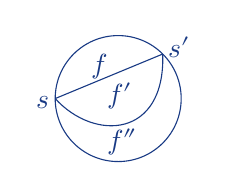
\begin{tikzpicture}[draw=blue,text=blue]\draw (0,0) circle (0.8); \draw (-0.8,0)--(0.5657,0.5657); \draw (-0.8,0) .. controls (-0.3,-0.55) and (0.6,-0.5) .. (0.5657,0.5657); \node at (-0.25,0.4) {$f$}; \node at (0.03,0.03) {$f'$}; \node at (0.05,-0.55) {$f''$}; \node at (-0.95,-0.05) {$s$}; \node at (0.78,0.65) {$s'$};\end{tikzpicture}} $f \cap f'' = \{s,s'\} = S_0$}
ness" condition is now expressed by demanding that the set of indices
I can be totally ordered, \var{\inserted[typed]{i.e. numbered}}{i.e. numbered}{typed insertion}{ps_134-2_027-v0011} in such a way that we get X by succesively
"attaching" \unsure{Dells|cells} $D_{n(i)}$ to the space already constructed\var{\xout{\unsure{,}}}{}{typewriter deletion}{ps_134-2_027-v0012} X(i-1), by a
map from \var{\deleted{a}}{}{deletion}{ps_134-2_027-v0013}\var{\inserted{a sub-}}{\hand{a sub-}}{insertion}{ps_134-2_027-v0014} cell \var{\xout{$D_i$}}{}{typewriter deletion}{ps_134-2_027-v0015}\var{\inserted{of $D_{n(i)}$}}{\hand{of $D_{n(i)}$}}{insertion}{ps_134-2_027-v0016}, $S_j^{\hand{\varepsilon}} \hand{\to} X(i-1)$ \quad $(\hand{\varepsilon\in\{}\pm 1\hand{\}})$ , this map of course
inducing an isomorphism,  more precisely \uline{the} standard isomorphism,\var{\inserted{$\varphi^{\unsure{\varepsilon'}}_{n(i')}$}}{\hand{$\varphi^{\unsure{\varepsilon'}}_{n(i')}$}}{insertion}{ps_134-2_027-v0017}\var{\deleted{of}}{}{deletion}{ps_134-2_027-v0018}
\margin{\textcircled{$\varphi^{\varepsilon'}_{n(i),j}$}}
$S_j^{\hand{\varepsilon}} \hand{\simeq} D_j$ \quad with\var{\inserted{$S^{\varepsilon'}_j$}}{\hand{$S^{\varepsilon'}_j$}}{insertion}{ps_134-2_027-v0019} one of the two corresponding cells $S_j^+$ , $S_j^-$ in some
\margin{\textcircled{$S^{\varepsilon'}_j$}}
$X_{i'} \hand{\simeq} D_{n(i')}$ .  The \var{\xout{xxxxx}}{}{typewriter deletion}{ps_134-2_027-v0020} dual translation of this\hand{,}in terms\hand{\unsure{$\vert$}} of fiber
products in \var{\xout{xxx}}{}{typewriter deletion}{ps_134-2_027-v0021} a category C endowed with objects $F_i$ $(i\in\underline{N})$ and maps
$s_1^i , t_1^i$ between these, is clear:  for a given set of indices I and map
\margin{$P=\prod_{i\in I}F_{n(i)}$}
$i \hand{\mapsto} n(i) : I \hand{\to} \underline{N}$ , we consider a sub\var{\xout{xxx}}{}{typewriter deletion}{ps_134-2_027-v0022}\var{\inserted[typed]{-object}}{-object}{typed insertion}{ps_134-2_027-v0023}\var{\inserted{ of}}{\hand{ of}}{insertion}{ps_134-2_027-v0024} $\var{\inserted[typed]{P=}}{P=}{typed insertion}{ps_134-2_027-v0025}\hand{\prod_{i\in I}}F_{n(i)}$ ,  which can be
described by equality relations between it\var{\over{t}{e}}{\hand{e}}{writing over}{ps_134-2_027-v0026}rated sources and targets
\var{\xout{xxxxxx}}{}{typewriter deletion}{ps_134-2_027-v0027} of various components of $u = (u_i)_{i\in I}$  in P,  the structure of
the set of relations being such that I can\hand{\unsure{,}}be numbered, from 1 to N say,
in such a way that we get in succession \var{\deleted{N}}{}{deletion}{ps_134-2_027-v0028}\var{\inserted{$N-1$}}{\hand{$N-1$}}{insertion}{ps_134-2_027-v0029} relations on the N components
$u_i$ respectively,\var{\inserted{$(2\leq i \leq N)$}}{\hand{$(2\leq i \leq N)$}}{insertion}{ps_134-2_027-v0030} every relation being of the type $f(u_i) = g(u_{i'})$ , with
f and g being iterated source or target maps, and $i'<i$ . \hand{(Whether}
\hand{source or target depending in obvious way on the two signs $\varepsilon,\varepsilon'$.)}

\mspage{\hand{27}}

%% END SOURCE ps_134-2_027
\ifnum\EditionMode=1
\psapparatusstart
\psentry{ps_134-2_027-v0001}{1}{deletion}{\deleted{\illegible{1}}}{}{The author cancels this material by hand; it leaves the corrected running text.}
\psentry{ps_134-2_027-v0002}{2}{insertion}{\inserted{(rather, finite $\varinjlim$'s)}}{\hand{(rather, finite $\varinjlim$'s)}}{The handwritten insertion is incorporated at its indicated position; insertion brackets leave the running text.}
\psentry{ps_134-2_027-v0003}{3}{typewriter deletion}{\xout{\unsure{s}}}{}{The typewriter strikes out this material; it leaves the corrected running text.}
\psentry{ps_134-2_027-v0004}{4}{deletion}{\deleted{cell}}{}{The author cancels this material by hand; it leaves the corrected running text.}
\psentry{ps_134-2_027-v0005}{5}{insertion}{\inserted{cells}}{\hand{cells}}{The handwritten insertion is incorporated at its indicated position; insertion brackets leave the running text.}
\psentry{ps_134-2_027-v0006}{6}{typewriter deletion}{\xout{\unsure{s}}}{}{The typewriter strikes out this material; it leaves the corrected running text.}
\psentry{ps_134-2_027-v0007}{7}{deletion}{\deleted{\illegible{3}}}{}{The author cancels this material by hand; it leaves the corrected running text.}
\psentry{ps_134-2_027-v0008}{8}{insertion}{\inserted{(12)}}{\hand{(12)}}{The handwritten insertion is incorporated at its indicated position; insertion brackets leave the running text.}
\psentry{ps_134-2_027-v0009}{9}{deletion}{\deleted{\illegible{2}}}{}{The author cancels this material by hand; it leaves the corrected running text.}
\psentry{ps_134-2_027-v0010}{10}{writing over}{\over{t}{d}}{\hand{d}}{The superposed handwritten reading replaces the underlying reading.}
\psentry{ps_134-2_027-v0011}{11}{typed insertion}{\inserted[typed]{i.e. numbered}}{i.e. numbered}{The typed insertion is incorporated at its indicated position; insertion brackets leave the running text.}
\psentry{ps_134-2_027-v0012}{12}{typewriter deletion}{\xout{\unsure{,}}}{}{The typewriter strikes out this material; it leaves the corrected running text.}
\psentry{ps_134-2_027-v0013}{13}{deletion}{\deleted{a}}{}{The author cancels this material by hand; it leaves the corrected running text.}
\psentry{ps_134-2_027-v0014}{14}{insertion}{\inserted{a sub-}}{\hand{a sub-}}{The handwritten insertion is incorporated at its indicated position; insertion brackets leave the running text.}
\psentry{ps_134-2_027-v0015}{15}{typewriter deletion}{\xout{$D_i$}}{}{The typewriter strikes out this material; it leaves the corrected running text.}
\psentry{ps_134-2_027-v0016}{16}{insertion}{\inserted{of $D_{n(i)}$}}{\hand{of $D_{n(i)}$}}{The handwritten insertion is incorporated at its indicated position; insertion brackets leave the running text.}
\psentry{ps_134-2_027-v0017}{17}{insertion}{\inserted{$\varphi^{\unsure{\varepsilon'}}_{n(i')}$}}{\hand{$\varphi^{\unsure{\varepsilon'}}_{n(i')}$}}{The handwritten insertion is incorporated at its indicated position; insertion brackets leave the running text.}
\psentry{ps_134-2_027-v0018}{18}{deletion}{\deleted{of}}{}{The author cancels this material by hand; it leaves the corrected running text.}
\psentry{ps_134-2_027-v0019}{19}{insertion}{\inserted{$S^{\varepsilon'}_j$}}{\hand{$S^{\varepsilon'}_j$}}{The handwritten insertion is incorporated at its indicated position; insertion brackets leave the running text.}
\psentry{ps_134-2_027-v0020}{20}{typewriter deletion}{\xout{xxxxx}}{}{The typewriter strikes out this material; it leaves the corrected running text.}
\psentry{ps_134-2_027-v0021}{21}{typewriter deletion}{\xout{xxx}}{}{The typewriter strikes out this material; it leaves the corrected running text.}
\psentry{ps_134-2_027-v0022}{22}{typewriter deletion}{\xout{xxx}}{}{The typewriter strikes out this material; it leaves the corrected running text.}
\psentry{ps_134-2_027-v0023}{23}{typed insertion}{\inserted[typed]{-object}}{-object}{The typed insertion is incorporated at its indicated position; insertion brackets leave the running text.}
\psentry{ps_134-2_027-v0024}{24}{insertion}{\inserted{ of}}{\hand{ of}}{The handwritten insertion is incorporated at its indicated position; insertion brackets leave the running text.}
\psentry{ps_134-2_027-v0025}{25}{typed insertion}{$\inserted[typed]{P=}$}{$P=$}{The typed insertion is incorporated at its indicated position; insertion brackets leave the running text.}
\psentry{ps_134-2_027-v0026}{26}{writing over}{\over{t}{e}}{\hand{e}}{The superposed handwritten reading replaces the underlying reading.}
\psentry{ps_134-2_027-v0027}{27}{typewriter deletion}{\xout{xxxxxx}}{}{The typewriter strikes out this material; it leaves the corrected running text.}
\psentry{ps_134-2_027-v0028}{28}{deletion}{\deleted{N}}{}{The author cancels this material by hand; it leaves the corrected running text.}
\psentry{ps_134-2_027-v0029}{29}{insertion}{\inserted{$N-1$}}{\hand{$N-1$}}{The handwritten insertion is incorporated at its indicated position; insertion brackets leave the running text.}
\psentry{ps_134-2_027-v0030}{30}{insertion}{\inserted{$(2\leq i \leq N)$}}{\hand{$(2\leq i \leq N)$}}{The handwritten insertion is incorporated at its indicated position; insertion brackets leave the running text.}
\psapparatusend
\fi
\pssource{ps_134-2_028}{134-2/28}{https://grothendieck.umontpellier.fr/web/viewer.html?file=../134-2.pdf\#page=29}
\psnumber{ps_134-2_028-v0001}{1}
\psnumber{ps_134-2_028-v0002}{2}
\psnumber{ps_134-2_028-v0003}{3}
\psnumber{ps_134-2_028-v0004}{4}
\psnumber{ps_134-2_028-v0005}{5}
\psnumber{ps_134-2_028-v0006}{6}
\psnumber{ps_134-2_028-v0007}{7}
\psnumber{ps_134-2_028-v0008}{8}
\psnumber{ps_134-2_028-v0009}{9}
\psnumber{ps_134-2_028-v0010}{10}
\psnumber{ps_134-2_028-v0011}{11}
\psnumber{ps_134-2_028-v0012}{12}
\psnumber{ps_134-2_028-v0013}{13}
\psnumber{ps_134-2_028-v0014}{14}
\psnumber{ps_134-2_028-v0015}{15}
\psnumber{ps_134-2_028-v0016}{16}
\psnumber{ps_134-2_028-v0017}{17}
\psnumber{ps_134-2_028-v0018}{18}
\psnumber{ps_134-2_028-v0019}{19}
\psnumber{ps_134-2_028-v0020}{20}
\psnumber{ps_134-2_028-v0021}{21}
\psnumber{ps_134-2_028-v0022}{22}
%% BEGIN SOURCE ps_134-2_028
% Pursuing Stacks (cotes 134-2 to 134-8): archive cote 134-2, site page 28 (PDF page 29).
% letter to Quillen. Draft compared: ps1.tex:660-736.
% AI-transcribed by Claude Opus 5.5 (claude-opus-5-5, adaptive thinking, effort high), Message Batches API, batch ps1 (msgbatch_01Rv5hCaNTtUt4JHx1yqoHPL), 2026-11-12; reviewed against both supplied scan halves; see CHECK_DECISIONS.tsv.
\scanpage{134-2/28}
\margin{8}
\mspage{\var{\deleted{\hand{8}}}{}{deletion}{ps_134-2_028-v0001} \hand{14}}
21.2.

\var{\over{\unsure{4}}{8}}{\hand{8}}{writing over}{ps_134-2_028-v0002}. Returning to theamalgamated sum $X = \hand{\bigcup_i}X_i$ , the cellular decompositions
of the components $X_i \hand{\simeq} D_{n(i)}$ define a cellular decomposition of X, whose
set of cells with incidence relation forms a finite ordered set K, fini-%
te union of a family of subsets $(K_i)_{i\in I}$ , with given isomorphisms\var{\xout{m}}{}{typewriter deletion}{ps_134-2_028-v0003}
\[ f_i : K_i \hand{\simeq} \underline{J}_{n(i)} \quad (i\in I) , \]
where for every index $n\in \underline{N}$, $\underline{J}_n$ denotes the ordered set of the 2n+1
cells $S_j^{\hand{\varepsilon}}$ $(0\leq j\leq n-1,\ \hand{\varepsilon\in\{}\pm 1\hand{\}})$, $D_n$ of the \var{\deleted{pertinent}}{}{deletion}{ps_134-2_028-v0004} \var{\inserted{relevant}}{\hand{relevant}}{insertion}{ps_134-2_028-v0005} cellular decomposition
of $D_n$ . We may without loss of generality assume there is no\var{\deleted{t}}{}{deletion}{ps_134-2_028-v0006} inclusion
relation between the $K_i$ , moreover the standar\var{\over{t}{d}}{\hand{d}}{writing over}{ps_134-2_028-v0007}ness condition described
above readily translates into a condition on this structure
$K$, $(K_i)_{i\in I}$ , $(f_i)_{i\in I}$ , and implies that for $i,i'\in I$, $K_i\hand{\cap}K_{i'}$ is a``clo-%
sed'' subset in the two ordered sets $K_i,K_{i'}$ (namely contains with any
element x the elements smaller than x), and moreover isomorphic (for the
induced order) to some $\underline{J}_n$ . Thus the category $B_o$ \var{\xout{is}}{}{typewriter deletion}{ps_134-2_028-v0008} can be viewed as the
category of such ``standar\var{\over{t}{d}}{\hand{d}}{writing over}{ps_134-2_028-v0009} ordered sets'' (with the extra structure on the-%
se just said), and the category $C_o$ can be defined most simply as the
dual category $B_o^{\,o}$ . (NB the definition of morphisms in $B_o$ is clear I
guess ...) I believe the category $B_o$ is stable under amalgamated sums
$X\hand{\amalg}_Z Y$ , provided \var{\inserted[typed]{however}}{however}{typed insertion}{ps_134-2_028-v0010} we insist that the empty structure K is \uline{not} allowed -
otherwise we have to \var{\xout{insist}}{}{typewriter deletion}{ps_134-2_028-v0011} restrict to amalgamated sums with $Z \neq \emptyset$ .
It seems finally more convenient to exclude the empty structure in $B_o$ ,
\margin{(13!)}
i.e. to exclude final element from $\underline{C}_o$ , for the benefit of being able to
\margin{\unsure{* This is obviously false, see P.S. p.12}}
state that $\underline{C}_o$ (and \uwave{all categories $\underline{C}_n$}\hand{*} \var{\deleted{\illegible{1}}}{}{deletion}{ps_134-2_028-v0012} \var{\xout{\illegible{1}}}{}{typewriter deletion}{ps_134-2_028-v0013} \var{\inserted{(13!))}}{\hand{(13!))}}{insertion}{ps_134-2_028-v0014} are stable under binary
amalgamated sums, and that the functors $\underline{C}_n\hand{\to} C$ (and ultimately $\underline{C}_\infty\hand{\to} C$)
we are interested in are just those commuting to arbitrary binary amalga-%
mated sums (without \var{\xout{\illegible{1}}}{}{typewriter deletion}{ps_134-2_028-v0015} awkward reference to the objects $\underline{F}_i$ and the
iterated source and target maps between them ...)\hand{(13!)}.

\var{\over{\illegible{1}}{9}}{\hand{9}}{writing over}{ps_134-2_028-v0016}. The category $\underline{C}_o$ being fairly well understood, \var{\inserted{it}}{\hand{it}}{insertion}{ps_134-2_028-v0017} remains to complete
the construction by the inductive step, \var{\inserted{for}}{\hand{for}}{insertion}{ps_134-2_028-v0018} passing from $\underline{C}_n$ to $\underline{C}_{n+1}$ . The
main properties I have in mind \var{\deleted{therefore}}{}{deletion}{ps_134-2_028-v0019} \var{\inserted{for this}}{\hand{for this}}{insertion}{ps_134-2_028-v0020}, for the sequence of categories
$\underline{C}_n$ and their limit $\underline{C}_\infty$ , are the following two.

A) For any $K\in Ob(\underline{C}_\infty)$ \ ($= Ob(\underline{C}_o)$), and any two arrows in $\underline{C}_\infty$
\[ f,g : K \hand{\rightrightarrows} F_i , \]
with $i\in\underline{N}$, \hand{(}and such that either i=0, or the equalities
\[ \hand{(1)}\qquad s_1^i f = s_1^i g \ , \quad t_1^i f = t_1^i g \]
hold (case $i \var{\over{>}{\geq}}{\hand{\geq}}{writing over}{ps_134-2_028-v0021} 1$), there exists $h: K\hand{\to} F_{i+1}$ such that
\[ \hand{(2)}\qquad s_1^{i+1} h = f \ , \quad t_1^{i+1} h = g \ . \]
B) For any $n\in\underline{N}$, the category $\underline{C}_{n+1}$ is deduced from $\underline{C}_n$ by keeping
the same objects, and just adding new arrows \var{\xout{\illegible{1}}}{}{typewriter deletion}{ps_134-2_028-v0022} h as in A), with
f, g arrows in $\underline{C}_n$ .

\margin{28}

%% END SOURCE ps_134-2_028
\ifnum\EditionMode=1
\psapparatusstart
\psentry{ps_134-2_028-v0001}{1}{deletion}{\deleted{\hand{8}}}{}{The author cancels this material by hand; it leaves the corrected running text.}
\psentry{ps_134-2_028-v0002}{2}{writing over}{\over{\unsure{4}}{8}}{\hand{8}}{The superposed handwritten reading replaces the underlying reading.}
\psentry{ps_134-2_028-v0003}{3}{typewriter deletion}{\xout{m}}{}{The typewriter strikes out this material; it leaves the corrected running text.}
\psentry{ps_134-2_028-v0004}{4}{deletion}{\deleted{pertinent}}{}{The author cancels this material by hand; it leaves the corrected running text.}
\psentry{ps_134-2_028-v0005}{5}{insertion}{\inserted{relevant}}{\hand{relevant}}{The handwritten insertion is incorporated at its indicated position; insertion brackets leave the running text.}
\psentry{ps_134-2_028-v0006}{6}{deletion}{\deleted{t}}{}{The author cancels this material by hand; it leaves the corrected running text.}
\psentry{ps_134-2_028-v0007}{7}{writing over}{\over{t}{d}}{\hand{d}}{The superposed handwritten reading replaces the underlying reading.}
\psentry{ps_134-2_028-v0008}{8}{typewriter deletion}{\xout{is}}{}{The typewriter strikes out this material; it leaves the corrected running text.}
\psentry{ps_134-2_028-v0009}{9}{writing over}{\over{t}{d}}{\hand{d}}{The superposed handwritten reading replaces the underlying reading.}
\psentry{ps_134-2_028-v0010}{10}{typed insertion}{\inserted[typed]{however}}{however}{The typed insertion is incorporated at its indicated position; insertion brackets leave the running text.}
\psentry{ps_134-2_028-v0011}{11}{typewriter deletion}{\xout{insist}}{}{The typewriter strikes out this material; it leaves the corrected running text.}
\psentry{ps_134-2_028-v0012}{12}{deletion}{\deleted{\illegible{1}}}{}{The author cancels this material by hand; it leaves the corrected running text.}
\psentry{ps_134-2_028-v0013}{13}{typewriter deletion}{\xout{\illegible{1}}}{}{The typewriter strikes out this material; it leaves the corrected running text.}
\psentry{ps_134-2_028-v0014}{14}{insertion}{\inserted{(13!))}}{\hand{(13!))}}{The handwritten insertion is incorporated at its indicated position; insertion brackets leave the running text.}
\psentry{ps_134-2_028-v0015}{15}{typewriter deletion}{\xout{\illegible{1}}}{}{The typewriter strikes out this material; it leaves the corrected running text.}
\psentry{ps_134-2_028-v0016}{16}{writing over}{\over{\illegible{1}}{9}}{\hand{9}}{The superposed handwritten reading replaces the underlying reading.}
\psentry{ps_134-2_028-v0017}{17}{insertion}{\inserted{it}}{\hand{it}}{The handwritten insertion is incorporated at its indicated position; insertion brackets leave the running text.}
\psentry{ps_134-2_028-v0018}{18}{insertion}{\inserted{for}}{\hand{for}}{The handwritten insertion is incorporated at its indicated position; insertion brackets leave the running text.}
\psentry{ps_134-2_028-v0019}{19}{deletion}{\deleted{therefore}}{}{The author cancels this material by hand; it leaves the corrected running text.}
\psentry{ps_134-2_028-v0020}{20}{insertion}{\inserted{for this}}{\hand{for this}}{The handwritten insertion is incorporated at its indicated position; insertion brackets leave the running text.}
\psentry{ps_134-2_028-v0021}{21}{writing over}{$\over{>}{\geq}$}{$\hand{\geq}$}{The superposed handwritten reading replaces the underlying reading.}
\psentry{ps_134-2_028-v0022}{22}{typewriter deletion}{\xout{\illegible{1}}}{}{The typewriter strikes out this material; it leaves the corrected running text.}
\psapparatusend
\fi
\pssource{ps_134-2_029}{134-2/29}{https://grothendieck.umontpellier.fr/web/viewer.html?file=../134-2.pdf\#page=30}
\psnumber{ps_134-2_029-v0001}{1}
\psnumber{ps_134-2_029-v0002}{2}
\psnumber{ps_134-2_029-v0003}{3}
\psnumber{ps_134-2_029-v0004}{4}
\psnumber{ps_134-2_029-v0005}{5}
\psnumber{ps_134-2_029-v0006}{6}
\psnumber{ps_134-2_029-v0007}{7}
\psnumber{ps_134-2_029-v0008}{8}
\psnumber{ps_134-2_029-v0009}{9}
\psnumber{ps_134-2_029-v0010}{10}
\psnumber{ps_134-2_029-v0011}{11}
\psnumber{ps_134-2_029-v0012}{12}
\psnumber{ps_134-2_029-v0013}{13}
\psnumber{ps_134-2_029-v0014}{14}
\psnumber{ps_134-2_029-v0015}{15}
\psnumber{ps_134-2_029-v0016}{16}
\psnumber{ps_134-2_029-v0017}{17}
\psnumber{ps_134-2_029-v0018}{18}
\psnumber{ps_134-2_029-v0019}{19}
\psnumber{ps_134-2_029-v0020}{20}
\psnumber{ps_134-2_029-v0021}{21}
\psnumber{ps_134-2_029-v0022}{22}
\psnumber{ps_134-2_029-v0023}{23}
\psnumber{ps_134-2_029-v0024}{24}
\psnumber{ps_134-2_029-v0025}{25}
\psnumber{ps_134-2_029-v0026}{26}
\psnumber{ps_134-2_029-v0027}{27}
\psnumber{ps_134-2_029-v0028}{28}
\psnumber{ps_134-2_029-v0029}{29}
\psnumber{ps_134-2_029-v0030}{30}
\psnumber{ps_134-2_029-v0031}{31}
\psnumber{ps_134-2_029-v0032}{32}
\psnumber{ps_134-2_029-v0033}{33}
\psnumber{ps_134-2_029-v0034}{34}
\psnumber{ps_134-2_029-v0035}{35}
\psnumber{ps_134-2_029-v0036}{36}
\psnumber{ps_134-2_029-v0037}{37}
\psnumber{ps_134-2_029-v0038}{38}
\psnumber{ps_134-2_029-v0039}{39}
%% BEGIN SOURCE ps_134-2_029
% Pursuing Stacks (cotes 134-2 to 134-8): archive cote 134-2, site page 29 (PDF page 30).
% letter to Quillen. Draft compared: ps1.tex:723-786.
% AI-transcribed by Claude Opus 5.5 (claude-opus-5-5, adaptive thinking, effort high), Message Batches API, batch ps1 (msgbatch_01Rv5hCaNTtUt4JHx1yqoHPL), 2026-11-12; reviewed against both supplied scan halves; see CHECK_DECISIONS.tsv.
\scanpage{134-2/29}
\mspage{\hand{\unsure{1|\#}5}}

The expression ``deduce\var{\over{s}{d}}{\hand{d}}{writing over}{ps_134-2_029-v0001} from'' in B)  means that we are adding arrows
$h: K \hand{\to} F_i$ (each with preassigned source and target in $\underline{C}_n$),  with as
``new axioms'' on \var{\inserted[typed]{the bunch of}}{the bunch of}{typed insertion}{ps_134-2_029-v0002} these uniquely the two relations \var{\deleted{\illegible{1}}}{}{deletion}{ps_134-2_029-v0003}\var{\inserted{(1),(2)}}{\hand{(1),(2)}}{insertion}{ps_134-2_029-v0004} of \var{\over{\illegible{1}}{A}}{\hand{A}}{writing over}{ps_134-2_029-v0005}), the category
$\underline{C}_{n+1}$  being deduced from $\underline{C}_n$ in an obvious way,  as the solution of a uni-%
versal problem with\var{\inserted{in}}{\hand{in}}{insertion}{ps_134-2_029-v0006} the category of all categories where binary amalgama-%
ted products exist,  and ``maps'' between these being functors which commute
\margin{\unsure{this has to be corrected -- amalgamated sums exist in $\underline{C}_o$ only, and \uline{\unsure{those|these}} \unsure{sh\textsuperscript{d}|sh\textsuperscript{ld}} be respected}}
to those fibered products\var{\inserted{(14!)}}{\hand{(14!)}}{insertion}{ps_134-2_029-v0007}. \var{\deleted{In}}{}{deletion}{ps_134-2_029-v0008}\var{\inserted{In}}{\hand{In}}{insertion}{ps_134-2_029-v0009} practical terms,  the arrows of $\underline{C}_{n+1}$ are
those deduced from the arrows in $\underline{C}_n$ and the ``new'' arrows $h$,  by combining
formal operations of composing arrows by $v\circ u$ ,  and taking \var{\inserted{(binary)}}{\hand{(binary)}}{insertion}{ps_134-2_029-v0010} amalgamated
products of arrows. \var{\deleted{\illegible{1}}}{}{deletion}{ps_134-2_029-v0011}

NB  Of course the condition (1) in A) is necessary for the existence
\margin{$\|$}of an $h$ satisfying (2).  That it is sufficient too \var{\deleted{can}}{}{deletion}{ps_134-2_029-v0012}\var{\inserted{may}}{\hand{may}}{insertion}{ps_134-2_029-v0013} be viewed as an
extremely strong,\var{\xout{\unsure{version}}}{}{typewriter deletion}{ps_134-2_029-v0014} ``universal'' version of coherence conditions,
concerning the various structures introduced on a $\infty$-groupoid. Intuitive-%
ly,  it means that whenever we have \var{\deleted{\over{\illegible{1}}{two} ways of}}{}{deletion}{ps_134-2_029-v0015}\var{\inserted{two ways of}}{\hand{two ways of}}{insertion}{ps_134-2_029-v0016} associating to a \var{\inserted[typed]{finite}}{finite}{typed insertion}{ps_134-2_029-v0017} family \var{\deleted{\illegible{1}}}{}{deletion}{ps_134-2_029-v0018}
$(u_i)_{i\in I}$  of objects of an $\infty$-groupoid,  $u_i \in F_{n(i)}$ ,  \var{\xout{xxxxxxxxxx}}{}{typewriter deletion}{ps_134-2_029-v0019} subjected
to a \hand{``}standar\var{\over{t}{d}}{\hand{d}}{writing over}{ps_134-2_029-v0020}\hand{''} set of relations on the $u_i$'s, an element of some $F_n$ ,  in
terms of the $\infty$-groupoid structure only,  then we have automatically
\var{\inserted[typed]{a ``homotopy''}}{a ``homotopy''}{typed insertion}{ps_134-2_029-v0021}\var{\xout{an isomorphism}}{}{typewriter deletion}{ps_134-2_029-v0022} between these built-in in the very structure of the $\infty$-%
groupoid,  provided it makes at all a sense to ask for one (namely provi-%
ded condition (1) holds if $n \geq 1$).   I have the feeling moreover that
conditions (A) and (B) (plus the relation $\underline{C}_\infty = \mathop{\mathrm{lim}}\limits_{\hand{\longrightarrow}} \underline{C}_n$ ) is all what will
be ever needed,  when using the definition of the structure species,
- plus of course the description of $\underline{C}_o$ , and the \var{\inserted[typed]{implicit}}{implicit}{typed insertion}{ps_134-2_029-v0023} fact that the categories
\margin{inaccurate -- see above}
$\underline{C}_n$ are stable under binary fiber products and the inclusion functors com-%
mute to these\var{\inserted{(13!)}}{\hand{(13!)}}{insertion}{ps_134-2_029-v0024}. Of course,  the category which really interests us is
$\underline{C}_\infty$,  the description of the intermediate $\underline{C}_n$'s\hand{$|$} is merely tec\var{\over{\illegible{1}}{h}}{\hand{h}}{writing over}{ps_134-2_029-v0025}nical \var{\deleted{txt}}{}{deletion}{ps_134-2_029-v0026} -
the main point is that there should exist an increasing sequence $(C_n)$ of
subcategories of $\underline{C}_\infty$ ,  having same objects\var{\over{,}{(}}{\hand{(}}{writing over}{ps_134-2_029-v0027}and ``same'' fiberproducts\var{\over{,}{)}}{\hand{)}}{writing over}{ps_134-2_029-v0028}\var{\inserted{(13!)}}{\hand{(13!)}}{insertion}{ps_134-2_029-v0029},
such that $\underline{C}_\infty$ should be the limit (i.e. every arrow in $C_\infty$ should belong \var{\deleted{\illegible{1}}}{}{deletion}{ps_134-2_029-v0030}
to some $\underline{C}_n$),  and such that the passage from $\underline{C}_n$ to $\underline{C}_{n+1}$ should satisfy \var{\inserted{(B).}}{\hand{(B).}}{insertion}{ps_134-2_029-v0031}
\var{\deleted{(B).}}{}{deletion}{ps_134-2_029-v0032} \var{\margin{\diagram{\begin{tikzpicture}\draw (0,0)--(.32,0)--(.32,.27)--(.68,.27);\end{tikzpicture}}}It is fairly obvious}{

It is fairly obvious}{author paragraph break}{ps_134-2_029-v0033} that these conditions alone do by no means
caracterise $\underline{C}_\infty$  up to equivalence,  and still less the sequence of its
subcategories $\underline{C}_n$ .  The point I wish to make though,  before pursuing
with a proposal of an explicit description,  is \var{\inserted{(firstly)}}{\hand{(firstly)}}{insertion}{ps_134-2_029-v0034} that \uline{this ambiguity is}
\uline{in the nature of things}\var{\over{,}{.}}{\hand{.}}{writing over}{ps_134-2_029-v0035} \var{\over{r}{R}}{\hand{R}}{writing over}{ps_134-2_029-v0036}oughly saying, two different mathematicians,
working independently on the conceptual problem I had in mind,  \var{\deleted{assuming}}{}{deletion}{ps_134-2_029-v0037}\var{\inserted{assuming}}{\hand{assuming}}{insertion}{ps_134-2_029-v0038}
they both wind up with some explicit definition,  will almost certainly
get non e\var{\over[typed]{\illegible{1}}{q}}{q}{typewriter overwriting}{ps_134-2_029-v0039}uivalent definitions  -  namely with non equivalent categories
of (set-valued, say) $\infty$-groupoids !  And, secondly and as importantly,

\mspage{29}

%% END SOURCE ps_134-2_029
\ifnum\EditionMode=1
\psapparatusstart
\psentry{ps_134-2_029-v0001}{1}{writing over}{\over{s}{d}}{\hand{d}}{The superposed handwritten reading replaces the underlying reading.}
\psentry{ps_134-2_029-v0002}{2}{typed insertion}{\inserted[typed]{the bunch of}}{the bunch of}{The typed insertion is incorporated at its indicated position; insertion brackets leave the running text.}
\psentry{ps_134-2_029-v0003}{3}{deletion}{\deleted{\illegible{1}}}{}{The author cancels this material by hand; it leaves the corrected running text.}
\psentry{ps_134-2_029-v0004}{4}{insertion}{\inserted{(1),(2)}}{\hand{(1),(2)}}{The handwritten insertion is incorporated at its indicated position; insertion brackets leave the running text.}
\psentry{ps_134-2_029-v0005}{5}{writing over}{\over{\illegible{1}}{A}}{\hand{A}}{The superposed handwritten reading replaces the underlying reading.}
\psentry{ps_134-2_029-v0006}{6}{insertion}{\inserted{in}}{\hand{in}}{The handwritten insertion is incorporated at its indicated position; insertion brackets leave the running text.}
\psentry{ps_134-2_029-v0007}{7}{insertion}{\inserted{(14!)}}{\hand{(14!)}}{The handwritten insertion is incorporated at its indicated position; insertion brackets leave the running text.}
\psentry{ps_134-2_029-v0008}{8}{deletion}{\deleted{In}}{}{The author cancels this material by hand; it leaves the corrected running text.}
\psentry{ps_134-2_029-v0009}{9}{insertion}{\inserted{In}}{\hand{In}}{The handwritten insertion is incorporated at its indicated position; insertion brackets leave the running text.}
\psentry{ps_134-2_029-v0010}{10}{insertion}{\inserted{(binary)}}{\hand{(binary)}}{The handwritten insertion is incorporated at its indicated position; insertion brackets leave the running text.}
\psentry{ps_134-2_029-v0011}{11}{deletion}{\deleted{\illegible{1}}}{}{The author cancels this material by hand; it leaves the corrected running text.}
\psentry{ps_134-2_029-v0012}{12}{deletion}{\deleted{can}}{}{The author cancels this material by hand; it leaves the corrected running text.}
\psentry{ps_134-2_029-v0013}{13}{insertion}{\inserted{may}}{\hand{may}}{The handwritten insertion is incorporated at its indicated position; insertion brackets leave the running text.}
\psentry{ps_134-2_029-v0014}{14}{typewriter deletion}{\xout{\unsure{version}}}{}{The typewriter strikes out this material; it leaves the corrected running text.}
\psentry{ps_134-2_029-v0015}{15}{deletion}{\deleted{\over{\illegible{1}}{two} ways of}}{}{The author cancels this material by hand; it leaves the corrected running text.}
\psentry{ps_134-2_029-v0016}{16}{insertion}{\inserted{two ways of}}{\hand{two ways of}}{The handwritten insertion is incorporated at its indicated position; insertion brackets leave the running text.}
\psentry{ps_134-2_029-v0017}{17}{typed insertion}{\inserted[typed]{finite}}{finite}{The typed insertion is incorporated at its indicated position; insertion brackets leave the running text.}
\psentry{ps_134-2_029-v0018}{18}{deletion}{\deleted{\illegible{1}}}{}{The author cancels this material by hand; it leaves the corrected running text.}
\psentry{ps_134-2_029-v0019}{19}{typewriter deletion}{\xout{xxxxxxxxxx}}{}{The typewriter strikes out this material; it leaves the corrected running text.}
\psentry{ps_134-2_029-v0020}{20}{writing over}{\over{t}{d}}{\hand{d}}{The superposed handwritten reading replaces the underlying reading.}
\psentry{ps_134-2_029-v0021}{21}{typed insertion}{\inserted[typed]{a ``homotopy''}}{a ``homotopy''}{The typed insertion is incorporated at its indicated position; insertion brackets leave the running text.}
\psentry{ps_134-2_029-v0022}{22}{typewriter deletion}{\xout{an isomorphism}}{}{The typewriter strikes out this material; it leaves the corrected running text.}
\psentry{ps_134-2_029-v0023}{23}{typed insertion}{\inserted[typed]{implicit}}{implicit}{The typed insertion is incorporated at its indicated position; insertion brackets leave the running text.}
\psentry{ps_134-2_029-v0024}{24}{insertion}{\inserted{(13!)}}{\hand{(13!)}}{The handwritten insertion is incorporated at its indicated position; insertion brackets leave the running text.}
\psentry{ps_134-2_029-v0025}{25}{writing over}{\over{\illegible{1}}{h}}{\hand{h}}{The superposed handwritten reading replaces the underlying reading.}
\psentry{ps_134-2_029-v0026}{26}{deletion}{\deleted{txt}}{}{The author cancels this material by hand; it leaves the corrected running text.}
\psentry{ps_134-2_029-v0027}{27}{writing over}{\over{,}{(}}{\hand{(}}{The superposed handwritten reading replaces the underlying reading.}
\psentry{ps_134-2_029-v0028}{28}{writing over}{\over{,}{)}}{\hand{)}}{The superposed handwritten reading replaces the underlying reading.}
\psentry{ps_134-2_029-v0029}{29}{insertion}{\inserted{(13!)}}{\hand{(13!)}}{The handwritten insertion is incorporated at its indicated position; insertion brackets leave the running text.}
\psentry{ps_134-2_029-v0030}{30}{deletion}{\deleted{\illegible{1}}}{}{The author cancels this material by hand; it leaves the corrected running text.}
\psentry{ps_134-2_029-v0031}{31}{insertion}{\inserted{(B).}}{\hand{(B).}}{The handwritten insertion is incorporated at its indicated position; insertion brackets leave the running text.}
\psentry{ps_134-2_029-v0032}{32}{deletion}{\deleted{(B).}}{}{The author cancels this material by hand; it leaves the corrected running text.}
\psentry{ps_134-2_029-v0033}{33}{author paragraph break}{\margin{\diagram{\begin{tikzpicture}\draw (0,0)--(.32,0)--(.32,.27)--(.68,.27);\end{tikzpicture}}}It is fairly obvious}{

It is fairly obvious}{The stepped pen cue at this boundary instructs a new paragraph; the diplomatic text retains its graphic.}
\psentry{ps_134-2_029-v0034}{34}{insertion}{\inserted{(firstly)}}{\hand{(firstly)}}{The handwritten insertion is incorporated at its indicated position; insertion brackets leave the running text.}
\psentry{ps_134-2_029-v0035}{35}{writing over}{\over{,}{.}}{\hand{.}}{The superposed handwritten reading replaces the underlying reading.}
\psentry{ps_134-2_029-v0036}{36}{writing over}{\over{r}{R}}{\hand{R}}{The superposed handwritten reading replaces the underlying reading.}
\psentry{ps_134-2_029-v0037}{37}{deletion}{\deleted{assuming}}{}{The author cancels this material by hand; it leaves the corrected running text.}
\psentry{ps_134-2_029-v0038}{38}{insertion}{\inserted{assuming}}{\hand{assuming}}{The handwritten insertion is incorporated at its indicated position; insertion brackets leave the running text.}
\psentry{ps_134-2_029-v0039}{39}{typewriter overwriting}{\over[typed]{\illegible{1}}{q}}{q}{The superposed typed reading replaces the underlying reading.}
\psapparatusend
\fi
\pssource{ps_134-2_030}{134-2/30}{https://grothendieck.umontpellier.fr/web/viewer.html?file=../134-2.pdf\#page=31}
\psnumber{ps_134-2_030-v0001}{1}
\psnumber{ps_134-2_030-v0002}{2}
\psnumber{ps_134-2_030-v0003}{3}
\psnumber{ps_134-2_030-v0004}{4}
\psnumber{ps_134-2_030-v0005}{5}
\psnumber{ps_134-2_030-v0006}{6}
\psnumber{ps_134-2_030-v0007}{7}
\psnumber{ps_134-2_030-v0008}{8}
\psnumber{ps_134-2_030-v0009}{9}
\psnumber{ps_134-2_030-v0010}{10}
\psnumber{ps_134-2_030-v0011}{11}
\psnumber{ps_134-2_030-v0012}{12}
\psnumber{ps_134-2_030-v0013}{13}
\psnumber{ps_134-2_030-v0014}{14}
\psnumber{ps_134-2_030-v0015}{15}
\psnumber{ps_134-2_030-v0016}{16}
\psnumber{ps_134-2_030-v0017}{17}
\psnumber{ps_134-2_030-v0018}{18}
\psnumber{ps_134-2_030-v0019}{19}
\psnumber{ps_134-2_030-v0020}{20}
\psnumber{ps_134-2_030-v0021}{21}
%% BEGIN SOURCE ps_134-2_030
% Pursuing Stacks (cotes 134-2 to 134-8): archive cote 134-2, site page 30 (PDF page 31).
% letter to Quillen. Draft compared: ps1.tex:771-835.
% AI-transcribed by Claude Opus 5.5 (claude-opus-5-5, adaptive thinking, effort high), Message Batches API, batch ps1 (msgbatch_01Rv5hCaNTtUt4JHx1yqoHPL), 2026-11-12; reviewed against both supplied scan halves; see CHECK_DECISIONS.tsv.
\scanpage{134-2/30}
\margin{9}
\mspage{\var{\deleted{\hand{9}}}{}{deletion}{ps_134-2_030-v0001} \hand{16}}
that \uline{this ambiguity however is an irrelevant one.} To make this point
a little clearer, I could say that a third mathematician, informed of
the work of both, will readily think out a functor or rather a pair of
functors, associati\var{\xout{m}}{}{typewriter deletion}{ps_134-2_030-v0002}ng to any \var{\over[typed]{\illegible{1}}{s}}{s}{typewriter overwriting}{ps_134-2_030-v0003}tructure of Mr. X one of Mr. Y and conver%
\hand{-}sely, in such a way that by composition of the two, we will associate
to a X-s\var{\over[typed]{\illegible{1}}{t}}{t}{typewriter overwriting}{ps_134-2_030-v0004}ructure \hand{(}T say\hand{)} another T', which \var{\deleted{of course}}{}{deletion}{ps_134-2_030-v0005} will not be isomor-%
phic to T of course, but endowed with a canonical \var{\xout{xxxx}}{}{typewriter deletion}{ps_134-2_030-v0006} $\infty$-equivalence
(in the sense of Mr. X) $T \hand{\underset{\infty}{\simeq}} T'$ , and the same on the Mr. Y side. Most
probably, a fourth mathematician, faced with the same situation as the
third, will get \var{\inserted[typed]{his own}}{his own}{typed insertion}{ps_134-2_030-v0007} \var{\xout{a different}}{}{typewriter deletion}{ps_134-2_030-v0008} pair of functors to reconciliate Mr X and Mr
Y , \var{\inserted[typed]{which}}{which}{typed insertion}{ps_134-2_030-v0009} \var{\xout{but}}{}{typewriter deletion}{ps_134-2_030-v0010} very probably \var{\xout{his pair of functors}}{}{typewriter deletion}{ps_134-2_030-v0011} won\hand{'}t be equivalent \var{\xout{\illegible{1}}}{}{typewriter deletion}{ps_134-2_030-v0012} \hand{(}I mean
isomorphic\hand{)} to the previous one. Here however a fifth mathematician,
informed about this new perplexity, will probably show that the two
Y-structures U and U', associated by his two colleagues to \var{\xout{the}}{}{typewriter deletion}{ps_134-2_030-v0013} an
X-structure T, while not isomorphic alas, admit however a canonical
$\infty$-equivalence between U and U'\var{\inserted[typed]{(in the sense of the Y-theory)}}{(in the sense of the Y-theory)}{typed insertion}{ps_134-2_030-v0014}. I could go on with a sixth mathematicia%
an, confronted with the same perplexity as the previous one, who winds
up with another \var{\inserted{$\infty$-}}{\hand{$\infty$-}}{insertion}{ps_134-2_030-v0015}equivalence between U and U' (without being informed of
the work of the fifth), and a seventh reconciling them by discovering
an $\infty$-equivalence between these equivalences. The story of course is
infinite, I better stop with seven mathematicians, a fair number now-%
adays to allow themselves getting involved with foundational matters ...
There should be a mathematical statement though resuming in finite terms
this infinite story, but in order to write it down I guess a minimum
amount of conceptual work, in the context of a given notion of $\infty$-grou-%
poids satisfying the desiderata (A) and (B) should be done, and I am by
no means sure I will go through this, not in this letter anyhow.

\var{\margin{\deleted{10.}}}{}{marginal note revised}{ps_134-2_030-v0016} \hand{10.} Now in the long last the explicit description I promised of $\underline{C}_{n+1}$ \var{\deleted{in}}{}{deletion}{ps_134-2_030-v0017} \var{\inserted{in}}{\hand{in}}{insertion}{ps_134-2_030-v0018}
terms of $\underline{C}_n$ . As a matter of fact, I have a handful to propose ! One \margin{\unsure{n}}
choice, about the widest I would think of, is: for every pair (f,g)
in $\underline{C}_n$ satisfying condition (1) of (A), add one \var{\xout{xxxxx}}{}{typewriter deletion}{ps_134-2_030-v0019} new arrow h. To
avoid set-theoretic difficulties though, we better \var{\xout{xxxxxx}}{}{typewriter deletion}{ps_134-2_030-v0020} first modify
the definition of $\underline{C}_o$ so that the set of its objects should be in the
universe we are working in, preferably even it be countable. Or else
and more reasonably, we will pick one h for every isomorphism class of
situations (f,g) in $\underline{C}_n$ . Another restriction\hand{,} to avoid too much redundan-%
cy - this was the first definition actually that flipped to my mind the
day before yesterday - is to add a \uline{new} h only when there is no ``old''
one, namely in $\underline{C}_n$ , serving the same purpose. Then it came to my mind
that there is a lot of redundancy still\hand{:} \var{\inserted[typed]{thus there would be already \deleted{in}}}{thus there would be already }{typed insertion}{ps_134-2_030-v0021}
\margin{30}

%% END SOURCE ps_134-2_030
\ifnum\EditionMode=1
\psapparatusstart
\psentry{ps_134-2_030-v0001}{1}{deletion}{\deleted{\hand{9}}}{}{The author cancels this material by hand; it leaves the corrected running text.}
\psentry{ps_134-2_030-v0002}{2}{typewriter deletion}{\xout{m}}{}{The typewriter strikes out this material; it leaves the corrected running text.}
\psentry{ps_134-2_030-v0003}{3}{typewriter overwriting}{\over[typed]{\illegible{1}}{s}}{s}{The superposed typed reading replaces the underlying reading.}
\psentry{ps_134-2_030-v0004}{4}{typewriter overwriting}{\over[typed]{\illegible{1}}{t}}{t}{The superposed typed reading replaces the underlying reading.}
\psentry{ps_134-2_030-v0005}{5}{deletion}{\deleted{of course}}{}{The author cancels this material by hand; it leaves the corrected running text.}
\psentry{ps_134-2_030-v0006}{6}{typewriter deletion}{\xout{xxxx}}{}{The typewriter strikes out this material; it leaves the corrected running text.}
\psentry{ps_134-2_030-v0007}{7}{typed insertion}{\inserted[typed]{his own}}{his own}{The typed insertion is incorporated at its indicated position; insertion brackets leave the running text.}
\psentry{ps_134-2_030-v0008}{8}{typewriter deletion}{\xout{a different}}{}{The typewriter strikes out this material; it leaves the corrected running text.}
\psentry{ps_134-2_030-v0009}{9}{typed insertion}{\inserted[typed]{which}}{which}{The typed insertion is incorporated at its indicated position; insertion brackets leave the running text.}
\psentry{ps_134-2_030-v0010}{10}{typewriter deletion}{\xout{but}}{}{The typewriter strikes out this material; it leaves the corrected running text.}
\psentry{ps_134-2_030-v0011}{11}{typewriter deletion}{\xout{his pair of functors}}{}{The typewriter strikes out this material; it leaves the corrected running text.}
\psentry{ps_134-2_030-v0012}{12}{typewriter deletion}{\xout{\illegible{1}}}{}{The typewriter strikes out this material; it leaves the corrected running text.}
\psentry{ps_134-2_030-v0013}{13}{typewriter deletion}{\xout{the}}{}{The typewriter strikes out this material; it leaves the corrected running text.}
\psentry{ps_134-2_030-v0014}{14}{typed insertion}{\inserted[typed]{(in the sense of the Y-theory)}}{(in the sense of the Y-theory)}{The typed insertion is incorporated at its indicated position; insertion brackets leave the running text.}
\psentry{ps_134-2_030-v0015}{15}{insertion}{\inserted{$\infty$-}}{\hand{$\infty$-}}{The handwritten insertion is incorporated at its indicated position; insertion brackets leave the running text.}
\psentry{ps_134-2_030-v0016}{16}{marginal note revised}{\margin{\deleted{10.}}}{}{The author's internal cancellations and replacements in this marginal note are applied at its source-line call.}
\psentry{ps_134-2_030-v0017}{17}{deletion}{\deleted{in}}{}{The author cancels this material by hand; it leaves the corrected running text.}
\psentry{ps_134-2_030-v0018}{18}{insertion}{\inserted{in}}{\hand{in}}{The handwritten insertion is incorporated at its indicated position; insertion brackets leave the running text.}
\psentry{ps_134-2_030-v0019}{19}{typewriter deletion}{\xout{xxxxx}}{}{The typewriter strikes out this material; it leaves the corrected running text.}
\psentry{ps_134-2_030-v0020}{20}{typewriter deletion}{\xout{xxxxxx}}{}{The typewriter strikes out this material; it leaves the corrected running text.}
\psentry{ps_134-2_030-v0021}{21}{typed insertion}{\inserted[typed]{thus there would be already \deleted{in}}}{thus there would be already }{The typed insertion is incorporated at its indicated position; insertion brackets leave the running text.}
\psapparatusend
\fi
\pssource{ps_134-2_031}{134-2/31}{https://grothendieck.umontpellier.fr/web/viewer.html?file=../134-2.pdf\#page=32}
\psnumber{ps_134-2_031-v0001}{1}
\psnumber{ps_134-2_031-v0002}{2}
\psnumber{ps_134-2_031-v0003}{3}
\psnumber{ps_134-2_031-v0004}{4}
\psnumber{ps_134-2_031-v0005}{5}
\psnumber{ps_134-2_031-v0006}{6}
\psnumber{ps_134-2_031-v0007}{7}
\psnumber{ps_134-2_031-v0008}{8}
\psnumber{ps_134-2_031-v0009}{9}
\psnumber{ps_134-2_031-v0010}{10}
\psnumber{ps_134-2_031-v0011}{11}
\psnumber{ps_134-2_031-v0012}{12}
\psnumber{ps_134-2_031-v0013}{13}
\psnumber{ps_134-2_031-v0014}{14}
\psnumber{ps_134-2_031-v0015}{15}
\psnumber{ps_134-2_031-v0016}{16}
\psnumber{ps_134-2_031-v0017}{17}
%% BEGIN SOURCE ps_134-2_031
% Pursuing Stacks (cotes 134-2 to 134-8): archive cote 134-2, site page 31 (PDF page 32).
% letter to Quillen. Draft compared: ps1.tex:823-894.
% AI-transcribed by Claude Opus 5.5 (claude-opus-5-5, adaptive thinking, effort high), Message Batches API, batch ps1 (msgbatch_01Rv5hCaNTtUt4JHx1yqoHPL), 2026-11-12; reviewed against both supplied scan halves; see CHECK_DECISIONS.tsv.
\scanpage{134-2/31}
\mspage{\hand{17}}
infinitely many ope\var{\xout{x}}{}{typewriter deletion}{ps_134-2_031-v0001}rations standing for the single ope\var{\over[typed]{\illegible{1}}{rat}}{rat}{typewriter overwriting}{ps_134-2_031-v0002}ion $v\overset{i}{\circ}u$ say,
which could be \var{wiewed}{viewed}{slip corrected}{ps_134-2_031-v0003} in effect in terms of an arbitrary n-sequence
($n\geqslant 2$) of "composable" i-objects $U_1=u,u_2=v,\ u_3.\dots\ u_n$ ;\var{\inserted{just ``forgetting'' $u_3,\dots,u_n$!}}{\hand{just ``forgetting'' $u_3,\dots,u_n$!}}{insertion}{ps_134-2_031-v0004} The natural
way to meet this "objection" would be to restrict to \var{\xout{a}}{}{typewriter deletion}{ps_134-2_031-v0005} pairs (f,g)
which cannot be factored non trivially through another object $K'$ as
\diagram{\begin{tikzcd} K \ar[r, blue] \& K' \ar[r, shift left, blue, "{f',g'}"] \ar[r, shift right, blue] \& F_i \end{tikzcd} .}
But even with such restrictions, there remain a lot of redundancies
- and this again seems to me in the nature of things, namely that there
is no really natural, "most economic" way for achieving condition (A),
by a stepwise construction meeting condition (B). For instance, in $\underline{C}_1$
already we will have \var{\xout{the}}{}{typewriter deletion}{ps_134-2_031-v0006} not merely the compositions $v\overset{i}{\circ}u$ , but at the
same time simultaneous compositions
\[ (*) \qquad u_n\circ u_{n-1}\circ - - \circ u_1 \]
for "composable" sequences of i-objects ($i\geqslant 1$), without reducing this
(as is customary) to iteration of the binary composition $v\circ u$ . Of course
using the binary composition, and more generally iteration of $n'$-ary
compositions with $n'<n$ (when $n\geqslant 3$), we get an impressive bunch of
ope\var{\xout{x}}{}{typewriter deletion}{ps_134-2_031-v0007}rations in the n variables $u_1$ , ..., $u_n$ , serving the same purpose
as (*). All these will be tied up by homotopies in the next step $\underline{C}_2$ .
We would like to think of this set of homotopies in $\underline{C}_2$ as a kind of
"transitive system of isomorphisms" (of associativity); now the transiti%
% NOTE: the right edge of the scan cuts the end of this line and of some following lines
vity relations one is looking for will be replaced by homotopies again
between compositions of homotopies, which will enter in the picture with
$\underline{C}_3$ ,\var{\inserted{etc.}}{\hand{etc.}}{insertion}{ps_134-2_031-v0008} Here the infinite story is exemplified by the more familiar situa-%
\margin{$\otimes$} tion of the two ways in which one could define a\hand{"}\hand{$\otimes$}-composition with
associativity" in a category, \var{\xout{using \unsure{rather}}}{}{typewriter deletion}{ps_134-2_031-v0009} starting \uline{either} in terms of
a binary operation, \uline{or}\var{\inserted[typed]{with}}{with}{typed insertion}{ps_134-2_031-v0010} a bunch of n-ary operations - with\hand{,} in both \var{\deleted{cas\unsure{e}}}{}{deletion}{ps_134-2_031-v0011}\var{\inserted{cases,}}{\hand{cases,}}{insertion}{ps_134-2_031-v0012}
the associativity isomorphisms being an essential part of the structure.
Here again, while it is generally (and quite validly) felt that the
two points of view are\hand{"}equivalent\hand{"}, and both have their advantages and
their drawbacks, still it is not true\var{\inserted[typed]{I believe}}{I believe}{typed insertion}{ps_134-2_031-v0013} that the \var{\inserted[typed]{two}}{two}{typed insertion}{ps_134-2_031-v0014} categories of algebraic
\margin{$\otimes$} structures "category with associative \hand{$\otimes$}-operation", using one or the
\margin{\unsure{* even not in the grou-poid context}} other definition, are equivalent\hand{\unsure{*}}\var{\inserted{(15)}}{\hand{(15)}}{insertion}{ps_134-2_031-v0015}. Here the story though of the relation
between the two notions is a \uline{finite} one, due to the fact that it is
related to the notion of 2-categories or 2-groupoids, instead of $\infty$ -
groupoids as before ...

Thus I do\hand{'}nt feel really like spending much energy in cutting down
redundancies, but prefer working with a notion of $\infty$-groupoid which \var{\deleted{remains}}{}{deletion}{ps_134-2_031-v0016}\var{\inserted{remains}}{\hand{remains}}{insertion}{ps_134-2_031-v0017}
partly indeterminate, the main features being embodied in the conditions
(A) and (B) and in the description of $\underline{C}_0$ , without other specification.

\margin{31}

%% END SOURCE ps_134-2_031
\ifnum\EditionMode=1
\psapparatusstart
\psentry{ps_134-2_031-v0001}{1}{typewriter deletion}{\xout{x}}{}{The typewriter strikes out this material; it leaves the corrected running text.}
\psentry{ps_134-2_031-v0002}{2}{typewriter overwriting}{\over[typed]{\illegible{1}}{rat}}{rat}{The superposed typed reading replaces the underlying reading.}
\psentry{ps_134-2_031-v0003}{3}{slip corrected}{wiewed}{viewed}{One-off wrong initial letter: the same word is clearly typed viewed on site 29; the diplomatic reader preserves wiewed.}
\psentry{ps_134-2_031-v0004}{4}{insertion}{\inserted{just ``forgetting'' $u_3,\dots,u_n$!}}{\hand{just ``forgetting'' $u_3,\dots,u_n$!}}{The handwritten insertion is incorporated at its indicated position; insertion brackets leave the running text.}
\psentry{ps_134-2_031-v0005}{5}{typewriter deletion}{\xout{a}}{}{The typewriter strikes out this material; it leaves the corrected running text.}
\psentry{ps_134-2_031-v0006}{6}{typewriter deletion}{\xout{the}}{}{The typewriter strikes out this material; it leaves the corrected running text.}
\psentry{ps_134-2_031-v0007}{7}{typewriter deletion}{\xout{x}}{}{The typewriter strikes out this material; it leaves the corrected running text.}
\psentry{ps_134-2_031-v0008}{8}{insertion}{\inserted{etc.}}{\hand{etc.}}{The handwritten insertion is incorporated at its indicated position; insertion brackets leave the running text.}
\psentry{ps_134-2_031-v0009}{9}{typewriter deletion}{\xout{using \unsure{rather}}}{}{The typewriter strikes out this material; it leaves the corrected running text.}
\psentry{ps_134-2_031-v0010}{10}{typed insertion}{\inserted[typed]{with}}{with}{The typed insertion is incorporated at its indicated position; insertion brackets leave the running text.}
\psentry{ps_134-2_031-v0011}{11}{deletion}{\deleted{cas\unsure{e}}}{}{The author cancels this material by hand; it leaves the corrected running text.}
\psentry{ps_134-2_031-v0012}{12}{insertion}{\inserted{cases,}}{\hand{cases,}}{The handwritten insertion is incorporated at its indicated position; insertion brackets leave the running text.}
\psentry{ps_134-2_031-v0013}{13}{typed insertion}{\inserted[typed]{I believe}}{I believe}{The typed insertion is incorporated at its indicated position; insertion brackets leave the running text.}
\psentry{ps_134-2_031-v0014}{14}{typed insertion}{\inserted[typed]{two}}{two}{The typed insertion is incorporated at its indicated position; insertion brackets leave the running text.}
\psentry{ps_134-2_031-v0015}{15}{insertion}{\inserted{(15)}}{\hand{(15)}}{The handwritten insertion is incorporated at its indicated position; insertion brackets leave the running text.}
\psentry{ps_134-2_031-v0016}{16}{deletion}{\deleted{remains}}{}{The author cancels this material by hand; it leaves the corrected running text.}
\psentry{ps_134-2_031-v0017}{17}{insertion}{\inserted{remains}}{\hand{remains}}{The handwritten insertion is incorporated at its indicated position; insertion brackets leave the running text.}
\psapparatusend
\fi
\pssource{ps_134-2_032}{134-2/32}{https://grothendieck.umontpellier.fr/web/viewer.html?file=../134-2.pdf\#page=33}
\psnumber{ps_134-2_032-v0001}{1}
\psnumber{ps_134-2_032-v0002}{2}
\psnumber{ps_134-2_032-v0003}{3}
\psnumber{ps_134-2_032-v0004}{4}
\psnumber{ps_134-2_032-v0005}{5}
\psnumber{ps_134-2_032-v0006}{6}
\psnumber{ps_134-2_032-v0007}{7}
\psnumber{ps_134-2_032-v0008}{8}
\psnumber{ps_134-2_032-v0009}{9}
\psnumber{ps_134-2_032-v0010}{10}
\psnumber{ps_134-2_032-v0011}{11}
\psnumber{ps_134-2_032-v0012}{12}
\psnumber{ps_134-2_032-v0013}{13}
\psnumber{ps_134-2_032-v0014}{14}
\psnumber{ps_134-2_032-v0015}{15}
\psnumber{ps_134-2_032-v0016}{16}
\psnumber{ps_134-2_032-v0017}{17}
\psnumber{ps_134-2_032-v0018}{18}
\psnumber{ps_134-2_032-v0019}{19}
\psnumber{ps_134-2_032-v0020}{20}
\psnumber{ps_134-2_032-v0021}{21}
\psnumber{ps_134-2_032-v0022}{22}
%% BEGIN SOURCE ps_134-2_032
% Pursuing Stacks (cotes 134-2 to 134-8): archive cote 134-2, site page 32 (PDF page 33).
% letter to Quillen. Draft compared: ps1.tex:878-952.
% AI-transcribed by Claude Opus 5.5 (claude-opus-5-5, adaptive thinking, effort high), Message Batches API, batch ps1 (msgbatch_01Rv5hCaNTtUt4JHx1yqoHPL), 2026-11-12; reviewed against both supplied scan halves; see CHECK_DECISIONS.tsv.
\scanpage{134-2/32}
\margin{10}

\mspage{\hand{18}}

\var{\deleted{\hand{\unsure{11}}}}{}{deletion}{ps_134-2_032-v0001}\hand{11.} One convenient way for constructing \var{\xout{a}}{}{typewriter deletion}{ps_134-2_032-v0002} a category $\underline{C}_\infty$ would be to \var{\deleted{defin}}{}{deletion}{ps_134-2_032-v0003}\var{\inserted{define}}{\hand{define}}{insertion}{ps_134-2_032-v0004}
for every $K,L \in \mathrm{Ob}(\underline{C}_o) = \mathrm{Ob}(B_o)$ the set $\mathrm{Hom}_\infty(K,L)$ as a subset of
the set $\mathrm{Hom}(|L|,|K|)$ of continuous maps \var{\xout{xxxxx}}{}{typewriter deletion}{ps_134-2_032-v0005} between the geometric rea-%
lisations of L and K in terms of gluing together cells $D_i$ , the composi-%
tion of arrows in $\underline{C}_\infty$ being just composition of maps. This amount\hand{s} to
defining $\underline{C}_\infty$ as \var{\xout{a subcategory of}}{}{typewriter deletion}{ps_134-2_032-v0006} the dual of a category $\underline{B}_\infty$ of topologica\hand{l}
description\var{\xout{s}}{}{typewriter deletion}{ps_134-2_032-v0007}. It will be sufficient to define for every cell $D_n$ and
every K a subset $\mathrm{Hom}_\infty(D_n,|K|)$ \var{\inserted[typed]{of $\mathrm{Hom}(D_n,|K|)$}}{of $\mathrm{Hom}(D_n,|K|)$}{typed insertion}{ps_134-2_032-v0008}, satisfying the two conditions:
a) stability \var{\xout{with}}{}{typewriter deletion}{ps_134-2_032-v0009}\var{\inserted[typed]{by}}{by}{typed insertion}{ps_134-2_032-v0010} compositions $D_n \hand{\to} |K| \hand{\to} |K'|$, where $K \hand{\to} K'$
is \var{\xout{a}}{}{typewriter deletion}{ps_134-2_032-v0011}\var{\inserted[typed]{an ``allowable''}}{an ``allowable''}{typed insertion}{ps_134-2_032-v0012} continuous map, \var{\inserted[typed]{namely}}{namely}{typed insertion}{ps_134-2_032-v0013} subjected only to the condition that its restriction
to any standar\var{\over{t}{d}}{\hand{d}}{writing over}{ps_134-2_032-v0014} subcell $D_{n'} \subset |K|$ is again ``allowable'' i.e. in $\mathrm{Hom}_\infty$ .
b) Any ``allowable'' map $S_n^{\unsure{*}} \hand{\to} |K|$ (i.e. whose restrictions to $S_n^+$ and
$S_n^-$ are allowable) extends to an allowable map $D_{n+1} \hand{\to} |K|$.

Condition a) merely ensures stability of allowable maps under compo-%
sition, and the fact that $\underline{B}_\infty$ (endowed with the allowable maps as morphi\hand{s}-%
-ms) has the correct binary amalgamated sums, whereas b) expresses condi-%
tion \unsure{A|a}) on $\underline{C}_\infty$ . These conditions are satisfied when we take as $\mathrm{Hom}_\infty$
subsets defined by tameness conditions (such as piecewise linear for
suitable piecewise linear structure \var{\inserted{on the $D_{\unsure{i|n}}$'s}}{\hand{on the $D_{\unsure{i|n}}$'s}}{insertion}{ps_134-2_032-v0015}, or differentiable etc). The condi-%
tion (B) however is of a subtler nature in \unsure{this|the} topological \var{\xout{a}}{}{typewriter deletion}{ps_134-2_032-v0016}interpretation\hand{,}
and surely not met by such sweeping tameness requirements only ! Finally
the question as to whether we can actually in this way describe an ``accep-%
table'' category $\underline{C}_\infty$ , by defining sets $\mathrm{Hom}_\infty$ namely describing $\underline{C}_\infty$ in terms
of $\underline{B}_\infty$ , seems rather subsidiary \var{\inserted{after all}}{\hand{after all}}{insertion}{ps_134-2_032-v0017}. We may think of course of constructing
stepwise $\underline{B}_\infty$ via subcategories $\underline{B}_n$ , by adding stepwise new arrows in or-%
der to meet condition b), thus paraphrasing condition (B) for passage \var{\xout{of}}{}{typewriter deletion}{ps_134-2_032-v0018}
from $\underline{C}_n$ to $\underline{C}_{n+1}$ - but it is by no means clear that when passing to the
\var{\xout{sub}}{}{typewriter deletion}{ps_134-2_032-v0019}category $\underline{B}_{n+1}$ by composing \var{\xout{arrows}}{}{typewriter deletion}{ps_134-2_032-v0020} maps of $\underline{B}_n$ and ``new'' ones, and
using amalgamated sums too, there might not be some \var{\inserted[typed]{undesirable}}{undesirable}{typed insertion}{ps_134-2_032-v0021} extra relations
\var{\xout{arising}}{}{typewriter deletion}{ps_134-2_032-v0022} in $\underline{B}_{n+1}$ , coming from the topological interpretation of the arrows
in $\underline{C}_{n+1}$ as maps. To say it differently, universal algebra furnishes us
readily with an acceptable sequence of categories $\underline{C}_n$ and hence $\underline{C}_\infty$ , and
by the universal properties of the $\underline{C}_n$ in terms of $\underline{C}_{n-1}$ , we readily get
(using arbitrary choices) a contravariant functor $K \hand{\mapsto} |K|$ from $\underline{C}_\infty$ to
the category of topological spaces (i.e. a co-$\infty$-groupoid in (Top)), but
it is by no means clear that this functor is \uline{faithful} - and it does'nt
really matter after all !

\margin{32}

%% END SOURCE ps_134-2_032
\ifnum\EditionMode=1
\psapparatusstart
\psentry{ps_134-2_032-v0001}{1}{deletion}{\deleted{\hand{\unsure{11}}}}{}{The author cancels this material by hand; it leaves the corrected running text.}
\psentry{ps_134-2_032-v0002}{2}{typewriter deletion}{\xout{a}}{}{The typewriter strikes out this material; it leaves the corrected running text.}
\psentry{ps_134-2_032-v0003}{3}{deletion}{\deleted{defin}}{}{The author cancels this material by hand; it leaves the corrected running text.}
\psentry{ps_134-2_032-v0004}{4}{insertion}{\inserted{define}}{\hand{define}}{The handwritten insertion is incorporated at its indicated position; insertion brackets leave the running text.}
\psentry{ps_134-2_032-v0005}{5}{typewriter deletion}{\xout{xxxxx}}{}{The typewriter strikes out this material; it leaves the corrected running text.}
\psentry{ps_134-2_032-v0006}{6}{typewriter deletion}{\xout{a subcategory of}}{}{The typewriter strikes out this material; it leaves the corrected running text.}
\psentry{ps_134-2_032-v0007}{7}{typewriter deletion}{\xout{s}}{}{The typewriter strikes out this material; it leaves the corrected running text.}
\psentry{ps_134-2_032-v0008}{8}{typed insertion}{\inserted[typed]{of $\mathrm{Hom}(D_n,|K|)$}}{of $\mathrm{Hom}(D_n,|K|)$}{The typed insertion is incorporated at its indicated position; insertion brackets leave the running text.}
\psentry{ps_134-2_032-v0009}{9}{typewriter deletion}{\xout{with}}{}{The typewriter strikes out this material; it leaves the corrected running text.}
\psentry{ps_134-2_032-v0010}{10}{typed insertion}{\inserted[typed]{by}}{by}{The typed insertion is incorporated at its indicated position; insertion brackets leave the running text.}
\psentry{ps_134-2_032-v0011}{11}{typewriter deletion}{\xout{a}}{}{The typewriter strikes out this material; it leaves the corrected running text.}
\psentry{ps_134-2_032-v0012}{12}{typed insertion}{\inserted[typed]{an ``allowable''}}{an ``allowable''}{The typed insertion is incorporated at its indicated position; insertion brackets leave the running text.}
\psentry{ps_134-2_032-v0013}{13}{typed insertion}{\inserted[typed]{namely}}{namely}{The typed insertion is incorporated at its indicated position; insertion brackets leave the running text.}
\psentry{ps_134-2_032-v0014}{14}{writing over}{\over{t}{d}}{\hand{d}}{The superposed handwritten reading replaces the underlying reading.}
\psentry{ps_134-2_032-v0015}{15}{insertion}{\inserted{on the $D_{\unsure{i|n}}$'s}}{\hand{on the $D_{\unsure{i|n}}$'s}}{The handwritten insertion is incorporated at its indicated position; insertion brackets leave the running text.}
\psentry{ps_134-2_032-v0016}{16}{typewriter deletion}{\xout{a}}{}{The typewriter strikes out this material; it leaves the corrected running text.}
\psentry{ps_134-2_032-v0017}{17}{insertion}{\inserted{after all}}{\hand{after all}}{The handwritten insertion is incorporated at its indicated position; insertion brackets leave the running text.}
\psentry{ps_134-2_032-v0018}{18}{typewriter deletion}{\xout{of}}{}{The typewriter strikes out this material; it leaves the corrected running text.}
\psentry{ps_134-2_032-v0019}{19}{typewriter deletion}{\xout{sub}}{}{The typewriter strikes out this material; it leaves the corrected running text.}
\psentry{ps_134-2_032-v0020}{20}{typewriter deletion}{\xout{arrows}}{}{The typewriter strikes out this material; it leaves the corrected running text.}
\psentry{ps_134-2_032-v0021}{21}{typed insertion}{\inserted[typed]{undesirable}}{undesirable}{The typed insertion is incorporated at its indicated position; insertion brackets leave the running text.}
\psentry{ps_134-2_032-v0022}{22}{typewriter deletion}{\xout{arising}}{}{The typewriter strikes out this material; it leaves the corrected running text.}
\psapparatusend
\fi
\pssource{ps_134-2_033}{134-2/33}{https://grothendieck.umontpellier.fr/web/viewer.html?file=../134-2.pdf\#page=34}
\psnumber{ps_134-2_033-v0001}{1}
\psnumber{ps_134-2_033-v0002}{2}
\psnumber{ps_134-2_033-v0003}{3}
\psnumber{ps_134-2_033-v0004}{4}
\psnumber{ps_134-2_033-v0005}{5}
\psnumber{ps_134-2_033-v0006}{6}
\psnumber{ps_134-2_033-v0007}{7}
\psnumber{ps_134-2_033-v0008}{8}
\psnumber{ps_134-2_033-v0009}{9}
\psnumber{ps_134-2_033-v0010}{10}
\psnumber{ps_134-2_033-v0011}{11}
\psnumber{ps_134-2_033-v0012}{12}
\psnumber{ps_134-2_033-v0013}{13}
\psnumber{ps_134-2_033-v0014}{14}
\psnumber{ps_134-2_033-v0015}{15}
\psnumber{ps_134-2_033-v0016}{16}
\psnumber{ps_134-2_033-v0017}{17}
\psnumber{ps_134-2_033-v0018}{18}
\psnumber{ps_134-2_033-v0019}{19}
\psnumber{ps_134-2_033-v0020}{20}
\psnumber{ps_134-2_033-v0021}{21}
\psnumber{ps_134-2_033-v0022}{22}
\psnumber{ps_134-2_033-v0023}{23}
\psnumber{ps_134-2_033-v0024}{24}
\psnumber{ps_134-2_033-v0025}{25}
\psnumber{ps_134-2_033-v0026}{26}
\psnumber{ps_134-2_033-v0027}{27}
\psnumber{ps_134-2_033-v0028}{28}
\psnumber{ps_134-2_033-v0029}{29}
%% BEGIN SOURCE ps_134-2_033
% Pursuing Stacks (cotes 134-2 to 134-8): archive cote 134-2, site page 33 (PDF page 34).
% letter to Quillen. Draft compared: ps1.tex:937-976 ; ps1.tex:976-1009.
% AI-transcribed by Claude Opus 5.5 (claude-opus-5-5, adaptive thinking, effort high), Message Batches API, batch ps1 (msgbatch_01Rv5hCaNTtUt4JHx1yqoHPL), 2026-11-12; reviewed against both supplied scan halves; see CHECK_DECISIONS.tsv.
\scanpage{134-2/33}
\margin{\unsure{10}}

\mspage{\hand{\unsure{18|19}}}

\var{\deleted{\hand{12}}}{}{deletion}{ps_134-2_033-v0001}\hand{12.} I think I really better stop now, except for one last comment. The
construction of a co-$\infty$-groupoid \var{\inserted{$D_*$}}{\hand{$D_*$}}{insertion}{ps_134-2_033-v0002} in (Top), giving rise to the fundamental
functor
\[ \text{(Top)} \hand{\longrightarrow} (\infty\text{-groupoids}), \qquad \hand{X \longmapsto (\mathrm{Hom}(D_i,X))_i ,} \]
generalises,as I already alluded to earlier, to the case when (Top) is
replaced by an arbitrary"model category" \var{\inserted[typed]{$M$}}{$M$}{typed insertion}{ps_134-2_033-v0003} in \var{\deleted{your}}{}{deletion}{ps_134-2_033-v0004} \var{\inserted{Quillen's}}{\hand{Quillen's}}{insertion}{ps_134-2_033-v0005} sense. Here however the
choices occur not only \var{\inserted[typed]{stepwise}}{stepwise}{typed insertion}{ps_134-2_033-v0006} for the primary, secondary, ternary etc structures\hand{,}
but already for the primitive structure\hand{,} namely \var{\inserted{by}}{\hand{by}}{insertion}{ps_134-2_033-v0007} choice of objects $D_i$ ($i\hand{\in}\underline{N}$
in M , and source and target maps $D_{i\var{\xout{\illegible{1}}}{}{typewriter deletion}{ps_134-2_033-v0008}} \hand{\rightrightarrows} D_{\unsure{i+1}}$ . These choices can be made
inductively, by choosing first for $D_o$ the final object, or more general-%
ly any object which is fibrant and trivial (over the final object), $D_{-1}$
being the initial object, and defining further $S_o$ \unsure{\var{\over{a}{=}}{\hand{=}}{writing over}{ps_134-2_033-v0009}} $D_o\hand{\amalg}_{D_{-1}} D_o = D_o \hand{\amalg} D_o$
with obvious maps \var{\over{$\phi_o^+$}{$\psi_o^+$}}{\hand{$\psi_o^+$}}{writing over}{ps_134-2_033-v0010} , \var{\over{$\phi_o^-$}{$\psi_o^-$}}{\hand{$\psi_o^-$}}{writing over}{ps_134-2_033-v0011} : $D_o \hand{\to} S_o$ , and then \hand{,}if everything is constru\hand{-}
ted up to $D_n$ \var{\deleted{\unsure{,}}}{}{deletion}{ps_134-2_033-v0012} and $S_n = (D_n,\hand{\phi}_{n-1}^+)\hand{\amalg}_{D_{n-1}}(D_n,\hand{\phi}_{n-1}^-)$\hand{,} defining $D_{n+1}$ \var{\deleted{\illegible{1}}}{}{deletion}{ps_134-2_033-v0013}\var{\inserted{as}}{\hand{as}}{insertion}{ps_134-2_033-v0014} any
\margin{$D_{n+1}$}fibrant and trivial\var{\inserted{(16)}}{\hand{(16)}}{insertion}{ps_134-2_033-v0015} object together with a cofibrant map
\[ S_n \hand{\longrightarrow} D_{n+1} , \]
and $\hand{\phi}_n^+ , \hand{\phi}_n^-$ as the compositions of the latter with \hand{$\psi_n^+,\psi_n^-$} : $D_n \hand{\rightrightarrows} S_n$ .
Using this and amalgamated sums in M, we get our functor
\[ \hand{\underline{B}_o =}\, \underline{C}_o^{\,o} \hand{\longrightarrow} M \quad , \quad K \hand{\longmapsto} |K|_M , \]
commuting with amalgamated sums, which we can extend stepwise through
the $\underline{C}_n^{\,o}$'s to a functor \var{\inserted{$\underline{B}_\infty =$}}{\hand{$\underline{B}_\infty =$}}{insertion}{ps_134-2_033-v0016} $\underline{C}_\infty^{\,o} \hand{\to} M$ , provided we know that the objects
$|K|_M$ of M ( $K \in \mathrm{Ob}\,\underline{C}_o$ ) obtained \var{\xout{through}}{}{typewriter deletion}{ps_134-2_033-v0017} by "standar\var{\over{t}{d}}{\hand{d}}{writing over}{ps_134-2_033-v0018}" gluing of the
$D_n$'s in M , are again fibrant and trivial - and I hope indeed that
your axioms imply that; via,say, that if $Z\hand{\to} X$ and $Z \hand{\to} Y$ are cofi\hand{b}rant
and X,Y,Z are fibrant and trivial, then $X\hand{\amalg}_Z Y$ is fibrant and trivial \var{\inserted{(17)}}{\hand{(17)}}{insertion}{ps_134-2_033-v0019}..

\margin{X}Among the things to be checked is of course that when we locali\var{\over{s}{z}}{\hand{z}}{writing over}{ps_134-2_033-v0020}e
the category of \var{\deleted{(}}{}{deletion}{ps_134-2_033-v0021}$\infty$-groupoids with respect to morphisms which are "weak
equivalences" in a rather obvious sense (NB the definition of the \hand{$\pi$}$_i$'s
of an $\infty$ -groupoid is practically trivial !) , we get a category equiva-%
lent to the usual homotopy category (Ho). Thus we get a composed functor
\[ M \hand{\longrightarrow} (\infty\text{-groupoids}) \hand{\longrightarrow} \text{(Ho)} , \]
as announced. I have some intuitive feeling of what this functor stands
for, at least when M is say the category of semisimplicial sheaves, or
(more or less equivalently) of n-\var{\xout{groupoids}}{}{typewriter deletion}{ps_134-2_033-v0022}\var{\inserted[typed]{gerbs}}{gerbs}{typed insertion}{ps_134-2_033-v0023} or $\infty$-\var{\xout{groupoids}}{}{typewriter deletion}{ps_134-2_033-v0024}\var{\inserted[typed]{gerbs}}{gerbs}{typed insertion}{ps_134-2_033-v0025}\var{\inserted{(18)}}{\hand{(18)}}{insertion}{ps_134-2_033-v0026} on a given
topos: namely it \var{\inserted[typed]{should}}{should}{typed insertion}{ps_134-2_033-v0027} correspond\var{\xout{s}}{}{typewriter deletion}{ps_134-2_033-v0028} to the operation of "integration" or"secti\hand{-}
ons" for n-gerbs (more generally for n-stacks) over a topos - which is
indeed \uline{the} basic operation (embodying non commutative cohomology objects
of the topos) in \hand{"}non commutative homological algebra\hand{"}.

I guess that's about it for today\hand{,} \var{\over{\unsure{i}}{I}}{\hand{I}}{writing over}{ps_134-2_033-v0029}t's getting late and time to go
to bed ! Good night \hand{!}

\margin{33}

%% END SOURCE ps_134-2_033
\ifnum\EditionMode=1
\psapparatusstart
\psentry{ps_134-2_033-v0001}{1}{deletion}{\deleted{\hand{12}}}{}{The author cancels this material by hand; it leaves the corrected running text.}
\psentry{ps_134-2_033-v0002}{2}{insertion}{\inserted{$D_*$}}{\hand{$D_*$}}{The handwritten insertion is incorporated at its indicated position; insertion brackets leave the running text.}
\psentry{ps_134-2_033-v0003}{3}{typed insertion}{\inserted[typed]{$M$}}{$M$}{The typed insertion is incorporated at its indicated position; insertion brackets leave the running text.}
\psentry{ps_134-2_033-v0004}{4}{deletion}{\deleted{your}}{}{The author cancels this material by hand; it leaves the corrected running text.}
\psentry{ps_134-2_033-v0005}{5}{insertion}{\inserted{Quillen's}}{\hand{Quillen's}}{The handwritten insertion is incorporated at its indicated position; insertion brackets leave the running text.}
\psentry{ps_134-2_033-v0006}{6}{typed insertion}{\inserted[typed]{stepwise}}{stepwise}{The typed insertion is incorporated at its indicated position; insertion brackets leave the running text.}
\psentry{ps_134-2_033-v0007}{7}{insertion}{\inserted{by}}{\hand{by}}{The handwritten insertion is incorporated at its indicated position; insertion brackets leave the running text.}
\psentry{ps_134-2_033-v0008}{8}{typewriter deletion}{$\xout{\illegible{1}}$}{}{The typewriter strikes out this material; it leaves the corrected running text.}
\psentry{ps_134-2_033-v0009}{9}{writing over}{\over{a}{=}}{\hand{=}}{The superposed handwritten reading replaces the underlying reading.}
\psentry{ps_134-2_033-v0010}{10}{writing over}{\over{$\phi_o^+$}{$\psi_o^+$}}{\hand{$\psi_o^+$}}{The superposed handwritten reading replaces the underlying reading.}
\psentry{ps_134-2_033-v0011}{11}{writing over}{\over{$\phi_o^-$}{$\psi_o^-$}}{\hand{$\psi_o^-$}}{The superposed handwritten reading replaces the underlying reading.}
\psentry{ps_134-2_033-v0012}{12}{deletion}{\deleted{\unsure{,}}}{}{The author cancels this material by hand; it leaves the corrected running text.}
\psentry{ps_134-2_033-v0013}{13}{deletion}{\deleted{\illegible{1}}}{}{The author cancels this material by hand; it leaves the corrected running text.}
\psentry{ps_134-2_033-v0014}{14}{insertion}{\inserted{as}}{\hand{as}}{The handwritten insertion is incorporated at its indicated position; insertion brackets leave the running text.}
\psentry{ps_134-2_033-v0015}{15}{insertion}{\inserted{(16)}}{\hand{(16)}}{The handwritten insertion is incorporated at its indicated position; insertion brackets leave the running text.}
\psentry{ps_134-2_033-v0016}{16}{insertion}{\inserted{$\underline{B}_\infty =$}}{\hand{$\underline{B}_\infty =$}}{The handwritten insertion is incorporated at its indicated position; insertion brackets leave the running text.}
\psentry{ps_134-2_033-v0017}{17}{typewriter deletion}{\xout{through}}{}{The typewriter strikes out this material; it leaves the corrected running text.}
\psentry{ps_134-2_033-v0018}{18}{writing over}{\over{t}{d}}{\hand{d}}{The superposed handwritten reading replaces the underlying reading.}
\psentry{ps_134-2_033-v0019}{19}{insertion}{\inserted{(17)}}{\hand{(17)}}{The handwritten insertion is incorporated at its indicated position; insertion brackets leave the running text.}
\psentry{ps_134-2_033-v0020}{20}{writing over}{\over{s}{z}}{\hand{z}}{The superposed handwritten reading replaces the underlying reading.}
\psentry{ps_134-2_033-v0021}{21}{deletion}{\deleted{(}}{}{The author cancels this material by hand; it leaves the corrected running text.}
\psentry{ps_134-2_033-v0022}{22}{typewriter deletion}{\xout{groupoids}}{}{The typewriter strikes out this material; it leaves the corrected running text.}
\psentry{ps_134-2_033-v0023}{23}{typed insertion}{\inserted[typed]{gerbs}}{gerbs}{The typed insertion is incorporated at its indicated position; insertion brackets leave the running text.}
\psentry{ps_134-2_033-v0024}{24}{typewriter deletion}{\xout{groupoids}}{}{The typewriter strikes out this material; it leaves the corrected running text.}
\psentry{ps_134-2_033-v0025}{25}{typed insertion}{\inserted[typed]{gerbs}}{gerbs}{The typed insertion is incorporated at its indicated position; insertion brackets leave the running text.}
\psentry{ps_134-2_033-v0026}{26}{insertion}{\inserted{(18)}}{\hand{(18)}}{The handwritten insertion is incorporated at its indicated position; insertion brackets leave the running text.}
\psentry{ps_134-2_033-v0027}{27}{typed insertion}{\inserted[typed]{should}}{should}{The typed insertion is incorporated at its indicated position; insertion brackets leave the running text.}
\psentry{ps_134-2_033-v0028}{28}{typewriter deletion}{\xout{s}}{}{The typewriter strikes out this material; it leaves the corrected running text.}
\psentry{ps_134-2_033-v0029}{29}{writing over}{\over{\unsure{i}}{I}}{\hand{I}}{The superposed handwritten reading replaces the underlying reading.}
\psapparatusend
\fi
\pssource{ps_134-2_034}{134-2/34}{https://grothendieck.umontpellier.fr/web/viewer.html?file=../134-2.pdf\#page=35}
\psnumber{ps_134-2_034-v0001}{1}
\psnumber{ps_134-2_034-v0002}{2}
\psnumber{ps_134-2_034-v0003}{3}
\psnumber{ps_134-2_034-v0004}{4}
\psnumber{ps_134-2_034-v0005}{5}
\psnumber{ps_134-2_034-v0006}{6}
\psnumber{ps_134-2_034-v0007}{7}
\psnumber{ps_134-2_034-v0008}{8}
\psnumber{ps_134-2_034-v0009}{9}
\psnumber{ps_134-2_034-v0010}{10}
\psnumber{ps_134-2_034-v0011}{11}
%% BEGIN SOURCE ps_134-2_034
% Pursuing Stacks (cotes 134-2 to 134-8): archive cote 134-2, site page 34 (PDF page 35).
% letter to Quillen. Draft compared: ps1.tex:990-1057.
% AI-transcribed by Claude Opus 5.5 (claude-opus-5-5, adaptive thinking, effort high), Message Batches API, batch ps1 (msgbatch_01Rv5hCaNTtUt4JHx1yqoHPL), 2026-11-12; reviewed against both supplied scan halves; see CHECK_DECISIONS.tsv.
\scanpage{134-2/34}
\margin{11}

\mspage{10} 22.2.1983

\var{\over{\unsure{12}}{13}}{\hand{13}}{writing over}{ps_134-2_034-v0001}. It seems I can't help pursuing further the reflection I started with
this letter ! First I would like to come back upon terminology. Maybe
to give the name of n-groupoids and $\infty$-groupoids to the objects I was af-%
ter is not proper, for two reasons: a) it conflicts with a standing
terminology, applying to structure species which are frequently met and
deserve names of their own, even if they turn out to be too restrictive
kind of objects for the use I am having in mind - so why not keep the ter-%
minology already in use, especially for two-groupoids, which is\var{\xout{that had}}{}{typewriter deletion}{ps_134-2_034-v0002}
pretty well suited after all; b) the structure species I have in mind
is not really a very well determined one, it depends as we saw on choices,
without any one choice looking convincingly better than the others - so
it would be a mess to give an unqualified name to such structure, depen-%
ding on the choice of a certain category $\underline{C}_{\infty} = \underline{C}$ . I have been thinking
of the terminology n-\uline{stack} and $\infty$-\uline{stack} (stack = ``champ'' in French),
a name introduced in Giraud's book (he was restricting to champs =
1-champs ), which over a topos reduced to a one-point space reduces in
his case to the usual notion of a category i.e. 1-category. Here of cour-%
se we are thinking of ``stacks of groupoids'' \var{father than}{rather than}{slip corrected}{ps_134-2_034-v0003} arbitrary stacks,
which I would like to call (for arbitrary order n$\in\underline{N}$ or n=$\infty$) n-Gr-stacks
- suggesting evident ties with the notion of Gr-categories, we should
say Gr-1-categories, of Mme Hoang Xuan Sinh. One advantage of the \var{\deleted{namd}}{}{deletion}{ps_134-2_034-v0004}\var{\inserted{name}}{\hand{name}}{insertion}{ps_134-2_034-v0005}
``stack'' is that the use it had so far spantaneously suggests the extension
of these notions to the corresponding notions over an arbitrary topos,
which of course is what I am after ultimately. Of course, when an ambi-%
guity is possible, we should speak of \var{\deleted{\illegible{1}}}{}{deletion}{ps_134-2_034-v0006} n-$\underline{C}$-stacks - the reference to
$\underline{C}$ should make superfluous the ``Gr'' specification. Thus n-$\underline{C}$-stacks are
essentially the same as n-$\underline{C}$-stacks over the final topos i.e. over a one
point space. When both $\underline{C}$ and ``Gr'' are understood in a given context, we
will use the \var{\xout{word "stack"}}{}{typewriter deletion}{ps_134-2_034-v0007} terminology n-stack simply, or even``stack''
when n is fixed throughout. Thus it will occur that in certain contexts
``stack'' will just mean a usual groupoid, \var{\xout{or a 2-groupoid\unsure{,}}}{}{typewriter deletion}{ps_134-2_034-v0008} in others it
will mean just a category, \var{\xout{or a 2-category}}{}{typewriter deletion}{ps_134-2_034-v0009} but when n=2 it will not mean
a usual 2-groupoid, but something more general, defined in terms of $\underline{C}$ .

The categories $\underline{C} = \underline{C}_{\infty}$ described before merit a name too - I would
like to call them ``\uline{coherators}'' (``\uline{coh\'ereurs}'' in French), \var{\xout{in order to}}{}{typewriter deletion}{ps_134-2_034-v0010}
\var{\over{t}{T}}{\hand{T}}{writing over}{ps_134-2_034-v0011}his name is meant to suggest that $\underline{C}$ embodies a hierarchy of coherence
relations, more accurately of coherence``homotopies''. When dealing with
stacks, the term \uline{i-homotopies} (rather than i-objects or i-arrows) for
the elements of the i$^{\mathrm{th}}$ component F$_{i}$ of a stack seems to me the most
suggestive - they will of course be denoted graphically by arrows,

\margin{34}

%% END SOURCE ps_134-2_034
\ifnum\EditionMode=1
\psapparatusstart
\psentry{ps_134-2_034-v0001}{1}{writing over}{\over{\unsure{12}}{13}}{\hand{13}}{The superposed handwritten reading replaces the underlying reading.}
\psentry{ps_134-2_034-v0002}{2}{typewriter deletion}{\xout{that had}}{}{The typewriter strikes out this material; it leaves the corrected running text.}
\psentry{ps_134-2_034-v0003}{3}{slip corrected}{father than}{rather than}{One-off wrong first letter in the comparison rather than; rather is attested on checked site 32. Diplomatic father remains unchanged.}
\psentry{ps_134-2_034-v0004}{4}{deletion}{\deleted{namd}}{}{The author cancels this material by hand; it leaves the corrected running text.}
\psentry{ps_134-2_034-v0005}{5}{insertion}{\inserted{name}}{\hand{name}}{The handwritten insertion is incorporated at its indicated position; insertion brackets leave the running text.}
\psentry{ps_134-2_034-v0006}{6}{deletion}{\deleted{\illegible{1}}}{}{The author cancels this material by hand; it leaves the corrected running text.}
\psentry{ps_134-2_034-v0007}{7}{typewriter deletion}{\xout{word "stack"}}{}{The typewriter strikes out this material; it leaves the corrected running text.}
\psentry{ps_134-2_034-v0008}{8}{typewriter deletion}{\xout{or a 2-groupoid\unsure{,}}}{}{The typewriter strikes out this material; it leaves the corrected running text.}
\psentry{ps_134-2_034-v0009}{9}{typewriter deletion}{\xout{or a 2-category}}{}{The typewriter strikes out this material; it leaves the corrected running text.}
\psentry{ps_134-2_034-v0010}{10}{typewriter deletion}{\xout{in order to}}{}{The typewriter strikes out this material; it leaves the corrected running text.}
\psentry{ps_134-2_034-v0011}{11}{writing over}{\over{t}{T}}{\hand{T}}{The superposed handwritten reading replaces the underlying reading.}
\psapparatusend
\fi
\pssource{ps_134-2_035}{134-2/35}{https://grothendieck.umontpellier.fr/web/viewer.html?file=../134-2.pdf\#page=36}
\psnumber{ps_134-2_035-v0001}{1}
\psnumber{ps_134-2_035-v0002}{2}
\psnumber{ps_134-2_035-v0003}{3}
\psnumber{ps_134-2_035-v0004}{4}
\psnumber{ps_134-2_035-v0005}{5}
\psnumber{ps_134-2_035-v0006}{6}
\psnumber{ps_134-2_035-v0007}{7}
\psnumber{ps_134-2_035-v0008}{8}
\psnumber{ps_134-2_035-v0009}{9}
\psnumber{ps_134-2_035-v0010}{10}
\psnumber{ps_134-2_035-v0011}{11}
\psnumber{ps_134-2_035-v0012}{12}
\psnumber{ps_134-2_035-v0013}{13}
\psnumber{ps_134-2_035-v0014}{14}
\psnumber{ps_134-2_035-v0015}{15}
\psnumber{ps_134-2_035-v0016}{16}
\psnumber{ps_134-2_035-v0017}{17}
\psnumber{ps_134-2_035-v0018}{18}
\psnumber{ps_134-2_035-v0019}{19}
\psnumber{ps_134-2_035-v0020}{20}
\psnumber{ps_134-2_035-v0021}{21}
\psnumber{ps_134-2_035-v0022}{22}
%% BEGIN SOURCE ps_134-2_035
% Pursuing Stacks (cotes 134-2 to 134-8): archive cote 134-2, site page 35 (PDF page 36).
% letter to Quillen. Draft compared: ps1.tex:1047-1110.
% AI-transcribed by Claude Opus 5.5 (claude-opus-5-5, adaptive thinking, effort high), Message Batches API, batch ps1 (msgbatch_01Rv5hCaNTtUt4JHx1yqoHPL), 2026-11-12; reviewed against both supplied scan halves; see CHECK_DECISIONS.tsv.
\scanpage{134-2/35}
\mspage{\hand{21}}

\hand{(}\var{such as hh:}{such as h:}{slip corrected}{ps_134-2_035-v0001} $f\hand{\to} g$ in the formulation of (A) yesterday.) More specifical-%
ly, I will call coherator any category \uline{equivalent} to a category $\underline{C}_{\infty}$ \var{\deleted{as}}{}{deletion}{ps_134-2_035-v0002} \hand{as}
constructed before. \var{\xout{Such}}{}{typewriter deletion}{ps_134-2_035-v0003} Thus a coherator is stable under binary \var{\deleted{amalga-}}{}{deletion}{ps_134-2_035-v0004}\var{\inserted{fiber}}{\hand{fiber}}{insertion}{ps_134-2_035-v0005}
\var{\deleted{mated sums}}{}{deletion}{ps_134-2_035-v0006}\var{\inserted{products \deleted{\illegible{1}}}}{\hand{products }}{insertion}{ps_134-2_035-v0007}, moreover the $F_i$ are reco\var{\xout{\unsure{m}}}{}{typewriter deletion}{ps_134-2_035-v0008}vered up to isomorphism as the inde-%
composable elements of $\underline{C}$ with respect to amalgamation.\hand{(13!)}\margin{\unsure{(13!) false, see PS}} However, in a
category $\underline{C}_{\infty}$ , the objects $\underline{F}_i$ have non trivial automorphisms - namely
\margin{\unsure{(19!), false, see below}}\hand{(}the ``duality involutions'' and their compositions (the group of automor-%
phisms of $\underline{F}_i$ should turn out to be canonically isomorphic to $(\pm 1)^i$ \hand{(19!)}) in
\var{\xout{and the $F_i$}}{}{typewriter deletion}{ps_134-2_035-v0009} other words by the mere category structure of a coherator we
will not be able to recover the objects $\underline{F}_i$ in $\underline{C}$ up to unique isomorphism,
Therefore in the structure of a coherator should be included too the
choice of the basic undecomposable objects $\underline{F}_i$ (one in each isomorphism
class), and moreover the arrows $\underline{s}^i_1$ , $\underline{t}^i_1 : \underline{F}_i \rightrightarrows \underline{F}_{i-1}$ for $i\hand{\geq} 1$ (a prio-%
ri, only the \uline{pair} $(\underline{s}^i_1 , \underline{t}^i_1)$ can be described intrinsically in terms
of the category structure of $\underline{C}$ , once $\underline{F}_i$ and $\underline{F}_{i+1}$ are chosen ...). But
it now occurs to me that we dont have to put in this extra structure after
all - while the $\underline{F}'_i$ s separately do have automorphisms, the system
of the objects $(\underline{F}_i)_{i\hand{\in}\underline{N}}$ and of the maps $(\underline{s}^i_1)_{i\hand{\geq} 1}$ and $(\underline{t}^i_1)_{i\hand{\geq} 1}$ has only
the trivial automorphism (all this of course is heuristics, I did'nt
really prove anything - but the structure of the full subcategory of a
$\underline{C}_{\infty}$ formed by the objects $\underline{F}_i$ seems pretty obvious ... ). To finish get\var{\xout{x}}{}{typewriter deletion}{ps_134-2_035-v0010}-%
ting convinced that the mere category structure of a coherator includes
already all other relevant structure, we should still describe a suitab-%
le intrinsic filtration by subcategories $\underline{C}_n$ . We define the $\underline{C}_n$ inductive%
ly, $\underline{C}_o$ being the``primiti\var{\deleted{y}}{}{deletion}{ps_134-2_035-v0011}\var{\inserted[typed]{ve}}{ve}{typed insertion}{ps_134-2_035-v0012} structure'' (the arrows are those deducible
from the source and target arrows by composition and \var{\deleted{amalgamation}}{}{deletion}{ps_134-2_035-v0013}\var{\inserted[typed]{fiber products}}{fiber products}{typed insertion}{ps_134-2_035-v0014}), and
$\underline{C}_{n+1}$ being defined in terms of $\underline{C}_n$ as follows: add to Fl $\underline{C}_n$ all arrows \margin{\unsure{(25.2.) (20!) this may give however \uline{two} large a subcategory $\underline{C}_{n+1}$}}
of $\underline{C}$ of the type $h\colon K\hand{\to} \underline{F}_i$ $(i\hand{\geq} 1)$ such that $\underline{s}^i_1 h$ and $t^i_1 h$ are in $\underline{C}_n$ , and
the arrows deduced from the bunch obtained \var{\xout{through}}{}{typewriter deletion}{ps_134-2_035-v0015} by composition and
fibered products.\hand{(20!)} In view of these constructions, it would be an easy
exercise to give an \var{\inserted[typed]{intrinsic}}{intrinsic}{typed insertion}{ps_134-2_035-v0016} caracterisation of a coherator, as a category satisfy
-ing certain internal properties.

I was a little rash right now when making assertions about the
structure of the group of \var{auomorphisms}{automorphisms}{slip corrected}{ps_134-2_035-v0017} of $\underline{F}_i$ - I forgot that two days
ago I pointed out to myself that even the basic operation inv$_i$ upon $\underline{F}_i$
need not \var{\inserted{even}}{\hand{even}}{insertion}{ps_134-2_035-v0018} be \var{\deleted{an}}{}{deletion}{ps_134-2_035-v0019} involution\hand{s}\var{\margin{\deleted{nor even automorphisms}}}{}{marginal note revised}{ps_134-2_035-v0020}\var{\inserted{(nor even automorphisms)}}{\hand{(nor even automorphisms)}}{insertion}{ps_134-2_035-v0021}! However I just checked th\var{\over[typed]{q}{a}}{a}{typewriter overwriting}{ps_134-2_035-v0022}t if in the induc-%
tive construction of coherators $\underline{C}_{\infty}$ given yesterday, we insist on the
most trivial irredundancy condition \hand{(} namely that we dont add a``new''
homotopy $h\colon f\hand{\to} g$ when there is already an old one), then any morphism
$h\colon \underline{F}_i\hand{\to} \underline{F}_i$ such that $\underline{s}\, f=\underline{s}$ and $\underline{t}\, f=\underline{t}$ , is the identity - and that

\margin{35}

%% END SOURCE ps_134-2_035
\ifnum\EditionMode=1
\psapparatusstart
\psentry{ps_134-2_035-v0001}{1}{slip corrected}{such as hh:}{such as h:}{One-off doubled variable before the homotopy colon; the same homotopy is denoted by a single h later on this checked page.}
\psentry{ps_134-2_035-v0002}{2}{deletion}{\deleted{as}}{}{The author cancels this material by hand; it leaves the corrected running text.}
\psentry{ps_134-2_035-v0003}{3}{typewriter deletion}{\xout{Such}}{}{The typewriter strikes out this material; it leaves the corrected running text.}
\psentry{ps_134-2_035-v0004}{4}{deletion}{\deleted{amalga-}}{}{The author cancels this material by hand; it leaves the corrected running text.}
\psentry{ps_134-2_035-v0005}{5}{insertion}{\inserted{fiber}}{\hand{fiber}}{The handwritten insertion is incorporated at its indicated position; insertion brackets leave the running text.}
\psentry{ps_134-2_035-v0006}{6}{deletion}{\deleted{mated sums}}{}{The author cancels this material by hand; it leaves the corrected running text.}
\psentry{ps_134-2_035-v0007}{7}{insertion}{\inserted{products \deleted{\illegible{1}}}}{\hand{products }}{The handwritten insertion is incorporated at its indicated position; insertion brackets leave the running text.}
\psentry{ps_134-2_035-v0008}{8}{typewriter deletion}{\xout{\unsure{m}}}{}{The typewriter strikes out this material; it leaves the corrected running text.}
\psentry{ps_134-2_035-v0009}{9}{typewriter deletion}{\xout{and the $F_i$}}{}{The typewriter strikes out this material; it leaves the corrected running text.}
\psentry{ps_134-2_035-v0010}{10}{typewriter deletion}{\xout{x}}{}{The typewriter strikes out this material; it leaves the corrected running text.}
\psentry{ps_134-2_035-v0011}{11}{deletion}{\deleted{y}}{}{The author cancels this material by hand; it leaves the corrected running text.}
\psentry{ps_134-2_035-v0012}{12}{typed insertion}{\inserted[typed]{ve}}{ve}{The typed insertion is incorporated at its indicated position; insertion brackets leave the running text.}
\psentry{ps_134-2_035-v0013}{13}{deletion}{\deleted{amalgamation}}{}{The author cancels this material by hand; it leaves the corrected running text.}
\psentry{ps_134-2_035-v0014}{14}{typed insertion}{\inserted[typed]{fiber products}}{fiber products}{The typed insertion is incorporated at its indicated position; insertion brackets leave the running text.}
\psentry{ps_134-2_035-v0015}{15}{typewriter deletion}{\xout{through}}{}{The typewriter strikes out this material; it leaves the corrected running text.}
\psentry{ps_134-2_035-v0016}{16}{typed insertion}{\inserted[typed]{intrinsic}}{intrinsic}{The typed insertion is incorporated at its indicated position; insertion brackets leave the running text.}
\psentry{ps_134-2_035-v0017}{17}{slip corrected}{auomorphisms}{automorphisms}{One-off omitted t; the complete word is clearly typed several times on this same checked page.}
\psentry{ps_134-2_035-v0018}{18}{insertion}{\inserted{even}}{\hand{even}}{The handwritten insertion is incorporated at its indicated position; insertion brackets leave the running text.}
\psentry{ps_134-2_035-v0019}{19}{deletion}{\deleted{an}}{}{The author cancels this material by hand; it leaves the corrected running text.}
\psentry{ps_134-2_035-v0020}{20}{marginal note revised}{\margin{\deleted{nor even automorphisms}}}{}{The author's internal cancellations and replacements in this marginal note are applied at its source-line call.}
\psentry{ps_134-2_035-v0021}{21}{insertion}{\inserted{(nor even automorphisms)}}{\hand{(nor even automorphisms)}}{The handwritten insertion is incorporated at its indicated position; insertion brackets leave the running text.}
\psentry{ps_134-2_035-v0022}{22}{typewriter overwriting}{\over[typed]{q}{a}}{a}{The superposed typed reading replaces the underlying reading.}
\psapparatusend
\fi
\pssource{ps_134-2_036}{134-2/36}{https://grothendieck.umontpellier.fr/web/viewer.html?file=../134-2.pdf\#page=37}
\psnumber{ps_134-2_036-v0001}{1}
\psnumber{ps_134-2_036-v0002}{2}
\psnumber{ps_134-2_036-v0003}{3}
\psnumber{ps_134-2_036-v0004}{4}
\psnumber{ps_134-2_036-v0005}{5}
\psnumber{ps_134-2_036-v0006}{6}
\psnumber{ps_134-2_036-v0007}{7}
\psnumber{ps_134-2_036-v0008}{8}
\psnumber{ps_134-2_036-v0009}{9}
\psnumber{ps_134-2_036-v0010}{10}
\psnumber{ps_134-2_036-v0011}{11}
\psnumber{ps_134-2_036-v0012}{12}
\psnumber{ps_134-2_036-v0013}{13}
\psnumber{ps_134-2_036-v0014}{14}
%% BEGIN SOURCE ps_134-2_036
% Pursuing Stacks (cotes 134-2 to 134-8): archive cote 134-2, site page 36 (PDF page 37).
% letter to Quillen. Draft compared: ps1.tex:1096-1169.
% AI-transcribed by Claude Opus 5.5 (claude-opus-5-5, adaptive thinking, effort high), Message Batches API, batch ps1 (msgbatch_01Rv5hCaNTtUt4JHx1yqoHPL), 2026-11-12; reviewed against both supplied scan halves; see CHECK_DECISIONS.tsv.
\scanpage{134-2/36}
\margin{12}
\mspage{\hand{22}}

\var{\inserted{implies}}{\hand{implies}}{insertion}{ps_134-2_036-v0001} inductively that an automorphism of the system of $\underline{F}_i$'s  related by the
source and target maps $\underline{s}_1^i$ , $\underline{t}_1^i$  is the identity.  Thus it is correct afte\unsure{r}
% NOTE: the right edge of the scan cuts off the end of the line above
all, it seems,  that the category structure of a coherator implies all
other structure relevant to us\hand{(\unsure{21|20}!)}.
\margin{\unsure{Maybe \unsure{f th} it is safer to give moreover the $\underline{C}_o$ subcategory}}

I do believe that the description given so far of what I mean by a
coherator, \var{\xout{acting}}{}{typewriter deletion}{ps_134-2_036-v0002} namely something acting like a kind of pattern in
order to define a corresponding notion of ``stacks'' (which in turn should
be the basic coefficient objects in non commutative homological algebra,
as well as a convenient description of homotopy types) embodies some of
the essential features of the theory \var{\inserted[typed]{still in embryo}}{still in embryo}{typed insertion}{ps_134-2_036-v0003} that wants to be developped. It is
quite possible of course that some features are lacking still ,  for in-%
stance that some extra conditions have to be imposed upon $\underline{C}$ ,  possibly
of a very different nature from \var{\over[typed]{h}{m}}{m}{typewriter overwriting}{ps_134-2_036-v0004}ere irredundancy conditions (which, I
feel, are kind of irrelevant in this set-up).  Only by pushing ahead
and working out at least in outline the main aspects of the formalism of
stacks,  will it become clear whether or not extra conditions on $\underline{C}$ are
needed.  I would like a\var{\over{\illegible{1}}{t}}{\hand{t}}{writing over}{ps_134-2_036-v0005} least to make a commented list of these main
aspects,  and possibly do some heuristic pondering on some of these in
the stride,  or afterwards.  For today it seems a little late though  -
I have been pretty busy with non mathematical work most part of the day,
and the next two days I'll be busy at the university.  Thus I guess I'll
send off this letter tomorrow,  and send you a\var{\xout{n}}{}{typewriter deletion}{ps_134-2_036-v0006} \var{\inserted[typed]{later}}{later}{typed insertion}{ps_134-2_036-v0007} elaboration  (presumably
much in the style of this unending letter)  if you are interested.  In
any case I would appreciate any comments you make  -  that's why I have
been writing you after all !  I will probably send copies to Ronnie
Brown,  Luc Illusie and Jean Giraud,  in case they should be interested
(I guess at least Ronnie Brown is).  Maybe the theory is going to take
off after all,  in the long last !

Very cordially yours \hand{Alexander}

PS  (23.2)  I noticed a rather silly mistake in the notes of two days
ago,when stating that the categories $\underline{C}_n$ admit fiber\var{\xout{ed}}{}{typewriter deletion}{ps_134-2_036-v0008} products \unsure{\var{\over{-}{:}}{\hand{:}}{writing over}{ps_134-2_036-v0009}} what is
\margin{\textcircled{(13!)}}
true is that the category $\underline{C}_o$ has fiber\var{\xout{ed}}{}{typewriter deletion}{ps_134-2_036-v0010} products (by construction \var{\inserted[typed]{practically}}{practically}{typed insertion}{ps_134-2_036-v0011}) \hand{(13!)}
and that these are fiber\var{\xout{ed}}{}{typewriter deletion}{ps_134-2_036-v0012} products also in the categories $\underline{C}_n$ (by con-%
struction equally) i.e. that the inclusion functors $\underline{C}_o \hand{\to} \underline{C}_n$ commute to
fiber\var{\xout{ed}}{}{typewriter deletion}{ps_134-2_036-v0013} products.  Stacks in a category C correspond to functors
$\underline{C}_\infty \hand{\to} C$  whose \uline{restriction to $\underline{C}_o$} commutes with fiber products. I carried
the mistake along in the \var{\xout{next}}{}{typewriter deletion}{ps_134-2_036-v0014} yesterday notes  -  it does'nt really
change anything substantially.  I will have to come back anyhow upon the
basic notion of a coherator ...

\margin{36}

%% END SOURCE ps_134-2_036
\ifnum\EditionMode=1
\psapparatusstart
\psentry{ps_134-2_036-v0001}{1}{insertion}{\inserted{implies}}{\hand{implies}}{The handwritten insertion is incorporated at its indicated position; insertion brackets leave the running text.}
\psentry{ps_134-2_036-v0002}{2}{typewriter deletion}{\xout{acting}}{}{The typewriter strikes out this material; it leaves the corrected running text.}
\psentry{ps_134-2_036-v0003}{3}{typed insertion}{\inserted[typed]{still in embryo}}{still in embryo}{The typed insertion is incorporated at its indicated position; insertion brackets leave the running text.}
\psentry{ps_134-2_036-v0004}{4}{typewriter overwriting}{\over[typed]{h}{m}}{m}{The superposed typed reading replaces the underlying reading.}
\psentry{ps_134-2_036-v0005}{5}{writing over}{\over{\illegible{1}}{t}}{\hand{t}}{The superposed handwritten reading replaces the underlying reading.}
\psentry{ps_134-2_036-v0006}{6}{typewriter deletion}{\xout{n}}{}{The typewriter strikes out this material; it leaves the corrected running text.}
\psentry{ps_134-2_036-v0007}{7}{typed insertion}{\inserted[typed]{later}}{later}{The typed insertion is incorporated at its indicated position; insertion brackets leave the running text.}
\psentry{ps_134-2_036-v0008}{8}{typewriter deletion}{\xout{ed}}{}{The typewriter strikes out this material; it leaves the corrected running text.}
\psentry{ps_134-2_036-v0009}{9}{writing over}{\over{-}{:}}{\hand{:}}{The superposed handwritten reading replaces the underlying reading.}
\psentry{ps_134-2_036-v0010}{10}{typewriter deletion}{\xout{ed}}{}{The typewriter strikes out this material; it leaves the corrected running text.}
\psentry{ps_134-2_036-v0011}{11}{typed insertion}{\inserted[typed]{practically}}{practically}{The typed insertion is incorporated at its indicated position; insertion brackets leave the running text.}
\psentry{ps_134-2_036-v0012}{12}{typewriter deletion}{\xout{ed}}{}{The typewriter strikes out this material; it leaves the corrected running text.}
\psentry{ps_134-2_036-v0013}{13}{typewriter deletion}{\xout{ed}}{}{The typewriter strikes out this material; it leaves the corrected running text.}
\psentry{ps_134-2_036-v0014}{14}{typewriter deletion}{\xout{next}}{}{The typewriter strikes out this material; it leaves the corrected running text.}
\psapparatusend
\fi
\pssource{ps_134-2_037}{134-2/37}{https://grothendieck.umontpellier.fr/web/viewer.html?file=../134-2.pdf\#page=38}
\psnumber{ps_134-2_037-v0001}{1}
\psnumber{ps_134-2_037-v0002}{2}
\psnumber{ps_134-2_037-v0003}{3}
\psnumber{ps_134-2_037-v0004}{4}
\psnumber{ps_134-2_037-v0005}{5}
\psnumber{ps_134-2_037-v0006}{6}
\psnumber{ps_134-2_037-v0007}{7}
\psnumber{ps_134-2_037-v0008}{8}
\psnumber{ps_134-2_037-v0009}{9}
\psnumber{ps_134-2_037-v0010}{10}
\psnumber{ps_134-2_037-v0011}{11}
\psnumber{ps_134-2_037-v0012}{12}
\psnumber{ps_134-2_037-v0013}{13}
\psnumber{ps_134-2_037-v0014}{14}
\psnumber{ps_134-2_037-v0015}{15}
\psnumber{ps_134-2_037-v0016}{16}
\psnumber{ps_134-2_037-v0017}{17}
\psnumber{ps_134-2_037-v0018}{18}
\psnumber{ps_134-2_037-v0019}{19}
\psnumber{ps_134-2_037-v0020}{20}
\psnumber{ps_134-2_037-v0021}{21}
\psnumber{ps_134-2_037-v0022}{22}
\psnumber{ps_134-2_037-v0023}{23}
\psnumber{ps_134-2_037-v0024}{24}
\psnumber{ps_134-2_037-v0025}{25}
\psnumber{ps_134-2_037-v0026}{26}
\psnumber{ps_134-2_037-v0027}{27}
\psnumber{ps_134-2_037-v0028}{28}
\psnumber{ps_134-2_037-v0029}{29}
\psnumber{ps_134-2_037-v0030}{30}
\psnumber{ps_134-2_037-v0031}{31}
\psnumber{ps_134-2_037-v0032}{32}
\psnumber{ps_134-2_037-v0033}{33}
\psnumber{ps_134-2_037-v0034}{34}
\psnumber{ps_134-2_037-v0035}{35}
\psnumber{ps_134-2_037-v0036}{36}
\psnumber{ps_134-2_037-v0037}{37}
%% BEGIN SOURCE ps_134-2_037
% Pursuing Stacks (cotes 134-2 to 134-8): archive cote 134-2, site page 37 (PDF page 38).
% appendix (letters to Breen). Draft compared: ps1.tex:1144-1188.
% AI-transcribed by Claude Opus 5.5 (claude-opus-5-5, adaptive thinking, effort high), Message Batches API, batch ps1 (msgbatch_01Rv5hCaNTtUt4JHx1yqoHPL), 2026-11-12; reviewed against both supplied scan halves; see CHECK_DECISIONS.tsv.
\scanpage{134-2/37}
\mspage{\hand{23}}

APPENDIX to Chapter I : three letters to Larry Breen

\var{\xout{\unsure{1|I}}}{}{typewriter deletion}{ps_134-2_037-v0001} In this appendix, I am encluding three letters to Larry Breen, dated
5.2 , 17.2 and 17-19.7. 1975. These letters are written in French, and
the first two are reproduced textually, whereas the third appears here in
English translation. I am grateful to Ronnie Brown who took the trouble
last year to make such a translation\hand{(}from a hardly legible \var{\xout{handwri}}{}{typewriter deletion}{ps_134-2_037-v0002} copy of
the handwritten letter to Larry Breen\hand{)} with the assistance of Larry Breen
himself and J.L. Loday. I am now using his translation rather than the
original letter, which no printer could possibly decipher !\hand{/}Also, for the
second letter I am using a typed copy made in 1975 by Larry Breen (who
presumably had difficulties too deciphering the handwriting), Thanks are
due to him for his interest and patience (with someone like me, very un-%
knowledgeable in standard homotopy techniques), \var{\deleted{\unsure{as it}}}{}{deletion}{ps_134-2_037-v0003}\var{\inserted{which}}{\hand{which}}{insertion}{ps_134-2_037-v0004} appeared \var{\deleted{from}}{}{deletion}{ps_134-2_037-v0005}\var{\inserted{in}}{\hand{in}}{insertion}{ps_134-2_037-v0006} the
letters I got from him in response and his verbal explanations on related
matters,\var{\inserted{as well as \deleted{from} in}}{\hand{as well as  in}}{insertion}{ps_134-2_037-v0007} the trouble he took in \var{\xout{copying}}{}{typewriter deletion}{ps_134-2_037-v0008} retyping \var{\inserted{that letter}}{\hand{that letter}}{insertion}{ps_134-2_037-v0009} and sending me copies of
my own letters to him, and allowing me to reproduce them in this volume
of P\var{\over{u}{u}}{\hand{u}}{writing over}{ps_134-2_037-v0010}rsuing Stacks. My only present contribution to this set of letters is
adding a few comments (in the notes (\hand{22}) to (\hand{31})), \var{\deleted{and correcting some}}{}{deletion}{ps_134-2_037-v0011}\var{\inserted{adding subtitles (with numbers App. 1 to App. 18), and correcting some}}{\hand{adding subtitles (with numbers App. 1 to App. 18), and correcting some}}{insertion}{ps_134-2_037-v0012} \var{\deleted{\illegible{1}}}{}{deletion}{ps_134-2_037-v0013}
inaccuracies in the English translation (due mainly to my handwriting ...)\hand{.}
Also, I skipped the beginning of the first letter, which does'nt seem \var{\deleted{to}}{}{deletion}{ps_134-2_037-v0014}
\var{\deleted{me}}{}{deletion}{ps_134-2_037-v0015} of general relevance.

The first two letters are an attempt to explain to Larry Breen (who
has a wide background in algebraic geometry and homological and homotopical
algebra) some of the main points of the programme I had in mind around the
notions of n-categories and n-stacks\unsure{\var{\over{.}{,}}{\hand{,}}{writing over}{ps_134-2_037-v0016}} \hand{(}which is what I am supposed to be
pursuing now in my present work ``Pursuing Stacks''\hand{).}They were written under
the impetus of the \var{\inserted[typed]{new}}{new}{typed insertion}{ps_134-2_037-v0017} intuition \var{\xout{which}}{}{typewriter deletion}{ps_134-2_037-v0018} (new to me at any rate) which then had
just appeared to me, namely that (non strict) n-groupoids should model
\var{\margin{\diagram{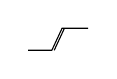
\begin{tikzpicture}\draw (0,0)--(.30,0)--(.43,.28)--(.76,.28);\draw (.33,0)--(.46,.28);\end{tikzpicture}}}}{}{author paragraph cue}{ps_134-2_037-v0019}(in a suitable sense) n-truncated homotopy types.\var{\hand{\tikz[baseline=-.4ex]{\draw (0,0)--(.30,0)--(.43,.28)--(.76,.28);\draw (.33,0)--(.46,.28);}} The third letter}{

The third letter}{author paragraph break}{ps_134-2_037-v0020}, \var{\inserted{written}}{\hand{written}}{insertion}{ps_134-2_037-v0021} \var{\inserted[typed]{in}}{in}{typed insertion}{ps_134-2_037-v0022} ans-%
wer to a number of questions in Larry Breen's response to the first two,
is of a wider scope. A large part of the letter outlines (very ske\var{\over{\unsure{t}}{tc}}{\hand{tc}}{writing over}{ps_134-2_037-v0023}hyly)
some main points of a duality program (including a cohomological formula-%
tion of ``geometric'' local and global classfield theory), which \var{\deleted{appears}}{}{deletion}{ps_134-2_037-v0024}\var{\inserted{emerged by the end of the fifties and appears}}{\hand{emerged by the end of the fifties and appears}}{insertion}{ps_134-2_037-v0025}
here for the first time in print\hand{,} \var{\deleted{and going back to the end of the fif-%
ties.}}{}{deletion}{ps_134-2_037-v0026} \var{\deleted{It}}{}{deletion}{ps_134-2_037-v0027}\var{\inserted{The later part of the letter}}{\hand{The later part of the letter}}{insertion}{ps_134-2_037-v0028} gives also some hints about the need of a framework of ``tame to-%
pology'' suitable for writing up a ``dévissage theory'' of stratified spaces,
and for \var{\xout{\unsure{dealing}}}{}{typewriter deletion}{ps_134-2_037-v0029}\var{\inserted[typed]{working}}{working}{typed insertion}{ps_134-2_037-v0030} with étale tubular neighbourhoods, for the common purpose
of coming to grips \var{\deleted{of}}{}{deletion}{ps_134-2_037-v0031}\var{\inserted{with}}{\hand{with}}{insertion}{ps_134-2_037-v0032} a suitable notion of ``fine\unsure{\hand{,}} homotopy type'' of a ``tame''
topological space or \var{\inserted{of}}{\hand{of}}{insertion}{ps_134-2_037-v0033} a scheme \var{\inserted{say}}{\hand{say}}{insertion}{ps_134-2_037-v0034}, in terms of the \var{\deleted{ordered set}}{}{deletion}{ps_134-2_037-v0035}\var{\inserted{inverse system}}{\hand{inverse system}}{insertion}{ps_134-2_037-v0036} of ``indexed
homotopy types'' corresponding to \var{\inserted{all}}{\hand{all}}{insertion}{ps_134-2_037-v0037} equisingular stratifications .

\margin{37}

%% END SOURCE ps_134-2_037
\ifnum\EditionMode=1
\psapparatusstart
\psentry{ps_134-2_037-v0001}{1}{typewriter deletion}{\xout{\unsure{1|I}}}{}{The typewriter strikes out this material; it leaves the corrected running text.}
\psentry{ps_134-2_037-v0002}{2}{typewriter deletion}{\xout{handwri}}{}{The typewriter strikes out this material; it leaves the corrected running text.}
\psentry{ps_134-2_037-v0003}{3}{deletion}{\deleted{\unsure{as it}}}{}{The author cancels this material by hand; it leaves the corrected running text.}
\psentry{ps_134-2_037-v0004}{4}{insertion}{\inserted{which}}{\hand{which}}{The handwritten insertion is incorporated at its indicated position; insertion brackets leave the running text.}
\psentry{ps_134-2_037-v0005}{5}{deletion}{\deleted{from}}{}{The author cancels this material by hand; it leaves the corrected running text.}
\psentry{ps_134-2_037-v0006}{6}{insertion}{\inserted{in}}{\hand{in}}{The handwritten insertion is incorporated at its indicated position; insertion brackets leave the running text.}
\psentry{ps_134-2_037-v0007}{7}{insertion}{\inserted{as well as \deleted{from} in}}{\hand{as well as  in}}{The handwritten insertion is incorporated at its indicated position; insertion brackets leave the running text.}
\psentry{ps_134-2_037-v0008}{8}{typewriter deletion}{\xout{copying}}{}{The typewriter strikes out this material; it leaves the corrected running text.}
\psentry{ps_134-2_037-v0009}{9}{insertion}{\inserted{that letter}}{\hand{that letter}}{The handwritten insertion is incorporated at its indicated position; insertion brackets leave the running text.}
\psentry{ps_134-2_037-v0010}{10}{writing over}{\over{u}{u}}{\hand{u}}{The superposed handwritten reading replaces the underlying reading.}
\psentry{ps_134-2_037-v0011}{11}{deletion}{\deleted{and correcting some}}{}{The author cancels this material by hand; it leaves the corrected running text.}
\psentry{ps_134-2_037-v0012}{12}{insertion}{\inserted{adding subtitles (with numbers App. 1 to App. 18), and correcting some}}{\hand{adding subtitles (with numbers App. 1 to App. 18), and correcting some}}{The handwritten insertion is incorporated at its indicated position; insertion brackets leave the running text.}
\psentry{ps_134-2_037-v0013}{13}{deletion}{\deleted{\illegible{1}}}{}{The author cancels this material by hand; it leaves the corrected running text.}
\psentry{ps_134-2_037-v0014}{14}{deletion}{\deleted{to}}{}{The author cancels this material by hand; it leaves the corrected running text.}
\psentry{ps_134-2_037-v0015}{15}{deletion}{\deleted{me}}{}{The author cancels this material by hand; it leaves the corrected running text.}
\psentry{ps_134-2_037-v0016}{16}{writing over}{\over{.}{,}}{\hand{,}}{The superposed handwritten reading replaces the underlying reading.}
\psentry{ps_134-2_037-v0017}{17}{typed insertion}{\inserted[typed]{new}}{new}{The typed insertion is incorporated at its indicated position; insertion brackets leave the running text.}
\psentry{ps_134-2_037-v0018}{18}{typewriter deletion}{\xout{which}}{}{The typewriter strikes out this material; it leaves the corrected running text.}
\psentry{ps_134-2_037-v0019}{19}{author paragraph cue}{\margin{\diagram{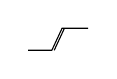
\begin{tikzpicture}\draw (0,0)--(.30,0)--(.43,.28)--(.76,.28);\draw (.33,0)--(.46,.28);\end{tikzpicture}}}}{}{The marginal stepped cue repeats the inline paragraph instruction applied before The third letter; its drawing remains in the diplomatic form.}
\psentry{ps_134-2_037-v0020}{20}{author paragraph break}{\hand{\tikz[baseline=-.4ex]{\draw (0,0)--(.30,0)--(.43,.28)--(.76,.28);\draw (.33,0)--(.46,.28);}} The third letter}{

The third letter}{The repeated stepped pen cue instructs a new paragraph at this boundary.}
\psentry{ps_134-2_037-v0021}{21}{insertion}{\inserted{written}}{\hand{written}}{The handwritten insertion is incorporated at its indicated position; insertion brackets leave the running text.}
\psentry{ps_134-2_037-v0022}{22}{typed insertion}{\inserted[typed]{in}}{in}{The typed insertion is incorporated at its indicated position; insertion brackets leave the running text.}
\psentry{ps_134-2_037-v0023}{23}{writing over}{\over{\unsure{t}}{tc}}{\hand{tc}}{The superposed handwritten reading replaces the underlying reading.}
\psentry{ps_134-2_037-v0024}{24}{deletion}{\deleted{appears}}{}{The author cancels this material by hand; it leaves the corrected running text.}
\psentry{ps_134-2_037-v0025}{25}{insertion}{\inserted{emerged by the end of the fifties and appears}}{\hand{emerged by the end of the fifties and appears}}{The handwritten insertion is incorporated at its indicated position; insertion brackets leave the running text.}
\psentry{ps_134-2_037-v0026}{26}{deletion}{\deleted{and going back to the end of the fif-%
ties.}}{}{The author cancels this material by hand; it leaves the corrected running text.}
\psentry{ps_134-2_037-v0027}{27}{deletion}{\deleted{It}}{}{The author cancels this material by hand; it leaves the corrected running text.}
\psentry{ps_134-2_037-v0028}{28}{insertion}{\inserted{The later part of the letter}}{\hand{The later part of the letter}}{The handwritten insertion is incorporated at its indicated position; insertion brackets leave the running text.}
\psentry{ps_134-2_037-v0029}{29}{typewriter deletion}{\xout{\unsure{dealing}}}{}{The typewriter strikes out this material; it leaves the corrected running text.}
\psentry{ps_134-2_037-v0030}{30}{typed insertion}{\inserted[typed]{working}}{working}{The typed insertion is incorporated at its indicated position; insertion brackets leave the running text.}
\psentry{ps_134-2_037-v0031}{31}{deletion}{\deleted{of}}{}{The author cancels this material by hand; it leaves the corrected running text.}
\psentry{ps_134-2_037-v0032}{32}{insertion}{\inserted{with}}{\hand{with}}{The handwritten insertion is incorporated at its indicated position; insertion brackets leave the running text.}
\psentry{ps_134-2_037-v0033}{33}{insertion}{\inserted{of}}{\hand{of}}{The handwritten insertion is incorporated at its indicated position; insertion brackets leave the running text.}
\psentry{ps_134-2_037-v0034}{34}{insertion}{\inserted{say}}{\hand{say}}{The handwritten insertion is incorporated at its indicated position; insertion brackets leave the running text.}
\psentry{ps_134-2_037-v0035}{35}{deletion}{\deleted{ordered set}}{}{The author cancels this material by hand; it leaves the corrected running text.}
\psentry{ps_134-2_037-v0036}{36}{insertion}{\inserted{inverse system}}{\hand{inverse system}}{The handwritten insertion is incorporated at its indicated position; insertion brackets leave the running text.}
\psentry{ps_134-2_037-v0037}{37}{insertion}{\inserted{all}}{\hand{all}}{The handwritten insertion is incorporated at its indicated position; insertion brackets leave the running text.}
\psapparatusend
\fi
\pssource{ps_134-2_038}{134-2/38}{https://grothendieck.umontpellier.fr/web/viewer.html?file=../134-2.pdf\#page=39}
\psnumber{ps_134-2_038-v0001}{1}
\psnumber{ps_134-2_038-v0002}{2}
\psnumber{ps_134-2_038-v0003}{3}
%% BEGIN SOURCE ps_134-2_038
% Pursuing Stacks (cotes 134-2 to 134-8): archive cote 134-2, site page 38 (PDF page 39).
% appendix (letters to Breen). Draft compared: ps1.tex:1174-1193.
% AI-transcribed by Claude Opus 5.5 (claude-opus-5-5, adaptive thinking, effort high), Message Batches API, batch ps1 (msgbatch_01Rv5hCaNTtUt4JHx1yqoHPL), 2026-11-12; reviewed against both supplied scan halves; see CHECK_DECISIONS.tsv.
\scanpage{134-2/38}
\mspage{\hand{23 bis}}
% NOTE: the typed text is on a slip pasted onto another typed page; text of the underlying page shows through faintly and is not transcribed

\hfill Villecun 5.2.1975\margin{--}

\margin{--} Cher Breen

\quad ....

(App.1) \quad ... Pour tout le reste de ta lettre, \ elle mériterait un lecteur
\margin{--} plus averti, \ aussi, \ pour qu'elle ne soit pas entièrement perdue au monde,
je vais l'envoyer à Illusie ! \ J'ai néanmoins
constaté\hand{,} avec intérêt\hand{,} ton intérêt à demi \unsure{rèfoulé|refoulé} pour des 2-catégories de
Picard, n-catégories et autre faune de ce genre, et ton espoir que je te
prouverai peut-être que ces animaux sont tout à fait indispensables pour
faire des maths sérieuses \ dans telle ou telle circonstance. J'ai bien \hand{peur}
que cet espoir ne soit déçu, je crois que jusqu'à maintenant on a toujours
pu s'en tirer en éludant de tels objets et l'engrenage dans lequel ils pour
-raient nous entrainer. Est-ce nécessairement une raison pour continuer à
les éluder ? Les situations où on a l'impression"d'éluder" en effet me sem-%
blent en tous cas devenir toujours plus nombreuses - \ et si on s'abstenait
de tirer une situation complexe et chargée de mystère au clair, ch\'aque
fois qu'on ne serait pas \uline{forcé} de le faire pour des raisons techniques pro-%
venant de la math déjà faite, - il y aurait sans doute beaucoup de parties
des maths aujourd'hui \var{reputées\hand{|}"sérieuses"}{reputées "sérieuses"}{author spacing cue}{ps_134-2_038-v0001} qui n'auraient jamais \var{\inserted{été}}{\hand{été}}{insertion}{ps_134-2_038-v0002} développées
(Il n'est pas dit non plus \var{que\hand{|}le monde}{que le monde}{author spacing cue}{ps_134-2_038-v0003} s'en trouverait plus mal ...). Ton
commentaire (que j'ai également entendu chez Deligne) \ que la classificati-%
on d'objets géométriques relativement merdiques se réduit finalement à des
invariants cohomologiques essentiellement "bien connus" et relativement
simples n'est pas non plus convainquant; n'est ce pas négliger la différen-%
ce entre la \uline{compréhension d'un objet géométrique}, et la détermination de
sa "classe à isomorphisme (ou équivalence...) près" ?

\margin{38}

%% END SOURCE ps_134-2_038
\ifnum\EditionMode=1
\psapparatusstart
\psentry{ps_134-2_038-v0001}{1}{author spacing cue}{reputées\hand{|}"sérieuses"}{reputées "sérieuses"}{The continuous pen stroke marks a missing space at this line boundary; apply the space while preserving its graphic in the diplomatic form.}
\psentry{ps_134-2_038-v0002}{2}{insertion}{\inserted{été}}{\hand{été}}{The handwritten insertion is incorporated at its indicated position; insertion brackets leave the running text.}
\psentry{ps_134-2_038-v0003}{3}{author spacing cue}{que\hand{|}le monde}{que le monde}{The same continuous pen stroke intersects the next line between que and le; apply the indicated word space.}
\psapparatusend
\fi
\pssource{ps_134-2_039}{134-2/39}{https://grothendieck.umontpellier.fr/web/viewer.html?file=../134-2.pdf\#page=40}
\psnumber{ps_134-2_039-v0001}{1}
\psnumber{ps_134-2_039-v0002}{2}
\psnumber{ps_134-2_039-v0003}{3}
\psnumber{ps_134-2_039-v0004}{4}
\psnumber{ps_134-2_039-v0005}{5}
\psnumber{ps_134-2_039-v0006}{6}
\psnumber{ps_134-2_039-v0007}{7}
\psnumber{ps_134-2_039-v0008}{8}
\psnumber{ps_134-2_039-v0009}{9}
\psnumber{ps_134-2_039-v0010}{10}
\psnumber{ps_134-2_039-v0011}{11}
\psnumber{ps_134-2_039-v0012}{12}
\psnumber{ps_134-2_039-v0013}{13}
\psnumber{ps_134-2_039-v0014}{14}
\psnumber{ps_134-2_039-v0015}{15}
\psnumber{ps_134-2_039-v0016}{16}
\psnumber{ps_134-2_039-v0017}{17}
\psnumber{ps_134-2_039-v0018}{18}
\psnumber{ps_134-2_039-v0019}{19}
%% BEGIN SOURCE ps_134-2_039
% Pursuing Stacks (cotes 134-2 to 134-8): archive cote 134-2, site page 39 (PDF page 40).
% appendix (letters to Breen). Draft compared: ps1.tex:1193-1197.
% AI-transcribed by Claude Opus 5.5 (claude-opus-5-5, adaptive thinking, effort high), Message Batches API, batch ps1 (msgbatch_01Rv5hCaNTtUt4JHx1yqoHPL), 2026-11-12; reviewed against both supplied scan halves; see CHECK_DECISIONS.tsv.
\scanpage{134-2/39}
\mspage{\hand{24}}

Tu me demandes des exemples "convainquants" de 2-catégories de Picard.
Voici quelques \var{\deleted{uns}}{}{deletion}{ps_134-2_039-v0001}\var{\inserted{exemples,}}{\hand{exemples,}}{insertion}{ps_134-2_039-v0002} en vrac \hand{(je ne sais s'ils seront convainquants !)}:

\margin{$\times$(22)} 1) Si L est un lien\var{\inserted{(22)}}{\hand{(22)}}{insertion}{ps_134-2_039-v0003} de centre Z sur le topos X, les \uline{gerbes liées par Z}
forment une 2-catégorie de Picard stricte, représentée par le complexe
$R\hand{\Gamma}_X(Z)$ tronqué en degré 2, dont les objets de cohomologie non triviaux
sont \unsure{Hes|les} $H^i(X,Z)$, $0 \hand{\leqslant} i \hand{\leqslant} 2$. Les \var{\over{\unsure{g}}{g}}{\hand{g}}{writing over}{ps_134-2_039-v0004}erbes liées par L forment un \uline{pseudo-2-}
\uline{torseur} sous la gerbe précédente, qui est un 2-torseur\hand{(}i.e. non vide\hand{)} sss
une certaine obstruction dans $H^3(X,Z)$ est nulle. Pour comprendre \unsure{cette}
classe de notre point de vue, il y a lieu de passer aux 2-champs derres-%
pondants: le 2-champ de\var{\xout{s}}{}{typewriter deletion}{ps_134-2_039-v0005} Picard \var{\inserted[typed]{strict,}}{strict,}{typed insertion}{ps_134-2_039-v0006} des Z-gerbes\var{\xout{\unsure{liées par Z et le 2-champ des}}}{}{typewriter deletion}{ps_134-2_039-v0007}
sur des objets variables de X, et le 2-champ des L-gerbes sur des objets
variables. Ce dernier est bel et bien un 2-torseur sous le champ précédent,
or la classification de ces \var{\xout{deux}}{}{typewriter deletion}{ps_134-2_039-v0008} 2-torseurs (à 2-équivalence près) se
fait par le $H^3(X,Z)$, \var{\xout{de façon précise}}{}{typewriter deletion}{ps_134-2_039-v0009} \hand{(}tout comme les Z-\var{\inserted{1-}}{\hand{1-}}{insertion}{ps_134-2_039-v0010}gerbes peuvent être
interpétées comme des \var{\deleted{\unsure{1}}}{}{deletion}{ps_134-2_039-v0011}torseurs sous la Z-1-\var{\over{\unsure{gerbe}}{champ}}{\hand{champ}}{writing over}{ps_134-2_039-v0012} \var{\inserted[typed]{de Picard strict,}}{de Picard strict,}{typed insertion}{ps_134-2_039-v0013} des Z-torseurs, et sont
\var{\xout{par conséquent}}{}{typewriter deletion}{ps_134-2_039-v0014} classifiées par le $H^2(X,Z)$\hand{)}. On voit déjà, bien sûr, poindre
ici l'oreille de la 3-catégorie de Picard stricte des 2-gerbes liées par Z,
ou (de façon équivalente) des 2-torseurs sous le 2-champ de Picard strict
des Z-1-gerbes; cette 3-catégorie de Picard stricte étant décrite par
$R\hand{\Gamma}_X(Z)$ tronqué en dimension 3, ayant comme invariants de cohomologie non
triviaux les $H^i(X,Z)$ $(0 \hand{\leqslant} i \hand{\leqslant} 3)$. Quant au 3-champ de Picard correspondaht,
il est décrit par une résolution injective de Z \hand{tronquée} en degré 3, alors
que le  2-champ de Picard précédent se décrivait en tronquant en degré 2.

2. Si M et N sont deux faisceaux abéliens sur X, les \uline{champs de Picard}
(NB: 1-champs !) \uline{d'invariants} M \uline{et} N forment eux-même une \var{\inserted{2-}}{\hand{2-}}{insertion}{ps_134-2_039-v0015}catégorie de
\margin{$\times$} Picard stricte, représentée  sans doute par le complexe RHom(X(M),N) \var{\inserted{(23)}}{\hand{(23)}}{insertion}{ps_134-2_039-v0016}
tronqué en \var{\xout{dimension}}{}{typewriter deletion}{ps_134-2_039-v0017} degré 2, dont les invariants de chomologie non trivi-%
aux sont donc \hand{``}le drôle de $\mathrm{Ext}^2$\hand{''} de ma lettre à Deligne, et les Honnètes
$\mathrm{Ext}^i(M,N)$  $(0 \hand{\leqslant} i \hand{\leqslant} 1)$. Les champs de Picard stricts forment une sous-2-caté%
gorie de Picard pleine, représentée par RHom(M,N) tronqué en degré 2,
d'invariants les $\mathrm{Ext}^i(M;N)$ $(0 \hand{\leqslant} i \hand{\leqslant} 2)$. Bien sûr, $\mathrm{Ext}^2$ donne les \var{\inserted{0-}}{\hand{0-}}{insertion}{ps_134-2_039-v0018}objets à
équivalence près, $\mathrm{Ext}^1$ les automorphismes à isomorphisme près de l'objet
nul, $\mathrm{Ext}^0$ les automorphismes de l'automorphisme identique audit ... Je n'ai
pas réfléchi à une bonne interprétation géométrique de la n-catégorie de
Picard associée à RHom(M,N) tronqué en degré n, et encore moins bien \var{\xout{s}}{}{typewriter deletion}{ps_134-2_039-v0019}sûr
pour RHom(X(M),N), mais sans doute il faut regarder dans la direction des
n-champs de Picard.

3. Soit G un Groupe sur X, opérant sur un faisceau abélien N. Les \uline{champs}
\uline{en} (Gr)-\uline{catégories sur} X \uline{liés par} (G,N) forment une 2-catégorie de Picard,

\margin{\hand{39}}

%% END SOURCE ps_134-2_039
\ifnum\EditionMode=1
\psapparatusstart
\psentry{ps_134-2_039-v0001}{1}{deletion}{\deleted{uns}}{}{The author cancels this material by hand; it leaves the corrected running text.}
\psentry{ps_134-2_039-v0002}{2}{insertion}{\inserted{exemples,}}{\hand{exemples,}}{The handwritten insertion is incorporated at its indicated position; insertion brackets leave the running text.}
\psentry{ps_134-2_039-v0003}{3}{insertion}{\inserted{(22)}}{\hand{(22)}}{The handwritten insertion is incorporated at its indicated position; insertion brackets leave the running text.}
\psentry{ps_134-2_039-v0004}{4}{writing over}{\over{\unsure{g}}{g}}{\hand{g}}{The superposed handwritten reading replaces the underlying reading.}
\psentry{ps_134-2_039-v0005}{5}{typewriter deletion}{\xout{s}}{}{The typewriter strikes out this material; it leaves the corrected running text.}
\psentry{ps_134-2_039-v0006}{6}{typed insertion}{\inserted[typed]{strict,}}{strict,}{The typed insertion is incorporated at its indicated position; insertion brackets leave the running text.}
\psentry{ps_134-2_039-v0007}{7}{typewriter deletion}{\xout{\unsure{liées par Z et le 2-champ des}}}{}{The typewriter strikes out this material; it leaves the corrected running text.}
\psentry{ps_134-2_039-v0008}{8}{typewriter deletion}{\xout{deux}}{}{The typewriter strikes out this material; it leaves the corrected running text.}
\psentry{ps_134-2_039-v0009}{9}{typewriter deletion}{\xout{de façon précise}}{}{The typewriter strikes out this material; it leaves the corrected running text.}
\psentry{ps_134-2_039-v0010}{10}{insertion}{\inserted{1-}}{\hand{1-}}{The handwritten insertion is incorporated at its indicated position; insertion brackets leave the running text.}
\psentry{ps_134-2_039-v0011}{11}{deletion}{\deleted{\unsure{1}}}{}{The author cancels this material by hand; it leaves the corrected running text.}
\psentry{ps_134-2_039-v0012}{12}{writing over}{\over{\unsure{gerbe}}{champ}}{\hand{champ}}{The superposed handwritten reading replaces the underlying reading.}
\psentry{ps_134-2_039-v0013}{13}{typed insertion}{\inserted[typed]{de Picard strict,}}{de Picard strict,}{The typed insertion is incorporated at its indicated position; insertion brackets leave the running text.}
\psentry{ps_134-2_039-v0014}{14}{typewriter deletion}{\xout{par conséquent}}{}{The typewriter strikes out this material; it leaves the corrected running text.}
\psentry{ps_134-2_039-v0015}{15}{insertion}{\inserted{2-}}{\hand{2-}}{The handwritten insertion is incorporated at its indicated position; insertion brackets leave the running text.}
\psentry{ps_134-2_039-v0016}{16}{insertion}{\inserted{(23)}}{\hand{(23)}}{The handwritten insertion is incorporated at its indicated position; insertion brackets leave the running text.}
\psentry{ps_134-2_039-v0017}{17}{typewriter deletion}{\xout{dimension}}{}{The typewriter strikes out this material; it leaves the corrected running text.}
\psentry{ps_134-2_039-v0018}{18}{insertion}{\inserted{0-}}{\hand{0-}}{The handwritten insertion is incorporated at its indicated position; insertion brackets leave the running text.}
\psentry{ps_134-2_039-v0019}{19}{typewriter deletion}{\xout{s}}{}{The typewriter strikes out this material; it leaves the corrected running text.}
\psapparatusend
\fi
\pssource{ps_134-2_040}{134-2/40}{https://grothendieck.umontpellier.fr/web/viewer.html?file=../134-2.pdf\#page=41}
\psnumber{ps_134-2_040-v0001}{1}
\psnumber{ps_134-2_040-v0002}{2}
\psnumber{ps_134-2_040-v0003}{3}
\psnumber{ps_134-2_040-v0004}{4}
\psnumber{ps_134-2_040-v0005}{5}
\psnumber{ps_134-2_040-v0006}{6}
\psnumber{ps_134-2_040-v0007}{7}
\psnumber{ps_134-2_040-v0008}{8}
\psnumber{ps_134-2_040-v0009}{9}
\psnumber{ps_134-2_040-v0010}{10}
\psnumber{ps_134-2_040-v0011}{11}
%% BEGIN SOURCE ps_134-2_040
% Pursuing Stacks (cotes 134-2 to 134-8): archive cote 134-2, site page 40 (PDF page 41).
% appendix (letters to Breen). Draft compared: ps1.tex:1195-1203.
% AI-transcribed by Claude Opus 5.5 (claude-opus-5-5, adaptive thinking, effort high), Message Batches API, batch ps1 (msgbatch_01Rv5hCaNTtUt4JHx1yqoHPL), 2026-11-12; reviewed against both supplied scan halves; see CHECK_DECISIONS.tsv.
\scanpage{134-2/40}
\mspage{\hand{25}}

dont les invariants sont $H^3(B_G \text{ mod } X,N)$, $H^2(B_G \text{ mod } X,N)$, et $Z^1(G,N)$ (groupe
des 1-cocyles de $G$ à coéfficients dans $N$)- je te laisse le soin de deviner
quel est le complexe tronqué qui le décrit ! J'ai écrit il y a quelques
mois à Deligne à ce sujet, et l'ai prié de t'envoyer une copie de \var{\xout{envoyer}}{}{typewriter deletion}{ps_134-2_040-v0001}
la lettre.

4) Soit $X$ un topos localement annelé, on peut considérer les \uline{Algèbres
d'Azumaya sur} $X$ (i.e. les Algèbres localement isomorphes à une alg. de
matrices d'ordre $n$, $n \hand{\geq} 1$) comme les objets d'une 2-catégorie de Picard,
où la catégorie $\underline{\mathrm{Hom}}(A,B)$, pour $A$ et $B$ des Algèbres d'Azumaya, est la caté-%
gorie des ``trivialisations'' de $A^o\otimes B$, i.e. des couples $(E,\hand{\phi})$, $E$ un Module
localement libre et $\hand{\phi}$ un isomorphisme $\underline{\mathrm{End}}(E)\simeq A^o\otimes B$. Il faut travailler
un peu pour définir les accouplements\var{\xout{x}}{}{typewriter deletion}{ps_134-2_040-v0002} $\underline{\mathrm{Hom}}(A,B)\mathrm{x}\underline{\mathrm{Hom}}(B,C)\hand{\to}\underline{\mathrm{Hom}}(A,C)$; l'opé-%
ration $\otimes$ dans la 2-catégorie de Picard à construire est bien sûr le produit
tensoriel d'Algèbres, et l'opération ``puissance $-1$'' est le passage à l'al-%
gèbre opposée. On \unsure{vérfie|vérifie}\var{\xout{,x\allowbreak{}x\allowbreak{} passant aux champs correspondant, qui sont}}{}{typewriter deletion}{ps_134-2_040-v0003} qu'en
associant à toute Algèbre d'Azumaya la 1-gerbe de ses trivialisations, on
trouve un 2-$\otimes$-foncteur de la 2-catégorie de Picard (dite ``de Brauer'') dans
celle des 1-gerbes liées par $\underline{G}_m$ , qui est 2-fidèle. Les invariants de
la première sont donc les groupes $H^2(X,\underline{G}_m)_{Br}$ , $H^1(X,\underline{H}_m)$ et $H^o(X,\underline{G}_m)$ , où
dans le premier terme l'indice Br désigne le sous-groupe du $H^2$ formé des
classes de cohomologie provenant d'Algèbres d'Azumaya. On aurait envie
de parler du 2-champ de Picard des Algèbres d'Azumaya sur des objets variab
les de $X$, mais c'est bien une 2-catégorie de Picard fibrée sur $X$, mais pas
tout à fait un 2-champ (whatever that means), sans doute - la condition de
2-recollement (whatever that means) ne doit pas être satisfaite - sinon il
n'y aurait pas d'indice Br au $H^2$ ...
\var{\margin{\(\uparrow\) espace \(\downarrow\)}}{\par\medskip}{author spacing cue}{ps_134-2_040-v0004}

\var{\inserted{(App.2)}}{\hand{(App.2)}}{insertion}{ps_134-2_040-v0005} La considération des $n$-catégories de Picard \var{\inserted[typed]{strictes}}{strictes}{typed insertion}{ps_134-2_040-v0006} (qui s'imposent à nous pas
à pas dans un contexte essentiellement ``commutatif'') me semblent la clef du
passage de l'algèbre homologique ordinaire (``commutative''), en termes de
complexes, à une algèbre homologique non commutative, du fait qu'elles
donnent une interprétation géométrique correcte des ``complexes tronqués à
l'ordre $n$'' \var{\inserted{(en tant qu'objets de catégories dérivées)}}{\hand{(en tant qu'objets de catégories dérivées)}}{insertion}{ps_134-2_040-v0007}, donc, essentiellement (par passage à la limite sur $n$) des
complexes tout courts. L'idée naive qui se présente est alors que les
``complexes non commutatifs'' (qui seraient les objets-fantômes d'une algèbre
homologique non commutative) sont peut-être ce qui reste des $n$-catégories
de Picard (strictes) quand on oublie \var{leut caractère}{leur caractère}{slip corrected}{ps_134-2_040-v0008} additif, i.e. leur
structure de Picard - c'est à dire qu'on ne retient que la $n$-catégorie !
\var{\inserted{(Quand on se place sur un topos $X$, on s'intéresse donc aux $n$-champs sur $X$...)}}{\hand{(Quand on se place sur un topos $X$, on s'intéresse donc aux $n$-champs sur $X$...)}}{insertion}{ps_134-2_040-v0009}
A vrai dire, cette idée est venue d'abord d'une autre direction, quand il
s'est agi en géométrie algébrique de démontrer des \uline{\var{\deleted{formules}}{}{deletion}{ps_134-2_040-v0010}\var{\inserted{théorèmes}}{\hand{théorèmes}}{insertion}{ps_134-2_040-v0011} de Lefschetz}

\margin{\hand{40}}

%% END SOURCE ps_134-2_040
\ifnum\EditionMode=1
\psapparatusstart
\psentry{ps_134-2_040-v0001}{1}{typewriter deletion}{\xout{envoyer}}{}{The typewriter strikes out this material; it leaves the corrected running text.}
\psentry{ps_134-2_040-v0002}{2}{typewriter deletion}{\xout{x}}{}{The typewriter strikes out this material; it leaves the corrected running text.}
\psentry{ps_134-2_040-v0003}{3}{typewriter deletion}{\xout{,x\allowbreak{}x\allowbreak{} passant aux champs correspondant, qui sont}}{}{The typewriter strikes out this material; it leaves the corrected running text.}
\psentry{ps_134-2_040-v0004}{4}{author spacing cue}{\margin{\(\uparrow\) espace \(\downarrow\)}}{\par\medskip}{Apply the opposed arrows and espace instruction as additional paragraph separation before App.2; retain the graphic diplomatically.}
\psentry{ps_134-2_040-v0005}{5}{insertion}{\inserted{(App.2)}}{\hand{(App.2)}}{The handwritten insertion is incorporated at its indicated position; insertion brackets leave the running text.}
\psentry{ps_134-2_040-v0006}{6}{typed insertion}{\inserted[typed]{strictes}}{strictes}{The typed insertion is incorporated at its indicated position; insertion brackets leave the running text.}
\psentry{ps_134-2_040-v0007}{7}{insertion}{\inserted{(en tant qu'objets de catégories dérivées)}}{\hand{(en tant qu'objets de catégories dérivées)}}{The handwritten insertion is incorporated at its indicated position; insertion brackets leave the running text.}
\psentry{ps_134-2_040-v0008}{8}{slip corrected}{leut caractère}{leur caractère}{One-off t for r; leur is correctly typed in the following clause referring to the same Picard structure.}
\psentry{ps_134-2_040-v0009}{9}{insertion}{\inserted{(Quand on se place sur un topos $X$, on s'intéresse donc aux $n$-champs sur $X$...)}}{\hand{(Quand on se place sur un topos $X$, on s'intéresse donc aux $n$-champs sur $X$...)}}{The handwritten insertion is incorporated at its indicated position; insertion brackets leave the running text.}
\psentry{ps_134-2_040-v0010}{10}{deletion}{\deleted{formules}}{}{The author cancels this material by hand; it leaves the corrected running text.}
\psentry{ps_134-2_040-v0011}{11}{insertion}{\inserted{théorèmes}}{\hand{théorèmes}}{The handwritten insertion is incorporated at its indicated position; insertion brackets leave the running text.}
\psapparatusend
\fi
\pssource{ps_134-2_041}{134-2/41}{https://grothendieck.umontpellier.fr/web/viewer.html?file=../134-2.pdf\#page=42}
\psnumber{ps_134-2_041-v0001}{1}
\psnumber{ps_134-2_041-v0002}{2}
\psnumber{ps_134-2_041-v0003}{3}
\psnumber{ps_134-2_041-v0004}{4}
\psnumber{ps_134-2_041-v0005}{5}
\psnumber{ps_134-2_041-v0006}{6}
\psnumber{ps_134-2_041-v0007}{7}
\psnumber{ps_134-2_041-v0008}{8}
\psnumber{ps_134-2_041-v0009}{9}
\psnumber{ps_134-2_041-v0010}{10}
\psnumber{ps_134-2_041-v0011}{11}
\psnumber{ps_134-2_041-v0012}{12}
\psnumber{ps_134-2_041-v0013}{13}
\psnumber{ps_134-2_041-v0014}{14}
\psnumber{ps_134-2_041-v0015}{15}
\psnumber{ps_134-2_041-v0016}{16}
%% BEGIN SOURCE ps_134-2_041
% Pursuing Stacks (cotes 134-2 to 134-8): archive cote 134-2, site page 41 (PDF page 42).
% appendix (letters to Breen). Draft compared: ps1.tex:1203-1205.
% AI-transcribed by Claude Opus 5.5 (claude-opus-5-5, adaptive thinking, effort high), Message Batches API, batch ps1 (msgbatch_01Rv5hCaNTtUt4JHx1yqoHPL), 2026-11-12; reviewed against both supplied scan halves; see CHECK_DECISIONS.tsv.
\scanpage{134-2/41}
\mspage{\hand{26}}

à coéfficients discrets \var{\inserted{en cohomologie étale}}{\hand{en cohomologie étale}}{insertion}{ps_134-2_041-v0001}, dans le cas d'une variété projective disons et
de toute section hyperplane, ou d'une variété quasi-projective et de presque
toute section hyperplane (pour ne mentionner que le cas global le plus sim-%
ple), sous les hypothèses de profondeur \var{\inserted[typed]{cohomologique}}{cohomologique}{typed insertion}{ps_134-2_041-v0002} ``les plus naturelles'' (en fait,
essenti\var{\over{\unsure{a}}{e}}{\hand{e}}{writing over}{ps_134-2_041-v0003}llement des conditions néc. et suff. de validité dudit théorème).
Dans le cas commutatif, les techniques de dualité nous suggèrent très clai-%
rement quels sont les meilleurs énoncés possibles, cf. l'exposé de Mme \var{Ray-%
naus}{Ray-%
naud}{slip corrected}{ps_134-2_041-v0004} dans SGA 2. Mais ces techniques ne valent qu'en se restreignant à des
coéfficients premiers aux caractéristiques, alors que des démonstrations
directes plus géométriques (développées dans SGA 2 av\var{\over{\unsure{e}}{a}}{\hand{a}}{writing over}{ps_134-2_041-v0005}nt le développement
du formalisme de la cohomologie étale) donnaient des résultats très voisins
\margin{$\pi_0,\pi_1$}pour le H$^0$ et le H$^1$ (ou le \var{\inserted{$\pi_0$ et le}}{\hand{$\pi_0$ et le}}{insertion}{ps_134-2_041-v0006} $\hand{\pi}_1$ , si on préfère) sans telles restrictions,
du moins dans le cas propre (i.e. projectif, au lieu de quasi-projectif).
En fai\hand{t}, ce sont \var{\deleted{en fait}}{}{deletion}{ps_134-2_041-v0007} \var{\over{\unsure{d}}{l}}{\hand{l}}{writing over}{ps_134-2_041-v0008}es ``résultats les meilleurs possibles'' eux-%
mêmes, énoncés comme conjectures dans SGA 2 dans l'exposé cité de Mme \var{\over{\unsure{R}}{R}}{\hand{R}}{writing over}{ps_134-2_041-v0009}ay-%
naud, qui sont démontrés ultérieurement par elle dans sa thèse. Ce qui est
remarquable de notre point de vue, c'est que les énoncés les plus forts se
présentent le plus naturellement sous forme d'énoncés sur des \var{\inserted{1-}}{\hand{1-}}{insertion}{ps_134-2_041-v0010}\uline{champs} sur
le site étale de la variété algébrique considérée - la notion de ``profon-%
deur $\hand{\geq}$ i'' (pour i=\var{\over{1}{1}}{\hand{1}}{writing over}{ps_134-2_041-v0011},2,3) s'énonçant aussi le plus naturellement en termes
de champs. Non seulement cela, mais alors même qu'on voudrait ignorer la
notion technique de champ et travailler exclusivement en termes de H$^0$ et
H$^1$en utilisant à bloc le formalisme \var{\inserted{cohomologique non commutatif}}{\hand{cohomologique non commutatif}}{insertion}{ps_134-2_041-v0012} de Giraud, pour démontrer disons un
théorème de bijectivité $\hand{\pi}_1$(Y)$\hand{\to}\hand{\pi}_1$(X) (ce qui est le résultat le plus pro-%
fond établi dans la thèse de Mme Raynaud), il semble bien qu'on n'y arrive\hand{\unsure{''}}
\var{\xout{xxxx}}{}{typewriter deletion}{ps_134-2_041-v0013} pas, faute \var{\xout{dxxxxixxa}}{}{typewriter deletion}{ps_134-2_041-v0014} à ce formalisme d'avoir la souplesse nécessaire\hand{.}
En fait, il faut utiliser comme ingrédients techniques, de façon essentielle\hand{,}
les trois théorèmes suivants directement pour les 1-champs ``de torsion''
(i.e. où les faisceaux en groupes d'automorphismes sont de ind-torsion):
a) théorème de changement de base pour un morphisme propre, b) théorème de
changement de base par un morphisme lisse  c) théorème de \var{\xout{xhanx}}{}{typewriter deletion}{ps_134-2_041-v0015} ``propreté
cohomologique générique'' pour un morphisme de type fini f: X$\hand{\to}$S, S intègre
(disant que l'on peut trouver dans S un ouvert U$\neq\emptyset$ tel que pour \uline{tout} change
ment de base S'$\hand{\to}$ S se factorisant par u, la formule de changement de base
est vraie). \hand{(}Pour b) et c), il faut faire des hypothèses que les \var{faisdeaux}{faisceaux}{slip corrected}{ps_134-2_041-v0016}
d'automorphismes sont premiers aux cara\unsure{ct}érisitques, et dans c) une hypothè
se de constructtibilité sur ces faisceaux - mais b) et c) ne servent que
dans la version ``générique'' du th. de Lefschetz.\hand{)} C'est avec en vue de telle\hand{s}
applications que Giraud a pris la peine dans son bouquin (si je ne me trompe\hand{)}
de demontrer a)\hand{,} b) (et c) ?) dans le contexte des 1-champs et de leurs

\margin{\hand{41}}

%% END SOURCE ps_134-2_041
\ifnum\EditionMode=1
\psapparatusstart
\psentry{ps_134-2_041-v0001}{1}{insertion}{\inserted{en cohomologie étale}}{\hand{en cohomologie étale}}{The handwritten insertion is incorporated at its indicated position; insertion brackets leave the running text.}
\psentry{ps_134-2_041-v0002}{2}{typed insertion}{\inserted[typed]{cohomologique}}{cohomologique}{The typed insertion is incorporated at its indicated position; insertion brackets leave the running text.}
\psentry{ps_134-2_041-v0003}{3}{writing over}{\over{\unsure{a}}{e}}{\hand{e}}{The superposed handwritten reading replaces the underlying reading.}
\psentry{ps_134-2_041-v0004}{4}{slip corrected}{Ray-%
naus}{Ray-%
naud}{One-off final s for d; Raynaud appears twice later on this same checked page.}
\psentry{ps_134-2_041-v0005}{5}{writing over}{\over{\unsure{e}}{a}}{\hand{a}}{The superposed handwritten reading replaces the underlying reading.}
\psentry{ps_134-2_041-v0006}{6}{insertion}{\inserted{$\pi_0$ et le}}{\hand{$\pi_0$ et le}}{The handwritten insertion is incorporated at its indicated position; insertion brackets leave the running text.}
\psentry{ps_134-2_041-v0007}{7}{deletion}{\deleted{en fait}}{}{The author cancels this material by hand; it leaves the corrected running text.}
\psentry{ps_134-2_041-v0008}{8}{writing over}{\over{\unsure{d}}{l}}{\hand{l}}{The superposed handwritten reading replaces the underlying reading.}
\psentry{ps_134-2_041-v0009}{9}{writing over}{\over{\unsure{R}}{R}}{\hand{R}}{The superposed handwritten reading replaces the underlying reading.}
\psentry{ps_134-2_041-v0010}{10}{insertion}{\inserted{1-}}{\hand{1-}}{The handwritten insertion is incorporated at its indicated position; insertion brackets leave the running text.}
\psentry{ps_134-2_041-v0011}{11}{writing over}{\over{1}{1}}{\hand{1}}{The superposed handwritten reading replaces the underlying reading.}
\psentry{ps_134-2_041-v0012}{12}{insertion}{\inserted{cohomologique non commutatif}}{\hand{cohomologique non commutatif}}{The handwritten insertion is incorporated at its indicated position; insertion brackets leave the running text.}
\psentry{ps_134-2_041-v0013}{13}{typewriter deletion}{\xout{xxxx}}{}{The typewriter strikes out this material; it leaves the corrected running text.}
\psentry{ps_134-2_041-v0014}{14}{typewriter deletion}{\xout{dxxxxixxa}}{}{The typewriter strikes out this material; it leaves the corrected running text.}
\psentry{ps_134-2_041-v0015}{15}{typewriter deletion}{\xout{xhanx}}{}{The typewriter strikes out this material; it leaves the corrected running text.}
\psentry{ps_134-2_041-v0016}{16}{slip corrected}{faisdeaux}{faisceaux}{One-off d for c; faisceaux is correctly typed in the following constructibility qualification on this checked page.}
\psapparatusend
\fi
\pssource{ps_134-2_042}{134-2/42}{https://grothendieck.umontpellier.fr/web/viewer.html?file=../134-2.pdf\#page=43}
\psnumber{ps_134-2_042-v0001}{1}
\psnumber{ps_134-2_042-v0002}{2}
\psnumber{ps_134-2_042-v0003}{3}
\psnumber{ps_134-2_042-v0004}{4}
\psnumber{ps_134-2_042-v0005}{5}
\psnumber{ps_134-2_042-v0006}{6}
\psnumber{ps_134-2_042-v0007}{7}
\psnumber{ps_134-2_042-v0008}{8}
\psnumber{ps_134-2_042-v0009}{9}
\psnumber{ps_134-2_042-v0010}{10}
\psnumber{ps_134-2_042-v0011}{11}
\psnumber{ps_134-2_042-v0012}{12}
\psnumber{ps_134-2_042-v0013}{13}
\psnumber{ps_134-2_042-v0014}{14}
\psnumber{ps_134-2_042-v0015}{15}
%% BEGIN SOURCE ps_134-2_042
% Pursuing Stacks (cotes 134-2 to 134-8): archive cote 134-2, site page 42 (PDF page 43).
% appendix (letters to Breen). Draft compared: ps1.tex:1203-1212.
% AI-transcribed by Claude Opus 5.5 (claude-opus-5-5, adaptive thinking, effort high), Message Batches API, batch ps1 (msgbatch_01Rv5hCaNTtUt4JHx1yqoHPL), 2026-11-12; reviewed against both supplied scan halves; see CHECK_DECISIONS.tsv.
\scanpage{134-2/42}
\mspage{\hand{27}}

images directes et inverses. Mais du même coup il devient clair que le
\var{contexte\hand{|}}{contexte }{author spacing cue}{ps_134-2_042-v0001}``\var{naturel''\hand{/}des}{naturel'' des}{author spacing cue}{ps_134-2_042-v0002} théorèmes de changement de base en c\unsure{\var{\over[typed]{b}{o}}{o}{typewriter overwriting}{ps_134-2_042-v0003}}homologie étale,
des théorèmes \var{\inserted[typed]{du type}}{du type}{typed insertion}{ps_134-2_042-v0004} de Lefschetz (dits ``faibles'') sur les ``sections hyperplanes'',
tout comme \var{\inserted[typed]{de}}{de}{typed insertion}{ps_134-2_042-v0005} la notion de profondeur qui y joue un rôle crucial, \hand{doit} \var{\inserted{être}}{\hand{être}}{insertion}{ps_134-2_042-v0006} celui
des n-champs. Et que le développement hypothétique de ce contexte\var{\deleted{,}}{}{deletion}{ps_134-2_042-v0007} ne ris-%
que pas de se réduire à une jonglerie purement formelle et absolument bor-%
délique avec du ``general nonsense'', mais qu'on se trouvera aussitôt confron-%
té à des tests ``d'utilisabilité'' aussi sérieux que la démonstration des
théorèmes de changement de base et ceux du type de Lefschetz (qui même
dans le contexte commutatif ne sont pas piqués de vers ...). \hand{Idem pour
variantes analytiques complexes etc.}

Je ne sais si ces commentaires te ``passent par dessus la tête'' à ton
tour, ni si elles te donnent l'impression \var{qu'il\hand{/}}{qu'il }{author spacing cue}{ps_134-2_042-v0008}\var{y\hand{/}aurait}{y aurait}{author spacing cue}{ps_134-2_042-v0009} peut-être des cho-%
ses intéressantes à tirer au clair. Si cela t'intéresse, je pourrais expli-%
citer sous forme un peu plus systématique quelques ingrédients d'une hypo-%
thétique algèbre homologique non commutative et les liens de celle-ci à
l'algèbre homologique commutative. Plus mystérieux pour moi (et pour cause,
vu mon ignorance en homotopie) seraient les relations entre celle-là et
l'algèbre homotopique, I.e. les structures semi-simpliciales, et je n'ai
que des commentaires assez vagues à faire en ce sens\hand{(*)}.Par ailleurs, je te
rappelle que même l'algèbre homologique \var{\xout{\illegible{1}}}{}{typewriter deletion}{ps_134-2_042-v0010} commutative n'est pas, il s'en
faut, dans un état satisfaisant, pour autant que je sache, vu qu'on ne sait
\margin{(24)} toujours pas quelle est la ``bonne'' notion de catégorie triangulée\hand{\unsure{(*)}}. Or il me
semble bien clair que ce n'est pas une question purement académique - même
si on a pu se passer de le savoir jusqu'ici (en se bornant comme Monsieur
Jourdain à ``faire de la \unsure{prosé|prose} sans le savoir'' - en travaillant sur des
catégories de complexes, éventuellement filtrés, sans trop se demander quel
-les structures il y a sur ces catégories ...).

Bien cordialement à toi

\hand{A Grothendieck}

\margin{(App.3)} \hand{(*) P.S.} Réflexion faite, j'ai quand même envie de te mettre un peu en ap-%
pétit, en faisant ces ``quelques commentaires assez vagues\hand{''}. Il s'agit du
yoga qu'une \var{\inserted{\deleted{\illegible{1}} (petite)}}{\hand{ (petite)}}{insertion}{ps_134-2_042-v0011} n-catégorie \var{\inserted{en groupoïdes}}{\hand{en groupoïdes}}{insertion}{ps_134-2_042-v0012} (à n-équivalence près\unsure{\hand{)}} \var{\deleted{\unsure{``}est}}{}{deletion}{ps_134-2_042-v0013} \var{\inserted{``est}}{\hand{``est}}{insertion}{ps_134-2_042-v0014} essentiellement la même
chose'' qu'un ensemble semi-simplicial pris à homotopie près et où on négli-%
ge les \hand{$\pi$}$_i$ pour i \hand{$\geq$} n+1 (où, si tu préfères,``où on a tué les groupes d'homo-%
topie en dimension \hand{$\geq$}n+1''). Voici des éléments heuristiques pour ce yoga.
Si K. est un ensemble simplicial (il peut être prudent de le prendre de
Kan) on lui associe une n-catégorie \var{\xout{K}}{}{typewriter deletion}{ps_134-2_042-v0015} C$_n$(K.), dont les 0-objets sont les

\margin{\hand{42}}

%% END SOURCE ps_134-2_042
\ifnum\EditionMode=1
\psapparatusstart
\psentry{ps_134-2_042-v0001}{1}{author spacing cue}{contexte\hand{|}}{contexte }{Apply the pen separation stroke as a word space while preserving the graphic in the diplomatic form.}
\psentry{ps_134-2_042-v0002}{2}{author spacing cue}{naturel''\hand{/}des}{naturel'' des}{Apply the pen separation stroke as a word space while preserving the graphic in the diplomatic form.}
\psentry{ps_134-2_042-v0003}{3}{typewriter overwriting}{\over[typed]{b}{o}}{o}{The superposed typed reading replaces the underlying reading.}
\psentry{ps_134-2_042-v0004}{4}{typed insertion}{\inserted[typed]{du type}}{du type}{The typed insertion is incorporated at its indicated position; insertion brackets leave the running text.}
\psentry{ps_134-2_042-v0005}{5}{typed insertion}{\inserted[typed]{de}}{de}{The typed insertion is incorporated at its indicated position; insertion brackets leave the running text.}
\psentry{ps_134-2_042-v0006}{6}{insertion}{\inserted{être}}{\hand{être}}{The handwritten insertion is incorporated at its indicated position; insertion brackets leave the running text.}
\psentry{ps_134-2_042-v0007}{7}{deletion}{\deleted{,}}{}{The author cancels this material by hand; it leaves the corrected running text.}
\psentry{ps_134-2_042-v0008}{8}{author spacing cue}{qu'il\hand{/}}{qu'il }{Apply the pen separation stroke as a word space while preserving the graphic in the diplomatic form.}
\psentry{ps_134-2_042-v0009}{9}{author spacing cue}{y\hand{/}aurait}{y aurait}{Apply the pen separation stroke as a word space while preserving the graphic in the diplomatic form.}
\psentry{ps_134-2_042-v0010}{10}{typewriter deletion}{\xout{\illegible{1}}}{}{The typewriter strikes out this material; it leaves the corrected running text.}
\psentry{ps_134-2_042-v0011}{11}{insertion}{\inserted{\deleted{\illegible{1}} (petite)}}{\hand{ (petite)}}{The handwritten insertion is incorporated at its indicated position; insertion brackets leave the running text.}
\psentry{ps_134-2_042-v0012}{12}{insertion}{\inserted{en groupoïdes}}{\hand{en groupoïdes}}{The handwritten insertion is incorporated at its indicated position; insertion brackets leave the running text.}
\psentry{ps_134-2_042-v0013}{13}{deletion}{\deleted{\unsure{``}est}}{}{The author cancels this material by hand; it leaves the corrected running text.}
\psentry{ps_134-2_042-v0014}{14}{insertion}{\inserted{``est}}{\hand{``est}}{The handwritten insertion is incorporated at its indicated position; insertion brackets leave the running text.}
\psentry{ps_134-2_042-v0015}{15}{typewriter deletion}{\xout{K}}{}{The typewriter strikes out this material; it leaves the corrected running text.}
\psapparatusend
\fi
\pssource{ps_134-2_043}{134-2/43}{https://grothendieck.umontpellier.fr/web/viewer.html?file=../134-2.pdf\#page=44}
\psnumber{ps_134-2_043-v0001}{1}
\psnumber{ps_134-2_043-v0002}{2}
\psnumber{ps_134-2_043-v0003}{3}
\psnumber{ps_134-2_043-v0004}{4}
\psnumber{ps_134-2_043-v0005}{5}
\psnumber{ps_134-2_043-v0006}{6}
\psnumber{ps_134-2_043-v0007}{7}
\psnumber{ps_134-2_043-v0008}{8}
\psnumber{ps_134-2_043-v0009}{9}
\psnumber{ps_134-2_043-v0010}{10}
\psnumber{ps_134-2_043-v0011}{11}
\psnumber{ps_134-2_043-v0012}{12}
\psnumber{ps_134-2_043-v0013}{13}
\psnumber{ps_134-2_043-v0014}{14}
\psnumber{ps_134-2_043-v0015}{15}
\psnumber{ps_134-2_043-v0016}{16}
\psnumber{ps_134-2_043-v0017}{17}
%% BEGIN SOURCE ps_134-2_043
% Pursuing Stacks (cotes 134-2 to 134-8): archive cote 134-2, site page 43 (PDF page 44).
% appendix (letters to Breen). Draft compared: ps1.tex:1210-1212.
% AI-transcribed by Claude Opus 5.5 (claude-opus-5-5, adaptive thinking, effort high), Message Batches API, batch ps1 (msgbatch_01Rv5hCaNTtUt4JHx1yqoHPL), 2026-11-12; reviewed against both supplied scan halves; see CHECK_DECISIONS.tsv.
\scanpage{134-2/43}
\mspage{\hand{28}}

O-simplexes, les 1-objets sont les chemins \var{\xout{entre}}{}{typewriter deletion}{ps_134-2_043-v0001} (ou homotopies) entre
O-simplexes, les 2-objets sont les homotopies entre chemins (à extrémités fi-%
xées) etc. Pour les n-objets, cependant, on ne prend pas les homotopies
entre homotopies de fourbis, mais classes d'équivalence \var{\xout{\unsure{entre}}}{}{typewriter deletion}{ps_134-2_043-v0002}\hand{d'}homotopies
(modulo la relation d'homotopie) entre homotopies. La composition des
i-objets ($i\hand{\geq}1$) se définit de façon évidente, on notera qu'elle n'est pas
strictement associative, mais associative modulo homotopie. Donc la n-caté-%
gorie qu'on obtient n'est pas"stricte" - et on prévoit pas mal d'emmerdement
pour définir de façon raisonnable une n-catégorie pas stricte (dans la
\var{\unsure{déscription}\hand{/}des}{\unsure{déscription} des}{author spacing cue}{ps_134-2_043-v0003} compatibilités \var{\xout{entre}}{}{typewriter deletion}{ps_134-2_043-v0004} pour les "données d'associativité\hand{"}). La
mise sur pied du yoga qui suit pourrait constituer un fil d'\hand{A}riane pour la
définition en forme des \var{n-c\hand{\tikz[baseline=-.4ex]{\draw (0,0) .. controls (.06,-.01) and (.13,.02) .. (.22,.09);}}atégories}{n-catégories}{author joining cue}{ps_134-2_043-v0005} (pas strictes), les n-foncteurs entre
elles (pas non plus stricts, et pour cause), les n-équivalences etc, au
même t\var{\over[typed]{u}{i}}{i}{typewriter overwriting}{ps_134-2_043-v0006}tre que le yoga initial "une n-catégorie est une catégorie ou les
Hom et leurs accouplements \var{\inserted[typed]{de composition}}{de composition}{typed insertion}{ps_134-2_043-v0007} sont des(n-1)-catégories et des accouplements
entre telles". Cette n-catégorie \var{\inserted{$C_n(K.)$}}{\hand{$C_n(K.)$}}{insertion}{ps_134-2_043-v0008} dépend fonctoriellement de $K.$ , tout
morphisme simplicial $K. \hand{\to} K'.$ définit un n-foncteur $C_n(K.)\hand{\to}C_n(K'.)$; en
fait, cela doit en dépendre même n-fonctoriellement, vu qu'on voit (en s'in%
spirant de ce qui précède et l'appliquant à des ensembles semi-simpliciaux
de la forme $Hom.(K.,K'.)$) que les ensembles semi-simpliciaux forment eux-%
mêmes \var{\xout{une}}{}{typewriter deletion}{ps_134-2_043-v0009}\var{\inserted[typed]{les O-objets d'une}}{les O-objets d'une}{typed insertion}{ps_134-2_043-v0010} n-catégorie, quel que soit $N$ ...

En fait, $C_n(K.)$ est un\var{\xout{e}}{}{typewriter deletion}{ps_134-2_043-v0011} n-groupoïde, i.e. une n-catégorie où toute
i-fléche ($1\hand{\leq} i\hand{\leq} n$) (= i-objet) est une "équivalence" i.e. admet un quasi-%
inverse (donc un inverse si la n-catégorie est"réduite"). Si C est une
telle \var{n-c\hand{\tikz[baseline=-.4ex]{\draw (0,0) .. controls (.06,-.01) and (.13,.02) .. (.22,.09);}}atégorie i.e.}{n-catégorie i.e.}{author joining cue}{ps_134-2_043-v0012} un n-groupoïde, et x un O-objet de C, il s'impose
de désigner par $\hand{\pi_{\unsure{i|2}}}(C,x)$ ($O\hand{\leq} i\hand{\leq} n$) successivement: l'ensemble des classes
de O-objets à équivalence près (c'est un vulgaire ensemble), l'ensemble des
classes à équivalence près de 1-objets\hand{(}ou 1-flèches\hand{)} $x \hand{\to} x$ (c'est un groupe,
pas nécessairement commutatif), l'ensemble des \var{\inserted[typed]{classes mod équivalence des}}{classes mod équivalence des}{typed insertion}{ps_134-2_043-v0013} 2-flèches $1_x \hand{\to} 1_x$ , où $1_x$
est la 1-flèche identique de x (c'est un groupe commutatif $\hand{\pi}_2(C,x)$, ainsi
que les groupes qui vont suivre), l'ensemble des classes mod équivalence
de 3-flèches $1_{1_x} \hand{\longrightarrow} 1_{1_x}$ , etc. Ces groupes forment, comme de juste, des
"systèmes \var{loc aux}{locaux}{slip corrected}{ps_134-2_043-v0014}" sur l'ensemble des O-objets de C, et modulo le grain de
sel habituel, \var{\inserted[typed]{les $\hand{\pi}_i(C,x)$}}{les $\hand{\pi}_i(C,x)$}{typed insertion}{ps_134-2_043-v0015} ne dépendent que de la"composante connexe" du O-objet x i.e.
de sa classe modulo équivalence de O-objets. Ceci dit, si C est de la form\unsure{e}
$C_n(K.)$, il résulte pratiquement des définitions que \var{\xout{les}}{}{typewriter deletion}{ps_134-2_043-v0016} l'on a des isomor%
phismes canoniques $\hand{\pi}_i(K.,x)\hand{\simeq}\hand{\pi}_i(C_n(K.))$ pour $0\hand{\leq} i\hand{\leq} n$, qui pour x variable
peuvent s'interpréter comme des \var{\over{\illegible{1}}{i}}{\hand{i}}{writing over}{ps_134-2_043-v0017}somorphismes de systèmes locaux. Il s'en-%
suit que pour une application semi-simpliciale \hand{$f$}:$K. \hand{\to} K.'$, le n-foncteur
correspondant $C_n(K.) \hand{\to} C_n(K.')$ est une n-équivalence sss f induit un iso-%

\margin{\hand{43}}

%% END SOURCE ps_134-2_043
\ifnum\EditionMode=1
\psapparatusstart
\psentry{ps_134-2_043-v0001}{1}{typewriter deletion}{\xout{entre}}{}{The typewriter strikes out this material; it leaves the corrected running text.}
\psentry{ps_134-2_043-v0002}{2}{typewriter deletion}{\xout{\unsure{entre}}}{}{The typewriter strikes out this material; it leaves the corrected running text.}
\psentry{ps_134-2_043-v0003}{3}{author spacing cue}{\unsure{déscription}\hand{/}des}{\unsure{déscription} des}{The pen separator instructs a word space before des; the overtyped preceding word remains doubtful.}
\psentry{ps_134-2_043-v0004}{4}{typewriter deletion}{\xout{entre}}{}{The typewriter strikes out this material; it leaves the corrected running text.}
\psentry{ps_134-2_043-v0005}{5}{author joining cue}{n-c\hand{\tikz[baseline=-.4ex]{\draw (0,0) .. controls (.06,-.01) and (.13,.02) .. (.22,.09);}}atégories}{n-catégories}{Apply the curved pen mark joining the separated parts of the typed word; retain its graphic diplomatically.}
\psentry{ps_134-2_043-v0006}{6}{typewriter overwriting}{\over[typed]{u}{i}}{i}{The superposed typed reading replaces the underlying reading.}
\psentry{ps_134-2_043-v0007}{7}{typed insertion}{\inserted[typed]{de composition}}{de composition}{The typed insertion is incorporated at its indicated position; insertion brackets leave the running text.}
\psentry{ps_134-2_043-v0008}{8}{insertion}{\inserted{$C_n(K.)$}}{\hand{$C_n(K.)$}}{The handwritten insertion is incorporated at its indicated position; insertion brackets leave the running text.}
\psentry{ps_134-2_043-v0009}{9}{typewriter deletion}{\xout{une}}{}{The typewriter strikes out this material; it leaves the corrected running text.}
\psentry{ps_134-2_043-v0010}{10}{typed insertion}{\inserted[typed]{les O-objets d'une}}{les O-objets d'une}{The typed insertion is incorporated at its indicated position; insertion brackets leave the running text.}
\psentry{ps_134-2_043-v0011}{11}{typewriter deletion}{\xout{e}}{}{The typewriter strikes out this material; it leaves the corrected running text.}
\psentry{ps_134-2_043-v0012}{12}{author joining cue}{n-c\hand{\tikz[baseline=-.4ex]{\draw (0,0) .. controls (.06,-.01) and (.13,.02) .. (.22,.09);}}atégorie i.e.}{n-catégorie i.e.}{Apply the curved pen mark joining the separated parts of the typed word; retain its graphic diplomatically.}
\psentry{ps_134-2_043-v0013}{13}{typed insertion}{\inserted[typed]{classes mod équivalence des}}{classes mod équivalence des}{The typed insertion is incorporated at its indicated position; insertion brackets leave the running text.}
\psentry{ps_134-2_043-v0014}{14}{slip corrected}{loc aux}{locaux}{One-off internal typing space; locaux is correctly typed in the later systems-local sentence on this same checked page.}
\psentry{ps_134-2_043-v0015}{15}{typed insertion}{\inserted[typed]{les $\hand{\pi}_i(C,x)$}}{les $\hand{\pi}_i(C,x)$}{The typed insertion is incorporated at its indicated position; insertion brackets leave the running text.}
\psentry{ps_134-2_043-v0016}{16}{typewriter deletion}{\xout{les}}{}{The typewriter strikes out this material; it leaves the corrected running text.}
\psentry{ps_134-2_043-v0017}{17}{writing over}{\over{\illegible{1}}{i}}{\hand{i}}{The superposed handwritten reading replaces the underlying reading.}
\psapparatusend
\fi
\pssource{ps_134-2_044}{134-2/44}{https://grothendieck.umontpellier.fr/web/viewer.html?file=../134-2.pdf\#page=45}
\psnumber{ps_134-2_044-v0001}{1}
\psnumber{ps_134-2_044-v0002}{2}
\psnumber{ps_134-2_044-v0003}{3}
\psnumber{ps_134-2_044-v0004}{4}
\psnumber{ps_134-2_044-v0005}{5}
\psnumber{ps_134-2_044-v0006}{6}
\psnumber{ps_134-2_044-v0007}{7}
\psnumber{ps_134-2_044-v0008}{8}
\psnumber{ps_134-2_044-v0009}{9}
\psnumber{ps_134-2_044-v0010}{10}
\psnumber{ps_134-2_044-v0011}{11}
\psnumber{ps_134-2_044-v0012}{12}
\psnumber{ps_134-2_044-v0013}{13}
\psnumber{ps_134-2_044-v0014}{14}
\psnumber{ps_134-2_044-v0015}{15}
\psnumber{ps_134-2_044-v0016}{16}
%% BEGIN SOURCE ps_134-2_044
% Pursuing Stacks (cotes 134-2 to 134-8): archive cote 134-2, site page 44 (PDF page 45).
% appendix (letters to Breen). Draft compared: ps1.tex:1212-1216.
% AI-transcribed by Claude Opus 5.5 (claude-opus-5-5, adaptive thinking, effort high), Message Batches API, batch pilot (msgbatch_0189Nhf1xB615YWnztubtLfc), 2026-11-12; reviewed against both supplied scan halves; see CHECK_DECISIONS.tsv.
\scanpage{134-2/44}
\mspage{\hand{29}}

morphisme sur les $\hand{\pi}_0$ et sur les $\hand{\pi}_i$ en tout point (1\hand{$\leq$}i\hand{$\leq$}n). On serait plus
heureux de pouvoir dire à la place ``et \var{\inserted{de plus}}{\hand{de plus}}{insertion}{ps_134-2_044-v0001} un homomorphisme surjectif pour
i=\var{\over[typed]{N}{n}}{n}{typewriter overwriting}{ps_134-2_044-v0002}+1'', car c'est, il me semble, cela qu'il faudrait pour \var{\inserted[typed]{espérer}}{espérer}{typed insertion}{ps_134-2_044-v0003} pouvoir conclure
que la catégorie localisée de la catégorie des ensembles semi-simpliciaux,
obtenue en inversant les \var{flèches\hand{\textbackslash}``qui}{flèches ``qui}{author spacing cue}{ps_134-2_044-v0004} induisent des isomorphismes sur les
$\hand{\pi}_i$ pour 0\hand{$\leq$}i\hand{$\leq$}n'' (ou encore,``en négligeant''les ensembles semi-simpliciaux
n-connexes), est équivalente à la catégorie localisée de la catégorie des
n- catégories, où on rend inversibles les n-équivalences ? Quoi qu'il en
soit, ces petites bavures devraient disparaitre lorsqu'on ``stabilise'' en
faisant augmenter n. A ce propos, on voit que le foncteur ``tron\var{\over{\illegible{1}}{ca}}{\hand{ca}}{writing over}{ps_134-2_044-v0005}ture en
dim. n'' de la théorie homotopique (consistant à tuer les groupes d'homotopi
% NOTE: the end of this line is cut off at the right edge of the scan ("homotopi...")
à partir de la dimension n\hand{+1)}.s'interprète dans le langage des n-catégories
par l'opération faisant passer d'une N-catégorie (N\hand{$>$}n) à une n-catégorie,
en conservant \var{\xout{telles quelles}}{}{typewriter deletion}{ps_134-2_044-v0006} tels quels les i-objets (0\hand{$\leq$}i\hand{$\leq$}n-1) et leur
composition (1\hand{$\leq$}i\hand{$\leq$}n-1), et en remplaçant les n-objets par les classes \var{\xout{d'}}{}{typewriter deletion}{ps_134-2_044-v0007}
\var{\xout{équivalence}}{}{typewriter deletion}{ps_134-2_044-v0008} de n-objets ``à équivalence près'', avec la composition obtenue
par passage au quotient. De même, le foncteur d'inclusion évident en
théorie homotopique, consistant à regarder un ensemble semi-simplicial
``où on a négligé les $\hand{\pi}_i$ pour i\hand{$\geq$}n+1'' comme un ensemble semi-simplicial \var{\xout{qui}}{}{typewriter deletion}{ps_134-2_044-v0009}
(dans la catégorie homotopique) qui se trouve avoir des $\hand{\pi}_i$ nuls pour
i\hand{$\geq$}n+1, se traduit par le foncteur allant des n-catégories vers les N-%
catégories, obtenue en ajoutant à une n-catégorie des i-flèches (n+1 \hand{$\leq$}i\hand{$\leq$}N)
identiques exclusivement. (Ainsi, un ensemble est regardé comme une catégo-%
rie ``discrète'', une catégorie comme une 2-catégorie où les \uline{Hom}(A,B), A et B
des 0-objets, sont des catégories discrètes, etc ...).

Bien entendu, rien n'empêche de considérer aussi la notion de $\hand{\infty}$-catégo-%
% NOTE: line end cut at the right edge; a hyphen after "catégo" may be hidden
rie, à laquelle celle de n-catégorie est comme la notion d'ensemble semi-\var{\xout{x}}{}{typewriter deletion}{ps_134-2_044-v0010}
simplicial tronqué à celle d'ensemble semi-simplicial. Sauf erreur, la
localisée de la catégorie des $\hand{\infty}$-catégories, pour les\var{\xout{x}}{}{typewriter deletion}{ps_134-2_044-v0011} flèches de $\hand{\infty}$-équiva-%
% NOTE: line end cut at the right edge; a hyphen after "équiva" may be hidden
lence, est \var{\inserted[typed]{équivalente à}}{équivalente à}{typed insertion}{ps_134-2_044-v0012} ``la catégorie homotopique''\hand{,} localisée de la catégorie des ensemble\var{\inserted[typed]{s}}{s}{typed insertion}{ps_134-2_044-v0013}
semi-simpliciaux, ou du moins une sorte de complétée de celle-là. Dans
cette optique, le tapis consistant à interpréter une $\hand{\infty}$-catégorie de Picard
stricte (i.e. quelque chose qui ressemble à un groupe abélien de la catégo-%
rie des $\hand{\infty}$-catégories) comme donnée (à $\hand{\infty}$-équivalence près) par un \var{\xout{objet}}{}{typewriter deletion}{ps_134-2_044-v0014}
complexe de chaines regardé comme un objet d'une catégorie dérivée, est à
relier au tapis de Dold-Puppe, interprétant ces derniers comme des groupes
abéliens semi-simpliciaux.

Pour se donner confiance dans ce yoga \var{\inserted[typed]{général}}{général}{typed insertion}{ps_134-2_044-v0015}, on peut essayer d'interpéter
en termes de n-catégories \var{\xout{des}}{}{typewriter deletion}{ps_134-2_044-v0016} ou $\hand{\infty}$-catégories des constructions familières

\margin{\hand{44}}

%% END SOURCE ps_134-2_044
\ifnum\EditionMode=1
\psapparatusstart
\psentry{ps_134-2_044-v0001}{1}{insertion}{\inserted{de plus}}{\hand{de plus}}{The handwritten insertion is incorporated at its indicated position; insertion brackets leave the running text.}
\psentry{ps_134-2_044-v0002}{2}{typewriter overwriting}{\over[typed]{N}{n}}{n}{The superposed typed reading replaces the underlying reading.}
\psentry{ps_134-2_044-v0003}{3}{typed insertion}{\inserted[typed]{espérer}}{espérer}{The typed insertion is incorporated at its indicated position; insertion brackets leave the running text.}
\psentry{ps_134-2_044-v0004}{4}{author spacing cue}{flèches\hand{\textbackslash}``qui}{flèches ``qui}{Apply the oblique pen stroke as the missing word space before the opening quotation; retain the graphic diplomatically.}
\psentry{ps_134-2_044-v0005}{5}{writing over}{\over{\illegible{1}}{ca}}{\hand{ca}}{The superposed handwritten reading replaces the underlying reading.}
\psentry{ps_134-2_044-v0006}{6}{typewriter deletion}{\xout{telles quelles}}{}{The typewriter strikes out this material; it leaves the corrected running text.}
\psentry{ps_134-2_044-v0007}{7}{typewriter deletion}{\xout{d'}}{}{The typewriter strikes out this material; it leaves the corrected running text.}
\psentry{ps_134-2_044-v0008}{8}{typewriter deletion}{\xout{équivalence}}{}{The typewriter strikes out this material; it leaves the corrected running text.}
\psentry{ps_134-2_044-v0009}{9}{typewriter deletion}{\xout{qui}}{}{The typewriter strikes out this material; it leaves the corrected running text.}
\psentry{ps_134-2_044-v0010}{10}{typewriter deletion}{\xout{x}}{}{The typewriter strikes out this material; it leaves the corrected running text.}
\psentry{ps_134-2_044-v0011}{11}{typewriter deletion}{\xout{x}}{}{The typewriter strikes out this material; it leaves the corrected running text.}
\psentry{ps_134-2_044-v0012}{12}{typed insertion}{\inserted[typed]{équivalente à}}{équivalente à}{The typed insertion is incorporated at its indicated position; insertion brackets leave the running text.}
\psentry{ps_134-2_044-v0013}{13}{typed insertion}{\inserted[typed]{s}}{s}{The typed insertion is incorporated at its indicated position; insertion brackets leave the running text.}
\psentry{ps_134-2_044-v0014}{14}{typewriter deletion}{\xout{objet}}{}{The typewriter strikes out this material; it leaves the corrected running text.}
\psentry{ps_134-2_044-v0015}{15}{typed insertion}{\inserted[typed]{général}}{général}{The typed insertion is incorporated at its indicated position; insertion brackets leave the running text.}
\psentry{ps_134-2_044-v0016}{16}{typewriter deletion}{\xout{des}}{}{The typewriter strikes out this material; it leaves the corrected running text.}
\psapparatusend
\fi
\pssource{ps_134-2_045}{134-2/45}{https://grothendieck.umontpellier.fr/web/viewer.html?file=../134-2.pdf\#page=46}
\psnumber{ps_134-2_045-v0001}{1}
\psnumber{ps_134-2_045-v0002}{2}
\psnumber{ps_134-2_045-v0003}{3}
\psnumber{ps_134-2_045-v0004}{4}
\psnumber{ps_134-2_045-v0005}{5}
\psnumber{ps_134-2_045-v0006}{6}
\psnumber{ps_134-2_045-v0007}{7}
\psnumber{ps_134-2_045-v0008}{8}
\psnumber{ps_134-2_045-v0009}{9}
\psnumber{ps_134-2_045-v0010}{10}
\psnumber{ps_134-2_045-v0011}{11}
\psnumber{ps_134-2_045-v0012}{12}
\psnumber{ps_134-2_045-v0013}{13}
\psnumber{ps_134-2_045-v0014}{14}
%% BEGIN SOURCE ps_134-2_045
% Pursuing Stacks (cotes 134-2 to 134-8): archive cote 134-2, site page 45 (PDF page 46).
% appendix (letters to Breen). Draft compared: ps1.tex:1214-1221.
% AI-transcribed by Claude Opus 5.5 (claude-opus-5-5, adaptive thinking, effort high), Message Batches API, batch ps1 (msgbatch_01Rv5hCaNTtUt4JHx1yqoHPL), 2026-11-12; reviewed against both supplied scan halves; see CHECK_DECISIONS.tsv.
\scanpage{134-2/45}
\mspage{\hand{30}}

en homotopie. Ainsi, l'espace des lacets $\hand{\Omega}$(K.,x) correspond manifestement
à la (n-1)-catégorie \uline{Hom}(x,x) formée des i-flèches de C (1 $\hand{\leq}$i$\hand{\leq}$ n\var{\xout{\unsure{-1}}}{}{typewriter deletion}{ps_134-2_045-v0001})
dont la 0-origine et la 0-extrém\var{\xout{t}}{}{typewriter deletion}{ps_134-2_045-v0002}ité sont x, réindexées en les appelant
(i-1)-flèches. Je \var{\xout{\unsure{vois}}}{}{typewriter deletion}{ps_134-2_045-v0003} n'aperçois pas à vue de nez un joli candidat pour la
suspension en termes de n-catégories. Par contre le Hom.(K.,K.') doit cor-%
respondre au \uline{Hom}(C,C'), qui est une n-catégorie quand C,C' en sont. La
``fibre homotopique'' d'une application semi-simpliciale f: K.$\hand{\to}$K.'(trans
formée d'abord, pour les besoins de la cause, en une fibration de Serre
par le procédé bien connu de Serre-Cartan) correspond sans doute à l'opéra-%
tion bien familière de produit \hand{(}n\var{\inserted{+1)}}{\hand{+1)}}{insertion}{ps_134-2_045-v0004}-fibré (du moins les cas n=0,1 sont bien
familiers !) \var{\inserted[typed]{\xout{(n+1)}}}{}{typed insertion}{ps_134-2_045-v0005} $C\times_{C'}C''$ pour des n-foncteurs C $\hand{\to}$C' et C''$\hand{\to}$C', dans le cas
où C'' est la n-catégorie ponctuelle\hand{,} donc la donnée de C''$\hand{\to}$C' correspond à
la donnée d'un 0-objet de C'. Les espaces K($\hand{\pi}$,n) ont une interprétation
évidente comme n-gerbes liées par $\hand{\pi}$. Enfin, on voit aussi poindre l'analo-%
gue du dévissage de Postnikoff d'un ensemble semi-simplicial - mais la
façon dont je l'entrevois (vue ma prédilection pour les topos) passe par
la notion de topos classifiant d'un\var{\xout{\unsure{e}}}{}{typewriter deletion}{ps_134-2_045-v0006} n-groupoïde (généralisant de façon
évidente le topos classifiant d'un groupe). En termes de cette notion,
on peut, il me semble, interpréter un n-groupoïde en termes d'un (n-1)-grou
poïde (savoir son tronqué), \uline{muni} d'une n-gerbe sur le topos classifiant,
liée par $\hand{\pi}_n$ \hand{(``\unsure{fordu|tordu}'' bien sûr par l'action du $\pi_1$ ...)}\hand{.}

\var{\margin{\(\uparrow\) espace \(\downarrow\)}}{\par\medskip}{author spacing cue}{ps_134-2_045-v0007}
\hand{(App.\,4)} Bien sûr, il faut relativiser encore tout le yoga qu'on vient de décri-%
re\hand{,} au dessus d'un topos quelconque X. Il s'agirait donc de mettre en rela-%
tion et d'identifier, dans un\var{\xout{\unsure{e}}}{}{typewriter deletion}{ps_134-2_045-v0008} certaine mesure, d'une part l'algèbre homo-%
topique sur X construite en termes de la notion de faisceau semi-simplicial
sur X , d'autre part l'algèbre catégorique sur X construite en termes de
la notion de n-champ en groupoïdes (n $\hand{\geq}$ 0 fini ou infini). On espère que
la notion d'image inverse de faisceau semi-simplicial par un morphisme de
topos f: X$\hand{\to}$X' (qui est évidente) \var{\xout{\illegible{1}}}{}{typewriter deletion}{ps_134-2_045-v0009} correspond à la notion \var{\over{\unsure{p}}{p}}{\hand{p}}{writing over}{ps_134-2_045-v0010}lus
subtile d'image inverse de n-champs; et inversement, \var{\xout{\illegible{1}}}{}{typewriter deletion}{ps_134-2_045-v0011} la notion évidente
d'image directe de n-champs par f devrait correspondre à une notion plus
subtile d'image directe \var{\inserted[typed]{$Lf\hand{_*}(K.)$,}}{$Lf\hand{_*}(K.)$,}{typed insertion}{ps_134-2_045-v0012} d'un faisceau semi-simplicial, construit sans doute
dans l'esprit des foncteurs dérivés à partir de la notion naive (mais on
hésite s'il faut mettre Lf$\hand{_*}$ ou Rf$\hand{_*}$)... Les dévissages à la P\var{\over[typed]{\unsure{q|g}}{o}}{o}{typewriter overwriting}{ps_134-2_045-v0013}stnikoff
\var{\xout{en termes de n-champs}}{}{typewriter deletion}{ps_134-2_045-v0014} doivent avoir encore une interprétation remarquable-%
ment simple en termes de n-champs. Comparer à la remarque de Giraud qu'un
(1)-champ en groupoides sur X peut s'identifier au couple d'un faisceau
$\hand{\pi}_0$ sur X, et d'une (1)-gerbe sur le topos induit X$_{\hand{/\pi}_0}$ (dont le lien,
comme de juste, devrait être noté $\hand{\pi}_1$ !). D'ailleurs, dans le cas des
1-champs en groupoides, la traduction de ces animaux en termes de topos

\margin{\hand{45}}

%% END SOURCE ps_134-2_045
\ifnum\EditionMode=1
\psapparatusstart
\psentry{ps_134-2_045-v0001}{1}{typewriter deletion}{\xout{\unsure{-1}}}{}{The typewriter strikes out this material; it leaves the corrected running text.}
\psentry{ps_134-2_045-v0002}{2}{typewriter deletion}{\xout{t}}{}{The typewriter strikes out this material; it leaves the corrected running text.}
\psentry{ps_134-2_045-v0003}{3}{typewriter deletion}{\xout{\unsure{vois}}}{}{The typewriter strikes out this material; it leaves the corrected running text.}
\psentry{ps_134-2_045-v0004}{4}{insertion}{\inserted{+1)}}{\hand{+1)}}{The handwritten insertion is incorporated at its indicated position; insertion brackets leave the running text.}
\psentry{ps_134-2_045-v0005}{5}{typed insertion}{\inserted[typed]{\xout{(n+1)}}}{}{The typed insertion is incorporated at its indicated position; insertion brackets leave the running text.}
\psentry{ps_134-2_045-v0006}{6}{typewriter deletion}{\xout{\unsure{e}}}{}{The typewriter strikes out this material; it leaves the corrected running text.}
\psentry{ps_134-2_045-v0007}{7}{author spacing cue}{\margin{\(\uparrow\) espace \(\downarrow\)}}{\par\medskip}{Apply the opposed arrows and espace instruction as additional separation before App.4, preserving the drawing diplomatically.}
\psentry{ps_134-2_045-v0008}{8}{typewriter deletion}{\xout{\unsure{e}}}{}{The typewriter strikes out this material; it leaves the corrected running text.}
\psentry{ps_134-2_045-v0009}{9}{typewriter deletion}{\xout{\illegible{1}}}{}{The typewriter strikes out this material; it leaves the corrected running text.}
\psentry{ps_134-2_045-v0010}{10}{writing over}{\over{\unsure{p}}{p}}{\hand{p}}{The superposed handwritten reading replaces the underlying reading.}
\psentry{ps_134-2_045-v0011}{11}{typewriter deletion}{\xout{\illegible{1}}}{}{The typewriter strikes out this material; it leaves the corrected running text.}
\psentry{ps_134-2_045-v0012}{12}{typed insertion}{\inserted[typed]{$Lf\hand{_*}(K.)$,}}{$Lf\hand{_*}(K.)$,}{The typed insertion is incorporated at its indicated position; insertion brackets leave the running text.}
\psentry{ps_134-2_045-v0013}{13}{typewriter overwriting}{\over[typed]{\unsure{q|g}}{o}}{o}{The superposed typed reading replaces the underlying reading.}
\psentry{ps_134-2_045-v0014}{14}{typewriter deletion}{\xout{en termes de n-champs}}{}{The typewriter strikes out this material; it leaves the corrected running text.}
\psapparatusend
\fi
\pssource{ps_134-2_046}{134-2/46}{https://grothendieck.umontpellier.fr/web/viewer.html?file=../134-2.pdf\#page=47}
\psnumber{ps_134-2_046-v0001}{1}
\psnumber{ps_134-2_046-v0002}{2}
\psnumber{ps_134-2_046-v0003}{3}
\psnumber{ps_134-2_046-v0004}{4}
\psnumber{ps_134-2_046-v0005}{5}
\psnumber{ps_134-2_046-v0006}{6}
\psnumber{ps_134-2_046-v0007}{7}
%% BEGIN SOURCE ps_134-2_046
% Pursuing Stacks (cotes 134-2 to 134-8): archive cote 134-2, site page 46 (PDF page 47).
% appendix (letters to Breen). Draft compared: ps1.tex:1219-1232.
% AI-transcribed by Claude Opus 5.5 (claude-opus-5-5, adaptive thinking, effort high), Message Batches API, batch ps1 (msgbatch_01Rv5hCaNTtUt4JHx1yqoHPL), 2026-11-12; reviewed against both supplied scan halves; see CHECK_DECISIONS.tsv.
\scanpage{134-2/46}
\mspage{\hand{31}}
classifiants au dessus de X est, je crois, développé en long et en large
dans Giraud$_x$ (il parle, si je me rappelle bien, d' "extensions" du topos X).
L'extension (si j'ose dire) de ce tapis aux n-champs ne devrait pas poser d
% NOTE: the right edge of the scan cuts the ends of some lines (here after "d")
problème.

Remords: tâchant de préciser heuristiquement la notion de topos classi
fiant d'un n-champ en groupoide\hand{s}(ou plus particulièrement, d'un n-groupoide\hand{)}
pour n\hand{$\geqslant$}2, je vois que je n'y arrive pas à vue de nez.\hand{(}Bien sûr, il suffi-%
rait (procédant de proche en proche) de savoir définir un topos classifiant
raisonnable pour une n-\uline{gerbe} , liée par un faisceau abélien \hand{$\pi$}$_n$ .\hand{)} Donc je
ne sais comment décrire le dévissage de Postnikoff en termes de n-champs,
sauf pour n \hand{$\leqslant$}2. Ceci est lié à la question d'une description directe des
groupes de cohomologie d'un n-groupoide \var{\inserted{C}}{\hand{C}}{insertion}{ps_134-2_046-v0001}(ou d'un n-champ), à coéfficients
disons dans un système local commutatif, de façon que pour C=C$_n$(K.), K. un
ensemble semi-simplicial dont les \hand{$\pi$}$_i$ pour i\hand{$\geqslant$}n+1 sont nuls, on trouve les
groupes de cohomologie correspondants de K. . Peut-on le faire en associ-%
ant à C, de façon convenable, un ensemble semi-simplicial "nerf" de C ?
Bien entendu, si on réussit à définir un topos classifiant pour C, celui-ci
devrait être homotope à K. ci-dessus, donc avoir les mêmes invariants homo
topiques \hand{$\pi$}$_i$ et cohomologiques H$^i$; itou pour les champs. La définition habi-%
tuelle du topos classifiant, dans le cas n=1, a bien cette vertu. Cas parti
\hand{-}culier typique du Pb de la définition du topos classifiant: pour \hand{$\pi$}un grou-%
pe commutatif, trouver un topos canonique (fonctoriel en \hand{$\pi$} bien sûr ...)
ayant le type d'homotopie de K(\hand{$\pi$},n), et qui généralise la définition du
topos classifiant pour n=1 (topos des ensembles où \hand{$\pi$} opère). On frémit à
l\var{\over{\unsure{e}}{'}}{\hand{'}}{writing over}{ps_134-2_046-v0002}idée que les topos pourraient ne pas faire l'affaire, et qu'i\unsure{l|b} y faille
des\hand{``}n-topos\hand{''}!! (J'espère bien que ces animaux n'existent pas ...)\margin{\hand{(\quad)}}.
\var{\margin{\(\uparrow\) espacer \(\downarrow\)}}{\par\medskip}{author spacing cue}{ps_134-2_046-v0003} % an arrow from below "des n-topos" goes up to the line "topos classifiant pour n=1"; another goes down from "(App.5)" to the line "ons suivantes"
\var{\inserted{(App.5)}}{\hand{(App.5)}}{insertion}{ps_134-2_046-v0004} La théorie d' "algèb\unsure{\var{\over[typed]{t}{r}}{r}{typewriter overwriting}{ps_134-2_046-v0005}}e homologique non commutative" que j'essaie de
suggérer pourrait se définir, vaguement, comme l'étude parallèle des noti-%
ons suivantes et de leurs relations multiples: a) espaces topologiques,
topos, b) ensembles semi-simpliciaux, faisceaux semi-simpliciaux etc.
c) n-catégories (notamment n-\unsure{groupoides}), n-champs (notamment n-champs en
groupoides) etc. d) complexes de groupes abéliens, de faisceaux abéliens
etc. (Les "etc" réfèrent surtout aux structures supplémentaires qu\var{\deleted{\unsure{p}}}{}{deletion}{ps_134-2_046-v0006}'on \var{\deleted{p}}{}{deletion}{ps_134-2_046-v0007}
peut envisager sur les objets du type envisagé...) C'est donc de l'algèbr\hand{e}
avec la présence constante de motivations provenant de l'intuition topolo-%
gique. Si une telle théorie devait voir le jour, il lui faudrait bien un
nom, je me demande si "algèbre topologique" ne serait pas le plus adéquat
\hand{(}"algèbre homologique non commutative" ne peut guère aller à la longue, pour
des raisons évidentes). Ce qui est aujourd'hui parfois désigné sous ce
\hand{vocable} n'est guère qu'un bric à brac de notions \hand{(}telles que anneau topologique
\margin{\hand{46}}

%% END SOURCE ps_134-2_046
\ifnum\EditionMode=1
\psapparatusstart
\psentry{ps_134-2_046-v0001}{1}{insertion}{\inserted{C}}{\hand{C}}{The handwritten insertion is incorporated at its indicated position; insertion brackets leave the running text.}
\psentry{ps_134-2_046-v0002}{2}{writing over}{\over{\unsure{e}}{'}}{\hand{'}}{The superposed handwritten reading replaces the underlying reading.}
\psentry{ps_134-2_046-v0003}{3}{author spacing cue}{\margin{\(\uparrow\) espacer \(\downarrow\)}}{\par\medskip}{Apply espacer and its opposed arrows as additional paragraph separation before App.5; retain the drawing diplomatically.}
\psentry{ps_134-2_046-v0004}{4}{insertion}{\inserted{(App.5)}}{\hand{(App.5)}}{The handwritten insertion is incorporated at its indicated position; insertion brackets leave the running text.}
\psentry{ps_134-2_046-v0005}{5}{typewriter overwriting}{\over[typed]{t}{r}}{r}{The superposed typed reading replaces the underlying reading.}
\psentry{ps_134-2_046-v0006}{6}{deletion}{\deleted{\unsure{p}}}{}{The author cancels this material by hand; it leaves the corrected running text.}
\psentry{ps_134-2_046-v0007}{7}{deletion}{\deleted{p}}{}{The author cancels this material by hand; it leaves the corrected running text.}
\psapparatusend
\fi
\pssource{ps_134-2_047}{134-2/47}{https://grothendieck.umontpellier.fr/web/viewer.html?file=../134-2.pdf\#page=48}
\psnumber{ps_134-2_047-v0001}{1}
\psnumber{ps_134-2_047-v0002}{2}
\psnumber{ps_134-2_047-v0003}{3}
\psnumber{ps_134-2_047-v0004}{4}
%% BEGIN SOURCE ps_134-2_047
% Pursuing Stacks (cotes 134-2 to 134-8): archive cote 134-2, site page 47 (PDF page 48).
% appendix (letters to Breen). Draft compared: ps1.tex:1226-1237.
% AI-transcribed by Claude Opus 5.5 (claude-opus-5-5, adaptive thinking, effort high), Message Batches API, batch ps1 (msgbatch_01Rv5hCaNTtUt4JHx1yqoHPL), 2026-11-12; reviewed against both supplied scan halves; see CHECK_DECISIONS.tsv.
\scanpage{134-2/47}
\mspage{\hand{32}}

corps topologique, groupe topologique\var{\deleted{,}}{}{deletion}{ps_134-2_047-v0001}\var{\inserted{etc)}}{\hand{etc)}}{insertion}{ps_134-2_047-v0002} \hand{qui} ne \var{formen\hand{t}\hand{/}guère}{formen\hand{t} guère}{author spacing cue}{ps_134-2_047-v0003} un corps de doc-%
trine cohérent - il ne s'impose donc pas que cela accapare un nom qui servi-%
rait mieux d'autres usages. (Comparer le nouvel usage du terme ``géo\'{m}étrie
analytique'' introduit par Serre, et qui ne semble guère avoir rencontr\var{\over{e}{é}}{\hand{é}}{writing over}{ps_134-2_047-v0004} de
résistance.)

Re-salut, et au plaisir de te lire

\hand{A.G.}

\margin{\hand{47}}

%% END SOURCE ps_134-2_047
\ifnum\EditionMode=1
\psapparatusstart
\psentry{ps_134-2_047-v0001}{1}{deletion}{\deleted{,}}{}{The author cancels this material by hand; it leaves the corrected running text.}
\psentry{ps_134-2_047-v0002}{2}{insertion}{\inserted{etc)}}{\hand{etc)}}{The handwritten insertion is incorporated at its indicated position; insertion brackets leave the running text.}
\psentry{ps_134-2_047-v0003}{3}{author spacing cue}{formen\hand{t}\hand{/}guère}{formen\hand{t} guère}{The long pen stroke separates forment from guère; apply a space while retaining the graphic diplomatically.}
\psentry{ps_134-2_047-v0004}{4}{writing over}{\over{e}{é}}{\hand{é}}{The superposed handwritten reading replaces the underlying reading.}
\psapparatusend
\fi
\pssource{ps_134-2_048}{134-2/48}{https://grothendieck.umontpellier.fr/web/viewer.html?file=../134-2.pdf\#page=49}
\psnumber{ps_134-2_048-v0001}{1}
\psnumber{ps_134-2_048-v0002}{2}
\psnumber{ps_134-2_048-v0003}{3}
\psnumber{ps_134-2_048-v0004}{4}
%% BEGIN SOURCE ps_134-2_048
% Pursuing Stacks (cotes 134-2 to 134-8): archive cote 134-2, site page 48 (PDF page 49).
% appendix (letters to Breen). Draft compared: ps1.tex:1226-1248.
% AI-transcribed by Claude Opus 5.5 (claude-opus-5-5, adaptive thinking, effort high), Message Batches API, batch ps1 (msgbatch_01Rv5hCaNTtUt4JHx1yqoHPL), 2026-11-12; reviewed against both supplied scan halves; see CHECK_DECISIONS.tsv.
\scanpage{134-2/48}
\mspage{\hand{33}}

\var{\deleted{\uline{Transcription d'une lettre manuscrite de A. Grothendieck}}}{}{deletion}{ps_134-2_048-v0001}

Ville\hand{cun} le 17.2.1975

Cher Larry,

\margin{(App.6)} Encore un ``afterthought'' à une lettre-fleuve  sur le yoga homotopique.
Comme tu sais sans doute, à un topos X on associe canoniquement un \var{\xout{pro-\illegible{1}}}{}{typewriter deletion}{ps_134-2_048-v0002}
pro-ensemble simplicial, donc un``pro-type  d'homotopie'' en un sens convenable.
Dans le cas où X est ``localement homotopiquement trivial'', le pro-objet
associé est essentiellement constant en tant que pro-objet dans la catégorie
homotopique, donc X définit un objet de la catégorie homotopique usuelle,
qui est \var{son\hand{|}``type}{son ``type}{author spacing cue}{ps_134-2_048-v0003} d'homotopie''.  De même, si X est  ``localement homotopique-%
ment  trivial en dim \hand{$\leq$} n '', il définit un type d'homotopie  ordinaire ``tron-%
qué en dim \hand{$\leq$} n''  -  construction familière pour i = 0 ou 1, même à des
gens comme moi qui ne connaissent guère l'homotopie !

Ces constructions sont fonctorielles en X. D'ailleurs, si  f: X $\hand{\longrightarrow}$ Y
est un morphisme de topos,  Artin-Mazur ont donné  une condition nécéssaire
et suffisante  \uline{cohomologique}   pour que ce soit  \var{une\hand{|}``équivalence}{une ``équivalence}{author spacing cue}{ps_134-2_048-v0004} d'homo-%
topie en dim \hand{$\leq$} n\hand{\unsure{*}»}: c'est que  $H^{i}(Y,F) \hand{\xrightarrow{\sim}} H^{i}(X,f^{*}(F))$   pour i \hand{$\leq$} n, et
tout faisceau de groupes  \uline{localement constant}  F sur Y, en se restreignant
de plus à  i\hand{$\leq$} 1  dans le cas \hand{F} non commutatif. Ce critère, en termes
de n-gerbes ``localement constantes'' \hand{$\mathcal{F}$}  sur Y, s'interprète par la condition
que  \hand{$\mathcal{F}$}(Y) $\hand{\longrightarrow}$\hand{$\mathcal{F}$}(X)   est une n-équivalence  pour tout tel \hand{$\mathcal{F}$} et  i\hand{$\leq$} n.
Il est certainement vrai que ceci équivaut encore au critère suivant

(A)  Pour tout n-champ  ``localement constant'' \hand{$\mathcal{F}$}  sur Y, le
n-foncteur  \hand{$\mathcal{F}$}(Y) $\hand{\longrightarrow}$ f$^{*}$(\hand{$\mathcal{F}$})(X)  est une n-équivalence

ou encore à

(B)  Le n- foncteur \hand{$\mathcal{F}$}$\hand{\longrightarrow}$ f$^{*}$(\hand{$\mathcal{F}$})   allant de la n-catégorie
des (n-1) - champs localement constants  sur Y dans celle des (n-1) -champs
localement  constants sur X,  est une n-équivalence.

En d'autres termes, les constructions sur un topos X  qu'on peut
faire en termes de (n-1) champs \uline{localement}  constants ne dépendent que de

\margin{\hand{48}}

%% END SOURCE ps_134-2_048
\ifnum\EditionMode=1
\psapparatusstart
\psentry{ps_134-2_048-v0001}{1}{deletion}{\deleted{\uline{Transcription d'une lettre manuscrite de A. Grothendieck}}}{}{The author cancels this material by hand; it leaves the corrected running text.}
\psentry{ps_134-2_048-v0002}{2}{typewriter deletion}{\xout{pro-\illegible{1}}}{}{The typewriter strikes out this material; it leaves the corrected running text.}
\psentry{ps_134-2_048-v0003}{3}{author spacing cue}{son\hand{|}``type}{son ``type}{Apply the pen separator as a space before the quotation, preserving the graphic in the diplomatic form.}
\psentry{ps_134-2_048-v0004}{4}{author spacing cue}{une\hand{|}``équivalence}{une ``équivalence}{Apply the pen separator as a space before the quotation, preserving the graphic in the diplomatic form.}
\psapparatusend
\fi
\pssource{ps_134-2_049}{134-2/49}{https://grothendieck.umontpellier.fr/web/viewer.html?file=../134-2.pdf\#page=50}
\psnumber{ps_134-2_049-v0001}{1}
\psnumber{ps_134-2_049-v0002}{2}
\psnumber{ps_134-2_049-v0003}{3}
\psnumber{ps_134-2_049-v0004}{4}
\psnumber{ps_134-2_049-v0005}{5}
\psnumber{ps_134-2_049-v0006}{6}
\psnumber{ps_134-2_049-v0007}{7}
\psnumber{ps_134-2_049-v0008}{8}
\psnumber{ps_134-2_049-v0009}{9}
%% BEGIN SOURCE ps_134-2_049
% Pursuing Stacks (cotes 134-2 to 134-8): archive cote 134-2, site page 49 (PDF page 50).
% appendix (letters to Breen). Draft compared: ps1.tex:1245-1252.
% AI-transcribed by Claude Opus 5.5 (claude-opus-5-5, adaptive thinking, effort high), Message Batches API, batch ps1 (msgbatch_01Rv5hCaNTtUt4JHx1yqoHPL), 2026-11-12; reviewed against both supplied scan halves; see CHECK_DECISIONS.tsv.
\scanpage{134-2/49}
\mspage{\hand{34}} \hfill 2

son "(pro)-type d'homotopie n-tronquée", et le définissent.  Dans le  cas
où  X est localement homotopiquement trivial en dim \hand{$\unsure{\leq}$} n, donc définit un
type d'homotopie  n- tronqué ordinaire, on peut interpréter ce dernier comme
\var{\margin{\hand{\tikz[baseline=-.4ex,x=.5em,y=.5em]{\draw (0,0)--(.8,0)--(.8,1)--(1.6,1);\draw (.12,0)--(.92,0)--(.92,1);} \deleted{\unsure{(C)}} \tikz[baseline=-.4ex,x=.5em,y=.5em]{\draw (0,0)--(.8,0)--(.8,1)--(1.6,1);\draw (.12,0)--(.92,0)--(.92,1);}}}}{\margin{\hand{\tikz[baseline=-.4ex,x=.5em,y=.5em]{\draw (0,0)--(.8,0)--(.8,1)--(1.6,1);\draw (.12,0)--(.92,0)--(.92,1);}  \tikz[baseline=-.4ex,x=.5em,y=.5em]{\draw (0,0)--(.8,0)--(.8,1)--(1.6,1);\draw (.12,0)--(.92,0)--(.92,1);}}}}{marginal note revised}{ps_134-2_049-v0001} un n-groupoide  $\hand{\mathcal{C}}_{n}$, (défini à n-équivalence près).\hand{\tikz[baseline=-.4ex,x=.5em,y=.5em]{\draw (0,0)--(.8,0)--(.8,1)--(1.6,1);\draw (.12,0)--(.92,0)--(.92,1);}}En termes de \var{\deleted{\unsure{ceux-ci}}}{}{deletion}{ps_134-2_049-v0002}\var{\inserted{$\mathcal{C}_n$}}{\hand{$\mathcal{C}_n$}}{insertion}{ps_134-2_049-v0003}\hand{,}
les (n-1) - champs \var{\inserted{localement constants}}{\hand{localement constants}}{insertion}{ps_134-2_049-v0004} sur X doivent s'identifier aux n-foncteurs de la n- caté-%
gorie  $\hand{\mathcal{C}}_{n}$  dans  la n-catégorie   ( (n-1)- Cat)  de toutes les (n-1) - caté-%
gories.\hand{\tikz[baseline=-.4ex,x=.5em,y=.5em]{\draw (0,0)--(.8,0)--(.8,1)--(1.6,1);\draw (.12,0)--(.92,0)--(.92,1);}}Dans le cas n=1  ceci n'est autre que la théorie  de Poincaré  de la
classification des revêtements de X en termes du "groupoide fondamental" $\hand{\mathcal{C}}_{1}$
de X.  Par extension, $\hand{\mathcal{C}}_{n}$  mérite le nom de  \uline{n-groupoide fondamental  de}
X, que je propose de noter $\hand{\Pi}_{n}(X)$.  Sa connaissance induit\unsure{e} donc celle
des  $\hand{\pi}_{i}(X)$  ($0 \hand{\leq} i \hand{\leq} n$)  et des invariants de Postnikoff  de tous les
ordres jusqu'à  $H^{n+1}$  ($\hand{\Pi}_{n-1}(X)$ , $\hand{\pi}_{n}$).

Dans le cas d'un topos X quelconque, pas nécessairement \var{\inserted{loc.}}{\hand{loc.}}{insertion}{ps_134-2_049-v0005} homotopique-%
ment trivial en dim $\hand{\leq}$ n,  on espère pouvoir interpréter les (n-1) - champs
localement constants sur X   enttermes d'un $\hand{\Pi}_{n}(X)$  qui sera un  pro-n-groupoide.
Ça  a été fait en tous cas, plus ou moins, pour n = 1  (du moins pour X conne-%
xe);  le cas où  X est le topos étale d'un schéma  est traité  in extenso
dans SGA 3, à propos de la classification des tores sur une base quelconque.

Dans le cas n = 1,  on sait qu'on récupère (à équivalence près)   le
1-groupoide  $\hand{\mathcal{C}}_{1}$  à partir de la 1- catégorie  \uline{Hom} ($\hand{\mathcal{C}}_{1}$, (Ens))  de ces
foncteurs  dans (Ens) = (0-cat) (i.e. des "systèmes locaux" sur $\hand{\mathcal{C}}_{1}$ )\var{\deleted{\illegible{1}}}{}{deletion}{ps_134-2_049-v0006}\hand{(}qui est
un  topos , dit "multigaloisien"\hand{)}\var{\deleted{\unsure{,}}}{}{deletion}{ps_134-2_049-v0007}  comme la catégorie des "foncteurs fibres "
sur ledit topos, i.e. la catégorie opposée à la catégorie des points de ce
topos (\var{\deleted{\unsure{qui}}}{}{deletion}{ps_134-2_049-v0008}\var{\inserted{lequel}}{\hand{lequel}}{insertion}{ps_134-2_049-v0009} n'est autre que le  \uline{topos classifiant}  de $\hand{\mathcal{C}}_{1}$). Pour préciser
pour n quelconque la façon dont le n-type d'homotopie d'un topos X (supposé
localement homotopiquement trivial en dim $\hand{\leq}$ n, pour simplifier), i.e.  son
n- groupoide fondamental $\hand{\mathcal{C}}_{n}$,  s'exprime en termes de la  n-catégorie des

\margin{\hand{49}}

%% END SOURCE ps_134-2_049
\ifnum\EditionMode=1
\psapparatusstart
\psentry{ps_134-2_049-v0001}{1}{marginal note revised}{\margin{\hand{\tikz[baseline=-.4ex,x=.5em,y=.5em]{\draw (0,0)--(.8,0)--(.8,1)--(1.6,1);\draw (.12,0)--(.92,0)--(.92,1);} \deleted{\unsure{(C)}} \tikz[baseline=-.4ex,x=.5em,y=.5em]{\draw (0,0)--(.8,0)--(.8,1)--(1.6,1);\draw (.12,0)--(.92,0)--(.92,1);}}}}{\margin{\hand{\tikz[baseline=-.4ex,x=.5em,y=.5em]{\draw (0,0)--(.8,0)--(.8,1)--(1.6,1);\draw (.12,0)--(.92,0)--(.92,1);}  \tikz[baseline=-.4ex,x=.5em,y=.5em]{\draw (0,0)--(.8,0)--(.8,1)--(1.6,1);\draw (.12,0)--(.92,0)--(.92,1);}}}}{The author's internal cancellations and replacements in this marginal note are applied at its source-line call.}
\psentry{ps_134-2_049-v0002}{2}{deletion}{\deleted{\unsure{ceux-ci}}}{}{The author cancels this material by hand; it leaves the corrected running text.}
\psentry{ps_134-2_049-v0003}{3}{insertion}{\inserted{$\mathcal{C}_n$}}{\hand{$\mathcal{C}_n$}}{The handwritten insertion is incorporated at its indicated position; insertion brackets leave the running text.}
\psentry{ps_134-2_049-v0004}{4}{insertion}{\inserted{localement constants}}{\hand{localement constants}}{The handwritten insertion is incorporated at its indicated position; insertion brackets leave the running text.}
\psentry{ps_134-2_049-v0005}{5}{insertion}{\inserted{loc.}}{\hand{loc.}}{The handwritten insertion is incorporated at its indicated position; insertion brackets leave the running text.}
\psentry{ps_134-2_049-v0006}{6}{deletion}{\deleted{\illegible{1}}}{}{The author cancels this material by hand; it leaves the corrected running text.}
\psentry{ps_134-2_049-v0007}{7}{deletion}{\deleted{\unsure{,}}}{}{The author cancels this material by hand; it leaves the corrected running text.}
\psentry{ps_134-2_049-v0008}{8}{deletion}{\deleted{\unsure{qui}}}{}{The author cancels this material by hand; it leaves the corrected running text.}
\psentry{ps_134-2_049-v0009}{9}{insertion}{\inserted{lequel}}{\hand{lequel}}{The handwritten insertion is incorporated at its indicated position; insertion brackets leave the running text.}
\psapparatusend
\fi
\pssource{ps_134-2_050}{134-2/50}{https://grothendieck.umontpellier.fr/web/viewer.html?file=../134-2.pdf\#page=51}
\psnumber{ps_134-2_050-v0001}{1}
\psnumber{ps_134-2_050-v0002}{2}
\psnumber{ps_134-2_050-v0003}{3}
\psnumber{ps_134-2_050-v0004}{4}
\psnumber{ps_134-2_050-v0005}{5}
\psnumber{ps_134-2_050-v0006}{6}
\psnumber{ps_134-2_050-v0007}{7}
\psnumber{ps_134-2_050-v0008}{8}
%% BEGIN SOURCE ps_134-2_050
% Pursuing Stacks (cotes 134-2 to 134-8): archive cote 134-2, site page 50 (PDF page 51).
% appendix (letters to Breen). Draft compared: ps1.tex:1250-1261.
% AI-transcribed by Claude Opus 5.5 (claude-opus-5-5, adaptive thinking, effort high), Message Batches API, batch ps1 (msgbatch_01Rv5hCaNTtUt4JHx1yqoHPL), 2026-11-12; reviewed against both supplied scan halves; see CHECK_DECISIONS.tsv.
\scanpage{134-2/50}
\mspage{\hand{35}} \hfill 3

``(n-1)-systèmes locaux sur X'' i.e. des (n-1)- champs localement constants
sur X, et par là élucider complètement l'énonc\var{\over{e}{é}}{\hand{é}}{writing over}{ps_134-2_050-v0001}\var{\deleted{\unsure{s}}}{}{deletion}{ps_134-2_050-v0002} hypothétique (B) ci-dessus,
il faudrait donc expliciter comment un n-groupoide \hand{$\mathcal{C}$}$_n$ se récupère, à
n-équivalence près, par la connaissance de la n-catégorie
\hand{$\mathcal{T}$}$_n$ = (n-\underline{Hom}) (\hand{$\mathcal{C}$}$_n$, ( (n-1)-Cat)) des (n-1)- systèmes locaux sur \hand{$\mathcal{C}$}$_n$. On
aurait envie de dire que \hand{$\mathcal{C}$}$_n$ est \hand{l}a catégorie des ``n-foncteurs fibres'' sur
\hand{$\mathcal{T}$}$_n$, i.e. des n- foncteurs \hand{$\mathcal{T}$}$_n$ \hand{$\longrightarrow$}((n-1)-Cat) ayant certaines proprié-%
tés d'exactitude (pour n = 1, c'était la condition d'être les foncteurs
image inverse pour un morphisme de topos, i.e. de commuter aux $\underset{\hand{\longrightarrow}}{\mathrm{lim}}$ quelcon-%
ques et aux $\underset{\hand{\longleftarrow}}{\mathrm{lim}}$ finies ...) C'est ici que se matérialise la peur, ex-%
primée dans ma\var{\deleted{\unsure{s}}}{}{deletion}{ps_134-2_050-v0003} précédente lettre, qu' on finisse par tomber sur la notion
de n-topos et morphismes de tels ! \hand{$\mathcal{T}$}$_n$ serait un n-topos\hand{,} ( appelé
le ``n-topos classifiant du n-groupoide \hand{$\mathcal{C}$}$_n$), ((n-1)-Cat serait le
n-topos ``ponctuel'' type , et \hand{$\mathcal{C}$}$_n$ s'interprète mod n-équivalence
comme la n-catégorie \var{\inserted{des}}{\hand{des}}{insertion}{ps_134-2_050-v0004} ``n-points'' du n-topos classifiant \hand{$\mathcal{T}$}$_n$. Brr !

Si on espère encore pouvoir définir un bon vieux (1)-topos classifiant
pour un n-groupoide \hand{$\mathcal{C}$}$_n$, comme solution d'un Pb universel, je ne vois
guère que le Pb universel suivant: pour tout topos T, considérons
\margin{\hand{cela} sem- \hand{ble} sus- \hand{pect!}}\underline{Hom} (\hand{$\Pi$}$_n$(T), \hand{$\mathcal{C}$}$_n$). C'est une n-catégorie, mais prenons-en la 1-catégorie
tronquée \hand{$\tau$}$_1$\underline{Hom} (\hand{$\Pi$}$_n$(T), \hand{$\mathcal{C}$}$_n$). Pour T variable, \var{on\hand{/}voudrait}{on voudrait}{author spacing cue}{ps_134-2_050-v0005} 2-représenter
le 2-foncteur contravariant (Top)$^{o}$ \hand{$\longrightarrow$} (1-Cat) par un topos classi-%
fiant \hand{$\mathcal{B}$} = \hand{$\mathcal{B}_{\mathcal{C}_n}$} , donc trouver un \hand{$\Pi$}$_n$(\hand{$\mathcal{B}$}) \hand{$\xrightarrow{\varphi}$} \hand{$\mathcal{C}$}$_n$ 2-univer-%
sel en le sens que pour tout T, le foncteur
\[ \underline{\mathrm{Hom}}_{(\mathrm{Top})}(T , \hand{\mathcal{B}} ) \hand{\xrightarrow{u \mapsto \varphi \circ \Pi_n(u)}} \hand{\tau}_1\underline{\mathrm{Hom}} (\hand{\Pi}_n(T), \hand{\mathcal{C}}_n) \]
soit une équivalence. Pour n=1 on sait que le topos classifiant de \hand{$\mathcal{C}$}$_1$
au sens usuel fait l'affaire, mais pour n=2 déja, je \var{\over{\unsure{d}}{d}}{\hand{d}}{writing over}{ps_134-2_050-v0006}oute que ce Pb
universel ait une solution. C'est peut-être lié au fait que le
``théorème de van \var{\over{\unsure{K}}{K}}{\hand{K}}{writing over}{ps_134-2_050-v0007}ampen'', qu'on peut exprimer en disant que le 2-foncteur
T \hand{$\longrightarrow\Pi$}$_1$(T) des topos localement 1-connexes vers les groupoides trans-%
forme (à 1-équivalence près) sommes amalgamées en sommes amalgamées ( et
plus généra\unsure{\var{\over[typed]{h}{l}}{l}{typewriter overwriting}{ps_134-2_050-v0008}}ement commute aux 2-limites inductives), n'est sans doute plus

\margin{\hand{50}}

%% END SOURCE ps_134-2_050
\ifnum\EditionMode=1
\psapparatusstart
\psentry{ps_134-2_050-v0001}{1}{writing over}{\over{e}{é}}{\hand{é}}{The superposed handwritten reading replaces the underlying reading.}
\psentry{ps_134-2_050-v0002}{2}{deletion}{\deleted{\unsure{s}}}{}{The author cancels this material by hand; it leaves the corrected running text.}
\psentry{ps_134-2_050-v0003}{3}{deletion}{\deleted{\unsure{s}}}{}{The author cancels this material by hand; it leaves the corrected running text.}
\psentry{ps_134-2_050-v0004}{4}{insertion}{\inserted{des}}{\hand{des}}{The handwritten insertion is incorporated at its indicated position; insertion brackets leave the running text.}
\psentry{ps_134-2_050-v0005}{5}{author spacing cue}{on\hand{/}voudrait}{on voudrait}{The pen stroke separates on from voudrait; apply the space while preserving the stroke diplomatically.}
\psentry{ps_134-2_050-v0006}{6}{writing over}{\over{\unsure{d}}{d}}{\hand{d}}{The superposed handwritten reading replaces the underlying reading.}
\psentry{ps_134-2_050-v0007}{7}{writing over}{\over{\unsure{K}}{K}}{\hand{K}}{The superposed handwritten reading replaces the underlying reading.}
\psentry{ps_134-2_050-v0008}{8}{typewriter overwriting}{\over[typed]{h}{l}}{l}{The superposed typed reading replaces the underlying reading.}
\psapparatusend
\fi
\pssource{ps_134-2_051}{134-2/51}{https://grothendieck.umontpellier.fr/web/viewer.html?file=../134-2.pdf\#page=52}
\psnumber{ps_134-2_051-v0001}{1}
\psnumber{ps_134-2_051-v0002}{2}
\psnumber{ps_134-2_051-v0003}{3}
%% BEGIN SOURCE ps_134-2_051
% Pursuing Stacks (cotes 134-2 to 134-8): archive cote 134-2, site page 51 (PDF page 52).
% appendix (letters to Breen). Draft compared: ps1.tex:1254-1278.
% AI-transcribed by Claude Opus 5.5 (claude-opus-5-5, adaptive thinking, effort high), Message Batches API, batch ps1 (msgbatch_01Rv5hCaNTtUt4JHx1yqoHPL), 2026-11-12; reviewed against both supplied scan halves; see CHECK_DECISIONS.tsv.
\scanpage{134-2/51}
\mspage{\hand{36}} \hfill 4

vrai pour le \hand{$\Pi$}$_2$(T). Ainsi, si T est un espace topologique réunion de
deux fermés $T_1$ et $T_2$, il n'est sans doute plus vrai que la donnée d'un 1-champs
localement constant sur T ``équivaut` à\hand{''} l\var{\over[typed]{\unsure{e}}{a}}{a}{typewriter overwriting}{ps_134-2_051-v0001} donnée d'un 1-champ localement cons-%
tant \hand{$\mathcal{F}$}$_i$ sur $T_i$ (i = 1,2) et d'une équivalence entre les restrictions
\margin{\hand{\tikz[baseline=-.4ex,x=.5em,y=.5em]{\draw[->] (1,0)--(0,0)--(0,2);}}}de \hand{$\mathcal{F}$}$_1$ et \hand{$\mathcal{F}$}$_2$ à $T_1$ \hand{$\cap$} $T_2$ (alors que l'énoncé analogue en termes de
o-champs, i.e. de revêtements, est évidemment correct).

\margin{\hand{espace \tikz[baseline=-.4ex,x=.5em,y=.5em]{\draw[->] (1,2)--(0,2)--(0,0);}}} \margin{\hand{(App.7) \tikz[baseline=-.4ex,x=.5em,y=.5em]{\draw (1,1) .. controls (0,1) and (-.1,.8) .. (0,.3) .. controls (.2,0) and (.8,.2) .. (1,0);}}} L'énoncé (B) plus haut rend clair comment expliciter la cohomologie
d'un n-groupoide \hand{$\mathcal{C}$}$_n$. Si \hand{$\mathcal{C}$}$_n$ = \hand{$\Pi$}$_n$(X), et si \hand{$\mathcal{F}$} est un (n-1)-champ\var{\xout{\unsure{s}}}{}{typewriter deletion}{ps_134-2_051-v0002}
localement constant sur X, $e^X_{n-1}$ est le (n-1)-champ ``final'', on a une
(n-1) équivalence de (n-1)- catégories
\[
\hand{\Gamma}_X(\hand{\mathcal{F}}) = \hand{\mathcal{F}}(X) \hand{\simeq} \underline{\mathrm{Hom}}\ (e^X_{n-1}, \hand{\mathcal{F}})
\]
qui montre que le foncteur \hand{$\Gamma$}$_X$ ``intégration sur X'' sur les (n-1)-champs
localement constants, qui inclut la cohomologie (non commutative) localement
constante de X en dim \hand{$\leq$} n-1, s'interprète en termes de ``(n-1)- systèmes locaux''
sur le groupoide fondamental comme un \uline{Hom} ( $e_{n-1}^{(\hand{\mathcal{C}_n})}$ , \hand{$\mathcal{F}$}) où mainte-%
nant \hand{$\mathcal{F}$} est interprété comme un n-foncteur
\[
\hand{\mathcal{C}}_n \hand{\xrightarrow{\mathcal{F}}} ((n-1)\text{-Cat})
\]
et $e_{n-1}^{(\hand{\mathcal{C}_n})}$ est le n-foncteur constant sur \hand{$\mathcal{C}$}$_n$, de valeur la (n-1)-catégorie
finale.

Pour interpréter ceci en notation cohomologique, il faut que j'ajoute,
comme ``remords'' à la lettre précédente, l'interprétation explicite de la
cohomologie non commutative sur un topos X, en termes d'intégration de
n-champs sur X. Soit \hand{$\mathcal{F}$} un n-champ de Picard strict sur X, il est donc
défini par un complexe de cochaines \hand{$\mathcal{L}^{\cdot}$} sur X
\[
\hand{0 \to \mathcal{L}^0 \to \mathcal{L}^1 \to \mathcal{L}^2 \to \dots \to \mathcal{L}^n \to 0}
\]
concentré en degrés o \hand{$\leq$} i \hand{$\leq$} n (défini à \var{isomorphisme\hand{/}unique}{isomorphisme unique}{author spacing cue}{ps_134-2_051-v0003} près dans la
catégorie dérivée de Ab(X)\hand{)}. Ceci dit, les $H^i$ (X, \hand{$\mathcal{L}^{\cdot}$} ) (hypercohomologie)
\uline{pour 0 \hand{$\leq$} i \hand{$\leq$} n} s'interprêtent comme $H^i$(X,\hand{$\mathcal{L}^{\cdot}$}) = \hand{$\pi$}$_{n-i}$ \hand{$\Gamma$}$_X$(\hand{$\mathcal{F}$}).
Si on s'intéresse à tous les $H^i$ (pas seulement pour i \hand{$\leq$} n) on doit, pour
tout N \hand{$\geq$} n, regarder \hand{$\mathcal{L}^{\cdot}$} comme un complexe concentré en degrés 0 \hand{$\leq$} i \hand{$\leq$} N

\margin{\hand{51}}

%% END SOURCE ps_134-2_051
\ifnum\EditionMode=1
\psapparatusstart
\psentry{ps_134-2_051-v0001}{1}{typewriter overwriting}{\over[typed]{\unsure{e}}{a}}{a}{The superposed typed reading replaces the underlying reading.}
\psentry{ps_134-2_051-v0002}{2}{typewriter deletion}{\xout{\unsure{s}}}{}{The typewriter strikes out this material; it leaves the corrected running text.}
\psentry{ps_134-2_051-v0003}{3}{author spacing cue}{isomorphisme\hand{/}unique}{isomorphisme unique}{Apply the pen separator as a space between isomorphisme and unique.}
\psapparatusend
\fi
\pssource{ps_134-2_052}{134-2/52}{https://grothendieck.umontpellier.fr/web/viewer.html?file=../134-2.pdf\#page=53}
\psnumber{ps_134-2_052-v0001}{1}
\psnumber{ps_134-2_052-v0002}{2}
\psnumber{ps_134-2_052-v0003}{3}
\psnumber{ps_134-2_052-v0004}{4}
\psnumber{ps_134-2_052-v0005}{5}
\psnumber{ps_134-2_052-v0006}{6}
\psnumber{ps_134-2_052-v0007}{7}
\psnumber{ps_134-2_052-v0008}{8}
\psnumber{ps_134-2_052-v0009}{9}
\psnumber{ps_134-2_052-v0010}{10}
%% BEGIN SOURCE ps_134-2_052
% Pursuing Stacks (cotes 134-2 to 134-8): archive cote 134-2, site page 52 (PDF page 53).
% appendix (letters to Breen). Draft compared: ps1.tex:1270-1333.
% AI-transcribed by Claude Opus 5.5 (claude-opus-5-5, adaptive thinking, effort high), Message Batches API, batch ps1 (msgbatch_01Rv5hCaNTtUt4JHx1yqoHPL), 2026-11-12; reviewed against both supplied scan halves; see CHECK_DECISIONS.tsv.
\scanpage{134-2/52}
\mspage{\hand{37}} \hfill 5

(en prolongeant \hand{$\mathcal{L}'$} par des 0 à droite). Le N- champ de Picard
strict correspondant n'est plus \hand{$\mathcal{F}$} mais \hand{$\mathcal{C}$}$^{N-n}$ \hand{$\mathcal{F}$} , où \hand{$\mathcal{C}$} est le
foncteur ``espace classifiant'', s'interprétant sur les n-catégories de Picard
strictes comme l'opération consistant à ``translater'' les i-objets en des
(i+1)-objets, et à rajouter un unique O-objet; il se prolonge aux n-champs \var{\inserted{de Picard}}{\hand{de Picard}}{insertion}{ps_134-2_052-v0001}
``de façon évidente'', on espère, de façon à commuter aux opérations d'image
inverse de n-champ\var{\over{\illegible{1}}{s}}{\hand{s}}{writing over}{ps_134-2_052-v0002}. On aura donc pour i \hand{$\leq$} N
\[ \var{\deleted{\illegible{1}}}{}{deletion}{ps_134-2_052-v0003}\hand{H}^{i}(X, \hand{\mathcal{L}'}) = \hand{\pi}_{N-i}\hand{\Gamma}_{X}(\hand{\mathcal{C}}^{N-n}\hand{\mathcal{F}}) \qquad (i \hand{\leq} N) \ . \]
Ceci posé, il s'impose, pour tout n-champ de Picard strict \hand{$\mathcal{F}$} sur X, de
poser
\[ \hand{\boxed{\normalcolor H^{i}(X , \hand{\mathcal{F}} ) = \hand{\pi}_{N-i}\hand{\Gamma}_{X}\hand{(}\hand{\mathcal{C}}^{N-n} \hand{\mathcal{F}} ) \qquad \text{si} \quad N \hand{\geq} i,n}} \]
ce qui ne dépend pas du choix de l'entier N \hand{$\geq$} Sup(i,n) [\uline{NB} On a un
morphisme canonique de (n-1)- group\unsure{\var{\over{o}{ó}}{\hand{ó}}{writing over}{ps_134-2_052-v0004}}ides ,
\[ \hand{\mathcal{C}}(\hand{\Gamma}_{X}\hand{\mathcal{F}}) \hand{\longrightarrow} \hand{\Gamma}_{X}(\hand{\mathcal{C}\mathcal{F}}) \ , \]
comme le mont\unsure{\var{\over[typed]{n}{r}}{r}{typewriter overwriting}{ps_134-2_052-v0005}}ent les constructions évidentes en termes de complexes de
cochaines, et on voit de même que celui-ci induit des isomorphismes pour
les \hand{$\pi$}$_{i}$ pour 1 \hand{$\leq$}i \hand{$\leq$} n+1 .]\hand{$_4$}

\uline{NB} On voit en passant que pour un n-champ en groupoides \hand{$\mathcal{F}$} sur X, si
on se borne à vouloir définir les H$^{i}$ (X, \hand{$\mathcal{F}$}) pour 0 \hand{$\leq$} i\hand{$\leq$}n, on n'a pas
besoin sur \hand{$\mathcal{F}$} d'une structure de Picard, car \var{\over{\illegible{1}}{il}}{\hand{il}}{writing over}{ps_134-2_052-v0006} suffit de poser
\[ H^{i}( X , \hand{\mathcal{F}} ) = \hand{\pi}_{n-i}(\hand{\Gamma}_{X}(\hand{\mathcal{F}})) \qquad 0 \hand{\leq} i \hand{\leq} n. \]
Si d'autre part \hand{$\mathcal{F}$} est un n-Gr- champ (i.e. muni d'une loi de composition
\hand{$\mathcal{F}$} x \hand{$\mathcal{F}$} \hand{$\longrightarrow$} \hand{$\mathcal{F}$} ayant les propriétés formelles d'une loi de groupe)
\var{\deleted{\unsure{(}}}{}{deletion}{ps_134-2_052-v0007}le (n+1) ``champ classifiant''\var{\deleted{\unsure{)}}}{}{deletion}{ps_134-2_052-v0008} est défini, et on peut définir H$^{i}$(X , \hand{$\mathcal{F}$} )
pour \var{\over{\illegible{1}}{i}}{\hand{i}}{writing over}{ps_134-2_052-v0009} $\hand{\leq}$ n+1 par
\[ H^{i}( X , \hand{\mathcal{F}} ) = \hand{\pi}_{n+1-i} ( \hand{\Gamma}_{X}(\hand{\mathcal{C}\mathcal{F}})) \]
en particulier
\[ H^{n+1} (X , \hand{\mathcal{F}}) = \hand{\pi}_{o}(\hand{\Gamma}_{X}(\hand{\mathcal{C}\mathcal{F}})) = \text{sections de } \hand{\mathcal{C}\mathcal{F}} \text{ à équiva-}\]
lence\var{\deleted{\unsure{s}}}{}{deletion}{ps_134-2_052-v0010} près .

\margin{\hand{52}}

%% END SOURCE ps_134-2_052
\ifnum\EditionMode=1
\psapparatusstart
\psentry{ps_134-2_052-v0001}{1}{insertion}{\inserted{de Picard}}{\hand{de Picard}}{The handwritten insertion is incorporated at its indicated position; insertion brackets leave the running text.}
\psentry{ps_134-2_052-v0002}{2}{writing over}{\over{\illegible{1}}{s}}{\hand{s}}{The superposed handwritten reading replaces the underlying reading.}
\psentry{ps_134-2_052-v0003}{3}{deletion}{$\deleted{\illegible{1}}$}{}{The author cancels this material by hand; it leaves the corrected running text.}
\psentry{ps_134-2_052-v0004}{4}{writing over}{\over{o}{ó}}{\hand{ó}}{The superposed handwritten reading replaces the underlying reading.}
\psentry{ps_134-2_052-v0005}{5}{typewriter overwriting}{\over[typed]{n}{r}}{r}{The superposed typed reading replaces the underlying reading.}
\psentry{ps_134-2_052-v0006}{6}{writing over}{\over{\illegible{1}}{il}}{\hand{il}}{The superposed handwritten reading replaces the underlying reading.}
\psentry{ps_134-2_052-v0007}{7}{deletion}{\deleted{\unsure{(}}}{}{The author cancels this material by hand; it leaves the corrected running text.}
\psentry{ps_134-2_052-v0008}{8}{deletion}{\deleted{\unsure{)}}}{}{The author cancels this material by hand; it leaves the corrected running text.}
\psentry{ps_134-2_052-v0009}{9}{writing over}{\over{\illegible{1}}{i}}{\hand{i}}{The superposed handwritten reading replaces the underlying reading.}
\psentry{ps_134-2_052-v0010}{10}{deletion}{\deleted{\unsure{s}}}{}{The author cancels this material by hand; it leaves the corrected running text.}
\psapparatusend
\fi
\pssource{ps_134-2_053}{134-2/53}{https://grothendieck.umontpellier.fr/web/viewer.html?file=../134-2.pdf\#page=54}
\psnumber{ps_134-2_053-v0001}{1}
%% BEGIN SOURCE ps_134-2_053
% Pursuing Stacks (cotes 134-2 to 134-8): archive cote 134-2, site page 53 (PDF page 54).
% appendix (letters to Breen). Draft compared: ps1.tex:1292-1354.
% AI-transcribed by Claude Opus 5.5 (claude-opus-5-5, adaptive thinking, effort high), Message Batches API, batch ps1 (msgbatch_01Rv5hCaNTtUt4JHx1yqoHPL), 2026-11-12; reviewed against both supplied scan halves; see CHECK_DECISIONS.tsv.
\scanpage{134-2/53}
\mspage{\hand{38}} \hfill 6

Mais on ne peut former \hand{$\mathcal{C}\mathcal{C}\mathcal{F} = \mathcal{C}^2\mathcal{F}$} et définir $H^{n+2}($ X , \hand{$\mathcal{F}$} ), semble-t-il
\uline{que} si \hand{$\mathcal{C}\mathcal{F}$} est lui- même un Gr-(n+1) champ, ce qui ne sera sans
doute le cas que si \hand{$\mathcal{F}$} est un n-champ de Picard strict ....

Venons en maintenant au cas où \hand{$\mathcal{F}$} est un n-champ \uline{localement}
\uline{constant} sur X, donc défini par un (n+1)- foncteur
\[ \hand{\mathcal{C}}_{n+1} \hand{\xrightarrow{\mathcal{F}}} \text{(n-Cat. de Picard strictes).} \]
Alors, posant pour $0 \hand{\leq} i \hand{\leq} n$
\[ H^i(\hand{\mathcal{C}}_{n+1}, \hand{\mathcal{F}}) \quad = \hand{\pi}_{n-i} (\underline{\text{Hom}} (e_n^{\hand{(\mathcal{C}_{n+1})}}, \hand{\mathcal{F}})), \]
``on a fait ce qu'il fallait\hand{''} pour que l'on ait un isomorphisme canonique
\[ H^i(\hand{\mathcal{C}}_{n+1}, \hand{\mathcal{F}}) \hand{\simeq} H^i(\text{ X}, \hand{\mathcal{F}} ), \]
\hand{(}valable en fait san\hand{s} structure de Picard sur \hand{$\mathcal{F}$} ...). Il s'impose, \var{\over[typed]{\unsure{b}}{p}}{p}{typewriter overwriting}{ps_134-2_053-v0001}our
tout \hand{$\infty$} -groupoide \hand{$\mathcal{C}$} et tout (n+1)- foncteur
\[ \hand{\mathcal{C}} \hand{\xrightarrow{\mathcal{F}}} \text{(n-cat. de Picard strictes)} \]
de définir les $H^i(\hand{\mathcal{C}}, \hand{\mathcal{F}})$, pour tout i, par
\[ H^i(\hand{\mathcal{C}},\hand{\mathcal{F}}) \quad = \hand{\pi}_{N-i} \underline{\text{Hom}} (e_N^{\hand{\mathcal{C}}} ,\hand{\mathcal{C}}^{N-n} \hand{\mathcal{F}}) \]
où on choisit N \hand{$\geq$}Sup (i,n). Si \hand{$\mathcal{F}$} n'a qu'une Gr-structure (pas
nécéssairement de Picard) on peut définir encore les $H^i($ \hand{$\mathcal{C}$}, \hand{$\mathcal{F}$} ) pour
i \hand{$\leq$} n+1 par
\margin{\hand{\tikz[baseline=(x.base)]{\node[draw,circle,inner sep=1pt] (x) {$\mathcal C\mathcal F$};}}}
\[ H^i(\hand{\mathcal{C}}, \hand{\mathcal{F}} ) \quad = \hand{\pi}_{n+1-i} \underline{\text{Hom}} ( e_{n+1}^{\hand{\mathcal{C}}} , \hand{\mathcal{C}\mathcal{F}}). \]
Dans le cas \hand{$\mathcal{C}$} = \hand{$\mathcal{C}$}$_{n+1}$ = \hand{$\Pi$}$_{n+1}$(X) , il doit être vrai encore
(en vertu de (A) plus haut), que cet ensemble est canoniquement isomorphe
à $H^{n+1}$(X, \hand{$\mathcal{F}$}) = \hand{$\pi$}$_o$ \hand{$\Gamma$}$_X$(\hand{$\mathcal{C}\mathcal{F}$}) (c'est vrai et bien facile pour n=0 ).
Décrire la flèche canonique entre les deux membres de
\[ H^{n+1}(X , \hand{\mathcal{F}}) \hand{\simeq} H^{n+1}(\hand{\Pi}_{n+1}X, \hand{\mathcal{F}}) \quad ? \]

Si on veut réexpliciter (A) et (B), en termes du yoga (C), on arrive
à la situation suivante:
On a un (n+1)- foncteur entre (n+1)-groupoides
\[ f_{n+1} : \hand{\mathcal{C}}_{n+1} \hand{\longrightarrow} \hand{\mathcal{D}}_{n+1} \]
induisant par troncature un n-foncteur

\margin{\hand{53}}

%% END SOURCE ps_134-2_053
\ifnum\EditionMode=1
\psapparatusstart
\psentry{ps_134-2_053-v0001}{1}{typewriter overwriting}{\over[typed]{\unsure{b}}{p}}{p}{The superposed typed reading replaces the underlying reading.}
\psapparatusend
\fi
\pssource{ps_134-2_054}{134-2/54}{https://grothendieck.umontpellier.fr/web/viewer.html?file=../134-2.pdf\#page=55}
\psnumber{ps_134-2_054-v0001}{1}
\psnumber{ps_134-2_054-v0002}{2}
%% BEGIN SOURCE ps_134-2_054
% Pursuing Stacks (cotes 134-2 to 134-8): archive cote 134-2, site page 54 (PDF page 55).
% appendix (letters to Breen). Draft compared: ps1.tex:1356-1385.
% AI-transcribed by Claude Opus 5.5 (claude-opus-5-5, adaptive thinking, effort high), Message Batches API, batch ps1 (msgbatch_01Rv5hCaNTtUt4JHx1yqoHPL), 2026-11-12; reviewed against both supplied scan halves; see CHECK_DECISIONS.tsv.
\scanpage{134-2/54}
\mspage{\hand{39}} \hfill 7

\[ f_n : \hand{\mathcal{C}_n \longrightarrow \mathcal{D}_n} . \]

On doit avoir alors:

(A') f$_n$ est une n-équivalence sss le n- foncteur $\hand{\varphi \longrightarrow \varphi\circ} f_n$
\[ f_n^*: \quad \underline{Hom}\, (\hand{\mathcal{D}}_n, \ ((n-1)\text{-}Cat) \hand{\longrightarrow} \underline{Hom}(\hand{\mathcal{C}}_n, \ ((n-1)\text{-}Cat)) \]
allant des (n-1) systèmes locaux sur $\hand{\mathcal{D}}_n$ (ou $\hand{\mathcal{D}}_{n+1}$ , c'est pareil) vers
les (n-1)- systèmes locaux sur $\hand{\mathcal{C}}_n$, est une n-équivalence.

(B') $f_n$ est une n-équivalence sss pour tout n-système local $\hand{\mathcal{F}}$ sur
$\hand{\mathcal{D}}_{n+1}$ ,
\[ \hand{\mathcal{F}} : \hand{\mathcal{D}}_{n+1} \hand{\longrightarrow} (n\text{-}Cat), \]
le n-foncteur induit par $f_{n+1}$
\[ \hand{\underbrace{{\normalcolor \underline{Hom}\, ( e_n^{\hand{\mathcal{D}_{n+1}}}, \ \hand{\mathcal{F}} )}}_{\hand{\parallel\ \text{déf}} \atop \hand{\Gamma_{\mathcal{D}_{n+1}}(\mathcal{F})}}} \hand{\longrightarrow} \hand{\underbrace{{\normalcolor \underline{Hom}\ (e_n^{\hand{\mathcal{C}_{n+1}}} \ , \ f^*_{n+1} \hand{\mathcal{F}} \ )}}_{\hand{\parallel\ \text{déf}} \atop \hand{\Gamma_{\mathcal{C}_{n+1}}(\mathcal{F})}}} \]
\margin{\hand{\tikz[baseline=(x.base)]{\node[draw,circle,inner sep=1pt] (x) {espacer};\draw[<->] (.6, .5)--(.6,-.5);} \rule{1.5cm}{0.4pt}}}
est une n-équivalence.

\margin{\hand{\unsure{(App.8)|(Arr.8)} \tikz[baseline=-.4ex,x=.5em,y=.5em]{\draw[->] (1,2)--(0,2)--(0,0);}}} \hand{\tikz[baseline=-.4ex,x=.5em,y=.5em]{\draw (1,1) .. controls (0,1) and (-.1,.8) .. (0,.3) .. controls (.2,0) and (.8,.2) .. (1,0);}} La construction de la cohomologie d'un topos en termes d'intégration
des champs ne fait aucun appel à la notion de complexe de faisceaux abéliens,
encore moins à la technique des résolutions injectives. On a l'impression
que dans son esprit, via la définition (qui reste à expliciter ! ) des
n-champs, elle s'apparenterait plutôt aux calculs ``Cechistes'' en termes
d'hyperrecouvrements. Or ces derniers se décrivent à l'aide d'une petite
dose d'algèbre semi-simpliciale. Je ne sais si une théorie des champs
et opérations sur iceux pourra s'écrire \uline{sans} jamais utiliser de
l'\hand{a}lgèbre semi-simpliciale. Si oui, cela ferait essentiellement trois
approches distinctes pour construire la cohomologie d'un topos \var{\over{\unsure{;}}{:}}{\hand{:}}{writing over}{ps_134-2_054-v0001}

a) point de vue des complexes de faisceaux, des résolutions injectives,
des catégories dérivées (\uline{algèbre homologique commutative})\hand{,}

b) point de vue \var{\over{C}{\v{C}}}{\hand{\v{C}}}{writing over}{ps_134-2_054-v0002}echiste ou semi-simplicial (\uline{algèbre homotopique})\hand{,}

c) point de vue des n-champs (algèbre catégorique, ou \uline{algèbre homo-}%

\margin{\hand{54}}

%% END SOURCE ps_134-2_054
\ifnum\EditionMode=1
\psapparatusstart
\psentry{ps_134-2_054-v0001}{1}{writing over}{\over{\unsure{;}}{:}}{\hand{:}}{The superposed handwritten reading replaces the underlying reading.}
\psentry{ps_134-2_054-v0002}{2}{writing over}{\over{C}{\v{C}}}{\hand{\v{C}}}{The superposed handwritten reading replaces the underlying reading.}
\psapparatusend
\fi
\pssource{ps_134-2_055}{134-2/55}{https://grothendieck.umontpellier.fr/web/viewer.html?file=../134-2.pdf\#page=56}
%% BEGIN SOURCE ps_134-2_055
% Pursuing Stacks (cotes 134-2 to 134-8): archive cote 134-2, site page 55 (PDF page 56).
% appendix (letters to Breen). Draft compared: ps1.tex:1368-1385.
% AI-transcribed by Claude Opus 5.5 (claude-opus-5-5, adaptive thinking, effort high), Message Batches API, batch ps1 (msgbatch_01Rv5hCaNTtUt4JHx1yqoHPL), 2026-11-12; reviewed against both supplied scan halves; see CHECK_DECISIONS.tsv.
\scanpage{134-2/55}
\mspage{\hand{39 bis}} \hfill 8

\uline{logique non commutative}) .

Dans a)  on ``résoud''  les coefficients, dans  b) on résoud l'espace
(ou topos) de base, et dans c)  en apparence on ne résoud ni l'un ni l'au-%
tre.

Bien cordialement

Alexandre

\margin{\hand{55}}

%% END SOURCE ps_134-2_055
\pssource{ps_134-2_056}{134-2/56}{https://grothendieck.umontpellier.fr/web/viewer.html?file=../134-2.pdf\#page=57}
\psnumber{ps_134-2_056-v0001}{1}
\psnumber{ps_134-2_056-v0002}{2}
\psnumber{ps_134-2_056-v0003}{3}
\psnumber{ps_134-2_056-v0004}{4}
\psnumber{ps_134-2_056-v0005}{5}
\psnumber{ps_134-2_056-v0006}{6}
\psnumber{ps_134-2_056-v0007}{7}
\psnumber{ps_134-2_056-v0008}{8}
\psnumber{ps_134-2_056-v0009}{9}
%% BEGIN SOURCE ps_134-2_056
% Pursuing Stacks (cotes 134-2 to 134-8): archive cote 134-2, site page 56 (PDF page 57).
% appendix (letters to Breen). Draft compared: ps1.tex:1372-1389.
% AI-transcribed by Claude Opus 5.5 (claude-opus-5-5, adaptive thinking, effort high), Message Batches API, batch ps1 (msgbatch_01Rv5hCaNTtUt4JHx1yqoHPL), 2026-11-12; reviewed against both supplied scan halves; see CHECK_DECISIONS.tsv.
\scanpage{134-2/56}
\mspage{\hand{4\unsure{0|1}}}

\hand{Villecun 17/19 July 1975}

Dear Larry,

\margin{\hand{(App.9) \tikz[baseline=-.4ex,x=.5em,y=.5em]{\draw (1,1) .. controls (0,1) and (-.1,.8) .. (0,.3) .. controls (.2,0) and (.8,.2) .. (1,0);}}}I am happy to finish by receiving an echo to my long letter and even a
beginning to a constructive approach to a theor\var{\over{em}{y}}{\hand{y}}{writing over}{ps_134-2_056-v0001} of the type I envisaged.
The construction which you propose for the notion of a non-strict n-category,
and of the nerve functor, has certainly the merit of existing, and of being
a first precise approach, but otherwise can be subject to some evident
criticism: it is very technical, unintuitive (yet at the level of 1-cat, etc,
and even of 2-cat, everything is so clear\hand{-} ``you just follow your nose\var{\inserted{-tip}}{\hand{-tip}}{insertion}{ps_134-2_056-v0002}...'').
And finally the absence of a definition of a functor sending (semi-)simplicial
sets to n-groupoids. This functor corresponds to a geometric intuition so
clear that a theory which does not include it seems to me \var{\deleted{inadequate.}}{}{deletion}{ps_134-2_056-v0003} \var{\inserted{kind of a joke!}}{\hand{kind of a joke!}}{insertion}{ps_134-2_056-v0004} Perhaps
in trying to write down (like a sort of list of Christmas presents!) in a
complete and explicit enough way the notions which one would like to have at
ones disposal, and the relations (functor, equivalence, etc.) which should link
them, one would arrive finally at a kind of axiomatic description sufficiently
complete which should either give the key to an explicit \textit{ad hoc} construction,
or should permit \var{\deleted{maybe}}{}{deletion}{ps_134-2_056-v0005} \var{\inserted{at least}}{\hand{at least}}{insertion}{ps_134-2_056-v0006} to enunciate and prove a theorem of existence and
uniqueness \var{\inserted{(25)}}{\hand{(25)}}{insertion}{ps_134-2_056-v0007} for a theory of the required type. \margin{\hand{$\times$}}

Otherwise, not having understood the idea of Segal in your last letter
(which I have generously sent to Illusie ...), I do not see how you define
the Picard n-categories - but this matters little. As far as ``strict'' Picard
n-categories are concerned, all I ask of them is that they finally form an
(n+1)-category (n+1)-equivalent to that of \var{\inserted{chain}}{\hand{chain}}{insertion}{ps_134-2_056-v0008} complexes \var{\deleted{\unsure{b|o}f chain\unsure{g|s}}}{}{deletion}{ps_134-2_056-v0009} of length $n$ .
Agreed? I thank you for having rectified in my mind a big blunder, due to
my great ignorance of algebraic topology and homotopy - I was in fact of the
impression that H-spaces satisfying conditions of associativity and comm-%
utativity strict enough (say equivalent to an $\Omega^{i}X$ with $i$ arbitrarily large)
correspond to commutative topological groups (inspired by several analogies...\hand{).}
Thus I am entirely in agreement with your observations on p.5.

\margin{\hand{56}}

%% END SOURCE ps_134-2_056
\ifnum\EditionMode=1
\psapparatusstart
\psentry{ps_134-2_056-v0001}{1}{writing over}{\over{em}{y}}{\hand{y}}{The superposed handwritten reading replaces the underlying reading.}
\psentry{ps_134-2_056-v0002}{2}{insertion}{\inserted{-tip}}{\hand{-tip}}{The handwritten insertion is incorporated at its indicated position; insertion brackets leave the running text.}
\psentry{ps_134-2_056-v0003}{3}{deletion}{\deleted{inadequate.}}{}{The author cancels this material by hand; it leaves the corrected running text.}
\psentry{ps_134-2_056-v0004}{4}{insertion}{\inserted{kind of a joke!}}{\hand{kind of a joke!}}{The handwritten insertion is incorporated at its indicated position; insertion brackets leave the running text.}
\psentry{ps_134-2_056-v0005}{5}{deletion}{\deleted{maybe}}{}{The author cancels this material by hand; it leaves the corrected running text.}
\psentry{ps_134-2_056-v0006}{6}{insertion}{\inserted{at least}}{\hand{at least}}{The handwritten insertion is incorporated at its indicated position; insertion brackets leave the running text.}
\psentry{ps_134-2_056-v0007}{7}{insertion}{\inserted{(25)}}{\hand{(25)}}{The handwritten insertion is incorporated at its indicated position; insertion brackets leave the running text.}
\psentry{ps_134-2_056-v0008}{8}{insertion}{\inserted{chain}}{\hand{chain}}{The handwritten insertion is incorporated at its indicated position; insertion brackets leave the running text.}
\psentry{ps_134-2_056-v0009}{9}{deletion}{\deleted{\unsure{b|o}f chain\unsure{g|s}}}{}{The author cancels this material by hand; it leaves the corrected running text.}
\psapparatusend
\fi
\pssource{ps_134-2_057}{134-2/57}{https://grothendieck.umontpellier.fr/web/viewer.html?file=../134-2.pdf\#page=58}
\psnumber{ps_134-2_057-v0001}{1}
\psnumber{ps_134-2_057-v0002}{2}
\psnumber{ps_134-2_057-v0003}{3}
\psnumber{ps_134-2_057-v0004}{4}
\psnumber{ps_134-2_057-v0005}{5}
\psnumber{ps_134-2_057-v0006}{6}
\psnumber{ps_134-2_057-v0007}{7}
\psnumber{ps_134-2_057-v0008}{8}
%% BEGIN SOURCE ps_134-2_057
% Pursuing Stacks (cotes 134-2 to 134-8): archive cote 134-2, site page 57 (PDF page 58).
% appendix (letters to Breen). Draft compared: ps1.tex:1387-1414.
% AI-transcribed by Claude Opus 5.5 (claude-opus-5-5, adaptive thinking, effort high), Message Batches API, batch ps1 (msgbatch_01Rv5hCaNTtUt4JHx1yqoHPL), 2026-11-12; reviewed against both supplied scan halves; see CHECK_DECISIONS.tsv.
\scanpage{134-2/57}
\mspage{-\var{\over{1}{4}}{\hand{4}}{writing over}{ps_134-2_057-v0001}2 -}
\margin{\hand{(26)}}
On the other hand, I am still intrigued by the following question: is
there an analogue of the ``tapis'' of Dold-Puppe\var{\inserted{(26)}}{\hand{(26)}}{insertion}{ps_134-2_057-v0002} for semi-simplicial groups (\uline{not
necessarily commutative}) and what form should it take? To tell the truth I
consider the yoga
\[ \hand{(*)} \qquad \text{simplicial sets} \longleftrightarrow \infty\text{-groupoids} \]
as being essentially the ultimate ``set theoretic'' version of Dold-Puppe, which
I would deduce \var{\inserted{from (*)}}{\hand{from (*)}}{insertion}{ps_134-2_057-v0003} by making explicit solely the fact that the abelian groups in
($\infty$-cat) are ``nothing else'' than the \var{\inserted{chain}}{\hand{chain}}{insertion}{ps_134-2_057-v0004} complexes \var{\deleted{of chains}}{}{deletion}{ps_134-2_057-v0005} in (Ab). One should
therefore \var{\inserted{first}}{\hand{first}}{insertion}{ps_134-2_057-v0006} determine what should be the groups in ($\infty$-cat). I can tell you
what these are in (1-cat) - this will be discussed at length in the book of
Mme. Sinh, I think in the chapter ``\emph{strict} Gr-categories'' (i.e. the isomorphisms
of associativity, for unity and inverse $X.X^{-1} \simeq 1$ are \emph{identities}). One can
make explicit for example how (\emph{via} the fact that a Gr-category is Gr-equivalent
to a strict Gr-category) the calculation with the Gr-categories reduces to a
very algebraic calculation with the \emph{strict} Gr-categories, by a kind of
``calculus of fractions'' (by choice, left or right) of the type which is used
in giving the construction of derived categories. In any case, here is the
explicit formulation of the structure (groups in (1-cat)) in terms of the
\margin{\hand{$\times$(27)}}
theory of groups (1-categories in (Gr))\var{\over{\unsure{(*)}}{(27)}}{\hand{(27)}}{writing over}{ps_134-2_057-v0007}. The structure is described by a
quadruplet $(L_1, L_0, d, \theta)$ with
\[ L_1 \xrightarrow{d} L_0 \]
a homomorphism of ordinary groups,
\[ \theta : L_0 \longrightarrow \mathrm{Aut}_{Gr}(L_1) \]
an operation of $L_0$ on $L_1$ , with the following two axioms:

(a) $d$ commutes with the operation of $L_0$ , when $L_0$ acts on $L_1$
via $\theta$ and on itself by inner automorphisms:
\[ d(\theta(x_0).x_1) = \mathrm{int}(x_0)\, d(x_1) \]
(b) \[ \theta(d(x_1) = \mathrm{int}(x_1) \ . \]
These properties imply that $\mathrm{Im}\, d$ is normal in $L_0$\var{\over{,}{\unsure{;}}}{\hand{\unsure{;}}}{writing over}{ps_134-2_057-v0008} (hence $\mathrm{Coker}\, d = \pi_0$
is defined) and $\pi_1 = \mathrm{Ker}\, d$ is central in $L_1$ , and finally that $L_0$

\margin{\hand{57}}

%% END SOURCE ps_134-2_057
\ifnum\EditionMode=1
\psapparatusstart
\psentry{ps_134-2_057-v0001}{1}{writing over}{\over{1}{4}}{\hand{4}}{The superposed handwritten reading replaces the underlying reading.}
\psentry{ps_134-2_057-v0002}{2}{insertion}{\inserted{(26)}}{\hand{(26)}}{The handwritten insertion is incorporated at its indicated position; insertion brackets leave the running text.}
\psentry{ps_134-2_057-v0003}{3}{insertion}{\inserted{from (*)}}{\hand{from (*)}}{The handwritten insertion is incorporated at its indicated position; insertion brackets leave the running text.}
\psentry{ps_134-2_057-v0004}{4}{insertion}{\inserted{chain}}{\hand{chain}}{The handwritten insertion is incorporated at its indicated position; insertion brackets leave the running text.}
\psentry{ps_134-2_057-v0005}{5}{deletion}{\deleted{of chains}}{}{The author cancels this material by hand; it leaves the corrected running text.}
\psentry{ps_134-2_057-v0006}{6}{insertion}{\inserted{first}}{\hand{first}}{The handwritten insertion is incorporated at its indicated position; insertion brackets leave the running text.}
\psentry{ps_134-2_057-v0007}{7}{writing over}{\over{\unsure{(*)}}{(27)}}{\hand{(27)}}{The superposed handwritten reading replaces the underlying reading.}
\psentry{ps_134-2_057-v0008}{8}{writing over}{\over{,}{\unsure{;}}}{\hand{\unsure{;}}}{The superposed handwritten reading replaces the underlying reading.}
\psapparatusend
\fi
\pssource{ps_134-2_058}{134-2/58}{https://grothendieck.umontpellier.fr/web/viewer.html?file=../134-2.pdf\#page=59}
\psnumber{ps_134-2_058-v0001}{1}
\psnumber{ps_134-2_058-v0002}{2}
\psnumber{ps_134-2_058-v0003}{3}
\psnumber{ps_134-2_058-v0004}{4}
\psnumber{ps_134-2_058-v0005}{5}
\psnumber{ps_134-2_058-v0006}{6}
\psnumber{ps_134-2_058-v0007}{7}
\psnumber{ps_134-2_058-v0008}{8}
\psnumber{ps_134-2_058-v0009}{9}
\psnumber{ps_134-2_058-v0010}{10}
\psnumber{ps_134-2_058-v0011}{11}
\psnumber{ps_134-2_058-v0012}{12}
\psnumber{ps_134-2_058-v0013}{13}
\psnumber{ps_134-2_058-v0014}{14}
\psnumber{ps_134-2_058-v0015}{15}
\psnumber{ps_134-2_058-v0016}{16}
\psnumber{ps_134-2_058-v0017}{17}
\psnumber{ps_134-2_058-v0018}{18}
\psnumber{ps_134-2_058-v0019}{19}
%% BEGIN SOURCE ps_134-2_058
% Pursuing Stacks (cotes 134-2 to 134-8): archive cote 134-2, site page 58 (PDF page 59).
% appendix (letters to Breen). Draft compared: ps1.tex:1404-1424.
% AI-transcribed by Claude Opus 5.5 (claude-opus-5-5, adaptive thinking, effort high), Message Batches API, batch ps1 (msgbatch_01Rv5hCaNTtUt4JHx1yqoHPL), 2026-11-12; reviewed against both supplied scan halves; see CHECK_DECISIONS.tsv.
\scanpage{134-2/58}
\mspage{-\var{\over{1}{4}}{\hand{4}}{writing over}{ps_134-2_058-v0001}3 -}
operates on $L_1$ leaving $\pi_1$ invariant, and it operates \emph{via} $\pi_0$ . The
principal cohomological invariant of this situation is evidently the Postnikoff-%
Sinh invariant
\[ \alpha \in H^3(\pi_0, \pi_1) . \]

I have met these animals - without even looking for them - in many
situations, which I will not list now (I came across them recently \emph{a propos}
the classification of ``ordinary'' formal groups over a perfect field, in terms
of \emph{affine} algebraic groups, and \emph{commutative} formal groups, related by the
strict Gr-structures of this type (except that one has to use this formalism
in an arbitrary topos (not merely in \var{\deleted{(\unsure{Ens})}}{}{deletion}{ps_134-2_058-v0002}\var{\inserted{(Sets)}}{\hand{(Sets)}}{insertion}{ps_134-2_058-v0003}) - to make explicit the yoga that
``the transcendent character of a formal group is concentrated essentially in
the commutative formal group\hand{s}'', discovered it seems by Dieudonné ...). The
question which I wish to raise is the generalisation to groups in (n-cat),
where I expect to find a non-commutative chain complex
\[ L_n \to L_{n-1} \to \dots \to L_1 \to L_0 \to 1 \]
with supplementary structures doubtless of the type of $\theta$ , but what are they?
It is understood that the topological significance of \var{\deleted{the}}{}{deletion}{ps_134-2_058-v0004}\var{\inserted{such}}{\hand{such}}{insertion}{ps_134-2_058-v0005} structures is that
they express exactly the ``truncated homotopy type in dim $\leq$ n'' of topological
groups, \var{\deleted{and even}}{}{deletion}{ps_134-2_058-v0006}\var{\inserted{or equivalently}}{\hand{or equivalently}}{insertion}{ps_134-2_058-v0007} the homotopy type in dim $\leq n + 1$ of \var{\deleted{connected}}{}{deletion}{ps_134-2_058-v0008}\var{\inserted{pointed connected}}{\hand{pointed connected}}{insertion}{ps_134-2_058-v0009} topological
spaces ...). Have you candidates to propose?
\margin{\hand{\tikz[baseline=(x.base)]{\node[draw,circle,inner sep=1pt] (x) {espacer};\draw[->] (1,.1)--(.7,.1)--(.7,.7);\draw[->] (1,-.1)--(.7,-.1)--(.7,-.7);}}}
\hand{* * *}

\margin{\hand{(App.10)}} \hand{\tikz[baseline=-.4ex,x=.5em,y=.5em]{\draw (1,1) .. controls (0,1) and (-.1,.8) .. (0,.3) .. controls (.2,0) and (.8,.2) .. (1,0);}}Your reflections on biduality and homology, \var{\deleted{are attached to}}{}{deletion}{ps_134-2_058-v0010}\var{\inserted{however formal, tie in with}}{\hand{however formal, tie in with}}{insertion}{ps_134-2_058-v0011} a crowd of
developments, of which \var{\inserted{only}}{\hand{only}}{insertion}{ps_134-2_058-v0012} some \var{\deleted{only}}{}{deletion}{ps_134-2_058-v0013} exist at present, and others would demand
\var{\deleted{some}}{}{deletion}{ps_134-2_058-v0014} considerable \var{\deleted{development}}{}{deletion}{ps_134-2_058-v0015}\var{\inserted{work still}}{\hand{work still}}{insertion}{ps_134-2_058-v0016}. Here are the reminiscences which your naive
questions bring to mind:
(A) The formalism of the $Rf_!$ , $Rf^!$ (combined with $Rf_*$ , $Lf^*$ , $\overset{\mathbb{L}}{\otimes}$ and $\mathbb{R}$Hom,
``the six operations'') carries implicitly in itself the definition of homology
and the essential identit\var{\over{i}{y}}{\hand{y}}{writing over}{ps_134-2_058-v0017}\var{\deleted{es that underly a}}{}{deletion}{ps_134-2_058-v0018}\var{\inserted{between}}{\hand{between}}{insertion}{ps_134-2_058-v0019} homology and cohomology. One now
has this formalism for quasi-coherent sheaves on schemes - seminar Hartshorne
(Springer L.N. 20) - for the topological spaces and arbitrary sheaves of
\margin{\hand{58}}

%% END SOURCE ps_134-2_058
\ifnum\EditionMode=1
\psapparatusstart
\psentry{ps_134-2_058-v0001}{1}{writing over}{\over{1}{4}}{\hand{4}}{The superposed handwritten reading replaces the underlying reading.}
\psentry{ps_134-2_058-v0002}{2}{deletion}{\deleted{(\unsure{Ens})}}{}{The author cancels this material by hand; it leaves the corrected running text.}
\psentry{ps_134-2_058-v0003}{3}{insertion}{\inserted{(Sets)}}{\hand{(Sets)}}{The handwritten insertion is incorporated at its indicated position; insertion brackets leave the running text.}
\psentry{ps_134-2_058-v0004}{4}{deletion}{\deleted{the}}{}{The author cancels this material by hand; it leaves the corrected running text.}
\psentry{ps_134-2_058-v0005}{5}{insertion}{\inserted{such}}{\hand{such}}{The handwritten insertion is incorporated at its indicated position; insertion brackets leave the running text.}
\psentry{ps_134-2_058-v0006}{6}{deletion}{\deleted{and even}}{}{The author cancels this material by hand; it leaves the corrected running text.}
\psentry{ps_134-2_058-v0007}{7}{insertion}{\inserted{or equivalently}}{\hand{or equivalently}}{The handwritten insertion is incorporated at its indicated position; insertion brackets leave the running text.}
\psentry{ps_134-2_058-v0008}{8}{deletion}{\deleted{connected}}{}{The author cancels this material by hand; it leaves the corrected running text.}
\psentry{ps_134-2_058-v0009}{9}{insertion}{\inserted{pointed connected}}{\hand{pointed connected}}{The handwritten insertion is incorporated at its indicated position; insertion brackets leave the running text.}
\psentry{ps_134-2_058-v0010}{10}{deletion}{\deleted{are attached to}}{}{The author cancels this material by hand; it leaves the corrected running text.}
\psentry{ps_134-2_058-v0011}{11}{insertion}{\inserted{however formal, tie in with}}{\hand{however formal, tie in with}}{The handwritten insertion is incorporated at its indicated position; insertion brackets leave the running text.}
\psentry{ps_134-2_058-v0012}{12}{insertion}{\inserted{only}}{\hand{only}}{The handwritten insertion is incorporated at its indicated position; insertion brackets leave the running text.}
\psentry{ps_134-2_058-v0013}{13}{deletion}{\deleted{only}}{}{The author cancels this material by hand; it leaves the corrected running text.}
\psentry{ps_134-2_058-v0014}{14}{deletion}{\deleted{some}}{}{The author cancels this material by hand; it leaves the corrected running text.}
\psentry{ps_134-2_058-v0015}{15}{deletion}{\deleted{development}}{}{The author cancels this material by hand; it leaves the corrected running text.}
\psentry{ps_134-2_058-v0016}{16}{insertion}{\inserted{work still}}{\hand{work still}}{The handwritten insertion is incorporated at its indicated position; insertion brackets leave the running text.}
\psentry{ps_134-2_058-v0017}{17}{writing over}{\over{i}{y}}{\hand{y}}{The superposed handwritten reading replaces the underlying reading.}
\psentry{ps_134-2_058-v0018}{18}{deletion}{\deleted{es that underly a}}{}{The author cancels this material by hand; it leaves the corrected running text.}
\psentry{ps_134-2_058-v0019}{19}{insertion}{\inserted{between}}{\hand{between}}{The handwritten insertion is incorporated at its indicated position; insertion brackets leave the running text.}
\psapparatusend
\fi
\pssource{ps_134-2_059}{134-2/59}{https://grothendieck.umontpellier.fr/web/viewer.html?file=../134-2.pdf\#page=60}
\psnumber{ps_134-2_059-v0001}{1}
\psnumber{ps_134-2_059-v0002}{2}
\psnumber{ps_134-2_059-v0003}{3}
\psnumber{ps_134-2_059-v0004}{4}
\psnumber{ps_134-2_059-v0005}{5}
\psnumber{ps_134-2_059-v0006}{6}
\psnumber{ps_134-2_059-v0007}{7}
\psnumber{ps_134-2_059-v0008}{8}
\psnumber{ps_134-2_059-v0009}{9}
\psnumber{ps_134-2_059-v0010}{10}
\psnumber{ps_134-2_059-v0011}{11}
\psnumber{ps_134-2_059-v0012}{12}
\psnumber{ps_134-2_059-v0013}{13}
\psnumber{ps_134-2_059-v0014}{14}
\psnumber{ps_134-2_059-v0015}{15}
\psnumber{ps_134-2_059-v0016}{16}
\psnumber{ps_134-2_059-v0017}{17}
\psnumber{ps_134-2_059-v0018}{18}
\psnumber{ps_134-2_059-v0019}{19}
\psnumber{ps_134-2_059-v0020}{20}
\psnumber{ps_134-2_059-v0021}{21}
\psnumber{ps_134-2_059-v0022}{22}
\psnumber{ps_134-2_059-v0023}{23}
\psnumber{ps_134-2_059-v0024}{24}
\psnumber{ps_134-2_059-v0025}{25}
\psnumber{ps_134-2_059-v0026}{26}
\psnumber{ps_134-2_059-v0027}{27}
\psnumber{ps_134-2_059-v0028}{28}
\psnumber{ps_134-2_059-v0029}{29}
\psnumber{ps_134-2_059-v0030}{30}
\psnumber{ps_134-2_059-v0031}{31}
\psnumber{ps_134-2_059-v0032}{32}
%% BEGIN SOURCE ps_134-2_059
% Pursuing Stacks (cotes 134-2 to 134-8): archive cote 134-2, site page 59 (PDF page 60).
% appendix (letters to Breen). Draft compared: ps1.tex:1423-1438.
% AI-transcribed by Claude Opus 5.5 (claude-opus-5-5, adaptive thinking, effort high), Message Batches API, batch ps1 (msgbatch_01Rv5hCaNTtUt4JHx1yqoHPL), 2026-11-12; reviewed against both supplied scan halves; see CHECK_DECISIONS.tsv.
\scanpage{134-2/59}
\mspage{-\var{\over{\unsure{1}}{4}}{\hand{4}}{writing over}{ps_134-2_059-v0001}4 -}

coefficients - Verdier, \emph{exposé} Bourbaki (SNLM 300) - and for the étale
cohomology of schemes for ``discrete'' coefficients (\var{\deleted{with}}{}{deletion}{ps_134-2_059-v0002} ``$\ell$-adic'' \var{\inserted{or}}{\hand{or}}{insertion}{ps_134-2_059-v0003} torsion)
prime to the residual characteristic\hand{s}\var{\over{-}{(}}{\hand{(}}{writing over}{ps_134-2_059-v0004} SGA5 \var{\over{-}{)}}{\hand{)}}{writing over}{ps_134-2_059-v0005}, finally, for coherent sheaves
on analytic spaces \var{\over{-}{(}}{\hand{(}}{writing over}{ps_134-2_059-v0006} Verdier-Ruget\var{\over{-}{)}}{\hand{)}}{writing over}{ps_134-2_059-v0007}\hand{.} (The formalism remains to be develop\var{\over{pe}{ed}}{\hand{ed}}{writing over}{ps_134-2_059-v0008}
in the crystalline context, and in characteristic $0$ in the context of
\var{\inserted{stratified}}{\hand{stratified}}{insertion}{ps_134-2_059-v0009} module\hand{s} \var{\deleted{stratifications and}}{}{deletion}{ps_134-2_059-v0010} \var{\inserted{with}}{\hand{with}}{insertion}{ps_134-2_059-v0011} singularities, à la Déligne, with perhaps \var{\deleted{-}}{}{deletion}{ps_134-2_059-v0012}
\hand{-} over the field $\mathbb{C}$ - the introduction of additional Hodge structures, finally
in the context of moti\var{\over{fs}{ves}}{\hand{ves}}{writing over}{ps_134-2_059-v0013}\var{\over{.}{;}}{\hand{;}}{writing over}{ps_134-2_059-v0014} I am \var{\deleted{persuaded}}{}{deletion}{ps_134-2_059-v0015} \var{\inserted{convinced}}{\hand{convinced}}{insertion}{ps_134-2_059-v0016} that it exists \var{\deleted{in some other places}}{}{deletion}{ps_134-2_059-v0017} \var{\inserted{about anywhere}}{\hand{about anywhere}}{insertion}{ps_134-2_059-v0018}
- \var{\deleted{in all the places, perhaps where}}{}{deletion}{ps_134-2_059-v0019} \var{\inserted{maybe, wherever}}{\hand{maybe, wherever}}{insertion}{ps_134-2_059-v0020} there is a formalism of a cohomological
nature.)

Working in étale cohomology on a separated scheme of finite type \var{\over{on}{over}}{\hand{over}}{writing over}{ps_134-2_059-v0021} a
field $k$ , say, with a ring of coefficients $\Lambda$ of torsion prime to the
characteristic, the complex of sheaves $f^{!}(\Lambda_e)$ (where $\hat{f} : X \to \mathrm{Spec}\ k = e$)
plays the rôle of \emph{complex of singular chains on} $X$ \emph{with coefficients in} $\Lambda$ ,
and $Rf_{!}$ $(f^{!}\Lambda_e)$ plays the rôle of a \emph{homology} $H_{*}(X/e)$ , \emph{vis a vis} of course,
of coefficients on $e$ which are complexes of $\Lambda$-modules. You can easily
justify this assertion with the help of the ``global duality theorems'', by
one or two tricks which I spare you here.

\uline{REMARKS} (1) There is no \var{\inserted{need to}}{\hand{need to}}{insertion}{ps_134-2_059-v0022} truncat\var{\over{\unsure{i}}{e}}{\hand{e}}{writing over}{ps_134-2_059-v0023}\var{\deleted{on}}{}{deletion}{ps_134-2_059-v0024}, it works in all dimensions.
(2) This is related (at least \var{\deleted{from a}}{}{deletion}{ps_134-2_059-v0025} \var{\inserted{as far as the}}{\hand{as far as the}}{insertion}{ps_134-2_059-v0026} philosoph\var{\over{ical}{y}}{\hand{y}}{writing over}{ps_134-2_059-v0027} \var{\deleted{point of view}}{}{deletion}{ps_134-2_059-v0028} \var{\inserted{is concerned}}{\hand{is concerned}}{insertion}{ps_134-2_059-v0029}) to the
fact that for the various types of coefficients (under conditions of
``constructibility'') one has a theorem of ``biduality'', at least if one allows
resolution of singularities (but Deligne has told me I believe that he knows
a proof without that)\hand{,} with values in a ``duali\var{\over{\unsure{s}}{z}}{\hand{z}}{writing over}{ps_134-2_059-v0030}ing complex'' $K_e$ (on $e$),
$K_X$ (on $X$) . If for example $\Lambda$ is ``self-dualising'' (or Gorenstein) for
example $\Lambda = \mathbb{Z}/n\mathbb{Z}$\var{\deleted{\illegible{1}}}{}{deletion}{ps_134-2_059-v0031}\hand{,} one can take $K_e = \Lambda$ , therefore the dualising complex
$K_X = f^{!}(K_e)$ is nothing else than the ``complex of singular chains with
coefficients in $\Lambda$ ''.
(3) One can do the same thing for coefficients such as $\mathbb{Z}_{\hand{\ell}}$ (Jouanolou, \hand{thesis -}
non published \var{\deleted{thesis}}{}{deletion}{ps_134-2_059-v0032}\hand{,} I fear!)\hand{.}

\margin{\hand{59}}

%% END SOURCE ps_134-2_059
\ifnum\EditionMode=1
\psapparatusstart
\psentry{ps_134-2_059-v0001}{1}{writing over}{\over{\unsure{1}}{4}}{\hand{4}}{The superposed handwritten reading replaces the underlying reading.}
\psentry{ps_134-2_059-v0002}{2}{deletion}{\deleted{with}}{}{The author cancels this material by hand; it leaves the corrected running text.}
\psentry{ps_134-2_059-v0003}{3}{insertion}{\inserted{or}}{\hand{or}}{The handwritten insertion is incorporated at its indicated position; insertion brackets leave the running text.}
\psentry{ps_134-2_059-v0004}{4}{writing over}{\over{-}{(}}{\hand{(}}{The superposed handwritten reading replaces the underlying reading.}
\psentry{ps_134-2_059-v0005}{5}{writing over}{\over{-}{)}}{\hand{)}}{The superposed handwritten reading replaces the underlying reading.}
\psentry{ps_134-2_059-v0006}{6}{writing over}{\over{-}{(}}{\hand{(}}{The superposed handwritten reading replaces the underlying reading.}
\psentry{ps_134-2_059-v0007}{7}{writing over}{\over{-}{)}}{\hand{)}}{The superposed handwritten reading replaces the underlying reading.}
\psentry{ps_134-2_059-v0008}{8}{writing over}{\over{pe}{ed}}{\hand{ed}}{The superposed handwritten reading replaces the underlying reading.}
\psentry{ps_134-2_059-v0009}{9}{insertion}{\inserted{stratified}}{\hand{stratified}}{The handwritten insertion is incorporated at its indicated position; insertion brackets leave the running text.}
\psentry{ps_134-2_059-v0010}{10}{deletion}{\deleted{stratifications and}}{}{The author cancels this material by hand; it leaves the corrected running text.}
\psentry{ps_134-2_059-v0011}{11}{insertion}{\inserted{with}}{\hand{with}}{The handwritten insertion is incorporated at its indicated position; insertion brackets leave the running text.}
\psentry{ps_134-2_059-v0012}{12}{deletion}{\deleted{-}}{}{The author cancels this material by hand; it leaves the corrected running text.}
\psentry{ps_134-2_059-v0013}{13}{writing over}{\over{fs}{ves}}{\hand{ves}}{The superposed handwritten reading replaces the underlying reading.}
\psentry{ps_134-2_059-v0014}{14}{writing over}{\over{.}{;}}{\hand{;}}{The superposed handwritten reading replaces the underlying reading.}
\psentry{ps_134-2_059-v0015}{15}{deletion}{\deleted{persuaded}}{}{The author cancels this material by hand; it leaves the corrected running text.}
\psentry{ps_134-2_059-v0016}{16}{insertion}{\inserted{convinced}}{\hand{convinced}}{The handwritten insertion is incorporated at its indicated position; insertion brackets leave the running text.}
\psentry{ps_134-2_059-v0017}{17}{deletion}{\deleted{in some other places}}{}{The author cancels this material by hand; it leaves the corrected running text.}
\psentry{ps_134-2_059-v0018}{18}{insertion}{\inserted{about anywhere}}{\hand{about anywhere}}{The handwritten insertion is incorporated at its indicated position; insertion brackets leave the running text.}
\psentry{ps_134-2_059-v0019}{19}{deletion}{\deleted{in all the places, perhaps where}}{}{The author cancels this material by hand; it leaves the corrected running text.}
\psentry{ps_134-2_059-v0020}{20}{insertion}{\inserted{maybe, wherever}}{\hand{maybe, wherever}}{The handwritten insertion is incorporated at its indicated position; insertion brackets leave the running text.}
\psentry{ps_134-2_059-v0021}{21}{writing over}{\over{on}{over}}{\hand{over}}{The superposed handwritten reading replaces the underlying reading.}
\psentry{ps_134-2_059-v0022}{22}{insertion}{\inserted{need to}}{\hand{need to}}{The handwritten insertion is incorporated at its indicated position; insertion brackets leave the running text.}
\psentry{ps_134-2_059-v0023}{23}{writing over}{\over{\unsure{i}}{e}}{\hand{e}}{The superposed handwritten reading replaces the underlying reading.}
\psentry{ps_134-2_059-v0024}{24}{deletion}{\deleted{on}}{}{The author cancels this material by hand; it leaves the corrected running text.}
\psentry{ps_134-2_059-v0025}{25}{deletion}{\deleted{from a}}{}{The author cancels this material by hand; it leaves the corrected running text.}
\psentry{ps_134-2_059-v0026}{26}{insertion}{\inserted{as far as the}}{\hand{as far as the}}{The handwritten insertion is incorporated at its indicated position; insertion brackets leave the running text.}
\psentry{ps_134-2_059-v0027}{27}{writing over}{\over{ical}{y}}{\hand{y}}{The superposed handwritten reading replaces the underlying reading.}
\psentry{ps_134-2_059-v0028}{28}{deletion}{\deleted{point of view}}{}{The author cancels this material by hand; it leaves the corrected running text.}
\psentry{ps_134-2_059-v0029}{29}{insertion}{\inserted{is concerned}}{\hand{is concerned}}{The handwritten insertion is incorporated at its indicated position; insertion brackets leave the running text.}
\psentry{ps_134-2_059-v0030}{30}{writing over}{\over{\unsure{s}}{z}}{\hand{z}}{The superposed handwritten reading replaces the underlying reading.}
\psentry{ps_134-2_059-v0031}{31}{deletion}{\deleted{\illegible{1}}}{}{The author cancels this material by hand; it leaves the corrected running text.}
\psentry{ps_134-2_059-v0032}{32}{deletion}{\deleted{thesis}}{}{The author cancels this material by hand; it leaves the corrected running text.}
\psapparatusend
\fi
\pssource{ps_134-2_060}{134-2/60}{https://grothendieck.umontpellier.fr/web/viewer.html?file=../134-2.pdf\#page=61}
\psnumber{ps_134-2_060-v0001}{1}
\psnumber{ps_134-2_060-v0002}{2}
\psnumber{ps_134-2_060-v0003}{3}
\psnumber{ps_134-2_060-v0004}{4}
\psnumber{ps_134-2_060-v0005}{5}
\psnumber{ps_134-2_060-v0006}{6}
\psnumber{ps_134-2_060-v0007}{7}
\psnumber{ps_134-2_060-v0008}{8}
\psnumber{ps_134-2_060-v0009}{9}
\psnumber{ps_134-2_060-v0010}{10}
\psnumber{ps_134-2_060-v0011}{11}
\psnumber{ps_134-2_060-v0012}{12}
\psnumber{ps_134-2_060-v0013}{13}
\psnumber{ps_134-2_060-v0014}{14}
\psnumber{ps_134-2_060-v0015}{15}
\psnumber{ps_134-2_060-v0016}{16}
\psnumber{ps_134-2_060-v0017}{17}
\psnumber{ps_134-2_060-v0018}{18}
\psnumber{ps_134-2_060-v0019}{19}
\psnumber{ps_134-2_060-v0020}{20}
\psnumber{ps_134-2_060-v0021}{21}
\psnumber{ps_134-2_060-v0022}{22}
\psnumber{ps_134-2_060-v0023}{23}
\psnumber{ps_134-2_060-v0024}{24}
\psnumber{ps_134-2_060-v0025}{25}
\psnumber{ps_134-2_060-v0026}{26}
\psnumber{ps_134-2_060-v0027}{27}
%% BEGIN SOURCE ps_134-2_060
% Pursuing Stacks (cotes 134-2 to 134-8): archive cote 134-2, site page 60 (PDF page 61).
% appendix (letters to Breen). Draft compared: ps1.tex:1431-1447.
% AI-transcribed by Claude Opus 5.5 (claude-opus-5-5, adaptive thinking, effort high), Message Batches API, batch ps1 (msgbatch_01Rv5hCaNTtUt4JHx1yqoHPL), 2026-11-12; reviewed against both supplied scan halves; see CHECK_DECISIONS.tsv.
\scanpage{134-2/60}
\mspage{- \hand{4}5 -}

(4) This works \var{\inserted{also,}}{\hand{also,}}{insertion}{ps_134-2_060-v0001} for $f : X \to S$ finitely presented separated if $f$ has the
\margin{\hand{\tikz[baseline=(x.base)]{\node (x) {espacer};\draw (.7,.1)--(.7,.65)--(1,.65);\draw (.7,-.1)--(.7,-.65);}}} properties of ``cohomological local triviality'' \var{\inserted{(properties ``local upstairs'')} (\deleted{\textit{enhaut} local properties})}{\hand{(properties ``local upstairs'')}}{author replacement}{ps_134-2_060-v0002} for
example $f$ \textit{smooth} ; one finds that $H\hand{_*}\hand{(}X/S\hand{)} = Rf\hand{_!}f^{\hand{!}}(\Lambda_{\unsure{s|S}})$ . \margin{\hand{$*\quad *\quad *$}}

(B) Artin-Mazur have studied in a spirit close to yours the \textit{autodualit\var{\over{ies}{y}}{\hand{y}}{writing over}{ps_134-2_060-v0003}} of
the Jacobian\var{\deleted{s}}{}{deletion}{ps_134-2_060-v0004} of a relative curve $X/S$ . It is necessary to ask them for
precise results, perhaps it works say if $X/S$ is proper and flat of relative
dimension 1 - in any case it is OK on a discrete valuation ring with smooth
\textit{generic} fibre. The special fibre\var{\deleted{s}}{}{deletion}{ps_134-2_060-v0005} could be very wild. (I have used their
results in SGA7 to prove, in the case of Jacobians, a duality conjecture on
the group of connected components associated to the Neron models of abelian
varieties dual one to another ...)

Towards the end \var{\deleted{of decade}}{}{deletion}{ps_134-2_060-v0006} of the 50's (beginning of 60's?), when the
grand cohomological stuff ($f\hand{_!}$, $f^{\hand{!}}$ , étale cohomology, etc.)\var{\deleted{,}}{}{deletion}{ps_134-2_060-v0007} just came out
from darkness, the course given by Serre on the theory of Rosenlicht and Lang
on generalised jacobians and the geometric class field theory (see Serre's book)
and later the ``geometric'' theory of \textit{local} class field theory making use of
pro-algebraic groups (see his article on this subject), made me reflect on
the cohomological formulations of these and other results, which should be
of a ``geometric'' nature, such \var{\deleted{as}}{}{deletion}{ps_134-2_060-v0008} \var{\inserted{that}}{\hand{that}}{insertion}{ps_134-2_060-v0009} the ``arithmetic'' results \var{\deleted{on the}}{}{deletion}{ps_134-2_060-v0010} \var{\inserted{over an}}{\hand{over an}}{insertion}{ps_134-2_060-v0011} arbitrary
base field (or residual field) $k$ (finite, for example) follow immediately
by descent from the ``geometric'' case of base field $\bar{k}$ . I exchanged letters
with Serre - I don't know if I can find copies - but I recall that \var{\deleted{he suggested}}{}{deletion}{ps_134-2_060-v0012} \var{\inserted{I sketched}}{\hand{I sketched}}{insertion}{ps_134-2_060-v0013}
projects for some ambitious enough theories on generalised residue\hand{s}\var{\deleted{fiel}}{}{deletion}{ps_134-2_060-v0014}ds,
generalised local jacobians, etc., in at least three different directions.
\margin{\hand{\tikz[baseline=(x.base)]{\node (x) {espacer};\draw[->] (1,.1)--(.7,.1)--(.7,.7);\draw[->] (1,-.1)--(.7,-.1)--(.7,-.7);}}} But I have never, in spite of numerous attempts, \var{\deleted{come to a satisfactory -}}{}{deletion}{ps_134-2_060-v0015} \var{\inserted{succeeded in mobilizing}}{\hand{succeeded in mobilizing}}{insertion}{ps_134-2_060-v0016}
\var{\deleted{position with regard to}}{}{deletion}{ps_134-2_060-v0017} \var{\inserted{someone for developing one of}}{\hand{someone for developing one of}}{insertion}{ps_134-2_060-v0018} these programmes. Here \var{\deleted{are several}}{}{deletion}{ps_134-2_060-v0019} \var{\inserted{a few}}{\hand{a few}}{insertion}{ps_134-2_060-v0020} words on them:

\var{\deleted{(\unsure{App.11|App.II})}}{}{deletion}{ps_134-2_060-v0021} \var{\inserted{(C) In the situation}}{\hand{(C) In the situation}}{insertion}{ps_134-2_060-v0022} \var{\deleted{In the situation}}{}{deletion}{ps_134-2_060-v0023} where $X$ is of finite type \var{\deleted{on a}}{}{deletion}{ps_134-2_060-v0024} \var{\inserted{over a}}{\hand{over a}}{insertion}{ps_134-2_060-v0025} \textit{field} $k$ , construction \margin{\hand{$*\quad *\quad *$}}
of a complex of generalised jacobians $J_{*X/k}$ (of length equal to dim $X$ ).
This is a complex of affine \var{\inserted{commutative pro-}}{\hand{commutative pro-}}{insertion}{ps_134-2_060-v0026}algebraic \var{\deleted{pro}}{}{deletion}{ps_134-2_060-v0027}groups on $k$ , with the exception of

\margin{\hand{60}}

%% END SOURCE ps_134-2_060
\ifnum\EditionMode=1
\psapparatusstart
\psentry{ps_134-2_060-v0001}{1}{insertion}{\inserted{also,}}{\hand{also,}}{The handwritten insertion is incorporated at its indicated position; insertion brackets leave the running text.}
\psentry{ps_134-2_060-v0002}{2}{author replacement}{\inserted{(properties ``local upstairs'')} (\deleted{\textit{enhaut} local properties})}{\hand{(properties ``local upstairs'')}}{The new parenthesized phrase replaces the old parenthesized expression as a unit; applying the cancellation does not leave an empty pair of old parentheses in the running text.}
\psentry{ps_134-2_060-v0003}{3}{writing over}{\over{ies}{y}}{\hand{y}}{The superposed handwritten reading replaces the underlying reading.}
\psentry{ps_134-2_060-v0004}{4}{deletion}{\deleted{s}}{}{The author cancels this material by hand; it leaves the corrected running text.}
\psentry{ps_134-2_060-v0005}{5}{deletion}{\deleted{s}}{}{The author cancels this material by hand; it leaves the corrected running text.}
\psentry{ps_134-2_060-v0006}{6}{deletion}{\deleted{of decade}}{}{The author cancels this material by hand; it leaves the corrected running text.}
\psentry{ps_134-2_060-v0007}{7}{deletion}{\deleted{,}}{}{The author cancels this material by hand; it leaves the corrected running text.}
\psentry{ps_134-2_060-v0008}{8}{deletion}{\deleted{as}}{}{The author cancels this material by hand; it leaves the corrected running text.}
\psentry{ps_134-2_060-v0009}{9}{insertion}{\inserted{that}}{\hand{that}}{The handwritten insertion is incorporated at its indicated position; insertion brackets leave the running text.}
\psentry{ps_134-2_060-v0010}{10}{deletion}{\deleted{on the}}{}{The author cancels this material by hand; it leaves the corrected running text.}
\psentry{ps_134-2_060-v0011}{11}{insertion}{\inserted{over an}}{\hand{over an}}{The handwritten insertion is incorporated at its indicated position; insertion brackets leave the running text.}
\psentry{ps_134-2_060-v0012}{12}{deletion}{\deleted{he suggested}}{}{The author cancels this material by hand; it leaves the corrected running text.}
\psentry{ps_134-2_060-v0013}{13}{insertion}{\inserted{I sketched}}{\hand{I sketched}}{The handwritten insertion is incorporated at its indicated position; insertion brackets leave the running text.}
\psentry{ps_134-2_060-v0014}{14}{deletion}{\deleted{fiel}}{}{The author cancels this material by hand; it leaves the corrected running text.}
\psentry{ps_134-2_060-v0015}{15}{deletion}{\deleted{come to a satisfactory -}}{}{The author cancels this material by hand; it leaves the corrected running text.}
\psentry{ps_134-2_060-v0016}{16}{insertion}{\inserted{succeeded in mobilizing}}{\hand{succeeded in mobilizing}}{The handwritten insertion is incorporated at its indicated position; insertion brackets leave the running text.}
\psentry{ps_134-2_060-v0017}{17}{deletion}{\deleted{position with regard to}}{}{The author cancels this material by hand; it leaves the corrected running text.}
\psentry{ps_134-2_060-v0018}{18}{insertion}{\inserted{someone for developing one of}}{\hand{someone for developing one of}}{The handwritten insertion is incorporated at its indicated position; insertion brackets leave the running text.}
\psentry{ps_134-2_060-v0019}{19}{deletion}{\deleted{are several}}{}{The author cancels this material by hand; it leaves the corrected running text.}
\psentry{ps_134-2_060-v0020}{20}{insertion}{\inserted{a few}}{\hand{a few}}{The handwritten insertion is incorporated at its indicated position; insertion brackets leave the running text.}
\psentry{ps_134-2_060-v0021}{21}{deletion}{\deleted{(\unsure{App.11|App.II})}}{}{The author cancels this material by hand; it leaves the corrected running text.}
\psentry{ps_134-2_060-v0022}{22}{insertion}{\inserted{(C) In the situation}}{\hand{(C) In the situation}}{The handwritten insertion is incorporated at its indicated position; insertion brackets leave the running text.}
\psentry{ps_134-2_060-v0023}{23}{deletion}{\deleted{In the situation}}{}{The author cancels this material by hand; it leaves the corrected running text.}
\psentry{ps_134-2_060-v0024}{24}{deletion}{\deleted{on a}}{}{The author cancels this material by hand; it leaves the corrected running text.}
\psentry{ps_134-2_060-v0025}{25}{insertion}{\inserted{over a}}{\hand{over a}}{The handwritten insertion is incorporated at its indicated position; insertion brackets leave the running text.}
\psentry{ps_134-2_060-v0026}{26}{insertion}{\inserted{commutative pro-}}{\hand{commutative pro-}}{The handwritten insertion is incorporated at its indicated position; insertion brackets leave the running text.}
\psentry{ps_134-2_060-v0027}{27}{deletion}{\deleted{pro}}{}{The author cancels this material by hand; it leaves the corrected running text.}
\psapparatusend
\fi
\pssource{ps_134-2_061}{134-2/61}{https://grothendieck.umontpellier.fr/web/viewer.html?file=../134-2.pdf\#page=62}
\psnumber{ps_134-2_061-v0001}{1}
\psnumber{ps_134-2_061-v0002}{2}
\psnumber{ps_134-2_061-v0003}{3}
\psnumber{ps_134-2_061-v0004}{4}
\psnumber{ps_134-2_061-v0005}{5}
\psnumber{ps_134-2_061-v0006}{6}
\psnumber{ps_134-2_061-v0007}{7}
\psnumber{ps_134-2_061-v0008}{8}
\psnumber{ps_134-2_061-v0009}{9}
\psnumber{ps_134-2_061-v0010}{10}
\psnumber{ps_134-2_061-v0011}{11}
%% BEGIN SOURCE ps_134-2_061
% Pursuing Stacks (cotes 134-2 to 134-8): archive cote 134-2, site page 61 (PDF page 62).
% appendix (letters to Breen). Draft compared: ps1.tex:1439-1461.
% AI-transcribed by Claude Opus 5.5 (claude-opus-5-5, adaptive thinking, effort high), Message Batches API, batch ps1 (msgbatch_01Rv5hCaNTtUt4JHx1yqoHPL), 2026-11-12; reviewed against both supplied scan halves; see CHECK_DECISIONS.tsv.
\scanpage{134-2/61}
\mspage{-\hand{4}6 -}

J$_0$ if I remember well, (J$_0$ had as abelian part the abelian part of A\hand{lb}$_{X/k}$\hand{)}
the \var{\deleted{ordinary}}{}{deletion}{ps_134-2_061-v0001}\allowbreak{}\var{\inserted{usual}}{\hand{usual}}{insertion}{ps_134-2_061-v0002} generalised jacobian). It\hand{'}s construction, inspired by the
residual complex, passes by generalised jacobians (in an appropriate cohomological
sense\hand{)} of the \var{\deleted{localised}}{}{deletion}{ps_134-2_061-v0003}\var{\inserted{localizations}}{\hand{localizations}}{insertion}{ps_134-2_061-v0004} Spec $\underline{O}_{X,\ x}$ of $X$ at its different point.
\margin{\hand{\tikz{\draw (0,0)--(.55,0)--(.55,.42)--(1.65,.42);\draw (.62,0)--(.62,.37);}}}N.B. $\underline{H}_0$ $(J_*)$ was the ``generalised Jacobian'' of $X$ , i.e. there existed a
homeomorphism $X \to \underline{H}_0$ , which was universal for homomorphisms of $X$ into \hand{comm.}
locally proalgebraic groups. For $X$ connected, $\underline{H}_0$ is an extension of $\mathbb{Z}$
by an appropriate proalgebraic group.\margin{\hand{\tikz{\draw (0,0) .. controls (-.10,.45) and (1.6,.25) .. (2.15,.45) .. controls (2.65,.55) and (2.65,.80) .. (2.30,.80);}}}
It is possible that\hand{,} at first, I restricted to the case of $X$ smooth .
The cohomology role of this complex was that of a complex of \textit{homology}
\margin{\hand{\tikz[baseline=(x.base)]{\node[align=center] (x) {formule sur\\une ligne};\draw (0,-.35)--(.8,-.35)--(.8,-.1)--(1.15,-.1);}}}(*) $H^i(X, G_X) \simeq \mathbb{E}xt^i(J_{*X/k}, G)$\margin{\hand{\tikz{\draw (0,0)--(.55,0)--(.55,.55)--(1.8,.55);\draw (.62,0)--(.62,.50);}}} but for which coefficients\hand{$G$?} I believe
I took arbitrary commutative algebraic groups $G$ but worked with the
Zariski topology (malédiction !)\hand{.} \var{\over{e}{E}}{\hand{E}}{writing over}{ps_134-2_061-v0005}ven in the case of discrete $G$ , I considered
the Zariskian $H^i$ , this gives slightly stupid cohomology groups, evidently.
I realised that one should work ultimately in étale cohomology, and that
the construction of the \hand{(}$J$\hand{)}$_{iX/k}$ will evidently be modified\var{\inserted{accordingly}}{\hand{accordingly}}{insertion}{ps_134-2_061-v0006}. As for the
significance of the $\mathbb{E}xt^i$ (hypercohomology), at a moment where Serre had
developed the formalism for proalgebraic groups, one was not too fearful of
taking it in the category of such objects - \var{\deleted{the case of}}{}{deletion}{ps_134-2_061-v0007}\var{\inserted{and \deleted{\illegible{1}} in the sense of a}}{\hand{and  in the sense of a}}{insertion}{ps_134-2_061-v0008} ``derived category''
which at that moment had never yet been \var{\inserted{explicitly}}{\hand{explicitly}}{insertion}{ps_134-2_061-v0009} defined \var{\deleted{or}}{}{deletion}{ps_134-2_061-v0010}\var{\inserted{and}}{\hand{and}}{insertion}{ps_134-2_061-v0011} studied\hand{.}(We have, after
all, somewhat progressed since those days!). I have the impression, in
view of these antique cogitations, heuristic as they were, that it should
now be possible to develop at present such a theory of $J_{*X/k}$ , in cohomology
\margin{\illegible{1}}f.p.p.f., giving a formula (*) without limitation on the degree $i$ of the
cohomology. (N.B. But $J_*$ evidently no longer stops in dim $X = n$ but
in dim $2n$ . It is nevertheless possible that the components $J_i$ might be
of dim 0 for $i > n$ ) .

I believe that the construction of the $J_*$ does not commute with base
change, but merely does so in the derived category sense.

\hand{$*\quad *$}

\hand{$\qquad *$}

\margin{\hand{\tikz[baseline=(x.base)]{\node[draw,ellipse,inner sep=2pt] (x) {laisser espace};}}}
\margin{\hand{61}}

%% END SOURCE ps_134-2_061
\ifnum\EditionMode=1
\psapparatusstart
\psentry{ps_134-2_061-v0001}{1}{deletion}{\deleted{ordinary}}{}{The author cancels this material by hand; it leaves the corrected running text.}
\psentry{ps_134-2_061-v0002}{2}{insertion}{\inserted{usual}}{\hand{usual}}{The handwritten insertion is incorporated at its indicated position; insertion brackets leave the running text.}
\psentry{ps_134-2_061-v0003}{3}{deletion}{\deleted{localised}}{}{The author cancels this material by hand; it leaves the corrected running text.}
\psentry{ps_134-2_061-v0004}{4}{insertion}{\inserted{localizations}}{\hand{localizations}}{The handwritten insertion is incorporated at its indicated position; insertion brackets leave the running text.}
\psentry{ps_134-2_061-v0005}{5}{writing over}{\over{e}{E}}{\hand{E}}{The superposed handwritten reading replaces the underlying reading.}
\psentry{ps_134-2_061-v0006}{6}{insertion}{\inserted{accordingly}}{\hand{accordingly}}{The handwritten insertion is incorporated at its indicated position; insertion brackets leave the running text.}
\psentry{ps_134-2_061-v0007}{7}{deletion}{\deleted{the case of}}{}{The author cancels this material by hand; it leaves the corrected running text.}
\psentry{ps_134-2_061-v0008}{8}{insertion}{\inserted{and \deleted{\illegible{1}} in the sense of a}}{\hand{and  in the sense of a}}{The handwritten insertion is incorporated at its indicated position; insertion brackets leave the running text.}
\psentry{ps_134-2_061-v0009}{9}{insertion}{\inserted{explicitly}}{\hand{explicitly}}{The handwritten insertion is incorporated at its indicated position; insertion brackets leave the running text.}
\psentry{ps_134-2_061-v0010}{10}{deletion}{\deleted{or}}{}{The author cancels this material by hand; it leaves the corrected running text.}
\psentry{ps_134-2_061-v0011}{11}{insertion}{\inserted{and}}{\hand{and}}{The handwritten insertion is incorporated at its indicated position; insertion brackets leave the running text.}
\psapparatusend
\fi
\pssource{ps_134-2_062}{134-2/62}{https://grothendieck.umontpellier.fr/web/viewer.html?file=../134-2.pdf\#page=63}
\psnumber{ps_134-2_062-v0001}{1}
\psnumber{ps_134-2_062-v0002}{2}
\psnumber{ps_134-2_062-v0003}{3}
\psnumber{ps_134-2_062-v0004}{4}
\psnumber{ps_134-2_062-v0005}{5}
\psnumber{ps_134-2_062-v0006}{6}
\psnumber{ps_134-2_062-v0007}{7}
%% BEGIN SOURCE ps_134-2_062
% Pursuing Stacks (cotes 134-2 to 134-8): archive cote 134-2, site page 62 (PDF page 63).
% appendix (letters to Breen). Draft compared: ps1.tex:1454-1468.
% AI-transcribed by Claude Opus 5.5 (claude-opus-5-5, adaptive thinking, effort high), Message Batches API, batch ps1 (msgbatch_01Rv5hCaNTtUt4JHx1yqoHPL), 2026-11-12; reviewed against both supplied scan halves; see CHECK_DECISIONS.tsv.
\scanpage{134-2/62}
\mspage{-\hand{4}7 -}

\margin{\hand{\tikz[baseline=(x.base)]{\node (x) {(App.12)};\draw (.5,.3)--(.5,.65);\draw (.5,.3) .. controls (-1,.6) and (-1,-.65) .. (.5,-.3)--(.5,-.65);\draw (1.65,.45)--(.95,.45) .. controls (.7,.45) and (.7,-.2) .. (.95,-.2)--(1.65,-.2);}}}(D) Let $X/k$ be a smooth scheme (for simplicity) \var{\deleted{on}}{}{deletion}{ps_134-2_062-v0001}\var{\inserted{over}}{\hand{over}}{insertion}{ps_134-2_062-v0002} a field $k$ , separated
and of finite type, of relative dimension $d$ , and $n$ an integer $>0$ .
If $n$ is prime to the characteristic and if $F$ is a sheaf of coefficients
on $X$ which is annihilated by $n$ , the global duality tells us that $Rf_!(F)$
and $Rf_*\,(R\,\mathit{Hom}(F,\mu_n^{\otimes d}))$ ( $\mu_n$ = sheaf of nth roots of unity = $\ker(G_m \xrightarrow{n} G_m)$)
are dual to each other with values in $(\mathbb{Z}/n\mathbb{Z})_k$ , for example $Rf_!(\mathbb{Z}/n\mathbb{Z})$
and $Rf_*(\mu_n^{\otimes d})$ , or $Rf_!(\mu_m^{\otimes})$ and $Rf_*(\mathbb{Z}/n\mathbb{Z})$ , are dual to each other - at
least with a shift of amplitude $2d$ in dimension. (As $\mathbb{Z}/n\mathbb{Z}$ is injective
over itself, this gives in fact perfect dualities
\[ R^if_!(F) \times R^{2d-i}f_*(\mathbb{R}\mathrm{hom}(F, \mu_n^{\otimes d})) \longrightarrow \mathbb{Z}/n\mathbb{Z}\var{\deleted{\unsure{)}}}{}{deletion}{ps_134-2_062-v0003}. \hand{)} \]
If now one no longer assumes $n$ prime to the characteristic, for example $n$
is a power of $p$ = characteristic of $k > 0$), it seems that everything
collapses: to start with, one no longer knows (for $d > 1$) by what to replace
$\mu_n^{\otimes d}$ ...

The extraordinary miracle is that for $d = 1$ , i.e. $X$ a smooth curve,
everything continues to work perfectly, provided one states things with care!
The first verifications are made for example with $F = \mathbb{Z}/\var{\deleted{\illegible{1}}}{}{deletion}{ps_134-2_062-v0004}\hand{p}\mathbb{Z}$\hand{,} $\mu_p$, \var{\inserted{or}}{\hand{or}}{insertion}{ps_134-2_062-v0005} $\alpha_p$ , \var{\deleted{\unsure{X|K}}}{}{deletion}{ps_134-2_062-v0006}\hand{with X}
complete - one finds it's O.K. by virtue essentially of the autoduality
of the jacobian. One can make these examples more sophisticated on taking
\textit{twisted} coefficients, and $X$ not complete - one convinces oneself this works
always! Simply, it is necessary to note that here the $R^if_*(F)$ , $R^if_!(F)$
have a ``continuous'' structure (they are essentially proalgebraic groups).
This corresponds to the well known phenomenon in class field theory that the
structure of $\pi_{1ab}$ of $X$ , when $X$ is not complete, is \textit{continuous} - hence
\margin{\hand{a/ \quad $p^n\mathbb{Z}$}}\unsure{same} holds for $H^1(X, \mathbb{Z}/\var{\deleted{\unsure{n}}}{}{deletion}{ps_134-2_062-v0007}\hand{p^n}\mathbb{Z})$ \hand{say}.

By the way, I point out for you that Serre once proposed (without ever
writing it down, I think) a theory of duality for \uline{commutative} \uline{unipotent}
algebraic groups, \textit{mod radical isogeny}, duality with values in $\mathbb{Q}/\mathbb{Z}$ (or
$\mathbb{Q}_p/\mathbb{Z}_p$) . He found that if (when $k$ is algebraically closed, say) $G$ is

\margin{\hand{62}}

%% END SOURCE ps_134-2_062
\ifnum\EditionMode=1
\psapparatusstart
\psentry{ps_134-2_062-v0001}{1}{deletion}{\deleted{on}}{}{The author cancels this material by hand; it leaves the corrected running text.}
\psentry{ps_134-2_062-v0002}{2}{insertion}{\inserted{over}}{\hand{over}}{The handwritten insertion is incorporated at its indicated position; insertion brackets leave the running text.}
\psentry{ps_134-2_062-v0003}{3}{deletion}{$\deleted{\unsure{)}}$}{}{The author cancels this material by hand; it leaves the corrected running text.}
\psentry{ps_134-2_062-v0004}{4}{deletion}{$\deleted{\illegible{1}}$}{}{The author cancels this material by hand; it leaves the corrected running text.}
\psentry{ps_134-2_062-v0005}{5}{insertion}{\inserted{or}}{\hand{or}}{The handwritten insertion is incorporated at its indicated position; insertion brackets leave the running text.}
\psentry{ps_134-2_062-v0006}{6}{deletion}{\deleted{\unsure{X|K}}}{}{The author cancels this material by hand; it leaves the corrected running text.}
\psentry{ps_134-2_062-v0007}{7}{deletion}{$\deleted{\unsure{n}}$}{}{The author cancels this material by hand; it leaves the corrected running text.}
\psapparatusend
\fi
\pssource{ps_134-2_063}{134-2/63}{https://grothendieck.umontpellier.fr/web/viewer.html?file=../134-2.pdf\#page=64}
\psnumber{ps_134-2_063-v0001}{1}
\psnumber{ps_134-2_063-v0002}{2}
\psnumber{ps_134-2_063-v0003}{3}
\psnumber{ps_134-2_063-v0004}{4}
\psnumber{ps_134-2_063-v0005}{5}
\psnumber{ps_134-2_063-v0006}{6}
\psnumber{ps_134-2_063-v0007}{7}
\psnumber{ps_134-2_063-v0008}{8}
\psnumber{ps_134-2_063-v0009}{9}
\psnumber{ps_134-2_063-v0010}{10}
\psnumber{ps_134-2_063-v0011}{11}
\psnumber{ps_134-2_063-v0012}{12}
\psnumber{ps_134-2_063-v0013}{13}
\psnumber{ps_134-2_063-v0014}{14}
%% BEGIN SOURCE ps_134-2_063
% Pursuing Stacks (cotes 134-2 to 134-8): archive cote 134-2, site page 63 (PDF page 64).
% appendix (letters to Breen). Draft compared: ps1.tex:1468-1474.
% AI-transcribed by Claude Opus 5.5 (claude-opus-5-5, adaptive thinking, effort high), Message Batches API, batch ps1 (msgbatch_01Rv5hCaNTtUt4JHx1yqoHPL), 2026-11-12; reviewed against both supplied scan halves; see CHECK_DECISIONS.tsv.
\scanpage{134-2/63}
\mspage{-\hand{4}8 -}

\margin{\hand{G'}} such a group, then $G^{\var{\over{\unsure{/}}{\prime}}{\hand{\prime}}{writing over}{ps_134-2_063-v0001}} = \mathrm{Ext}^1(G, \mathbb{Q}/\mathbb{Z})$ can canonically be given a structure
of quasi-algebraic group (i.e. defined mod radical isogeny), doubtless in
a unique manner provided it verifies some functorial properties, and on
requiring that for $G = \mathbb{G}_a$ one finds that $\mathrm{Ext}^1(\mathbb{G}_a, \mathbb{Q}/\mathbb{Z}) \simeq \mathbb{G}_a$ with the
\margin{\hand{G'}} usual structure. Let $\Delta G = G^{\var{\over{\unsure{/}}{\prime}}{\hand{\prime}}{writing over}{ps_134-2_063-v0002}} = \mathit{Ext}^1(G, \mathbb{Q}/\mathbb{Z})$. One finds $G \simeq \Delta\Delta G$ i.e. $\Delta$
is an authentic autoduality! I call $\Delta$ \textit{Serre duality}. It surely goes over
to ind-progroups on an arbitrary base field (not necessarily algebraically closed)
in the case $p > 0$ . Moreover, for finite étale groups, it is $\mathit{Ext}^0(G, \mathbb{Q}/\mathbb{Z})$
(Pontrjagin duality) which gives a perfect duality. One could \var{\deleted{assemble}}{}{deletion}{ps_134-2_063-v0003}\var{\inserted{screw together}}{\hand{screw together}}{insertion}{ps_134-2_063-v0004}, in
an appropriate derived category, Serre duality and Pontrjagin duality, by
taking $G \longmapsto \Delta G = \mathbb{R}\mathit{Hom}\,(G, Q/\mathbb{Z})$: one calls this (``cohomological'') Serre
duality. This will be a magnificent autoduality, if one puts oneself in a
derived category where the $\underline{H}^i$ of the envisaged complexes are (up to
passing to the limit) extensions of étale groups by connected unipotent
groups. Now one \var{\deleted{only meets}}{}{deletion}{ps_134-2_063-v0005} \var{\inserted{gets only}}{\hand{gets only}}{insertion}{ps_134-2_063-v0006} such complexes, \var{\over{\unsure{on}}{by}}{\hand{by}}{writing over}{ps_134-2_063-v0007} ``integrating'' finite coefficients
$F$ on $X$ by $Rf_!$ or $Rf_*$ . This being said, by \var{\deleted{taking i}}{}{deletion}{ps_134-2_063-v0008} \var{\inserted{passing}}{\hand{passing}}{insertion}{ps_134-2_063-v0009} to the limit in
the initial formulation (or equivalently by replacing the $(\mathbb{Z}/n\mathbb{Z})_k$ ,
previously considered, by $(\mathbb{Q}/\mathbb{Z})_k$ on $k$ , and forming $f^!(\mathbb{Q}/\mathbb{Z})_k = (\mu\var{\deleted{\illegible{1}}}{}{deletion}{ps_134-2_063-v0010}_{\hand{\infty}})_X$)
the duality formula takes the form
\[ \Delta(Rf_!(F)) \simeq Rf_*(DF[2]) \qquad \hand{\tikz[baseline=-.7ex]{\draw[->] (1,0)--(1,.2)--(0,.2)--(0,-.05);}}\text{``shift'' of dimension} \]
where $D$ is the ``Cartier duality'' $\uline{\mathrm{R}\mathit{Hom}}(F, \mu\var{\deleted{\illegible{1}}}{}{deletion}{ps_134-2_063-v0011}_{\hand{\infty}})$ (or $\mathrm{R}\mathit{Hom}(F, \mathbb{G}_m)$ if one
prefers?), and $\Delta$ is the Serre duality: cohomology with proper supports and \hand{with}
arbitrary supports are exchanged by duality, when one takes upstairs Cartier
duality, and downstairs Serre duality.

The validity of the duality formula is not open to doubt - the principal
work for establishing it consists certainly in a careful description of \hand{the}
\var{\deleted{coefficients}}{}{deletion}{ps_134-2_063-v0012} categor\var{\over{y}{ies}}{\hand{ies}}{writing over}{ps_134-2_063-v0013} \var{\inserted{of coefficients}}{\hand{of coefficients}}{insertion}{ps_134-2_063-v0014} with which one is working, as well on $X$ as on $k$ ,
and of the functors $D$ and $\Delta$ . As the definition of an arrow is immediate,
once the building of the machine has been accomplished, the validity of the

\margin{\hand{63}}

%% END SOURCE ps_134-2_063
\ifnum\EditionMode=1
\psapparatusstart
\psentry{ps_134-2_063-v0001}{1}{writing over}{$\over{\unsure{/}}{\prime}$}{$\hand{\prime}$}{The superposed handwritten reading replaces the underlying reading.}
\psentry{ps_134-2_063-v0002}{2}{writing over}{$\over{\unsure{/}}{\prime}$}{$\hand{\prime}$}{The superposed handwritten reading replaces the underlying reading.}
\psentry{ps_134-2_063-v0003}{3}{deletion}{\deleted{assemble}}{}{The author cancels this material by hand; it leaves the corrected running text.}
\psentry{ps_134-2_063-v0004}{4}{insertion}{\inserted{screw together}}{\hand{screw together}}{The handwritten insertion is incorporated at its indicated position; insertion brackets leave the running text.}
\psentry{ps_134-2_063-v0005}{5}{deletion}{\deleted{only meets}}{}{The author cancels this material by hand; it leaves the corrected running text.}
\psentry{ps_134-2_063-v0006}{6}{insertion}{\inserted{gets only}}{\hand{gets only}}{The handwritten insertion is incorporated at its indicated position; insertion brackets leave the running text.}
\psentry{ps_134-2_063-v0007}{7}{writing over}{\over{\unsure{on}}{by}}{\hand{by}}{The superposed handwritten reading replaces the underlying reading.}
\psentry{ps_134-2_063-v0008}{8}{deletion}{\deleted{taking i}}{}{The author cancels this material by hand; it leaves the corrected running text.}
\psentry{ps_134-2_063-v0009}{9}{insertion}{\inserted{passing}}{\hand{passing}}{The handwritten insertion is incorporated at its indicated position; insertion brackets leave the running text.}
\psentry{ps_134-2_063-v0010}{10}{deletion}{$\deleted{\illegible{1}}$}{}{The author cancels this material by hand; it leaves the corrected running text.}
\psentry{ps_134-2_063-v0011}{11}{deletion}{$\deleted{\illegible{1}}$}{}{The author cancels this material by hand; it leaves the corrected running text.}
\psentry{ps_134-2_063-v0012}{12}{deletion}{\deleted{coefficients}}{}{The author cancels this material by hand; it leaves the corrected running text.}
\psentry{ps_134-2_063-v0013}{13}{writing over}{\over{y}{ies}}{\hand{ies}}{The superposed handwritten reading replaces the underlying reading.}
\psentry{ps_134-2_063-v0014}{14}{insertion}{\inserted{of coefficients}}{\hand{of coefficients}}{The handwritten insertion is incorporated at its indicated position; insertion brackets leave the running text.}
\psapparatusend
\fi
\pssource{ps_134-2_064}{134-2/64}{https://grothendieck.umontpellier.fr/web/viewer.html?file=../134-2.pdf\#page=65}
\psnumber{ps_134-2_064-v0001}{1}
\psnumber{ps_134-2_064-v0002}{2}
\psnumber{ps_134-2_064-v0003}{3}
\psnumber{ps_134-2_064-v0004}{4}
\psnumber{ps_134-2_064-v0005}{5}
\psnumber{ps_134-2_064-v0006}{6}
\psnumber{ps_134-2_064-v0007}{7}
\psnumber{ps_134-2_064-v0008}{8}
\psnumber{ps_134-2_064-v0009}{9}
\psnumber{ps_134-2_064-v0010}{10}
\psnumber{ps_134-2_064-v0011}{11}
\psnumber{ps_134-2_064-v0012}{12}
\psnumber{ps_134-2_064-v0013}{13}
\psnumber{ps_134-2_064-v0014}{14}
\psnumber{ps_134-2_064-v0015}{15}
\psnumber{ps_134-2_064-v0016}{16}
\psnumber{ps_134-2_064-v0017}{17}
\psnumber{ps_134-2_064-v0018}{18}
%% BEGIN SOURCE ps_134-2_064
% Pursuing Stacks (cotes 134-2 to 134-8): archive cote 134-2, site page 64 (PDF page 65).
% appendix (letters to Breen). Draft compared: ps1.tex:1474-1497.
% AI-transcribed by Claude Opus 5.5 (claude-opus-5-5, adaptive thinking, effort high), Message Batches API, batch ps1 (msgbatch_01Rv5hCaNTtUt4JHx1yqoHPL), 2026-11-12; reviewed against both supplied scan halves; see CHECK_DECISIONS.tsv.
\scanpage{134-2/64}
\mspage{- \hand{4}9 -}

formula should result without difficulty from the usual \hand{``}dévissages\hand{''} which
allow one to verify the duality in the particular standard cases $F = \mathbb{Z}/p\mathbb{Z}$ ,
$\mu_p$ , $\alpha_p$ on a smooth, complete $X$ . (N.B. the case of coefficients prime
to the characteristic is already known.) Let us make explicit what the
formula of duality says for $R^1 f_*(\mathbb{G}_X)$ , where $G$ is a finite group étale
on $k$ (the most important case being $G = (\mathbb{Z}/p^m\mathbb{Z})_k$ ); one recovers \var{\deleted{the}}{}{deletion}{ps_134-2_064-v0001} \var{\inserted{Serre's}}{\hand{Serre's}}{insertion}{ps_134-2_064-v0002}
description \var{\deleted{of Serre}}{}{deletion}{ps_134-2_064-v0003} of ``geometric classfield\var{\deleted{s''}}{}{deletion}{ps_134-2_064-v0004} \var{\inserted{theory''}}{\hand{theory''}}{insertion}{ps_134-2_064-v0005}, in \var{\deleted{the form of}}{}{deletion}{ps_134-2_064-v0006} \var{\inserted{terms of}}{\hand{terms of}}{insertion}{ps_134-2_064-v0007} extensions
by $G$ of a generalised jacobian of $X$ . Thus, the duality formula can be
understood as a cohomological version, considerably enriched, of geometric
class field theory. When the base field $k$ is finite, to retrieve the
classfield theory in the classical form, one can use ``the trick of Lang''
[on the relation between the ``arithmetic'' $\pi_1$ of a smooth, connected
commutative algebraic group $J$ on $k$ and its $H^0(k, J) = J(k)$ : the $\pi_1^{ar}(J)$
classifies the isogenies above $J$ with kernel a constant group
$\pi_1^{ar}(J) \simeq H^0(k, J)$] - in its cohomological form, which may be stated:
\[ \Delta_0 \mathbb{R}\Gamma_k(J^*) \simeq \mathbb{R}\Gamma_k(\Delta J^*[1]) \hand{,} \]
where $\Delta$ is Serre duality, $\Delta_0$ Pontrjagin duality for the totally disconnected
topological abelian groups (duality with values in $\mathbb{Q}/\mathbb{Z}$)\hand{)}, $J^*$ a complex of
algebraic ind-progroups on $k$ . Taking account of th\var{\over{e}{is}}{\hand{is}}{writing over}{ps_134-2_064-v0008} \var{\deleted{``formula of Lang duality''}}{}{deletion}{ps_134-2_064-v0009} \var{\inserted{``Lang duality formula''}}{\hand{``Lang duality formula''}}{insertion}{ps_134-2_064-v0010}
and applying $\mathbb{R}\Gamma_k$ to the formula of duality for geometric classfields, one \var{\inserted{gets}}{\hand{gets}}{insertion}{ps_134-2_064-v0011}
\var{\deleted{finds}}{}{deletion}{ps_134-2_064-v0012} \var{\inserted{the}}{\hand{the}}{insertion}{ps_134-2_064-v0013} ``duality formula \var{\over{for}{of}}{\hand{of}}{writing over}{ps_134-2_064-v0014} arithmetic classfield\var{\deleted{s''}}{}{deletion}{ps_134-2_064-v0015} \var{\inserted{theory''}}{\hand{theory''}}{insertion}{ps_134-2_064-v0016}\hand{:}
\[ \Delta_0(H_!(X, F)) \simeq H^*(X, D(F)[3]) \]
(isomorphism of totally disconnected topological groups).

Another remark: when $F$ \var{\deleted{comes from an}}{}{deletion}{ps_134-2_064-v0017} \var{\inserted{is not an}}{\hand{is not an}}{insertion}{ps_134-2_064-v0018} ``étale sheaf'', but has a
continuous structure such as $\alpha_p$ , one must be careful in the definition of
$Rf_!(F)$ , for $X$ non complete, starting from the compactification $\tilde{X}$ ; thus,
if $F$ comes from an ``admissible'' sheaf $\tilde{F}$ on $\tilde{X}$ , one must have an exact
triangle

\margin{\hand{64}}

%% END SOURCE ps_134-2_064
\ifnum\EditionMode=1
\psapparatusstart
\psentry{ps_134-2_064-v0001}{1}{deletion}{\deleted{the}}{}{The author cancels this material by hand; it leaves the corrected running text.}
\psentry{ps_134-2_064-v0002}{2}{insertion}{\inserted{Serre's}}{\hand{Serre's}}{The handwritten insertion is incorporated at its indicated position; insertion brackets leave the running text.}
\psentry{ps_134-2_064-v0003}{3}{deletion}{\deleted{of Serre}}{}{The author cancels this material by hand; it leaves the corrected running text.}
\psentry{ps_134-2_064-v0004}{4}{deletion}{\deleted{s''}}{}{The author cancels this material by hand; it leaves the corrected running text.}
\psentry{ps_134-2_064-v0005}{5}{insertion}{\inserted{theory''}}{\hand{theory''}}{The handwritten insertion is incorporated at its indicated position; insertion brackets leave the running text.}
\psentry{ps_134-2_064-v0006}{6}{deletion}{\deleted{the form of}}{}{The author cancels this material by hand; it leaves the corrected running text.}
\psentry{ps_134-2_064-v0007}{7}{insertion}{\inserted{terms of}}{\hand{terms of}}{The handwritten insertion is incorporated at its indicated position; insertion brackets leave the running text.}
\psentry{ps_134-2_064-v0008}{8}{writing over}{\over{e}{is}}{\hand{is}}{The superposed handwritten reading replaces the underlying reading.}
\psentry{ps_134-2_064-v0009}{9}{deletion}{\deleted{``formula of Lang duality''}}{}{The author cancels this material by hand; it leaves the corrected running text.}
\psentry{ps_134-2_064-v0010}{10}{insertion}{\inserted{``Lang duality formula''}}{\hand{``Lang duality formula''}}{The handwritten insertion is incorporated at its indicated position; insertion brackets leave the running text.}
\psentry{ps_134-2_064-v0011}{11}{insertion}{\inserted{gets}}{\hand{gets}}{The handwritten insertion is incorporated at its indicated position; insertion brackets leave the running text.}
\psentry{ps_134-2_064-v0012}{12}{deletion}{\deleted{finds}}{}{The author cancels this material by hand; it leaves the corrected running text.}
\psentry{ps_134-2_064-v0013}{13}{insertion}{\inserted{the}}{\hand{the}}{The handwritten insertion is incorporated at its indicated position; insertion brackets leave the running text.}
\psentry{ps_134-2_064-v0014}{14}{writing over}{\over{for}{of}}{\hand{of}}{The superposed handwritten reading replaces the underlying reading.}
\psentry{ps_134-2_064-v0015}{15}{deletion}{\deleted{s''}}{}{The author cancels this material by hand; it leaves the corrected running text.}
\psentry{ps_134-2_064-v0016}{16}{insertion}{\inserted{theory''}}{\hand{theory''}}{The handwritten insertion is incorporated at its indicated position; insertion brackets leave the running text.}
\psentry{ps_134-2_064-v0017}{17}{deletion}{\deleted{comes from an}}{}{The author cancels this material by hand; it leaves the corrected running text.}
\psentry{ps_134-2_064-v0018}{18}{insertion}{\inserted{is not an}}{\hand{is not an}}{The handwritten insertion is incorporated at its indicated position; insertion brackets leave the running text.}
\psapparatusend
\fi
\pssource{ps_134-2_065}{134-2/65}{https://grothendieck.umontpellier.fr/web/viewer.html?file=../134-2.pdf\#page=66}
\psnumber{ps_134-2_065-v0001}{1}
\psnumber{ps_134-2_065-v0002}{2}
\psnumber{ps_134-2_065-v0003}{3}
\psnumber{ps_134-2_065-v0004}{4}
\psnumber{ps_134-2_065-v0005}{5}
\psnumber{ps_134-2_065-v0006}{6}
\psnumber{ps_134-2_065-v0007}{7}
\psnumber{ps_134-2_065-v0008}{8}
\psnumber{ps_134-2_065-v0009}{9}
\psnumber{ps_134-2_065-v0010}{10}
\psnumber{ps_134-2_065-v0011}{11}
\psnumber{ps_134-2_065-v0012}{12}
\psnumber{ps_134-2_065-v0013}{13}
%% BEGIN SOURCE ps_134-2_065
% Pursuing Stacks (cotes 134-2 to 134-8): archive cote 134-2, site page 65 (PDF page 66).
% appendix (letters to Breen). Draft compared: ps1.tex:1484-1527.
% AI-transcribed by Claude Opus 5.5 (claude-opus-5-5, adaptive thinking, effort high), Message Batches API, batch ps1 (msgbatch_01Rv5hCaNTtUt4JHx1yqoHPL), 2026-11-12; reviewed against both supplied scan halves; see CHECK_DECISIONS.tsv.
\scanpage{134-2/65}
\mspage{- \hand{5}0 -}

\diagram{\begin{tikzcd}[row sep=small]
 \& \mathrm{Rf}_!(\hat{\tilde{F}}) \arrow[dl,color=blue] \& \\
\mathrm{Rf}_!(F) \arrow[rr,color=blue] \& \& \mathrm{R}\tilde{f}_*(\tilde{F}) \arrow[ul,color=blue]
\end{tikzcd}}\ ,

where $\hat{\tilde{F}}$ is the \emph{formal completion} of $\tilde{F}$ along $\tilde{X} - X$ (a finite number of
points ...). It is here, unless I am mistaken, that appears the link with
\margin{\hand{\tikz{\draw[->] (1,0)--(.15,0)--(.15,1);}}}local class field theory, in its cohomological version, on which I am going
\margin{\hand{\tikz[baseline=(x.base)]{\node[draw,ellipse,inner sep=2pt] (x) {espace};}}}\uline{now} to say \var{\deleted{several}}{}{deletion}{ps_134-2_065-v0001}\var{\inserted{a few}}{\hand{a few}}{insertion}{ps_134-2_065-v0002} words. \hand{$*\qquad *\qquad *$}

\margin{\hand{\tikz[baseline=(x.base)]{\node (x) {(App.13)};\draw[->] (-.5,-.35) .. controls (.1,-.7) and (.8,-.4) .. (1.05,-.1);}}}\var{\over{\unsure{(E)}}{\unsure{(App 13)}}}{\hand{\unsure{(App 13)}}}{writing over}{ps_134-2_065-v0003} \uline{\var{\deleted{Local}}{}{deletion}{ps_134-2_065-v0004}\var{\inserted{(E) Local}}{\hand{(E) Local}}{insertion}{ps_134-2_065-v0005} class field\var{\deleted{s}}{}{deletion}{ps_134-2_065-v0006} \var{\inserted{theory}}{\hand{theory}}{insertion}{ps_134-2_065-v0007} as a duality formula}

\margin{\hand{\tikz{\draw[->] (1,.8)--(.25,.8)--(.25,-.8);}}}Let $V$ be a complete discrete valuation ring \var{\inserted{with}}{\hand{with}}{insertion}{ps_134-2_065-v0008} residue field $k$ - assume
either that $k$ \var{\deleted{can be}}{}{deletion}{ps_134-2_065-v0009}\var{\inserted{has been}}{\hand{has been}}{insertion}{ps_134-2_065-v0010} lifted to $k \subset V$ (and therefore $V \simeq k[[T]]$) or
that $k$ is perfect\var{\inserted{ of char. $p>0$}}{\hand{ of char. $p>0$}}{insertion}{ps_134-2_065-v0011}. In order to fix ideas, and to be sure that I'm on solid
ground, I consider at first on $K$ (= the field of fractions of $V$) \emph{finite}
coefficients $F$ (as on $X$ previously) and I consider \var{\inserted{the objects}}{\hand{the objects}}{insertion}{ps_134-2_065-v0012} $H^1(K, F)$\hand{,} or
$R\Gamma_K(F)$ . The main work to be done consists in defining an adequate category
of coefficients over $k$ (perhaps the same one as in (D)) and a functor
\[ F \longmapsto \mathbb{R}\underline{\Gamma}_K(F) \]
with values in the category of such coefficients, in such a manner that the
following isomorphism holds.
\[ R\Gamma_K(F) \simeq R\Gamma_k(R\underline{\Gamma}_K(F)) \ . \]

This corresponds to the intuition (acquired directly from elementary
examples) according to which for $k$ algebraically closed, say, the
\margin{\hand{w/}}$H^0(K, F)$ , $H^1(K, F)$ ... are endo\var{\over{\unsure{ss}}{w}}{\hand{w}}{writing over}{ps_134-2_065-v0013}ed with a structure of $k$-algebraic group
(ind-pro ...). In this construction, the ring scheme of Witt vectors over
$k$ (introduced by Serre) and the ``Greenberg functor'' (associating to a
$V$-scheme a $k$-prescheme) will play an essential role.

This being done, the duality formula will be formally stated as in (D)
above:
\[ \Delta R\underline{\Gamma}_K(F) \simeq R\underline{\Gamma}_K(DF[1]) \]
where $D$ stands for Cartier duality, $\Delta$ for Serre duality. When the

\margin{\hand{65}}

%% END SOURCE ps_134-2_065
\ifnum\EditionMode=1
\psapparatusstart
\psentry{ps_134-2_065-v0001}{1}{deletion}{\deleted{several}}{}{The author cancels this material by hand; it leaves the corrected running text.}
\psentry{ps_134-2_065-v0002}{2}{insertion}{\inserted{a few}}{\hand{a few}}{The handwritten insertion is incorporated at its indicated position; insertion brackets leave the running text.}
\psentry{ps_134-2_065-v0003}{3}{writing over}{\over{\unsure{(E)}}{\unsure{(App 13)}}}{\hand{\unsure{(App 13)}}}{The superposed handwritten reading replaces the underlying reading.}
\psentry{ps_134-2_065-v0004}{4}{deletion}{\deleted{Local}}{}{The author cancels this material by hand; it leaves the corrected running text.}
\psentry{ps_134-2_065-v0005}{5}{insertion}{\inserted{(E) Local}}{\hand{(E) Local}}{The handwritten insertion is incorporated at its indicated position; insertion brackets leave the running text.}
\psentry{ps_134-2_065-v0006}{6}{deletion}{\deleted{s}}{}{The author cancels this material by hand; it leaves the corrected running text.}
\psentry{ps_134-2_065-v0007}{7}{insertion}{\inserted{theory}}{\hand{theory}}{The handwritten insertion is incorporated at its indicated position; insertion brackets leave the running text.}
\psentry{ps_134-2_065-v0008}{8}{insertion}{\inserted{with}}{\hand{with}}{The handwritten insertion is incorporated at its indicated position; insertion brackets leave the running text.}
\psentry{ps_134-2_065-v0009}{9}{deletion}{\deleted{can be}}{}{The author cancels this material by hand; it leaves the corrected running text.}
\psentry{ps_134-2_065-v0010}{10}{insertion}{\inserted{has been}}{\hand{has been}}{The handwritten insertion is incorporated at its indicated position; insertion brackets leave the running text.}
\psentry{ps_134-2_065-v0011}{11}{insertion}{\inserted{ of char. $p>0$}}{\hand{ of char. $p>0$}}{The handwritten insertion is incorporated at its indicated position; insertion brackets leave the running text.}
\psentry{ps_134-2_065-v0012}{12}{insertion}{\inserted{the objects}}{\hand{the objects}}{The handwritten insertion is incorporated at its indicated position; insertion brackets leave the running text.}
\psentry{ps_134-2_065-v0013}{13}{writing over}{\over{\unsure{ss}}{w}}{\hand{w}}{The superposed handwritten reading replaces the underlying reading.}
\psapparatusend
\fi
\pssource{ps_134-2_066}{134-2/66}{https://grothendieck.umontpellier.fr/web/viewer.html?file=../134-2.pdf\#page=67}
\psnumber{ps_134-2_066-v0001}{1}
\psnumber{ps_134-2_066-v0002}{2}
%% BEGIN SOURCE ps_134-2_066
% Pursuing Stacks (cotes 134-2 to 134-8): archive cote 134-2, site page 66 (PDF page 67).
% appendix (letters to Breen). Draft compared: ps1.tex:1484-1538.
% AI-transcribed by Claude Opus 5.5 (claude-opus-5-5, adaptive thinking, effort high), Message Batches API, batch ps1 (msgbatch_01Rv5hCaNTtUt4JHx1yqoHPL), 2026-11-12; reviewed against both supplied scan halves; see CHECK_DECISIONS.tsv.
\scanpage{134-2/66}
\mspage{-\hand{5}1-}

residue field is finite, it becomes (via ``Lang's trick'' mentioned previously)
\[ \Delta_0 R\Gamma_k(F) \simeq R\Gamma_K(DF[2]) \]
$\Delta_0$ standing for Pontrjagin duality. The formula contains local geometric
class field theory à la Serre, and arithmetical local class field theory
in its classical form.

\uline{Remarks}

(a) If $F$ is prime to the residue characteristic the formula is very
easy to prove and well known. It may be considered a very special case of
the ``induction formula'' for a morphism $i : s \longmapsto S$ , in the duality
formalism:
\[ i^!(D_S(F)) = D_S(i^*(F)) \]
(we take here the inclusion of $p = \mathrm{Spec}(k)$ in $S = \mathrm{Spec}(V)$). Thus the
work to be done concerns the p-primary coefficients, for $p = \mathrm{char}\ k > 0$ .
The most subtle case is that of unequal characteristics.

(b) The functor $R\underline{\Gamma}$ may be obtained by composing $\mathbb{R}j_*$ (where
$j : U = \mathrm{Spec}(K) \longrightarrow \mathrm{Spec}(V) = S$ is the inclusion) with a cohomological
version of the ``Greenberg functor''.

(c) In (D) and (E), I restricted myself to finite coefficients $F$ - it's
for those that I am sure of what I assert. But it is certainly true that
the duality formula is even richer, that something may still be asserted
for example for $F$ a not necessarily finite group scheme, for example an
abelian scheme (with a few degenerate fibres in the case of (D)?), but
I have never entirely clarified this question, even on a heuristic basis.
I vaguely recall a formula which should be contained in the formalism (say
if $k$ is algebraically closed): for $F$ an abelian scheme on $K$ , $F$\var{\over{\illegible{1}}{$'$}}{\hand{$'$}}{writing over}{ps_134-2_066-v0001}
the dual abelian scheme and $G'$ the pro-algebraic group over $k$ attached
``à la Greenberg'' to its Neron model, then one has
\[ H^1(K, F) \overset{?}{\simeq} \mathrm{Ext}^1_{k\text{-}grp}(G', \mathbb{Q}/\mathbb{Z}) \]
(N.B. without any guarantee.) In principle, the previously mentioned duality
conjecture concerning Neron models of SGA\var{\over{\illegible{1}}{6}}{\hand{6}}{writing over}{ps_134-2_066-v0002} should come out of the local
duality machine.
\hand{(d) You may ask Deligne if he did'nt dive into questions (D)}
\margin{\hand{66}}\hand{and (E) lately.}

%% END SOURCE ps_134-2_066
\ifnum\EditionMode=1
\psapparatusstart
\psentry{ps_134-2_066-v0001}{1}{writing over}{\over{\illegible{1}}{$'$}}{\hand{$'$}}{The superposed handwritten reading replaces the underlying reading.}
\psentry{ps_134-2_066-v0002}{2}{writing over}{\over{\illegible{1}}{6}}{\hand{6}}{The superposed handwritten reading replaces the underlying reading.}
\psapparatusend
\fi
\pssource{ps_134-2_067}{134-2/67}{https://grothendieck.umontpellier.fr/web/viewer.html?file=../134-2.pdf\#page=68}
\psnumber{ps_134-2_067-v0001}{1}
\psnumber{ps_134-2_067-v0002}{2}
\psnumber{ps_134-2_067-v0003}{3}
\psnumber{ps_134-2_067-v0004}{4}
\psnumber{ps_134-2_067-v0005}{5}
\psnumber{ps_134-2_067-v0006}{6}
\psnumber{ps_134-2_067-v0007}{7}
\psnumber{ps_134-2_067-v0008}{8}
\psnumber{ps_134-2_067-v0009}{9}
\psnumber{ps_134-2_067-v0010}{10}
\psnumber{ps_134-2_067-v0011}{11}
\psnumber{ps_134-2_067-v0012}{12}
\psnumber{ps_134-2_067-v0013}{13}
%% BEGIN SOURCE ps_134-2_067
% Pursuing Stacks (cotes 134-2 to 134-8): archive cote 134-2, site page 67 (PDF page 68).
% appendix (letters to Breen). Draft compared: ps1.tex:1527-1544.
% AI-transcribed by Claude Opus 5.5 (claude-opus-5-5, adaptive thinking, effort high), Message Batches API, batch ps1 (msgbatch_01Rv5hCaNTtUt4JHx1yqoHPL), 2026-11-12; reviewed against both supplied scan halves; see CHECK_DECISIONS.tsv.
\scanpage{134-2/67}
\mspage{-\hand{5}2-}

\margin{\hand{\tikz[baseline=(x.base)]{\node (x) {\unsure{\shortstack{(App.14)|\\(Apr.14)}}};\draw (.5,.3)--(.5,.65);\draw (.5,.3) .. controls (-1,.6) and (-1,-.65) .. (.5,-.3)--(.5,-.65);\draw (1.65,.45)--(.95,.45) .. controls (.7,.45) and (.7,-.2) .. (.95,-.2)--(1.65,-.2);}}} (F) \uline{Significance and limitations of the fppf topology}

Since the attempts of Serre to find a ``Weil cohomology'' by using the
cohomology of a scheme with coefficients not only discrete $\mathbb{Z}/p^n\mathbb{Z}$ $(n \to \infty)$
\margin{\hand{$\mu_{p^n}$}} or $\mu_{p^{\var{\over{\unsure{\ast}}{n}}{\hand{n}}{writing over}{ps_134-2_067-v0001}}}$ $(n \to \infty)$ , but also continuous (for example $W_n$, $n \to \infty$) , which
give good results for recovering a correct $H^1$ , during numerous years I
have come upon the impression, which I have tried in vain to make precise,
that a \var{\inserted{correct ``p-adic''}}{\hand{correct ``p-adic''}}{insertion}{ps_134-2_067-v0002} ``Weil cohomology''\hand{,} \var{\deleted{``p-adic''}}{}{deletion}{ps_134-2_067-v0003}, in the case $p > 0$ \var{\inserted{and k of char. p}}{\hand{and k of char. p}}{insertion}{ps_134-2_067-v0004}, should come, in
one way or another, from the fppf cohomology, for finite coefficients
for example, or more general coefficients, e.g. algebraic groups over $k$ .
The construction in (B) of the local jacobian complex was,of course, related
to this hope: the homology might reveal what is hidden to us in cohomology!
For some time now, one has at one\hand{'}s disposal the formalism of crystalline
cohomology, and one knows (Berthelot) that (at least for $X$ projective
and smooth) it has the correct properties. If one uses that as a kind of
standard by which to ``measure'' the other cohomologies, one finds that
the part of the crystalline cohomology $H^i_{\text{cris}}(X)$ which could be described in
terms of fppf cohomology of $X$ with coefficients in \var{\deleted{an}}{}{deletion}{ps_134-2_067-v0005} algebraic k-group\hand{s}.
\var{\deleted{comes from}}{}{deletion}{ps_134-2_067-v0006} \var{\inserted{is}}{\hand{is}}{insertion}{ps_134-2_067-v0007} a small part of $H^i$ \var{\inserted{only}}{\hand{only}}{insertion}{ps_134-2_067-v0008} ; more precisely, using the very rigid
supplementary structure of the $H^i$ (modules of finite type on the ring $W(k)$
of Witt vectors) which comes from the existence of the Frobenius homomorphism \var{\inserted{(an isogeny)}}{\hand{(an isogeny)}}{insertion}{ps_134-2_067-v0009}
$H^i \hand{\xrightarrow{F}} H^i$ (semi-linear)\hand{,} one finds that \var{\deleted{they remain}}{}{deletion}{ps_134-2_067-v0010} \var{\inserted{one keeps}}{\hand{one keeps}}{insertion}{ps_134-2_067-v0011} always in the part ``of slope
$\leq 1$'' (although the possible slopes vary between 0 and i ...). This explains
why for $i = 1$ one can obtain via fppf a correct $H^1$ , although for $H^2$
already all the attempts have been unfruitful.

In truth, one conjectures that \textit{all} the part\var{\deleted{s of points}}{}{deletion}{ps_134-2_067-v0012} \var{\inserted{of slope}}{\hand{of slope}}{insertion}{ps_134-2_067-v0013} $\leq 1$ in $H^{\hand{i}}_{\text{cris}}$
come\hand{s} from fppf . But I have completely lost contact with these questions -
people such as Mazur, Katz, Messing - and of course Deligne - should be
knowledgeable as to the present states of these questions.

\begin{center}------\$------\end{center}

\margin{\hand{\tikz[baseline=(x.base)]{\node[draw,ellipse,inner sep=2pt] (x) {espacer};}}}
\margin{\hand{\tikz[baseline=(x.base)]{\node (x) {\unsure{\shortstack{(App.15)|\\(Apr.15)}}};\draw (.5,.3)--(.5,.65);\draw (.5,.3) .. controls (-1,.6) and (-1,-.65) .. (.5,-.3)--(.5,-.65);\draw (1.65,.45)--(.95,.45) .. controls (.7,.45) and (.7,-.2) .. (.95,-.2)--(1.65,-.2);}}} Your question 7 seems to indicate that there is a misunderstanding on
your part on the significance of the ``homotopy type'' of $X$ , for $X$ a topos

\margin{\hand{67}}

%% END SOURCE ps_134-2_067
\ifnum\EditionMode=1
\psapparatusstart
\psentry{ps_134-2_067-v0001}{1}{writing over}{$\over{\unsure{\ast}}{n}$}{$\hand{n}$}{The superposed handwritten reading replaces the underlying reading.}
\psentry{ps_134-2_067-v0002}{2}{insertion}{\inserted{correct ``p-adic''}}{\hand{correct ``p-adic''}}{The handwritten insertion is incorporated at its indicated position; insertion brackets leave the running text.}
\psentry{ps_134-2_067-v0003}{3}{deletion}{\deleted{``p-adic''}}{}{The author cancels this material by hand; it leaves the corrected running text.}
\psentry{ps_134-2_067-v0004}{4}{insertion}{\inserted{and k of char. p}}{\hand{and k of char. p}}{The handwritten insertion is incorporated at its indicated position; insertion brackets leave the running text.}
\psentry{ps_134-2_067-v0005}{5}{deletion}{\deleted{an}}{}{The author cancels this material by hand; it leaves the corrected running text.}
\psentry{ps_134-2_067-v0006}{6}{deletion}{\deleted{comes from}}{}{The author cancels this material by hand; it leaves the corrected running text.}
\psentry{ps_134-2_067-v0007}{7}{insertion}{\inserted{is}}{\hand{is}}{The handwritten insertion is incorporated at its indicated position; insertion brackets leave the running text.}
\psentry{ps_134-2_067-v0008}{8}{insertion}{\inserted{only}}{\hand{only}}{The handwritten insertion is incorporated at its indicated position; insertion brackets leave the running text.}
\psentry{ps_134-2_067-v0009}{9}{insertion}{\inserted{(an isogeny)}}{\hand{(an isogeny)}}{The handwritten insertion is incorporated at its indicated position; insertion brackets leave the running text.}
\psentry{ps_134-2_067-v0010}{10}{deletion}{\deleted{they remain}}{}{The author cancels this material by hand; it leaves the corrected running text.}
\psentry{ps_134-2_067-v0011}{11}{insertion}{\inserted{one keeps}}{\hand{one keeps}}{The handwritten insertion is incorporated at its indicated position; insertion brackets leave the running text.}
\psentry{ps_134-2_067-v0012}{12}{deletion}{\deleted{s of points}}{}{The author cancels this material by hand; it leaves the corrected running text.}
\psentry{ps_134-2_067-v0013}{13}{insertion}{\inserted{of slope}}{\hand{of slope}}{The handwritten insertion is incorporated at its indicated position; insertion brackets leave the running text.}
\psapparatusend
\fi
\pssource{ps_134-2_068}{134-2/68}{https://grothendieck.umontpellier.fr/web/viewer.html?file=../134-2.pdf\#page=69}
\psnumber{ps_134-2_068-v0001}{1}
\psnumber{ps_134-2_068-v0002}{2}
\psnumber{ps_134-2_068-v0003}{3}
\psnumber{ps_134-2_068-v0004}{4}
\psnumber{ps_134-2_068-v0005}{5}
\psnumber{ps_134-2_068-v0006}{6}
\psnumber{ps_134-2_068-v0007}{7}
\psnumber{ps_134-2_068-v0008}{8}
\psnumber{ps_134-2_068-v0009}{9}
\psnumber{ps_134-2_068-v0010}{10}
\psnumber{ps_134-2_068-v0011}{11}
\psnumber{ps_134-2_068-v0012}{12}
\psnumber{ps_134-2_068-v0013}{13}
\psnumber{ps_134-2_068-v0014}{14}
\psnumber{ps_134-2_068-v0015}{15}
\psnumber{ps_134-2_068-v0016}{16}
\psnumber{ps_134-2_068-v0017}{17}
\psnumber{ps_134-2_068-v0018}{18}
\psnumber{ps_134-2_068-v0019}{19}
\psnumber{ps_134-2_068-v0020}{20}
\psnumber{ps_134-2_068-v0021}{21}
%% BEGIN SOURCE ps_134-2_068
% Pursuing Stacks (cotes 134-2 to 134-8): archive cote 134-2, site page 68 (PDF page 69).
% appendix (letters to Breen). Draft compared: ps1.tex:1539-1563.
% AI-transcribed by Claude Opus 5.5 (claude-opus-5-5, adaptive thinking, effort high), Message Batches API, batch ps1 (msgbatch_01Rv5hCaNTtUt4JHx1yqoHPL), 2026-11-12; reviewed against both supplied scan halves; see CHECK_DECISIONS.tsv.
\scanpage{134-2/68}
\mspage{-\hand{5}3-}

(for example the étale topos of a scheme). Doubtless you must be confusing
the homotopical algebra which one can perform on $X$ \var{\over{;}{\unsure{,}}}{\hand{\unsure{,}}}{writing over}{ps_134-2_068-v0001} using semi-simplicial
sheaves, \var{\deleted{the}}{}{deletion}{ps_134-2_068-v0002} stacks of all kinds, the relations between these \var{\inserted{-}}{\hand{-}}{insertion}{ps_134-2_068-v0003} and the other
point of view according to which $X$ (with its very rich structure of topos)
virtually disappears so as to become no more than a pale element of a
``homotopical category'' (or pro-homotopical), deduced from the topos by a
very thorough process of \hand{``}localisation\hand{''}\var{\over{,}{.}}{\hand{.}}{writing over}{ps_134-2_068-v0004} \var{\over{a}{A}}{\hand{A}}{writing over}{ps_134-2_068-v0005}t \var{\deleted{the}}{}{deletion}{ps_134-2_068-v0006} first sight, all that still
\var{\deleted{comes from this}}{}{deletion}{ps_134-2_068-v0007}\var{\inserted{remains with}}{\hand{remains with}}{insertion}{ps_134-2_068-v0008} poor \var{\inserted{stripped}}{\hand{stripped}}{insertion}{ps_134-2_068-v0009} $X$ , are the $\pi_i$ - and its cohomology groups with constant
coefficients - or at the worst twisted constant coefficients. When one digs
more into this definition of ``what is left to this poor $X$ '' one falls
precisely on \textit{the locally constant} n-\textit{stacks} (as an $f : X \to X'$ which is a
homotopy equivalence induces a $(n + 1)$-equivalence between the categories
of locally constant n-stacks on $X$ and on $X'$) - which of course contain
the abelian chain complexes of length $n$ of sheaves with locally constant
cohomology sheaves, and the hyper-cohomology of these. It is thus that one
arrives at this triangle of objects which mutually determine each other:

% NOTE: the three arrows of the diagram appear to be drawn by hand
\diagram{
\begin{tikzcd}[column sep=-3em]
 \& \begin{tabular}{c}topos (or topological space\\ or semi-simplicial complex)\\ \textit{modulo} n-homotopy\end{tabular} \arrow[dl, leftrightarrow, color=blue] \arrow[dr, leftrightarrow, color=blue] \& \\
\begin{tabular}{l}n-groupoids\\ (up to n-equivalence)\end{tabular} \arrow[rr, leftrightarrow, color=blue] \& \& \begin{tabular}{l}``special''n-categories\\ (up to n-equivalence).\end{tabular}
\end{tikzcd}
}

One says that an n-category $E_n$ is ``special'' (or n-\textit{galois}) if it is
n-equivalent to the category of locally constant $(n-1)$-stacks on an appropriate
topological space (or a topos), or, what \var{\deleted{must}}{}{deletion}{ps_134-2_068-v0010}\var{\inserted{should}}{\hand{should}}{insertion}{ps_134-2_068-v0011} be equivalent, if it is
n-equivalent to the category of n-functors $G_n \to (n - \mathrm{Cat})$ , where $G_n$ is
an n-groupoid. If $X$ , $G_n$ , $E_n$ correspond in this way, one calls $G_n$ \uline{the}
\uline{fundamental n-groupoid} of $X$ , or of $\var{\over{\unsure{F}}{E}}{\hand{E}}{writing over}{ps_134-2_068-v0012}_n$ , or says that $E_n$ is \uline{the category}
\uline{of local \var{\deleted{n}}{}{deletion}{ps_134-2_068-v0013}\var{\inserted{(n-1)}}{\hand{(n-1)}}{insertion}{ps_134-2_068-v0014}-systems} on $X$ , or on $G_n$ , or that $X$ is \uline{the geometric realisation}
\margin{\hand{\tikz{\draw (0,0) circle (.04);\draw (.14,-.35)--(.25,.35);}}} of $G_n$ or of $E_n$ \var{\over{,}{.}}{\hand{.}}{writing over}{ps_134-2_068-v0015} In analogy with the familiar case $n = 1$ , \var{\deleted{$E_n$}}{}{deletion}{ps_134-2_068-v0016} \var{\deleted{can be}}{}{deletion}{ps_134-2_068-v0017}\var{\inserted{it should be}}{\hand{it should be}}{insertion}{ps_134-2_068-v0018}
\var{\inserted{possible to}}{\hand{possible to}}{insertion}{ps_134-2_068-v0019} interprete\var{\deleted{d}}{}{deletion}{ps_134-2_068-v0020} \var{\inserted{$G_n$}}{\hand{$G_n$}}{insertion}{ps_134-2_068-v0021} as the full sub-n-category of $\mathit{Hom}_n(E_n , (n - \mathrm{cat}))$ formed by
the n-functors $E_n \to (n\text{-}\mathrm{cat})$ satisfying certain exactness properties (one

\margin{\hand{68}}

%% END SOURCE ps_134-2_068
\ifnum\EditionMode=1
\psapparatusstart
\psentry{ps_134-2_068-v0001}{1}{writing over}{\over{;}{\unsure{,}}}{\hand{\unsure{,}}}{The superposed handwritten reading replaces the underlying reading.}
\psentry{ps_134-2_068-v0002}{2}{deletion}{\deleted{the}}{}{The author cancels this material by hand; it leaves the corrected running text.}
\psentry{ps_134-2_068-v0003}{3}{insertion}{\inserted{-}}{\hand{-}}{The handwritten insertion is incorporated at its indicated position; insertion brackets leave the running text.}
\psentry{ps_134-2_068-v0004}{4}{writing over}{\over{,}{.}}{\hand{.}}{The superposed handwritten reading replaces the underlying reading.}
\psentry{ps_134-2_068-v0005}{5}{writing over}{\over{a}{A}}{\hand{A}}{The superposed handwritten reading replaces the underlying reading.}
\psentry{ps_134-2_068-v0006}{6}{deletion}{\deleted{the}}{}{The author cancels this material by hand; it leaves the corrected running text.}
\psentry{ps_134-2_068-v0007}{7}{deletion}{\deleted{comes from this}}{}{The author cancels this material by hand; it leaves the corrected running text.}
\psentry{ps_134-2_068-v0008}{8}{insertion}{\inserted{remains with}}{\hand{remains with}}{The handwritten insertion is incorporated at its indicated position; insertion brackets leave the running text.}
\psentry{ps_134-2_068-v0009}{9}{insertion}{\inserted{stripped}}{\hand{stripped}}{The handwritten insertion is incorporated at its indicated position; insertion brackets leave the running text.}
\psentry{ps_134-2_068-v0010}{10}{deletion}{\deleted{must}}{}{The author cancels this material by hand; it leaves the corrected running text.}
\psentry{ps_134-2_068-v0011}{11}{insertion}{\inserted{should}}{\hand{should}}{The handwritten insertion is incorporated at its indicated position; insertion brackets leave the running text.}
\psentry{ps_134-2_068-v0012}{12}{writing over}{$\over{\unsure{F}}{E}$}{$\hand{E}$}{The superposed handwritten reading replaces the underlying reading.}
\psentry{ps_134-2_068-v0013}{13}{deletion}{\deleted{n}}{}{The author cancels this material by hand; it leaves the corrected running text.}
\psentry{ps_134-2_068-v0014}{14}{insertion}{\inserted{(n-1)}}{\hand{(n-1)}}{The handwritten insertion is incorporated at its indicated position; insertion brackets leave the running text.}
\psentry{ps_134-2_068-v0015}{15}{writing over}{\over{,}{.}}{\hand{.}}{The superposed handwritten reading replaces the underlying reading.}
\psentry{ps_134-2_068-v0016}{16}{deletion}{\deleted{$E_n$}}{}{The author cancels this material by hand; it leaves the corrected running text.}
\psentry{ps_134-2_068-v0017}{17}{deletion}{\deleted{can be}}{}{The author cancels this material by hand; it leaves the corrected running text.}
\psentry{ps_134-2_068-v0018}{18}{insertion}{\inserted{it should be}}{\hand{it should be}}{The handwritten insertion is incorporated at its indicated position; insertion brackets leave the running text.}
\psentry{ps_134-2_068-v0019}{19}{insertion}{\inserted{possible to}}{\hand{possible to}}{The handwritten insertion is incorporated at its indicated position; insertion brackets leave the running text.}
\psentry{ps_134-2_068-v0020}{20}{deletion}{\deleted{d}}{}{The author cancels this material by hand; it leaves the corrected running text.}
\psentry{ps_134-2_068-v0021}{21}{insertion}{\inserted{$G_n$}}{\hand{$G_n$}}{The handwritten insertion is incorporated at its indicated position; insertion brackets leave the running text.}
\psapparatusend
\fi
\pssource{ps_134-2_069}{134-2/69}{https://grothendieck.umontpellier.fr/web/viewer.html?file=../134-2.pdf\#page=70}
\psnumber{ps_134-2_069-v0001}{1}
%% BEGIN SOURCE ps_134-2_069
% Pursuing Stacks (cotes 134-2 to 134-8): archive cote 134-2, site page 69 (PDF page 70).
% appendix (letters to Breen). Draft compared: ps1.tex:1563-1570.
% AI-transcribed by Claude Opus 5.5 (claude-opus-5-5, adaptive thinking, effort high), Message Batches API, batch ps1 (msgbatch_01Rv5hCaNTtUt4JHx1yqoHPL), 2026-11-12; reviewed against both supplied scan halves; see CHECK_DECISIONS.tsv.
\scanpage{134-2/69}
\mspage{-\hand{5}4-}

feels like saying: which commute with finite $\varprojlim$ and arbitrary $\varinjlim$); but
this raises the disquieting vision of n-limits in n-categories. (N.B. The
case $n = 2$ begins to become \var{famliliar}{familiar}{slip corrected}{ps_134-2_069-v0001} to us ...). It is prudent in all
of this to suppose that $X$ is ``locally homotopically trivial'', which
ensures the pro-simplicial set which Artin-Mazur associate to it (with
the help of nerves of hyper-coverings) is essentially constant in the
ordinary homotopy category - thus $X$ defines a homotopy type in the usual
sense. This is surely \textit{not} the case for the étale topos of a scheme. In
such case, the fundamental n-groupoid should be conceived as a \uline{\textit{pro}}-n-\textit{groupoid}
(nothing surprising in that, in view of the familiar theory of $\pi_1$), and
$E_n$ as an (ind)-n-category (the ind-structure will correspond to the
exigencies of local triviality for a variable n-stack, relative to coverings
more and more fine on $X$) .

\rule{2cm}{0.4pt}\$\rule{2cm}{0.4pt}

\margin{\hand{\tikz[baseline=(x.base)]{\node (x) {(App.16)};\draw (.5,.3)--(.5,.65);\draw (.5,.3) .. controls (-1,.6) and (-1,-.65) .. (.5,-.3)--(.5,-.65);\draw (1.65,.45)--(.95,.45) .. controls (.7,.45) and (.7,-.2) .. (.95,-.2)--(1.65,-.2);}}} I nevertheless understand your instinctive resistance to conceive
this extreme stripping of a beautiful topos $X$ , to the point of retaining
only the meagre homotopy type. Even more\hand{,} I am persuaded that going to the
root of this instinctive resistance, one arrives at a generalisation and
deepening of the notion of ``homotopy type'', and to bring new grist to the
mill of the development of a good homotopical yoga. Here is what I have
in mind.

Let us speak first of sheaves (of sets, or of modules, etc.) instead
of stacks, for simplicity, and place ourselves in the étale topos of a
scheme. The locally constant sheaves - modulo a supplementary condition
of finiteness which is sufficiently anodyne - form the easiest of the
\textit{constructible} sheaves, for the definition of which they serve as models.
Supposing $X$ coherent (= quasi-compact and quasi-separated), then the
general constructible sheaves are those for which there exist a finite
partition $X = \bigcup_{i\in I} X_i$ of $X$ into ``cells'' or ``strata'' $X_i$ , each locally

\margin{\hand{69}}

%% END SOURCE ps_134-2_069
\ifnum\EditionMode=1
\psapparatusstart
\psentry{ps_134-2_069-v0001}{1}{slip corrected}{famliliar}{familiar}{The isolated extra l is a typing slip: the same paragraph later types familiar correctly in the same sense.}
\psapparatusend
\fi
\pssource{ps_134-2_070}{134-2/70}{https://grothendieck.umontpellier.fr/web/viewer.html?file=../134-2.pdf\#page=71}
\psnumber{ps_134-2_070-v0001}{1}
\psnumber{ps_134-2_070-v0002}{2}
\psnumber{ps_134-2_070-v0003}{3}
\psnumber{ps_134-2_070-v0004}{4}
\psnumber{ps_134-2_070-v0005}{5}
\psnumber{ps_134-2_070-v0006}{6}
\psnumber{ps_134-2_070-v0007}{7}
\psnumber{ps_134-2_070-v0008}{8}
\psnumber{ps_134-2_070-v0009}{9}
\psnumber{ps_134-2_070-v0010}{10}
\psnumber{ps_134-2_070-v0011}{11}
\psnumber{ps_134-2_070-v0012}{12}
\psnumber{ps_134-2_070-v0013}{13}
%% BEGIN SOURCE ps_134-2_070
% Pursuing Stacks (cotes 134-2 to 134-8): archive cote 134-2, site page 70 (PDF page 71).
% appendix (letters to Breen). Draft compared: ps1.tex:1570-1572.
% AI-transcribed by Claude Opus 5.5 (claude-opus-5-5, adaptive thinking, effort high), Message Batches API, batch ps1 (msgbatch_01Rv5hCaNTtUt4JHx1yqoHPL), 2026-11-12; reviewed against both supplied scan halves; see CHECK_DECISIONS.tsv.
\scanpage{134-2/70}
\mspage{-\hand{5}5-}

closed and constructible, such that the restriction of $F$ to every $X_i$
is locally constant (also a finiteness condition ...). Thus the category
of constructible sheaves on $X$ (which gives back the category of all sheaves
on passing to a category of ind-objects...) may itself be thought of as an
inductive limit of categories associated to finer and finer partitions on $X$ .
One can then, for such a fixed partition $P$ , set out to study the category
of sheaves (or complexes of sheaves, or stacks) which are ``P-constructible''
(or, more generally, which are ``locally constant'' on every $X_i$ ). These
categories will not have truly satisfying structures unless they are stable
for the usual operations - such as $R\,\mathit{Hom}$ , or $Rj_*j^*$ where $j : X_i \to X$ is
a ``cell'' of the partition, etc. In fact, if $X$ is excellent and one has
resolution of singularities at ones disposal, one knows that the torsion
constructible sheaves (under the proviso of being prime to the characteristic)
are stable for all these operations - but not for a finite partition of
$X$ fixed once and for all. To have such a finer stability, it is necessary
to make some very strict hypotheses of ``\uline{equi}-\uline{singularity}'' on the given
stratification of $X$ , along the strata. I think nonetheless that a \var{\inserted{refinement}}{\hand{refinement}}{insertion}{ps_134-2_070-v0001}
\var{\deleted{sufficiency}}{}{deletion}{ps_134-2_070-v0002} of known techniques will show that $X$ admits arbitrarily fine
stratifications having these properties of equi-singularity (and with the
$X_i$ regular and connected, but this does not matter for our present purpose\var{\deleted{s}}{}{deletion}{ps_134-2_070-v0003}).

\margin{\hand{\tikz[baseline=-.4ex]{\draw (0,-.1)--(.45,-.1)--(.45,.35)--(1.1,.35);\draw (.51,-.1)--(.51,.31);}}} \hand{\tikz[baseline=-.4ex]{\draw (0,-.1)--(.45,-.1)--(.45,.35)--(1.1,.35);\draw (.51,-.1)--(.51,.31);}} By way of example, suppose that there are \var{\inserted{just}}{\hand{just}}{insertion}{ps_134-2_070-v0004} two \var{\deleted{closed}}{}{deletion}{ps_134-2_070-v0005} strata\hand{,} \var{\inserted{\deleted{\unsure{one}} the closed one}}{\hand{ the closed one}}{insertion}{ps_134-2_070-v0006} $X_0$\hand{,} and
$X_{\hand{1}} = X\backslash X_0$ . \var{\inserted{According to}}{\hand{According to}}{insertion}{ps_134-2_070-v0007} \var{\deleted{After}}{}{deletion}{ps_134-2_070-v0008} Artin's devissage, giving oneself a sheaf $F$ on $X$ is
equivalent to \var{\deleted{being}}{}{deletion}{ps_134-2_070-v0009} giv\var{\over{e}{i}}{\hand{i}}{writing over}{ps_134-2_070-v0010}n\hand{g} a sheaf $F_0 = i^*_0(F)$ on $X_0$ , a sheaf $F_{\hand{1}}(= i^*_{\hand{1}}F)$
on $X_{\hand{1}}$ , and a homomorphism $F_0 \to i^*_0\, i^*_{\hand{1}*}(F_{\hand{1}})$ \var{\inserted{$=\varphi(F_1)$}}{\hand{$=\varphi(F_1)$}}{insertion}{ps_134-2_070-v0011}, where $i_0$ , $i_{\hand{1}}$ are the
inclusions $X_0 \xrightarrow{\ i_0\ } X \xleftarrow{\ i_{\hand{1}}\ } X_{\hand{1}}$ . In order that $F$ should be P-constructible, it
is necessary and sufficient that $F_0$ and $F_1$ should be locally constant
(plus some accessory finiteness conditions ...), on $X_0$ and $X_{\hand{1}}$ respectively.
Then (by virtue of the hypothesis of equi-singularity) the same will be true
of \var{\deleted{$X_1$}}{}{deletion}{ps_134-2_070-v0012} \var{\inserted{$\varphi(F_1)$,}}{\hand{$\varphi(F_1)$,}}{insertion}{ps_134-2_070-v0013} and the category of sheaves in which we are interested can be
expressed entirely in terms of the category of locally constant sheaves on

\margin{\hand{70}}

%% END SOURCE ps_134-2_070
\ifnum\EditionMode=1
\psapparatusstart
\psentry{ps_134-2_070-v0001}{1}{insertion}{\inserted{refinement}}{\hand{refinement}}{The handwritten insertion is incorporated at its indicated position; insertion brackets leave the running text.}
\psentry{ps_134-2_070-v0002}{2}{deletion}{\deleted{sufficiency}}{}{The author cancels this material by hand; it leaves the corrected running text.}
\psentry{ps_134-2_070-v0003}{3}{deletion}{\deleted{s}}{}{The author cancels this material by hand; it leaves the corrected running text.}
\psentry{ps_134-2_070-v0004}{4}{insertion}{\inserted{just}}{\hand{just}}{The handwritten insertion is incorporated at its indicated position; insertion brackets leave the running text.}
\psentry{ps_134-2_070-v0005}{5}{deletion}{\deleted{closed}}{}{The author cancels this material by hand; it leaves the corrected running text.}
\psentry{ps_134-2_070-v0006}{6}{insertion}{\inserted{\deleted{\unsure{one}} the closed one}}{\hand{ the closed one}}{The handwritten insertion is incorporated at its indicated position; insertion brackets leave the running text.}
\psentry{ps_134-2_070-v0007}{7}{insertion}{\inserted{According to}}{\hand{According to}}{The handwritten insertion is incorporated at its indicated position; insertion brackets leave the running text.}
\psentry{ps_134-2_070-v0008}{8}{deletion}{\deleted{After}}{}{The author cancels this material by hand; it leaves the corrected running text.}
\psentry{ps_134-2_070-v0009}{9}{deletion}{\deleted{being}}{}{The author cancels this material by hand; it leaves the corrected running text.}
\psentry{ps_134-2_070-v0010}{10}{writing over}{\over{e}{i}}{\hand{i}}{The superposed handwritten reading replaces the underlying reading.}
\psentry{ps_134-2_070-v0011}{11}{insertion}{\inserted{$=\varphi(F_1)$}}{\hand{$=\varphi(F_1)$}}{The handwritten insertion is incorporated at its indicated position; insertion brackets leave the running text.}
\psentry{ps_134-2_070-v0012}{12}{deletion}{\deleted{$X_1$}}{}{The author cancels this material by hand; it leaves the corrected running text.}
\psentry{ps_134-2_070-v0013}{13}{insertion}{\inserted{$\varphi(F_1)$,}}{\hand{$\varphi(F_1)$,}}{The handwritten insertion is incorporated at its indicated position; insertion brackets leave the running text.}
\psapparatusend
\fi
\pssource{ps_134-2_071}{134-2/71}{https://grothendieck.umontpellier.fr/web/viewer.html?file=../134-2.pdf\#page=72}
\psnumber{ps_134-2_071-v0001}{1}
\psnumber{ps_134-2_071-v0002}{2}
\psnumber{ps_134-2_071-v0003}{3}
\psnumber{ps_134-2_071-v0004}{4}
\psnumber{ps_134-2_071-v0005}{5}
\psnumber{ps_134-2_071-v0006}{6}
\psnumber{ps_134-2_071-v0007}{7}
\psnumber{ps_134-2_071-v0008}{8}
%% BEGIN SOURCE ps_134-2_071
% Pursuing Stacks (cotes 134-2 to 134-8): archive cote 134-2, site page 71 (PDF page 72).
% appendix (letters to Breen). Draft compared: ps1.tex:1572-1587.
% AI-transcribed by Claude Opus 5.5 (claude-opus-5-5, adaptive thinking, effort high), Message Batches API, batch ps1 (msgbatch_01Rv5hCaNTtUt4JHx1yqoHPL), 2026-11-12; reviewed against both supplied scan halves; see CHECK_DECISIONS.tsv.
\scanpage{134-2/71}
\mspage{- \hand{5}6 -}

$X_0$ and $X_{\hand{1}}$ , i.e. of the mere homotopy type of $X_0$ and $X_1$ , except \var{\deleted{for}}{}{deletion}{ps_134-2_071-v0001}
\var{\deleted{the fact}}{}{deletion}{ps_134-2_071-v0002} that we must make explicit the nature of the left exact functor $\phi$ .
I think that this should be possible, in the context of \emph{schemes} in which I
am placed (technically rather sophisticated), on introducing an ``\'etale
tubular neighbourhood'' of $X_0$ in $X_1$ (which is a very \var{\deleted{satisfying}}{}{deletion}{ps_134-2_071-v0003}\var{\inserted{interesting}}{\hand{interesting}}{insertion}{ps_134-2_071-v0004} topos, but
not associated to a \var{\deleted{sheaf)}}{}{deletion}{ps_134-2_071-v0005}\var{\inserted{scheme}}{\hand{scheme}}{insertion}{ps_134-2_071-v0006}\hand{)}. But this technical construction is only a
paraphrase of an \var{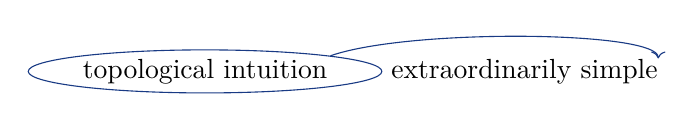
\begin{tikzpicture}[baseline=(a.base)]\node[anchor=base west,draw=blue,ellipse,inner sep=1pt] (a) {topological intuition};\node[anchor=base west,inner sep=0pt,xshift=3pt] (b) at (a.base east) {extraordinarily simple};\draw[blue,->] (a.north east) .. controls +(1,.35) and +(0,.35) .. (b.north east);\end{tikzpicture}}{extraordinarily simple topological intuition}{authorial transposition}{ps_134-2_071-v0007}\hand{,} which I will
make explicit, supposing, to fix the ideas\hand{,} that the base field is $\mathbb{C}$ and so
one may work with locally compact spaces in the usual sense. The topological
idea behind the hypothesis of equi-singularity is that there exists a
\emph{tubular neighbourhood} $T$ of $X_0$ in $X$ retracting onto $X_0$ and such
that the pair $(X_0 , T)$ over $X_0$ should be a locally trivial bundle, i.e.
that $T\backslash X_0$ is locally trivial over $X_0$ . In fact if $\partial T$ is the ``boundary''
of $T$ , which also should be a locally trivial bundle on $X_0$ , then $T$ over
$X$ is the conic bundle (= bundle where fibres are cones) $(\simeq (\partial T \times I) \coprod_{\partial T} X_{\hand{0}}$
\margin{\hand{$\longmapsto$}} where $I = [0, 1]$ , $\partial T \to \partial T \times I$ is defined by $x \var{\over{\to}{\mapsto}}{\hand{\mapsto}}{writing over}{ps_134-2_071-v0008} (x, 1)$ , and
$\partial T \to X_0$ is the projection) then $\overset{\circ}{T} = T\backslash X_0 \simeq \partial T \times [0, 1\hand{[}$ is $X_0$-homotopic
to $\partial T$ . If $X_0$ and $X_{\hand{1}}$ are non singular, then so also will be $\overset{\circ}{T}$ and $\partial T$ ,
which are then topologically smooth fibrations on $X_0$ . Moreover, putting
$\widetilde{X}_1 = X_{\hand{1}}\backslash\overset{\circ}{T}$ , the inclusion $\widetilde{X}_1 \to X_{\hand{1}}$ is a homotopy equivalence, and $X$ can
be recovered, up to homeomorphism, from the diagram of spaces
\diagram{
\begin{tikzcd}
(\overset{\circ}{T} = T\backslash X_0 \cong)\,\partial T \arrow[r, "j", "\text{inclusion}"', color=blue] \arrow[d, "\text{fibration}"', "p", color=blue] \& \widetilde{X}_{\hand{1}}(\cong X_{\hand{1}}) \\
X_0 \&
\end{tikzcd}
}
as an amalgamated sum. In terms of this diagram of spaces, the above functor
$\phi$ interprets immediately as
\[ \phi(F_{\hand{1}}) \simeq p_* j^*(\widetilde{F}_{\hand{1}}) \]
where $F_{\hand{1}} \to \widetilde{F}_{\hand{1}}$ is the restriction from $X_{\hand{1}}$ to $\widetilde{X}_{\hand{1}}$ (which is an equivalence
of categories for the envisaged (locally constant) sheaves). Giving
$F = (F_0 , F_{\hand{1}} , u : F_0 \to \phi F_{\hand{1}})$ can then also be made explicit as giving

\margin{\hand{71}}

%% END SOURCE ps_134-2_071
\ifnum\EditionMode=1
\psapparatusstart
\psentry{ps_134-2_071-v0001}{1}{deletion}{\deleted{for}}{}{The author cancels this material by hand; it leaves the corrected running text.}
\psentry{ps_134-2_071-v0002}{2}{deletion}{\deleted{the fact}}{}{The author cancels this material by hand; it leaves the corrected running text.}
\psentry{ps_134-2_071-v0003}{3}{deletion}{\deleted{satisfying}}{}{The author cancels this material by hand; it leaves the corrected running text.}
\psentry{ps_134-2_071-v0004}{4}{insertion}{\inserted{interesting}}{\hand{interesting}}{The handwritten insertion is incorporated at its indicated position; insertion brackets leave the running text.}
\psentry{ps_134-2_071-v0005}{5}{deletion}{\deleted{sheaf)}}{}{The author cancels this material by hand; it leaves the corrected running text.}
\psentry{ps_134-2_071-v0006}{6}{insertion}{\inserted{scheme}}{\hand{scheme}}{The handwritten insertion is incorporated at its indicated position; insertion brackets leave the running text.}
\psentry{ps_134-2_071-v0007}{7}{authorial transposition}{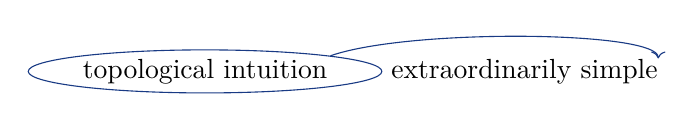
\begin{tikzpicture}[baseline=(a.base)]\node[anchor=base west,draw=blue,ellipse,inner sep=1pt] (a) {topological intuition};\node[anchor=base west,inner sep=0pt,xshift=3pt] (b) at (a.base east) {extraordinarily simple};\draw[blue,->] (a.north east) .. controls +(1,.35) and +(0,.35) .. (b.north east);\end{tikzpicture}}{extraordinarily simple topological intuition}{The pen oval and long arrow move the typed phrase topological intuition after extraordinarily simple; the diplomatic form preserves the earlier order and the visible graphic.}
\psentry{ps_134-2_071-v0008}{8}{writing over}{$\over{\to}{\mapsto}$}{$\hand{\mapsto}$}{The superposed handwritten reading replaces the underlying reading.}
\psapparatusend
\fi
\pssource{ps_134-2_072}{134-2/72}{https://grothendieck.umontpellier.fr/web/viewer.html?file=../134-2.pdf\#page=73}
\psnumber{ps_134-2_072-v0001}{1}
\psnumber{ps_134-2_072-v0002}{2}
\psnumber{ps_134-2_072-v0003}{3}
\psnumber{ps_134-2_072-v0004}{4}
\psnumber{ps_134-2_072-v0005}{5}
\psnumber{ps_134-2_072-v0006}{6}
\psnumber{ps_134-2_072-v0007}{7}
\psnumber{ps_134-2_072-v0008}{8}
\psnumber{ps_134-2_072-v0009}{9}
\psnumber{ps_134-2_072-v0010}{10}
\psnumber{ps_134-2_072-v0011}{11}
\psnumber{ps_134-2_072-v0012}{12}
\psnumber{ps_134-2_072-v0013}{13}
%% BEGIN SOURCE ps_134-2_072
% Pursuing Stacks (cotes 134-2 to 134-8): archive cote 134-2, site page 72 (PDF page 73).
% appendix (letters to Breen). Draft compared: ps1.tex:1577-1605.
% AI-transcribed by Claude Opus 5.5 (claude-opus-5-5, adaptive thinking, effort high), Message Batches API, batch ps1 (msgbatch_01Rv5hCaNTtUt4JHx1yqoHPL), 2026-11-12; reviewed against both supplied scan halves; see CHECK_DECISIONS.tsv.
\scanpage{134-2/72}
\mspage{- \hand{5}7 -}
\[ F_0 \ , \ \widetilde{F}_{\hand{1}} \ , \ \widetilde{u} : p^*(F_0) \to j^*(\widetilde{F}_1) \]
where $F_0(\widetilde{F}_1)$ are locally constant sheaves on $X_0$ (respectively $X_{\hand{1}}$).
It is necessary to recall that \var{\deleted{up to}}{}{deletion}{ps_134-2_072-v0001} here $p$ is a real fibration, and
$j$ is an inclusion (in practice, \var{\deleted{``}}{}{deletion}{ps_134-2_072-v0002}for the case $X_0$ , $X_{\hand{1}}$ smooth\hand{,}\var{\deleted{''}}{}{deletion}{ps_134-2_072-v0003} the
inclusion of the boundary in a manifold with boundary).

If you prefer, one can also take the diagram which is less pretty (but
a little more canonical)
\diagram{\[\begin{tikzcd}
  \overset{\circ}{T} \ar[r,"j'",color=blue]\ar[d,swap,"p'",color=blue] \& X_{\hand{1}} \\
  X_0 \&
\end{tikzcd}\]}
coming essentially to the same thing, as it is formed from spaces homotopic
to the preceding one. One can even replace $X_0$ by $T$ ($X_0$ being a
deformation retract of it) and write
\diagram{\[\begin{tikzcd}
  \overset{\circ}{T} \ar[r,color=blue]\ar[d,swap,"p''",color=blue] \& X_1 \\
  T \&
\end{tikzcd}\]}
where ``literally'' $p''$ is now an inclusion, but ``morally'', it is a \textit{fibration}
with \var{\deleted{a}}{}{deletion}{ps_134-2_072-v0004} very pretty fibres [notably \var{\inserted{compact}}{\hand{compact}}{insertion}{ps_134-2_072-v0005} o\var{\over{\unsure{r|f}}{f}}{\hand{f}}{writing over}{ps_134-2_072-v0006} finite dimension, and \var{\inserted{moreover}}{\hand{moreover}}{insertion}{ps_134-2_072-v0007} \var{\deleted{in fact perhaps}}{}{deletion}{ps_134-2_072-v0008}
non-singular varieties - this is \var{\deleted{\unsure{then}}}{}{deletion}{ps_134-2_072-v0009} much better than that which is given
by the yoga of Cartan-Serre ``every continuous mapping is equivalent to a
fibration''...] . This last diagram \var{\deleted{is}}{}{deletion}{ps_134-2_072-v0010} \var{\inserted{however has the advantage of being}}{\hand{however has the advantage of being}}{insertion}{ps_134-2_072-v0011} amenable to a purely algebraic, direct
construction, in the context of schemes, once one has developed the
construction of étale tubular neighbourhood\hand{s}\hand{\textsuperscript{(28)}}.
\margin{\hand{\tikz[baseline=(x.base)]{\node[draw,ellipse,inner sep=2pt] (x) {espacer};\draw[->] (1,.1)--(.7,.1)--(.7,1.1);\draw[->] (1,-.1) .. controls (.25,-.1) and (.8,-.7) .. (.7,-1.1);\draw (-.15,-.05)--(1.7,-.05);}}}
\margin{\hand{\tikz[baseline=(x.base)]{\node (x) {(App \unsure{17})};\draw (.5,.3)--(.5,.5);\draw (.5,.3) .. controls (-1,.6) and (-1,-.65) .. (.5,-.3)--(.5,-.5);\draw (1.65,.4)--(.95,.4) .. controls (.7,.4) and (.7,-.2) .. (.95,-.2)--(1.65,-.2);}}} The point I wish to come to, is that the consideration of sheaves
(or complexes thereof, or n-stacks ...) which are P-constructible on an $X$ ,
where $P$ is a given ``equi-singular'' stratification, \var{\deleted{comes}}{}{deletion}{ps_134-2_072-v0012} \var{\inserted{reduces}}{\hand{reduces}}{insertion}{ps_134-2_072-v0013} in our particular
cases to the knowledge of a diagram of ordinary \textit{homotopy types} (or pro-types,
if one comes back to the étale topology)

\margin{\hand{72}}

%% END SOURCE ps_134-2_072
\ifnum\EditionMode=1
\psapparatusstart
\psentry{ps_134-2_072-v0001}{1}{deletion}{\deleted{up to}}{}{The author cancels this material by hand; it leaves the corrected running text.}
\psentry{ps_134-2_072-v0002}{2}{deletion}{\deleted{``}}{}{The author cancels this material by hand; it leaves the corrected running text.}
\psentry{ps_134-2_072-v0003}{3}{deletion}{\deleted{''}}{}{The author cancels this material by hand; it leaves the corrected running text.}
\psentry{ps_134-2_072-v0004}{4}{deletion}{\deleted{a}}{}{The author cancels this material by hand; it leaves the corrected running text.}
\psentry{ps_134-2_072-v0005}{5}{insertion}{\inserted{compact}}{\hand{compact}}{The handwritten insertion is incorporated at its indicated position; insertion brackets leave the running text.}
\psentry{ps_134-2_072-v0006}{6}{writing over}{\over{\unsure{r|f}}{f}}{\hand{f}}{The superposed handwritten reading replaces the underlying reading.}
\psentry{ps_134-2_072-v0007}{7}{insertion}{\inserted{moreover}}{\hand{moreover}}{The handwritten insertion is incorporated at its indicated position; insertion brackets leave the running text.}
\psentry{ps_134-2_072-v0008}{8}{deletion}{\deleted{in fact perhaps}}{}{The author cancels this material by hand; it leaves the corrected running text.}
\psentry{ps_134-2_072-v0009}{9}{deletion}{\deleted{\unsure{then}}}{}{The author cancels this material by hand; it leaves the corrected running text.}
\psentry{ps_134-2_072-v0010}{10}{deletion}{\deleted{is}}{}{The author cancels this material by hand; it leaves the corrected running text.}
\psentry{ps_134-2_072-v0011}{11}{insertion}{\inserted{however has the advantage of being}}{\hand{however has the advantage of being}}{The handwritten insertion is incorporated at its indicated position; insertion brackets leave the running text.}
\psentry{ps_134-2_072-v0012}{12}{deletion}{\deleted{comes}}{}{The author cancels this material by hand; it leaves the corrected running text.}
\psentry{ps_134-2_072-v0013}{13}{insertion}{\inserted{reduces}}{\hand{reduces}}{The handwritten insertion is incorporated at its indicated position; insertion brackets leave the running text.}
\psapparatusend
\fi
\pssource{ps_134-2_073}{134-2/73}{https://grothendieck.umontpellier.fr/web/viewer.html?file=../134-2.pdf\#page=74}
\psnumber{ps_134-2_073-v0001}{1}
\psnumber{ps_134-2_073-v0002}{2}
\psnumber{ps_134-2_073-v0003}{3}
\psnumber{ps_134-2_073-v0004}{4}
\psnumber{ps_134-2_073-v0005}{5}
\psnumber{ps_134-2_073-v0006}{6}
\psnumber{ps_134-2_073-v0007}{7}
\psnumber{ps_134-2_073-v0008}{8}
\psnumber{ps_134-2_073-v0009}{9}
\psnumber{ps_134-2_073-v0010}{10}
\psnumber{ps_134-2_073-v0011}{11}
\psnumber{ps_134-2_073-v0012}{12}
\psnumber{ps_134-2_073-v0013}{13}
\psnumber{ps_134-2_073-v0014}{14}
%% BEGIN SOURCE ps_134-2_073
% Pursuing Stacks (cotes 134-2 to 134-8): archive cote 134-2, site page 73 (PDF page 74).
% appendix (letters to Breen). Draft compared: ps1.tex:1600-1612.
% AI-transcribed by Claude Opus 5.5 (claude-opus-5-5, adaptive thinking, effort high), Message Batches API, batch ps1 (msgbatch_01Rv5hCaNTtUt4JHx1yqoHPL), 2026-11-12; reviewed against both supplied scan halves; see CHECK_DECISIONS.tsv.
\scanpage{134-2/73}
\mspage{- \hand{5}8 -}

\diagram{\begin{tikzcd}
\Delta \arrow[r, "j",color=blue] \arrow[d, "p"',color=blue] \& X_{\hand{1}} \\
X_0 \&
\end{tikzcd}}

by taking local coefficients systems (or locally constant n-stacks) on
the vertices $X_0$ , $X_1$ , which are related to each other by a hom\var{\deleted{e}}{}{deletion}{ps_134-2_073-v0001}omorphism
of compatibility of the type $p^*(F_0)\hand{\to} j^*(F_{\hand{1}})$ . It should be an amusing
excercise (which I have not yet done) to verify and to make explicit how
the \var{\deleted{usual}}{}{deletion}{ps_134-2_073-v0002} \var{\inserted{``six}}{\hand{``six}}{insertion}{ps_134-2_073-v0003} operations'' on sheaves (\var{\inserted{either}}{\hand{either}}{insertion}{ps_134-2_073-v0004} on $X$ , or on a \var{\inserted{subspace which is a}}{\hand{subspace which is a}}{insertion}{ps_134-2_073-v0005} union of strata of $X$ )
can be expressed in this dictionary, in the case, let us say, of non-singular
strata (otherwise, there will be a difficulty with the duali\var{\over{z}{s}}{\hand{s}}{writing over}{ps_134-2_073-v0006}ing complexes,
which one would prefer to have as objects in our category\hand{)}\hand{,} and \var{\deleted{with re-}}{}{deletion}{ps_134-2_073-v0007} \var{\inserted{to reestablish}}{\hand{to reestablish}}{insertion}{ps_134-2_073-v0008}
\var{\deleted{verifying}}{}{deletion}{ps_134-2_073-v0009} the known formulae involving these operations\var{\deleted{)}}{}{deletion}{ps_134-2_073-v0010}. But it appears
probable that, to carry out this transcription well, it would be necessary,
rather than considering a diagram of type

\diagram{\begin{tikzcd}
\bullet \arrow[r,color=blue] \arrow[d,color=blue] \& \bullet \\
\bullet \&
\end{tikzcd}}

in the homotopical category formed from the category of semi-simplicial sets,
to consider the category of diagrams of semi-simplicial sets, and to pass from
these to the homotopical category of fractions\hand{(\unsure{29})}.

I have recently more or less made explicit, while thinking on the
foundations of ``tame topology'', (i.e. where one \var{\deleted{immediately}}{}{deletion}{ps_134-2_073-v0011} eliminates \var{\inserted{from start}}{\hand{from start}}{insertion}{ps_134-2_073-v0012} all
wild phenomena) how an equisingular stratification, say with non singular
strata, of a compact ``tame space'', gives rise canonically to a diagram of spaces
which are manifolds with boundary,  the arrows of the diagram being essentially
locally trivial fibrations of manifolds with boundary on the others (with
fibres \var{\inserted{which are compact}}{\hand{which are compact}}{insertion}{ps_134-2_073-v0013} manifolds with boundary), \textit{and} the inclusions of the boundar\var{\over{y}{ies}}{\hand{ies}}{writing over}{ps_134-2_073-v0014} in these
manifolds with boundary [in fact, one finds slightly more general inclusions,
certain boundaries which appear being endowed with an ``elementary'' cellular

\margin{\hand{73}}

%% END SOURCE ps_134-2_073
\ifnum\EditionMode=1
\psapparatusstart
\psentry{ps_134-2_073-v0001}{1}{deletion}{\deleted{e}}{}{The author cancels this material by hand; it leaves the corrected running text.}
\psentry{ps_134-2_073-v0002}{2}{deletion}{\deleted{usual}}{}{The author cancels this material by hand; it leaves the corrected running text.}
\psentry{ps_134-2_073-v0003}{3}{insertion}{\inserted{``six}}{\hand{``six}}{The handwritten insertion is incorporated at its indicated position; insertion brackets leave the running text.}
\psentry{ps_134-2_073-v0004}{4}{insertion}{\inserted{either}}{\hand{either}}{The handwritten insertion is incorporated at its indicated position; insertion brackets leave the running text.}
\psentry{ps_134-2_073-v0005}{5}{insertion}{\inserted{subspace which is a}}{\hand{subspace which is a}}{The handwritten insertion is incorporated at its indicated position; insertion brackets leave the running text.}
\psentry{ps_134-2_073-v0006}{6}{writing over}{\over{z}{s}}{\hand{s}}{The superposed handwritten reading replaces the underlying reading.}
\psentry{ps_134-2_073-v0007}{7}{deletion}{\deleted{with re-}}{}{The author cancels this material by hand; it leaves the corrected running text.}
\psentry{ps_134-2_073-v0008}{8}{insertion}{\inserted{to reestablish}}{\hand{to reestablish}}{The handwritten insertion is incorporated at its indicated position; insertion brackets leave the running text.}
\psentry{ps_134-2_073-v0009}{9}{deletion}{\deleted{verifying}}{}{The author cancels this material by hand; it leaves the corrected running text.}
\psentry{ps_134-2_073-v0010}{10}{deletion}{\deleted{)}}{}{The author cancels this material by hand; it leaves the corrected running text.}
\psentry{ps_134-2_073-v0011}{11}{deletion}{\deleted{immediately}}{}{The author cancels this material by hand; it leaves the corrected running text.}
\psentry{ps_134-2_073-v0012}{12}{insertion}{\inserted{from start}}{\hand{from start}}{The handwritten insertion is incorporated at its indicated position; insertion brackets leave the running text.}
\psentry{ps_134-2_073-v0013}{13}{insertion}{\inserted{which are compact}}{\hand{which are compact}}{The handwritten insertion is incorporated at its indicated position; insertion brackets leave the running text.}
\psentry{ps_134-2_073-v0014}{14}{writing over}{\over{y}{ies}}{\hand{ies}}{The superposed handwritten reading replaces the underlying reading.}
\psapparatusend
\fi
\pssource{ps_134-2_074}{134-2/74}{https://grothendieck.umontpellier.fr/web/viewer.html?file=../134-2.pdf\#page=75}
\psnumber{ps_134-2_074-v0001}{1}
\psnumber{ps_134-2_074-v0002}{2}
\psnumber{ps_134-2_074-v0003}{3}
\psnumber{ps_134-2_074-v0004}{4}
\psnumber{ps_134-2_074-v0005}{5}
\psnumber{ps_134-2_074-v0006}{6}
\psnumber{ps_134-2_074-v0007}{7}
\psnumber{ps_134-2_074-v0008}{8}
\psnumber{ps_134-2_074-v0009}{9}
\psnumber{ps_134-2_074-v0010}{10}
\psnumber{ps_134-2_074-v0011}{11}
\psnumber{ps_134-2_074-v0012}{12}
\psnumber{ps_134-2_074-v0013}{13}
\psnumber{ps_134-2_074-v0014}{14}
%% BEGIN SOURCE ps_134-2_074
% Pursuing Stacks (cotes 134-2 to 134-8): archive cote 134-2, site page 74 (PDF page 75).
% appendix (letters to Breen). Draft compared: ps1.tex:1597-1614.
% AI-transcribed by Claude Opus 5.5 (claude-opus-5-5, adaptive thinking, effort high), Message Batches API, batch ps1 (msgbatch_01Rv5hCaNTtUt4JHx1yqoHPL), 2026-11-12; reviewed against both supplied scan halves; see CHECK_DECISIONS.tsv.
\scanpage{134-2/74}
\mspage{- \hand{5}9 -}

decomposition, i.e. the closed strata are again manifolds with boundary which
are glued together along common parts of the boundary; and it is also
necessary to consider the inclusions of these pieces one in\var{\inserted{to}}{\hand{to}}{insertion}{ps_134-2_074-v0001} another ...],
and can be reconstituted from this diagram by gluing\hand{(30)}.In other words, one
has a canonical devissage description of tame compact spaces $X$ , eventually
endowed with equi-singular stratifications with non-singular strata, in terms
of finite diagrams of a precise nature made out of manifolds with boundary.
When \var{\deleted{in a situation of}}{}{deletion}{ps_134-2_074-v0002}\var{\inserted{we are interested in}}{\hand{we are interested in}}{insertion}{ps_134-2_074-v0003} sheaves (or complexes of sheaves\hand{,} or n-stacks) which
are P-constructible on $X$ , where $P$ is such a fixed stratification, \var{\deleted{known}}{}{deletion}{ps_134-2_074-v0004}\var{\inserted{these}}{\hand{these}}{insertion}{ps_134-2_074-v0005}
\var{\deleted{explicitly}}{}{deletion}{ps_134-2_074-v0006}\var{\inserted{may be described}}{\hand{may be described}}{insertion}{ps_134-2_074-v0007} in terms of the envisaged diagram\hand{,}of which only the ``homotopy
type'' is to be retained. One \var{\deleted{observes}}{}{deletion}{ps_134-2_074-v0008}\var{\inserted{foresees}}{\hand{foresees}}{insertion}{ps_134-2_074-v0009} that the six operations on these sheaves
can be translated in an ad hoc manner to this homotopical context. Finally\hand{,}
if instead of having only one compact tame space $X$ , one has, let us say,
a tame morphism $f : X \to Y$ of such objects, then \var{\deleted{by devissage of}}{}{deletion}{ps_134-2_074-v0010}\var{\inserted{by choosing}}{\hand{by choosing}}{insertion}{ps_134-2_074-v0011} equi-%
singular stratifications on $X$ and $Y$ adapted to $f$ (the strata of $X$
being in particular locally trivial fibrations on those of $Y$ ...), one
should find a ``morphism'' from the diagram of manifolds with boundary
expressing $X$ into that expressing $Y$ (with \var{\deleted{some natural}}{}{deletion}{ps_134-2_074-v0012}\var{\inserted{mutal}}{\hand{mutal}}{insertion}{ps_134-2_074-v0013} morphisms which
essentially reduce to fibrations of \var{\inserted{compact}}{\hand{compact}}{insertion}{ps_134-2_074-v0014} manifolds with boundaries on other such
objects) in such a way that the four operations $Rf_*$, $Rf_!$, $Lg^*$, $g^!$ between
$P_X$- and $P_Y$- constructible sheaves on $X$ and $Y$ (or on locally closed
sub spaces $X'$ , $Y'$ which are union of strata, such that $f$ induces
$g : X' \to Y'$) can be expressed in terms of standard operations between the
mere homotopy type\hand{s}. Finally, all these constructions, still partially
hypothetical (there is work on the foundations to be done!) should be able
to be paraphrased in the framework of excellent schemes, by making use of
the machinery of étale tubular neighbourhoods. In one or other case, the
``fine homotopy type'' of a tame space, respectively of an excellent scheme,
is defined by passage to the limit from ``P-homotopy type'' associated to finer
and finer equi-singular stratifications $P$ (with non-singular strata).

\margin{\hand{74}}

%% END SOURCE ps_134-2_074
\ifnum\EditionMode=1
\psapparatusstart
\psentry{ps_134-2_074-v0001}{1}{insertion}{\inserted{to}}{\hand{to}}{The handwritten insertion is incorporated at its indicated position; insertion brackets leave the running text.}
\psentry{ps_134-2_074-v0002}{2}{deletion}{\deleted{in a situation of}}{}{The author cancels this material by hand; it leaves the corrected running text.}
\psentry{ps_134-2_074-v0003}{3}{insertion}{\inserted{we are interested in}}{\hand{we are interested in}}{The handwritten insertion is incorporated at its indicated position; insertion brackets leave the running text.}
\psentry{ps_134-2_074-v0004}{4}{deletion}{\deleted{known}}{}{The author cancels this material by hand; it leaves the corrected running text.}
\psentry{ps_134-2_074-v0005}{5}{insertion}{\inserted{these}}{\hand{these}}{The handwritten insertion is incorporated at its indicated position; insertion brackets leave the running text.}
\psentry{ps_134-2_074-v0006}{6}{deletion}{\deleted{explicitly}}{}{The author cancels this material by hand; it leaves the corrected running text.}
\psentry{ps_134-2_074-v0007}{7}{insertion}{\inserted{may be described}}{\hand{may be described}}{The handwritten insertion is incorporated at its indicated position; insertion brackets leave the running text.}
\psentry{ps_134-2_074-v0008}{8}{deletion}{\deleted{observes}}{}{The author cancels this material by hand; it leaves the corrected running text.}
\psentry{ps_134-2_074-v0009}{9}{insertion}{\inserted{foresees}}{\hand{foresees}}{The handwritten insertion is incorporated at its indicated position; insertion brackets leave the running text.}
\psentry{ps_134-2_074-v0010}{10}{deletion}{\deleted{by devissage of}}{}{The author cancels this material by hand; it leaves the corrected running text.}
\psentry{ps_134-2_074-v0011}{11}{insertion}{\inserted{by choosing}}{\hand{by choosing}}{The handwritten insertion is incorporated at its indicated position; insertion brackets leave the running text.}
\psentry{ps_134-2_074-v0012}{12}{deletion}{\deleted{some natural}}{}{The author cancels this material by hand; it leaves the corrected running text.}
\psentry{ps_134-2_074-v0013}{13}{insertion}{\inserted{mutal}}{\hand{mutal}}{The handwritten insertion is incorporated at its indicated position; insertion brackets leave the running text.}
\psentry{ps_134-2_074-v0014}{14}{insertion}{\inserted{compact}}{\hand{compact}}{The handwritten insertion is incorporated at its indicated position; insertion brackets leave the running text.}
\psapparatusend
\fi

\end{document}
